%%%%%%%%%%%%%%%%%%%%%%%%%%%%%%%%%%%%%%%%%%%%%%%%%%%%
%%%     Dissertation Master File                 %%%
%%%    based on Language Science Press template  %%%
%%%%%%%%%%%%%%%%%%%%%%%%%%%%%%%%%%%%%%%%%%%%%%%%%%%%

\documentclass[output=book,
% citecolor=black
%  ,colorlinks
%  ,draft
% ,draftmode,
%  booklanguage=german,
		  ]{langscibook}
		  
%%%%%%%%%%%%%%%%%%%%%%%%%%%%%%%%%%%%%%%%%%%%%%%%%%%%
%%%          additional packages                 %%%
%%%%%%%%%%%%%%%%%%%%%%%%%%%%%%%%%%%%%%%%%%%%%%%%%%%%

\author{Janne Marike Lorenzen}
\title{Individual variability in the encoding and decoding of prosodic prominence relations}
\subtitle{}
\BackTitle{Individual variability in the encoding and decoding of prosodic prominence relations}


\renewcommand{\lsID}{611}
\renewcommand{\lsSeries}{silp}
\renewcommand{\lsSeriesNumber}{18}
\ISBNdigital{978-3-96110-590-8}
\ISBNhardcover{978-3-98554-207-9}
\BookDOI{10.5281/zenodo.21133333}

\BackBody{This book investigates inter-individual variability in the encoding and decoding of prosodic prominence relations. Formally, prosodic prominence relations are redundantly expressed by several acoustic parameters, such as changes in fundamental frequency, duration, and intensity. Functionally, prominence relations encode meaning, e.g., the information status of a word or referent. Both the formal and the functional side of prominence facilitate inter-individual variability. On the one hand, redundancy inherent in prominence marking enables individuals to use different parameters in their production and perception. On the other hand, differences in communicative skills may influence which meaning aspects language users pay attention to and how strongly they encode them.

In this book, inter-individual variability is analyzed in two production studies and one perception study. Production data is elicited in listener-directed reading tasks and analyzed using prosodic annotation and acoustic analyses. Perception is probed via a prominence rating task. Individual differences are explored via careful descriptive inspection of the data and statistically via cluster analyses. Results indicate that speakers differ in how strongly they encode prominence relations, which parameters they use to do so, and which meaning aspects they predominantly mark - which in turn is partially modulated by their communicative skills. Listeners also vary in their sensitivity to prominence cues.

These findings highlight the importance of looking at the individual speaker or listener in prosodic research and allow for a new perspective on established concepts in prosodic theory, such as
the dichotomy of tune and metrical structure, relationality and redundancy in
prominence encoding and decoding, and the probabilistic nature of form-meaning mapping.
}

\renewcommand{\lsImpressumExtra}{The work presented in this book is based on the author's doctoral dissertation, which was accepted by the Faculty of Arts and Humanities at the University of Cologne in 2024.}

\typesetter{Janne Marike Lorenzen}
\proofreader{Matthew Korte}


\usepackage{langsci-optional}
\usepackage{langsci-gb4e}
\usepackage{langsci-lgr}
\usepackage{langsci-branding}
\usepackage{listings}
\lstset{basicstyle=\ttfamily,tabsize=2,breaklines=true}

\usepackage{appendix}

%Here is the hypersetup to control the colors of table of contents etc.
% \hypersetup{
%     hidelinks=true,
%     colorlinks=true,
%     linkcolor=black,
%     filecolor=black,
%     citecolor=black,
%     urlcolor=blue
%     }

%Defining with which chapter number to start. This is useful when you want to send individual chapters
%\setcounter{chapter}{0}
%setting the Table of Contents (TOC) depth. Zero {0} shows only the name of the chapter
%\setcounter{tocdepth}{4}

% \usepackage[backend=biber, style=ieee]{biblatex} 
% \DeclareSourcemap{
%   \maps[datatype=bibtex]{
%     \map{
%       \step[fieldset=urldate, null]
%     }
%   }
% }

% \usepackage{graphicx}
\graphicspath{ {./figures/} }

\usepackage{subfig}

\usepackage{enumitem}
% \setlist{itemsep=0pt}

\usepackage{multirow}

\usepackage{soul}

% \usepackage{tabularx}
\usepackage[table,xcdraw]{xcolor}

%\usepackage{pdfpages}

%% hyphenation points for line breaks
%% Normally, automatic hyphenation in LaTeX is very good
%% If a word is mis-hyphenated, add it to this file
%%
%% add information to TeX file before \begin{document with:
%% \include{localhyphenation
\hyphenation{
par-a-digm
off-glide
new/con-tras-tive
pro-so-dy
pro-sodic
lear-ning/sto-rage
con-tras-tive
new-ness
com-mu-ni-ca-tive-ly
know-ledge
Plätz-chen
letz-te
Ke-ra-mik-ar-ti-kel
Ge-schäft
Werk-zeug-samm-lung
an-zu-se-hen
ein-kau-fen
he-raus-ge-nom-men
he-raus-ge-sucht
}

\addbibresource{bibliography.bib}

%%%%%%%%%%%%%%%%%%%%%%%%%%%%%%%%%%%%%%%%%%%%%%%%%%%%
%%%             Frontmatter                      %%%
%%%%%%%%%%%%%%%%%%%%%%%%%%%%%%%%%%%%%%%%%%%%%%%%%%%%
\begin{document}
% \newcommand*{\orcid}{}

\newcommand{\pkg}[1]{{\normalfont\fontshape{it}\selectfont #1}}
 

\maketitle
\frontmatter
\currentpdfbookmark{Contents}{name} % adds a PDF bookmark
{\sloppy\tableofcontents}
%\listoffigures
%\listoftables
%  \addchap{\lsPrefaceTitle}
 
 
 
  \addchap{\lsAcknowledgementTitle} 

This book is based on my doctoral dissertation, which was accepted by the Faculty of Arts and Humanities at the University of Cologne in 2024. I am grateful to the SFB 1252 ``Prominence in Language" for supporting and funding my doctoral studies. 

Most importantly, I want to thank my committee members, Stefan Baumann, Martine Grice, and Christiane Ulbrich. Stefan, I truly could not have asked for a better supervisor. Working with you has been easy, comfortable, and fun from the beginning. I appreciate your ongoing support throughout this journey and your genuine enthusiasm for prosodic research, which has always been a source of inspiration and motivation. Martine, thank you for becoming my second supervisor. You always have an insightful comment to share and as head of the phonetics institute, you created a supportive, open, and pleasant atmosphere, providing the ideal environment to pursuing a doctorate. Christiane, thank you for joining my committee last minute with such enthusiasm and kindness. It has been a pleasure getting to know you and having you on board for the final stretch of this endeavor.

Several other people have also shaped my dissertation in various ways. Simon Roessig, I was so lucky to collaborate with you and Stefan in the beginning of my doctoral studies. I learned so much from you during these first months, which has really shaped my path. Aviad Albert, thank you for inventing the brilliant ProPer tool and for always taking the time to answer my questions. Heiko Seeliger, thank you for many great insights, always delivered in an enthusiastic yet calm manner. Thank you also to Jason Bishop and Chigusa Kurumada for taking an interest in my research, inspiring me through your research, and cheering me on.

\largerpage
I also want to thank my fellow doctoral students for creating a great sense of community. Special thanks to Maria, I loved sharing an office, all my (sometimes irrational) fears and insecurities but also successes with you. Talking to you has helped me so many times, whether it was statistics advice or your calm reassurance that everything will be fine. Barbara, thank you for making me move (literally) during the last year of our doctoral studies together. It was a pleasure crossing the (metaphorical) finish line together (but I will not run a marathon with you). Mandy, thank you for always bringing good vibes and sometimes brownies.

At the phonetics lab, multiple people have contributed to creating a welcoming and friendly atmosphere, including Elina, Lena, Eduardo, Alicia, Malin, Francesco, Simona, Vatho, Tabea, Simon W., Florence, Katinka, Solveigh, Nadia, Doris, and of course Theo.

At the House of Prominence, I am especially grateful to Constantijn, Mark, Maria B., Timo, Sophia, Katharina, Magdalena, Fafa, Christine, Juman, Job, and Clare for all the joint lunches, coffee and ice cream breaks, and of course Beer Thursdays.

Julia and Sölve, thank you for proofreading all the chapters I sent you in record time. This was just one way of showing your support for me, I am also grateful for everything else.

Thank you to my family for your love and confidence in me, even though academia in general and the field of linguistics in particular probably still remain a mystery to you. Knowing that I chose a path that makes me happy was enough for you to support me unconditionally and for that I am immensely grateful.

Kerem, thank you for being there for me throughout this whole adventure. Whether it is helping me solve a programming problem or building up my confidence, your support means so much to me.

  \addchap{\lsAbbreviationsTitle}
% \addchap{Abbreviations and symbols}

\begin{tabularx}{.45\textwidth}{lQ}
AM & Autosegmental-metrical\\
AQ & Autism-Spectrum Quotient\\
CoG & Center of Gravity\\
CoM & Center of Mass\\
CrI & Credible Interval\\
DIMA & Deutsche Intonation --- Modellierung und Annotation `German Intonation -- Modeling and annotation'\\
EQ & Empathy Quotient\\
F0 & Fundamental frequency\\
GToBI & German Tones and Break Indices\\
H & High\\
Hz & Hertz\\
ip & Intermediate Phrase\\
\\
\end{tabularx}
\begin{tabularx}{.45\textwidth}{lQ}
IP & Intonation Phrase\\
IPO & Institute for Perception Research\\
L & Low\\
L-given & Lexically given\\
L-new & Lexically new\\
RMITE & Reading the Mind in the Eyes\\
RPT & Rapid Prosody Transcription\\
R-given & Referentially given\\
R-new & Referentially new\\
SSRH & Smooth Signal Redundancy Hypothesis\\
TCoG & Tonal Center of Gravity\\
ToBI & Tones and Break Indices\\
\\
\end{tabularx}



\mainmatter

%%%%%%%%%%%%%%%%%%%%%%%%%%%%%%%%%%%%%%%%%%%%%%%%%%%%
%%%             Chapters                         %%%
%%%%%%%%%%%%%%%%%%%%%%%%%%%%%%%%%%%%%%%%%%%%%%%%%%%%

\chapter{Introduction}

Inter-individual variability is ubiquitous in speech production and perception (see, e.g., \citealt{yuIndividualDifferencesLanguage2019} for a review of studies on individual variability in segmental processing). Prosody is no exception to this phenomenon. In fact, prosodic prominence, e.g., the employment of accent, is a system that lends itself especially readily to substantial variability. In the aptly titled journal paper ``Accent is predictable (if you're a mind reader)", \citet{bolingerAccentPredictableIf1972} expresses the idea that accent placement predominantly reflects a speaker's intent in structuring information.
Intent is naturally subjective and thus highly likely to give rise to variable productions across similar conditions. 
 
In West-Germanic languages, prominence encodes aspects of meaning, such as focus or information status \citep{buringSemanticsIntonationInformation2007, feryPitchAccentScaling2008, baumannCoreferenceLexicalGivenness2013, coleProsodyContextReview2015}. The most informative part of an utterance is understood as in \textit{focus}, other parts are in the \textit{background} \citep{buringSemanticsIntonationInformation2007}. Often the constituent in focus at the same time introduces \textit{new} information to the discourse, but this is not necessarily the case, so that information status can be regarded as an independent meaning dimension. Focus and information status can be subsumed under the general notion of information structure \citep{hallidayNotesTransitivityTheme1967}. Structuring information with regard to the preceding discourse is a basic communicative function that allows discourse participants to establish and manage common ground \citep{krifkaBasicNotionsInformation2008}. Parts of an utterance can be presented in focus or in the background, as contrastive or non-contrastive, and as new or given information \citep{buringSemanticsIntonationInformation2007}.

These meaning contrasts are encoded in the prominence \textit{relations} of prosodic constituents, which can be expressed by different (combinations of) prosodic parameters, such as changes in the fundamental frequency (F0), duration, and intensity \citep{fryDurationIntensityPhysical1955, sluijterSpectralBalanceAcoustic1996, kochanskiLoudnessPredictsProminence2005, baumannWhatMakesWord2018, roessigTracingPhoneticSpace2022}.
This potential redundancy allows individuals to rely on different aspects of the signal in prominence production and perception.
Relationality and redundancy can thus be regarded as key notions of prominence that enable and drive inter-individual variability.

In prosodic research, this variability has often been treated as noise and thus largely ignored \citep{arvanitiVariabilityOverlapCue2024}. With the advance of empirical methods, such as mixed-effects regression modeling, variability introduced by speakers or listeners is now usually accounted for in a random effects structure \citep[e.g.,][]{winterStatisticsLinguistsIntroduction2020, winterIndependenceGeneralizabilityLinguistics2021}. At least implicitly, inter-individual variability is thus acknowledged by most empirical studies that adhere to these standards, although generally only with the aim to control for this variability and thus clean up group-level effects.

Interest in individual variability from a theoretical point of view has also recently been on the rise. Promising lines of research address prosodic trade-off effects, cue weighting, and processing difficulties in the light of a lack of invariance of prosodic categories and form-meaning mapping \citep{kurumadaThinkingProbabilisticallyStudy2021, arvanitiVariabilityOverlapCue2024, severijnenYourVOORnaamNot2024}. Beyond these studies, explicit mentions of individual differences are also increasing in recent prosodic research, reflecting an effort towards greater empirical accuracy \citep[e.g.,][]{cangemiListenerSpecificPerceptionSpeakerSpecific2015, ouyangIndividualDifferencesProsodic2015, baumannWhatMakesWord2018, esteve-gibertEmpathyInfluencesHow2020}.

Nevertheless, systematic investigations into individual differences in prosody are still rare and thus the nature of this variability and mechanisms potentially underlying it are not yet well understood. Especially in the domain of prosody-meaning mapping, previous studies have concentrated on focus marking, neglecting other aspects of information structure. This book seeks to contribute to the emerging research concerned with individual variability in prosody production and perception. Specifically, we explore how and to what extent speakers and listeners vary in their encoding and decoding of prosodic prominence relations, both in terms of strength of encoding and types of parameters employed. Information status serves as the main prosodically encoded meaning aspect investigated here, but additionally, we consider syntactic factors that are known to interact with prosodic structure, namely grammatical role and sentence position. 

Furthermore, we take into account individuals' communicative skill as a potential influence on form-meaning mapping. Differences in communicative skill have previously been related to varying sensitivity to prosody \citep{bishopPhonologyPhoneticsSignalextrinsic2020, orricoInfluenceEmpathyAutisticlike2023} and pragmatic processing abilities \citep{nieuwlandIncrementalityPragmaticProcessing2010, zhaoAreScalarImplicatures2015} and are thus considered here as a potential explanation for inter-individual variability in prominence production and perception.

Empirical findings from two production studies and one perception study are presented and discussed in this book. These studies focus on eliciting speech and perception data from German native speakers in different information status conditions and syntactic structures. In the production experiments, participants produce highly scripted speech in reading tasks to allow for maximum control over the manipulations in the target utterances. To introduce some degree of naturalness, tasks are designed to be listener-directed and include an interactive component. In particular, the first production study investigates stories read by 32 speakers, containing target words that are either discourse new or accessible through the context. In the second production study, we analyze recordings of 20 speakers producing stories that contain target words varying in lexical and referential information status, grammatical role, and sentence position. In the perception study, we elicit prominence ratings on target words presented in context from 65 listeners to probe the effects of prosodic and non-prosodic effects on prominence perception. Here, we use recordings from the second production study as stimuli, including a variety of prosodic and syntactic structures as well as words representing different information status categories.

This book is firmly rooted in autosegmental-metrical theory \citep{laddIntonationalPhonology2008} and considers not only continuous but also categorical parameters associated with a prosodic hierarchy. This allows for direct implications for prosodic theory to be drawn. In terms of continuous measures, we rely on the recently proposed ProPer measures \citep{albertModelSonorityBased2023}, which are signal-based and derivable with minimal manual analysis steps. The same prosodic parameters are considered in all data analyses to allow for comparisons across studies.

In all three studies, we take an exploratory approach to the respective research questions. Exploratory data analysis as opposed to confirmatory analysis focuses on finding new patterns in the data rather than testing established hypotheses via rigorous hypothesis tests \citep{roettgerEmergentDataAnalysis2019}. There are two main reasons underlying the choice of an exploratory approach in this book. Firstly, individual differences in prosody-meaning mapping are not particularly well studied, so that formulating hypotheses with regard to the extent and nature of variability that we expect to observe is not a straightforward task. Secondly, some methods of statistical analysis that are used in this book are inherently exploratory, aiming to mine data for new patterns and not allowing for confirmatory hypothesis testing, e.g., random forest analysis and cluster analysis. Nevertheless, we will formulate expectations based on previous literature that will be tested against the data, but acknowledge that our results may well differ from these \citep{rubinExploratoryHypothesisTests2022}. Some aspects of these analyses are naturally more confirmatory than others, since more research is available to base assumptions on, especially with regard to general across-speaker analyses.

To accompany this exploratory approach, we conduct our statistical analyses in the Bayesian framework. While frequentist frameworks typically support a binary decision with regard to significance, the Bayesian framework allows for the quantification of uncertainty regarding the observed effects \citep{vasishthBayesianDataAnalysis2018}. Another practical advantage is that more complex models can be fitted in the Bayesian framework \citep{vasishthBayesianDataAnalysis2018}. Random slopes are often the first parameter to be dropped from frequentist mixed-effects regression models in cases of convergence issues \citep{barrRandomEffectsStructure2013}. However, these random slopes are crucial in the study of inter-individual variability, so that the Bayesian framework is deemed the best fit for the present investigation.

This book is structured as follows: Chapter \ref{ch:background prominence} outlines the concept of prominence underlying the current work and summarizes insights on prosodic structure, acoustic correlates of prominence, information structure, and interactions between prosody and lexical and syntactic factors, concluding with a discussion of the concept of redundancy in prominence marking and its implications for the emergence of individual variability. This chapter crucially motivates the parameters investigated in the production and perception experiments. Chapter \ref{ch:background variability} provides an overview of previous findings related to individual variability in prosody production and perception and discusses some potential causes, such as communicative skill, empathy, sociodemographic factors, and experience. Chapters \ref{ch:Production I} to \ref{ch: Perception} present the production and perception studies. In the first production study in Chapter \ref{ch:Production I}, we investigate individual variability in the prosodic encoding of information status. This is a first exploration of differences and similarities across speakers varying only one aspect of meaning, while at the same time comparing descriptive and more systematic analytic approaches to the data. The second production study presented in Chapter \ref{ch:Production II} expands on these findings by teasing apart the lexical and the referential level of information status and adding syntactic factors, namely grammatical role and sentence position. Communicative skill is also investigated as a potential factor modulating differences in prominence production across speakers. In Chapter \ref{ch: Perception}, we present a perception study that contributes to the understanding of individual variability with a prominence rating task. In particular, we explore how individuals differ with regard to their usage of prosodic and non-prosodic factors in decoding prominence relations. We again consider communicative skill as a potential underlying mechanism. Chapter \ref{ch: general discussion} brings together all findings in a general discussion and draws final conclusions on the main contributions of this book.
\chapter{Forms and functions of prosodic prominence} \label{ch:background prominence}

Prominence is a somewhat elusive concept and defining it is notoriously difficult. Many attempts have been put forward, which are often characterized by considerable vagueness and sometimes even contradictoriness \citep{cangemiIntegratingPhoneticsPhonology2020}. Common approaches draw on perception and define prominence in terms of its function. For example, Büring describes prominence as ``a speaker's intuitive sensation of strength in an utterance he or she hears" \citeyearpar[1]{buringIntonationMeaning2016}. Similarly, other definitions reference its ability to make entities \textit{stand out} from their context \citep{terkenFundamentalFrequencyPerceived1991, terkenPerceptionProsodicProminence2000} or \textit{highlight} important information \citep{cangemiIntegratingPhoneticsPhonology2020}. 
	
Two notions that are viewed as central to the concept of prominence in the present book are \textit{relationality} and \textit{redundancy}. As the definitions recited above emphasize, prominent entities stand out from their context by somehow being stronger. These definitions underline the relational aspect of prominence: What is prominent is determined by direct comparison to surrounding entities. An entity that is prominent in one context can even be less prominent than an entity that is considered non-prominent in a different context \citep{cangemiIntegratingPhoneticsPhonology2020}. From an acoustic point of view, this highlighting can be achieved via multiple different prosodic cues related to intonation, timing, and power of the signal \citep[e.g.,][]{fryDurationIntensityPhysical1955, sluijterSpectralBalanceAcoustic1996, kochanskiLoudnessPredictsProminence2005, baumannWhatMakesWord2018, roessigTracingPhoneticSpace2022}. The marking of prominence is thus redundant in nature: When one cue fails or is missing, other cues are available to compensate \citep{winterSpokenLanguageAchieves2014}. Speakers may exploit this redundancy by choosing from the available cues when producing prominence. 

Highlighting or making something stand out can serve multiple pragmatic functions, e.g., marking focus or information status. \citep[e.g.,][]{buringSemanticsIntonationInformation2007, feryPitchAccentScaling2008, baumannCoreferenceLexicalGivenness2013, coleProsodyContextReview2015}. In addition, prosody interacts with syntactic structure. These relations will be explored in more detail in the following sections.

Two clarifying notes on terminology are in order at this point. First, prominence in this book should be understood to refer to \textit{prosodic} prominence unless otherwise specified. This caveat may have been superfluous at one time, however, recent research has advanced the notion of prominence as an organizing principle of language at several levels, including discourse meaning and morphosyntax \citep{himmelmannProminenceProsodyFirst2015, vonheusingerDiscourseProminenceDefinition2019}. Second, prosodic prominence is understood as a post-lexical phenomenon. The term \textit{stress} will be used to refer to word-level ``prominence". 

The following sections will take a closer look at prominence from a formal and a functional perspective. First, Section \ref{section: prominence form} provides an overview of formal aspects of prosodic prominence, both in terms of structural prosodic prominence in the framework of Autosegmental-Metrical Theory (Section \ref{section: structural prominence}) and acoustic correlates of prominence (Section \ref{section: acoustics}). In Section \ref{section: Information structure}, we turn to functional aspects of prominence, specifically information structure marking. Section \ref{section: lexical and syntactic} reports on lexical and syntactic influences on prominence. Finally, Section \ref{section: redundancy} summarizes the previous sections with a view on redundancy and its implications for individual variability in prominence production and perception.

\section{Prosodic prominence: Formal aspects} \label{section: prominence form}

\subsection{Prosodic structure} \label{section: structural prominence}

The present book follows the influential Autosegmental-Metrical (AM) theory of prosody \citep{laddIntonationalPhonology2008}, which builds on the insights of \citet{libermanIntonationalSystemEnglish1975}, \citet{bruceSwedishWordAccents1977}, and \citet{pierrehumbertPhonologyPhoneticsEnglish1980}. Within this framework, prosodic constituents are viewed as hierarchically organized \citep{selkirkPhonologySyntaxRelation1984, hayesProsodicHierarchyMeter1989}. Relevant prosodic layers include the intonation phrase, the intermediate phrase, the prosodic word, and the syllable (see Figure \ref{fig:prosodic_structure}).\footnote{Other potentially relevant layers are the foot or the phonological phrase, which are omitted here for the purpose of simplification without any claim to theoretical adequacy.} The last pitch accent of an intermediate phrase (ip) is considered the nuclear accent \citep[90]{laddIntonationalPhonology2008}, e.g., the pitch accents associated with the words ``cooks" and ``broth" in Figure \ref{fig:prosodic_structure} are nuclear accents in their respective intermediate phrases. The nuclear accent is the only obligatory pitch accent in a phrase and structurally the most important/prominent (\citealt[133, 262-263]{laddIntonationalPhonology2008}, \citealt[3]{calhounCentralityMetricalStructure2010}). However, nuclear accents are not necessarily phonetically the most prominent (\citealt[257]{laddIntonationalPhonology2008}, \citealt[4]{calhounCentralityMetricalStructure2010}). Prenuclear accents, such as the ones associated with ``too" and ``spoil" in Figure \ref{fig:prosodic_structure}, and postnuclear prominences are optional and structurally less prominent than the nuclear accent. Such strength relations between prosodic constituents are captured in the metrical structure, one of the two basic layers of prosody in the AM framework. The second layer is the melody or tune, i.e., the autosegmental tier (\citealt{laddIntonationalPhonology2008, arvanitiAutosegmentalMetricalModelIntonational2022}, see Figure \ref{fig:AM_example}). The two tiers are viewed as independent and orthogonal aspects of intonation \citep[6, 58]{laddIntonationalPhonology2008}. 

\begin{figure}
		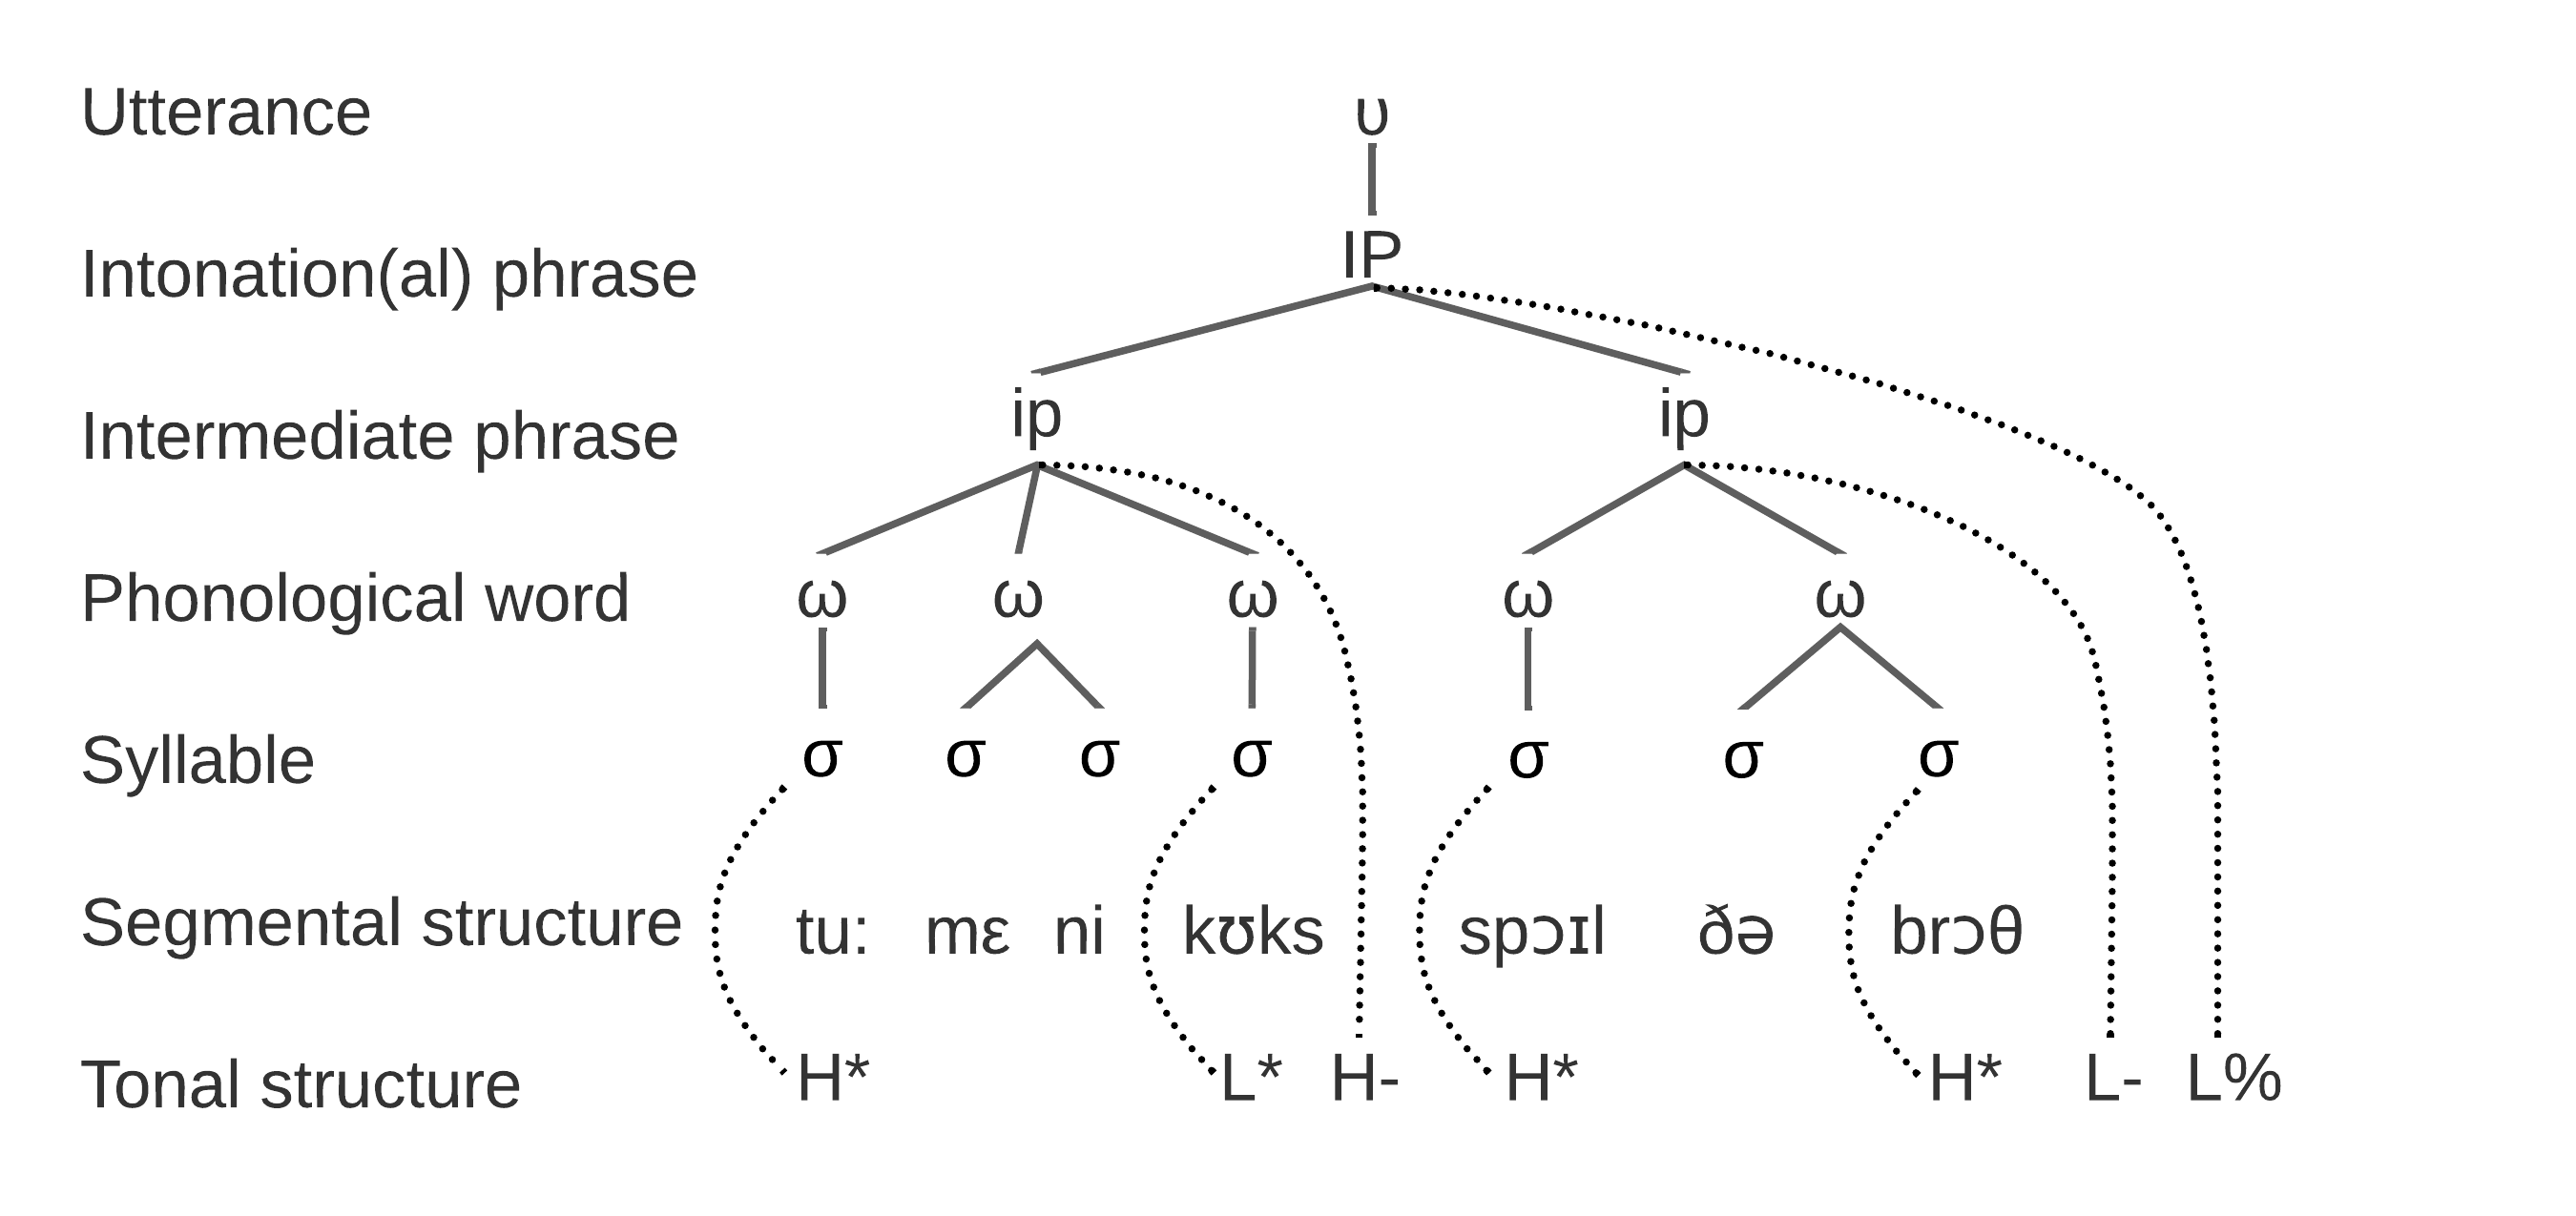
\includegraphics[scale = 0.5]{prosodic structure}
	\caption{Representation of a prosodic hierarchy, exemplified by the utterance ``Too many cooks spoil the broth", adapted from \citet[124]{gussenhovenPhonologyToneIntonation2004} following the reanalysis in \citet[781]{griceIntonation2006}.}
	\label{fig:prosodic_structure}
\end{figure}

In AM, pitch contours are described as sequences of tonal events. In West-Germanic languages, these tonal events encompass pitch accents and edge tones \citep[45]{laddIntonationalPhonology2008}. Intonational pitch accents (as opposed to lexical pitch accents, which occur, for example, in Swedish) are associated with a lexically stressed syllable and cue prominence in that syllable, while edge tones mark the edges of prosodic domains.\footnote{Note that insights from typologically diverse languages caution that assuming a one-to-one mapping between pitch accents and prominence on the one hand and edge tones and phrasing on the other may be too strict an assumption. \citet{griceAutosegmentalmetricalPhonologyUnpacking2022} discusses evidence from three languages that challenge this assumption: First, Tashlhiyt Berber exhibits high peaks that appear to cue prominence but are not associated with a prosodic head and can thus not be analyzed as pitch accents. Second, Maltese has high tones that are associated with a word edge instead of a head, yet also seem to cue prominence. Third, in Bari Italian, postfocal tones may be associated with a head but do not function as cues to prominence.} Between these tonal events, the pitch contour is merely ``transitioning" and thus phonologically unspecified \citep[44]{laddIntonationalPhonology2008}. This is in contrast to a basic assumption of IPO theory (short for \textit{Institute for Perception Research} in Eindhoven, where the IPO theory was advanced, \citealt{thartPerceptualStudyIntonation1990}), in which configurations of the pitch contour are specified that may stretch over several syllables \citep[12, 47]{laddIntonationalPhonology2008}. Tonal events in AM are phonologically specified as either High (H) or Low (L) tones, although the phonetic realization of these tones in terms of pitch scaling is dependent on many factors including emphasis or position in the sentence \citep[44]{laddIntonationalPhonology2008}. Pitch accents may consist of more than one tone and can thus be regarded as configurations, which partially reconciles AM and IPO theories \citep[62-64]{laddIntonationalPhonology2008}.

\begin{figure}
		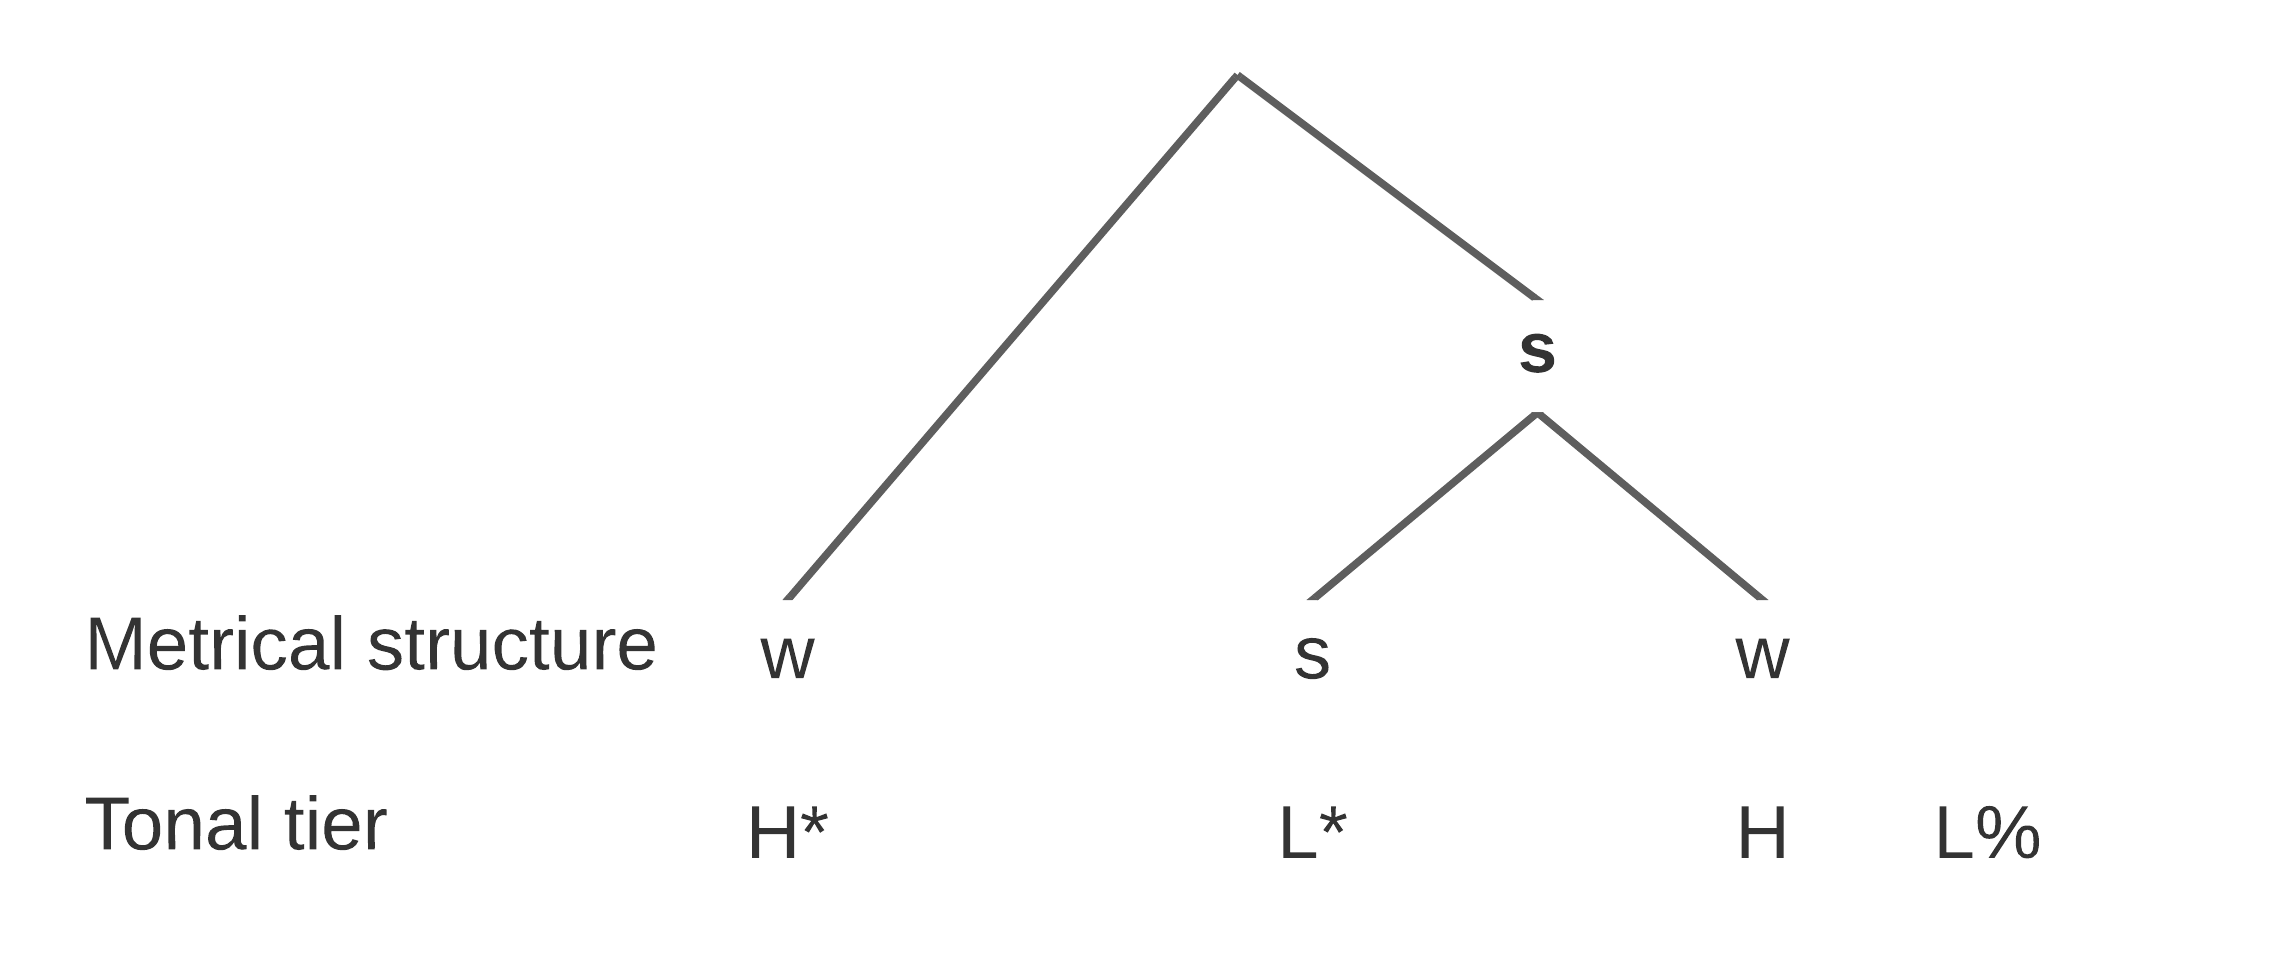
\includegraphics[scale = 0.5]{AM_example}
	\caption{Example of metrical structure and tonal tier in AM, adapted from \citet[284]{laddIntonationalPhonology2008}, representing the Eastern European Question Tune \citep{gricePlacePhraseAccents2000}.}
	\label{fig:AM_example}
\end{figure}

Pitch accents are a manifestation of metrical structure \citep[269]{laddIntonationalPhonology2008}. Metrical structure explicitly pertains to the relational aspect of prominence representing strength relations between the prosodic constituents of an utterance \citep[37]{arvanitiAutosegmentalMetricalModelIntonational2022}. Constituents are specified as strong or weak relative to each other (see Figure \ref{fig:AM_example}). Relationality is thus one of the pillars of AM theory. Crucially, metrical strength relations are understood as abstract and may manifest phonetically in different ways \citep[55-56]{laddIntonationalPhonology2008}. 

Metrical structure has been represented in forms of metrical trees \citep[e.g.,][]{libermanIntonationalSystemEnglish1975} or metrical grids \citep[e.g.,][]{selkirkPhonologySyntaxRelation1984}. In metrical trees, strength relations are represented as binary branching nodes that are labeled strong (s) or weak (w, see Figure \ref{fig:AM_example}). The nuclear accent is dominated exclusively by s-nodes, w-nodes to the left of the nucleus optionally carry a prenuclear accent, nodes to the right may be marked by postnuclear prominences \citep[3]{calhounCentralityMetricalStructure2010}. Metrical trees are by default right-branching, at least in West-Germanic languages, i.e., s-nodes normally occur to the right of w-nodes \citep{libermanIntonationalSystemEnglish1975, laddIntonationalPhonology2008}. Alternatively, in metrical grids, degrees of prominence are formalized in the number of beats assigned to a syllable with the most prominent syllable receiving a beat on a higher metrical level than other syllables \citep[15-16]{selkirkPhonologySyntaxRelation1984}. 

\largerpage
Regarding notation, some conventions have proven useful that are by now relatively widespread: Pitch accents are conventionally marked by stars or asterisks, in bitonal pitch accents, the central tone receives the star \citep[87]{laddIntonationalPhonology2008}. Edge tones can be distinguished by the strength of the prosodic boundary they are associated with. In English, phrase accents (H- or L-) are assumed to mark the end of an intermediate phrase (ip), while boundary tones (H\% and L\%) mark the end of an intonation phrase (IP, \citealt{pierrehumbertPhonologyPhoneticsEnglish1980, beckmanIntonationalStructureJapanese1986}). These conventions are largely followed in AM-based analyses of German intonation \citep[e.g.,][]{feryGermanIntonationalPatterns1993, griceGermanIntonationAutosegmentalMetrical2005}.\footnote{One difference relates to the use of the term \textit{phrase accent}. While in the early American English AM analyses, phrase accents were simply understood as tones marking the boundaries of intermediate phrases, the German system distinguishes between phrase accents that are associated with a postnuclear prominence and phrase tones that mark ip boundaries \citep{griceIntonationLautspracheTonale2016}.} 

Based on Pierrehumbert's \citeyearpar{pierrehumbertPhonologyPhoneticsEnglish1980} work and thereby rooted in the AM tradition, the ToBI (Tones and Breaks Indices) transcription system was introduced by \citet{silvermanTOBIStandardLabeling1992} as an attempt to standardize prosodic annotation. This initiative sprouted many more ToBI systems for a diverse set of languages, among them GToBI for German intonation analysis \citep{griceGermanIntonationAutosegmentalMetrical2005}. GToBI assumes six basic pitch accent types, namely a peak accent H*, a rise from low to peak L+H*, a low accent L*, a valley accent plus rise L*+H, a step-down from high to low H+L*, and a step-down from high to mid H+!H*. Intermediate phrase boundaries are marked by H- or L- tones, intonation phrases additionally by L\% or H\% tones. H tones within pitch accents or boundary tones may also undergo upstep (marked by \textasciicircum) or downstep (marked by !, \citealt[see][67-69 for details]{griceGermanIntonationAutosegmentalMetrical2005}). Break indices, which are used in ToBI annotations to mark boundary strength, play a subordinate role in the GToBI system. In the original ToBI system, four levels of break indices were distinguished, which correspond to very close inter-word junctures (1), phrase-internal word boundaries (2), intermediate phrase boundaries (3), and intonation phrase boundaries (4) \citep{silvermanTOBIStandardLabeling1992, beckmanOriginalToBiSystem2005}. In GToBI, the break indices 3 and 4 still correspond to intermediate and intonation phrase boundaries respectively, however, these break indices are not explicitly annotated beyond the marking of phrase accents and edge tones with the - and \% diacritics. In addition, rhythmic and tonal breaks may be annotated with 2r and 2t respectively to indicate mismatches between tonal and rhythmic structure \citep{griceGermanIntonationAutosegmentalMetrical2005}.

ToBI labeling systems are at their core phonological. From a theoretical perspective, this means that they come with inherent assumptions, e.g., regarding the pitch accent inventory. From a practical side, this can pose difficulties to transcribers, who struggle to make the appropriate phonological abstractions. Theoretical assumptions underlying the ToBI system have been called into question numerous times. For instance, it is a much disputed issue whether L+H* and H* pitch accents should be regarded as two distinct phonological categories or two phonetic realizations of the same category \citep[e.g.,][]{laddIntonationalPhonology2008, arvanitiDisentanglingEmphasisPragmatic2022, laddTroubleToBI2022}. By contrast, there are also suggestions to expand the pitch accent inventory, specifically for German by including an (LH)* accent that phonetically sits between L+H* and L*+H accents (\citealt{zahner-ritterThreeKindsRisingFalling2022}, see also Section \ref{sec:background_F0} for a brief overview of the ``on-ramp versus off-ramp" debate). To resolve practical issues, other labeling systems have been introduced that at least notationally follow the same (AM) tradition but are more phonetic in nature and thus less theoretically loaded. One example is the DIMA annotation system (short for \textit{Deutsche Intonation – Modellierung und Annotation}), which nevertheless adheres to some of the same principles and conventions used in ToBI systems \citep{kuglerDeutscheIntonationModellierung2022}. Similar to these systems, DIMA includes a tonal and a phrasal tier, however, additionally, there is a prominence tier, which allows for the impressionistic annotation of prominence levels independently from the other two tiers. Crucially, DIMA is easier to use for annotators because they need not make phonological abstractions. Nevertheless, DIMA labels are easily translatable into other systems, such as GToBI. 

Specifically, DIMA allows for two types of phrase boundaries to be distinguished, strong (\%) and weak (-). This is similar to GToBI, however, it is cautioned that in DIMA, these boundary types are not directly related to intermediate and intonational phrases in order to remain relatively theory neutral \citep[29]{kuglerDeutscheIntonationModellierung2022}. In terms of tonal annotations, DIMA sticks to the distinction between L and H tones,  allowing especially the H tones to be modified via downstep (!) or upstep (\textasciicircum), similar to GToBI. Three types of tones are distinguished: edge tones, accentual tones, and non-accentual tones. Edge tones mark boundaries, accentual tones are associated with a prominent syllable and marked with a star/an asterisk, and non-accentual tones are turning points that are not prominence-cueing \citep[38]{kuglerDeutscheIntonationModellierung2022}. A difference to GToBI is the treatment of complex labels, such as bitonal pitch accents, which are broken up into their phonetic components, so that each individual label is monotonal. Finally, DIMA adds the prominence tier: Permitted labels are \textit{weak} (1), indicating that a prominent syllable is not necessarily accompanied by F0 movement, \textit{strong} (2), which is typically associated with full pitch accents, and \textit{extra strong} (3), which is used for emphatic realizations of full pitch accents \citep[34]{kuglerDeutscheIntonationModellierung2022}.

Pitch accents, by way of occurring in metrically strong positions, act as a cue to prominence \citep[54]{laddIntonationalPhonology2008}. In addition, multiple continuous measures of the phonetic signal have been investigated as potential correlates of prominence, which are not just related to the pitch contour but also to duration and intensity. The following section summarizes some of the most pervasive findings in this line of research.

\subsection{Acoustic correlates of prominence} \label{section: acoustics}

Prosodic prominence is multidimensional, as it is encoded by a variety of cues related to changes in the fundamental frequency (F0), duration, intensity, and spectral characteristics of the speech signal \citep[e.g.,][]{baumannWhatMakesWord2018, fryDurationIntensityPhysical1955, kochanskiLoudnessPredictsProminence2005, liebermanAcousticCorrelatesWord1960, roessigTracingPhoneticSpace2022, sluijterSpectralBalanceAcoustic1996}. Perceptually, these acoustic cues correspond to pitch, length, and loudness. Generally, prosodically prominent entities are produced with steeper and more rising F0 contours, longer duration, and higher intensity than less prominent entities, at least in West-Germanic languages. There are multiple ways of quantifying each of these acoustic dimensions and since the choice of parameters to be taken as correlates of prominence is crucial for the identification and analysis of individual differences, this section is dedicated to a detailed discussion of the acoustic form of prosodic prominence. The section is divided into the subsections Intonation (\ref{sec:background_F0}), dealing primarily with fundamental frequency, and Timing (\ref{section: timing}), which is concerned with duration and intensity.

\subsubsection{Intonation} \label{sec:background_F0}

Fundamental frequency (F0) has often proven to be the most important correlate of prominence at the phrase-level in West-Germanic languages in general \citep{bolingerTheoryPitchAccent1958, fryExperimentsPerceptionStress1958, liebermanAcousticCorrelatesWord1960, thartPerceptualStudyIntonation1990, bishopPhonologyPhoneticsSignalextrinsic2020, severijnenYourVOORnaamNot2024} and in German in particular \citep{arnoldUsingGeneralizedAdditive2013, niebuhrRelativeCueingPower2017, baumannWhatMakesWord2018, roessigTracingPhoneticSpace2022}. Three characteristics defining the F0 space have been shown to affect (the perceived degree of) prosodic prominence of a syllable or word, namely, (1) the direction of F0 movement, where rising contours are more prominent than falling ones \citep{baumannImportanceTonalCues2014, baumannPerceptualProminencePitch2015}, (2) the height or scaling of the F0 peak, where a higher peak or larger excursion is more prominent than a lower peak \citep{rietveldRelationPitchExcursion1985, laddPerceptionIntonationalEmphasis1997, knightShapeNuclearFalls2008,  baumannPerceptualProminencePitch2015}, and (3) the alignment of the F0 peak with the metrically strong syllable, where a later alignment is more prominent than an earlier one \citep{laddPerceptionIntonationalEmphasis1997, kohlerTimingCommunicativeFunctions2005, niebuhrPerzeptionUndKognitive2007}. 

Numerous operationalizations have been suggested to categorize or quantify these characteristics of the F0 contour. While it is rather straightforward to determine the direction of F0 movement, which can only ever be rising, falling or level, there are substantial methodological differences in capturing the extent of the rise or fall, i.e., F0 scaling as well as alignment, which are intertwined with underlying theoretical considerations. Major differences between such operationalizations are whether they take a categorical or a continuous approach, whether they rely on annotated landmarks, such as F0 minima or maxima and turning points, or derive directly from the (weighted) signal and whether they combine several of the aforementioned F0 characteristics or single out only one of them.

One popular approach to categorizing the F0 contour, especially the part that aligns with metrically strong syllables, is via the aforementioned prosodic annotation schemes ToBI for American English \citep{silvermanTOBIStandardLabeling1992,beckmanOriginalToBiSystem2005} and GToBI for German \citep{griceConsistencyTranscriptionLabelling1996, griceDeutscheIntonationUnd2002}. Pitch accents defined as ``pitch movements or configurations that lend prominence to their associated word" \citep[868]{silvermanTOBIStandardLabeling1992} can be understood as bundles of acoustic cues that are identified and labeled as they are perceived by a listener (i.e., the annotator). Classifying the type of pitch accent requires consideration of direction of movement (e.g., L+H* marks a rising accent, H+!H* a falling one), scaling (L* is defined as a low accent, H* as a high accent), and alignment (L*+H describes a low target on the accented syllable followed by a rise, L+H* indicates that a high target is already reached within the accented syllable, \citealt[see][]{griceGermanIntonationAutosegmentalMetrical2005}). Since the annotator bases their decision on a holistic impression of the signal, such categorizations involve the perception of changes in duration or intensity in addition to pitch. The GToBI guidelines even explicitly note that intensity and duration may be decisive when annotating L* accents \citep[278]{baumannImportanceTonalCues2014, griceDeutscheIntonationUnd2002} as the difference between an L* accented and an unaccented syllable may be one of perceived length and loudness in the absence of a noticeable pitch movement. 

While the presence of a pitch accent already indicates higher prominence relative to a lack of pitch accent, accent types can further be ordered by their (perceived) degree of prominence. \citet{baumannPerceptualProminencePitch2015} showed that for German, the following hierarchy in terms of perceived prominence (left to right from most prominent to least prominent) emerges: 

\hspace*{20mm}L+H* > L*+H > H* > H+!H* > H+L* > !H* > L*

What becomes apparent from this ranking is that the direction of pitch movement is most important for the perception of prominence, with rising contours being judged as more prominent than falling ones. However, scaling also plays a role, both in absolute terms, in that high accents are more prominent than low accents and considering more dynamic changes, in that accents including larger pitch movement (e.g., H+!H* and H+L*) are more prominent than relatively level accents (e.g., !H* and L*). \citet{baumannWhatMakesWord2018} confirm these findings albeit using broader accent type categories, with rising accent types being judged as most prominent followed by high, falling, and low accents, respectively. A similar ranking of accent types in terms of perceived prominence was established by \citet{bishopPhonologyPhoneticsSignalextrinsic2020} for American English.
 
When considering accent type as a correlate of prosodic prominence, it comes as no surprise that a variable involving several acoustic dimensions is a more robust correlate of prominence than an isolated cue, such as mean or maximum F0. \citet{baumannWhatMakesWord2018} showed that categorical prosodic variables, e.g., accentedness (i.e., the presence or absence of a pitch accent) and type of pitch accent, were more predictive of perceived prominence than continuous variables. A similar conclusion is reached by \citet{bishopPhonologyPhoneticsSignalextrinsic2020}. However, there is some criticism surrounding the ToBI system in particular (see Section \ref{section: structural prominence} for some arguments) and the use of categorizations of the pitch contour in general. For example, \citet{griceIntegratingDiscretenessContinuity2017} investigating continuous and categorical prosodic correlates of different focus types in German found that although not all speakers make categorical distinctions in terms of pitch accent type between different focus types, listeners are still able to derive the correct intended function. They conclude that ``discrete pitch accent categories are only a poor approximation for how listeners comprehend intended pragmatic meanings" \citep[101, see Section \ref{section: Information structure} for a more detailed discussion of the prosodic encoding of meaning contrasts]{griceIntegratingDiscretenessContinuity2017}. In a similar vein, \citet{laddTroubleToBI2022} cautions that overly relying on categories may result in the neglect of meaningful gradient variation. 

This issue is immediately relevant to the present book as coarse-grained categorization may also gloss over individual variability. For example, \citet{niebuhrAreThereShapers2011} observed that German speakers differed in whether they relied on F0 shape or alignment in order to distinguish between H* and H+L* accents. In order to arrive at a better understanding of the nature of individual variability, it is thus necessary to consider gradience in the prosodic signal by looking at continuous operationalizations of acoustic parameters.

Theoretical assumptions shaping prosodic classification systems also have implications for considerations regarding continuous measures. One major point of contention has been the on-ramp versus off-ramp debate \citep[see][]{gussenhovenPhonologyToneIntonation2004, ritterRoleTonalOnglides2015, barnesRampsIntonationalPhonology2021}. In an on-ramp approach, the nuclear tone and the movement \textit{towards} it are considered most important for the interpretation of an F0 contour, while conversely, in an off-ramp model, the nuclear tone and the movement \textit{away from} it are considered decisive. Systems devised in the tradition of the British school are considered off-ramp approaches \citep[e.g.,][]{gussenhovenTranscriptionDutchIntonation2005, petersPhonologicalSemanticAspects2018}, ToBI annotation systems, such as the classic Mainstream American English ToBI \citep{silvermanTOBIStandardLabeling1992,beckmanOriginalToBiSystem2005} and the German GToBI \citep{griceConsistencyTranscriptionLabelling1996, griceDeutscheIntonationUnd2002}, can be regarded as predominantly on-ramp approaches. However, such classifications are not completely definitive as, for instance, the GToBI inventory also includes an L*+H accent, which describes a pitch accent in terms of its nuclear and trailing tone. When quantifying the F0 curve in a continuous measure, for example with regard to excursion size, one similarly has to make the theoretical decision whether to consider the tonal onglide, the offglide, or both. There is, in fact, empirical evidence to support both approaches. In a perception study, \citet{ritterRoleTonalOnglides2015} found that German listeners were able to make use of tonal onglide in order to determine if an utterance contained given/non-contrastive or new/contrastive information. Similarly, \citet{braunPrenuclearActivatesAlternatives2019} found that the F0 contour leading up to and including the accented syllable was particularly important for German listeners' interpretation of utterances with regard to their contrastiveness. In contrast, \citet{barnesRampsIntonationalPhonology2021} found that American English listeners relied on tonal onglide and offglide to an almost equal extent, at least when it comes to tonal events ranging from contours typically defined as H+!H* to L+H*. However, when looking at a continuum of values typical of L*+H to L+H* accents, the shape of the fall seemed to matter much less than the shape of the rise. Taken together, these findings suggest that it may be more important to account for the on-ramp in order to accurately describe prosodic prominence.

Oftentimes, continuous measures rely on (annotated) landmarks or turning points in the F0 contour or average across certain parts of the signal. Such measures can be quite successful at capturing prominence, for example, in \citet{roessigTracingPhoneticSpace2022}, where only continuous parameters were considered, mean F0 was the most important correlate to distinguish accented from unaccented words, outperforming measures accounting for aspects of duration, intensity, formant values, and articulatory gestures. However, concerns have been raised that these landmarks determined by the peaks and elbows in the continuous F0 trajectory may not accurately reflect perceptual reality \citep{albertModelSonorityBased2023} and that static parameters calculated from these landmarks (e.g., peak alignment, pitch excursion, or tonal onglide) may conceal more fine-grained information, such as pitch accent shape \citep{barnesTonalCenterGravity2012}. To address these issues, more sophisticated measures have recently been proposed. 

One such measure of F0, which takes into account both the shape of the rise and the shape of the fall of an accent and thus also unifies on-ramp and off-ramp approaches, is the Tonal Center of Gravity (TCoG, \citealt[see][]{barnesTonalCenterGravity2012, barnesRampsIntonationalPhonology2021}). The TCoG measures represent an alternative to traditional measures that are reliant on turning points and are able to capture both alignment in time and F0 scaling (see Figure \ref{fig:TCoG}). TCoG alignment (or TCoG-t) constitutes a point in time relative to the beginning of the target domain weighted by the F0 contour. Values of TCoG alignment are higher the later a rise occurs and the more \textit{scooped} the F0 contour. Conversely, values are lower the earlier the rise and the more \textit{domed} the F0 shape. TCoG alignment thus more closely captures \textit{perceived} alignment, which is not only influenced by actual peak alignment but also by the shape of the F0 movement surrounding the peak \citep{barnesTonalCenterGravity2012}. TCoG scaling (or TCoG-f) is measured as the weighted average F0 over the target domain. Crucially, more sonorous regions contribute more to the value of TCoG scaling, as it is assumed that F0 in these regions is more salient to the listener \citep{barnesSegmentalInfluencesPerception2014}. 

\begin{figure}
		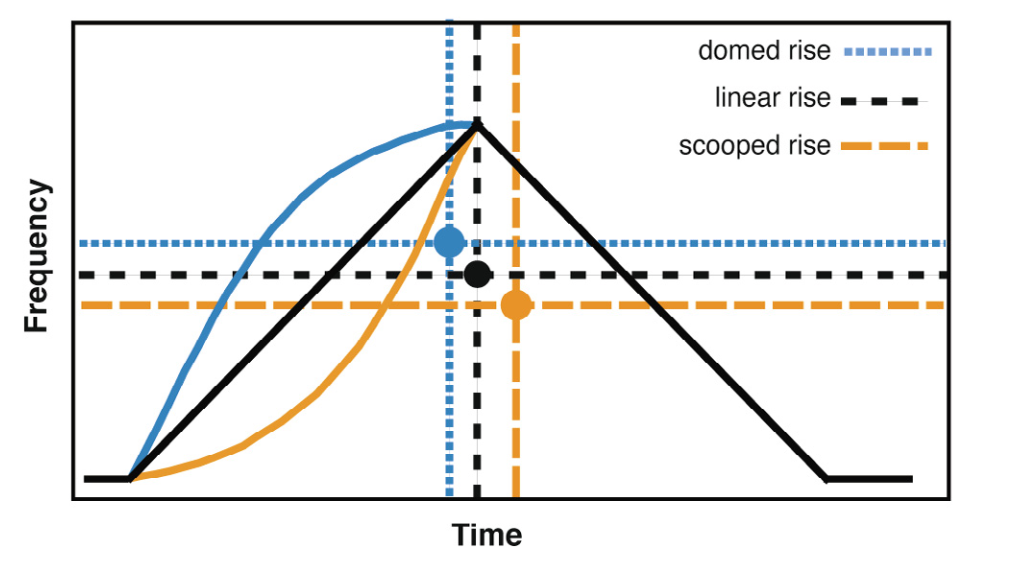
\includegraphics[scale = 0.2]{TCoG}
	\caption{Schematization of TCoG alignment and scaling \citep[6]{barnesRampsIntonationalPhonology2021}. A \textit{domed} F0 contour leads to an earlier and higher TCoG (colored circles), a \textit{scooped} contour to a later and lower TCoG.}
	\label{fig:TCoG}
\end{figure}

TCoG measures thus quantify information about the F0 contour shape that is not captured by traditional measures of scaling and alignment and has been shown to more accurately describe prosodic phenomena in some studies. For instance, TCoG alignment more robustly distinguished between L*+H and L+H* pitch accents in American English productions than traditional turning point alignment values \citep{barnesTonalCenterGravity2012}. Results from a study by \citet{bruggemanUnifyingSpeakerVariability2017} also favor TCoG (alignment) over turning point based measures of alignment and scaling, as the former yields a more unified picture of focus type marking in Egyptian Arabic across different speakers. Analogously to traditional measures of alignment and scaling, a higher TCoG alignment value (i.e., later alignment of the bulk of the F0 contour) and higher TCoG scaling is assumed to correlate with a higher degree of prominence. 

Another recent suite of prosodic measurements, which was partly inspired by \citeauthor{barnesTonalCenterGravity2012}'s \citeyearpar{barnesTonalCenterGravity2012} Tonal Center of Gravity, comes from the ProPer toolbox \citep{albertUsingPeriodicEnergy2018, albertModelSonorityBased2023}. ProPer stands for PROsodic analysis with PERiodic energy and has its origins in research on sonority \citep{albertModelSonorityBased2023}. Periodic energy, which is the log transform of the acoustic power in the periodic parts of the signal (see \citealt[143-145]{albertModelSonorityBased2023} for details), is taken as the acoustic correlate of sonority. Fluctuations in the periodic energy curve thus correlate systematically with syllable boundaries. Perceptually, periodic energy also links to pitch intelligibility \citep[55-56]{albertModelSonorityBased2023}, which is presumably enhanced in portions of the signal produced with higher periodic energy (see Figure \ref{fig:proper_simple}). ProPer thus combines several acoustic dimensions to derive acoustic measurements that are firmly grounded in perceptual reality, making it the most suitable toolbox for the present investigation. 

\begin{figure}
		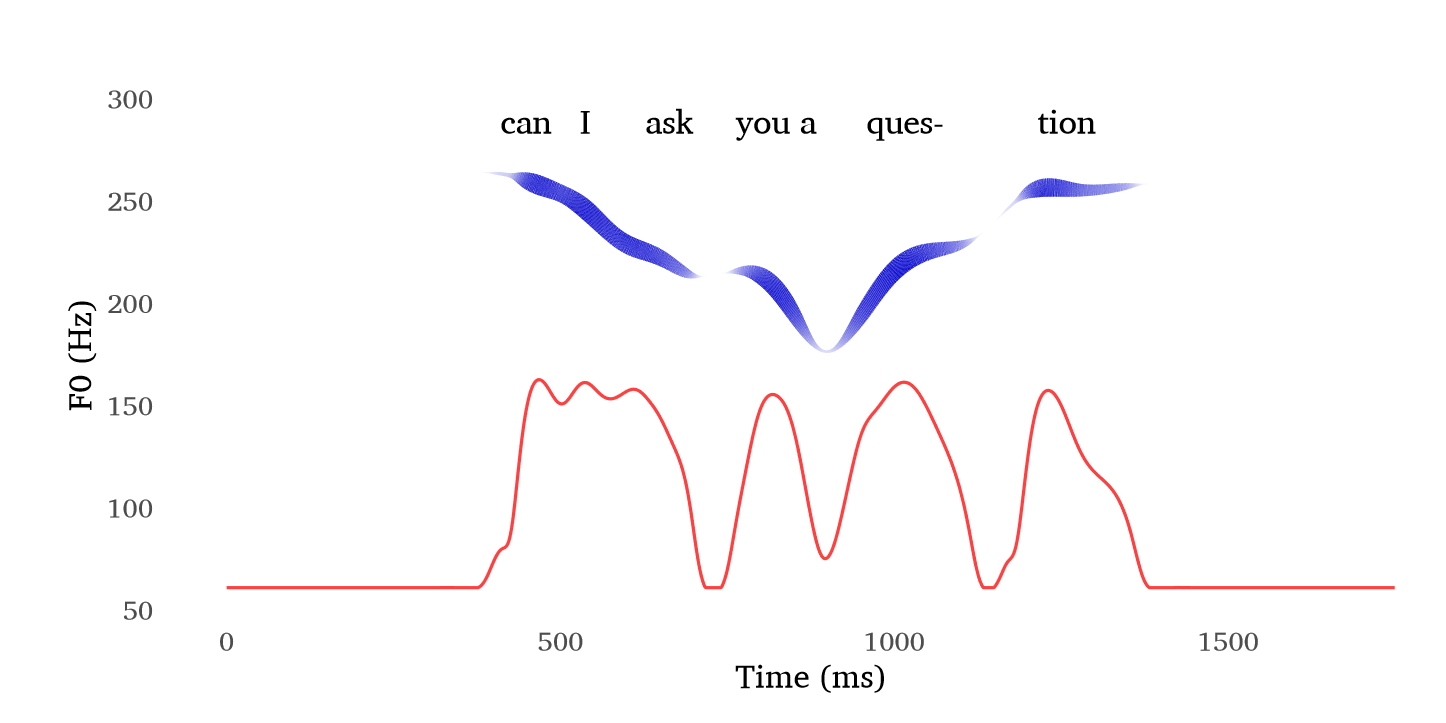
\includegraphics[scale = 0.2]{proper}
	\caption{Schematization of the relation between F0 curve (blue) and periodic energy (red), i.e., a ``periogram" \citep[153]{albertModelSonorityBased2023}. Note that the F0 curve is enhanced by periodic energy, that is, it is thicker in areas with higher periodic energy as indicated by the red curve. The y-axis on the left corresponds only to the F0 curve, not to periodic energy.}
	\label{fig:proper_simple}
\end{figure}

Based on the periodic energy curve (Figure \ref{fig:proper_simple}, red line) and the F0 curve modulated by periodic energy (Figure \ref{fig:proper_simple}, blue line), a number of prosodic variables can be computed, which correspond to cues that are traditionally assumed to correlate with prosodic prominence, such as F0 alignment and scaling. Methodologically, similar to TCoG, this has the advantage that there is no need for prior labeling of turning points. Instead, points of interest are directly computed from the signal. Specifically, for each syllable, a Center of Mass (CoM) and a Center of Gravity (CoG) can be determined. The CoM is the point in time that splits the area under the periodic energy curve of a syllable into two equal parts. Measuring the F0 at the CoM yields a robust representation of perceived peak height, which roughly corresponds to TCoG scaling (TCoG-f). A Delta F0 value can be calculated by measuring the F0 at the CoM of two subsequent syllables and taking their difference. Delta F0 thus constitutes a measure of the extent and direction of F0 change across syllables, which can be interpreted similarly to tonal onglide or tonal offglide, depending on which syllables are being compared. Analogous to the TCoG by \citet{barnesTonalCenterGravity2012, barnesRampsIntonationalPhonology2021}, in the ProPer framework, a Center of Gravity (CoG) is computed as an averaged point in time weighted by the F0 curve multiplied by periodic energy. CoG can thus be used as a measure replacing traditional F0 peak alignment or TCoG alignment. Relating the distance between the CoM and the CoG yields another ProPer measure, namely synchrony. Synchrony accounts for the extent and direction of F0 change within one syllable as well as the contour's shape. If the CoG is located to the right of the CoM (reflected in a positive synchrony value), F0 is rising within the syllable, if the CoG occurs to the left of the CoM (synchrony is negative), F0 is falling. If CoG and CoM are perfectly aligned (i.e., synchrony has a value of 0), the F0 contour is either level or exhibits a symmetrical rise-fall or fall-rise.

Although initially designed for the study of sonority, ProPer measures have proven useful in quantifying prominence phenomena as well \citep{roessigTracingPhoneticSpace2022, sbrannaProsodicMarkingInformation2023}. For example, \citet{roessigTracingPhoneticSpace2022} found synchrony to successfully distinguish broad from narrow and contrastive focus domains as well as narrow from contrastive focus in German, with higher synchrony indicating higher prominence.

\subsubsection{Timing} \label{section: timing}

Further gradient prosodic cues capturing the acoustic dimensions of duration and intensity have been found to be related to prominence in production and perception. These are jointly considered here under the notion of timing, since both dimensions contribute to a perception of rhythm in speech \citep[cf.][]{albertRhythmTimescale2024}. Numerous studies have shown that more prominent units are produced with longer duration and higher intensity than less prominent units and that longer and louder units are perceived as being more prominent (e.g., \citealt{fryDurationIntensityPhysical1955, beckmanStressNonStressAccent1986, aylettSmoothSignalRedundancy2004,  coleSoundStructureMeaning2019}). In terms of a ranking of prominence correlates, Fry's \citeyearpar{fryDurationIntensityPhysical1955, fryExperimentsPerceptionStress1958} perceptual studies suggest that duration ranks higher than intensity but lower than F0 in cueing prominence for American English listeners. Similarly, \citet{turkProcessingDurationIntensity1996} find duration to be more important to the perception of prominence and intensity independent of duration to contribute little to the perception of prominence. However, in their production study on German, \citet{roessigTracingPhoneticSpace2022} find that intensity (measured as RMS amplitude) is more successful than vowel duration in distinguishing accented from unaccented words. Intensity is also found a better predictor to prominence than duration in \citet{liebermanAcousticCorrelatesWord1960} and \citet{kochanskiLoudnessPredictsProminence2005}. These differences may stem from different manipulations of the speech material under investigation or from different operationalizations of the duration and intensity measures.

Measuring duration is primarily a matter of determining segmental boundaries, but studies differ in which domain they consider for their duration measurement. Common choices (all including the syllablic nucleus) are the vowel \citep[e.g.,][]{fryDurationIntensityPhysical1955, beckmanStressNonStressAccent1986, turnbullListenerorientedPhoneticReduction2019, roessigTracingPhoneticSpace2022}, the syllable \citep[e.g.,][]{aylettSmoothSignalRedundancy2004, baumannTonalArticulatoryMarking2007, muckeEffectFocusMarking2014}, the foot \citep{baumannTonalArticulatoryMarking2007, muckeEffectFocusMarking2014}, and the word \citep[e.g.,][]{bakerVariabilityWordDuration2009, breenAcousticCorrelatesInformation2010, coleSoundStructureMeaning2019, turnbullListenerorientedPhoneticReduction2019}. In \citet{muckeEffectFocusMarking2014}, syllable and foot (which is equivalent to the word domain in their study) duration are similarly effective in distinguishing between different focus types. \citet{baumannTonalArticulatoryMarking2007}, however, found that focus types may be more robustly encoded in the duration of the foot than that of the syllable. \citet{turnbullListenerorientedPhoneticReduction2019} observed that unpredictability is marked by both longer vowel duration and longer word duration, but that individual speakers differed in the extent to which they manipulated these two variables. The question of which duration measure is optimal to capture prominence effects is thus not yet conclusively determined and it may be beneficial to consider duration over both a smaller domain (such as the syllable) and a larger domain (such as the word).

Intensity can also be quantified in various ways. Traditionally, studies consider either peak or mean overall intensity \citep[e.g.,][]{fryDurationIntensityPhysical1955} measured as the sound pressure level or RMS amplitude over the full spectrum. However, since the seminal study by \citet{sluijterSpectralBalanceAcoustic1996}, newer measures have gained popularity that calculate the intensity in or intensity ratios across parts of the spectrum, i.e., the spectral emphasis, spectral balance or spectral tilt/slope. This approach is motivated by the perceptual correlate of intensity, which is loudness. \citet{sluijterSpectralBalanceAcoustic1996} argue that intensity in lower frequencies (up to 500 Hz) contribute less to perceived loudness than intensity in higher frequencies. Indeed, \citet{sluijterSpectralBalanceAcoustic1996} found that what they call spectral balance is a better correlate of lexical stress than intensity. Although the study by \citet{sluijterSpectralBalanceAcoustic1996} was concerned with the acoustic correlates of lexical stress, this relation between spectral balance and loudness should generally hold true and thus extend to phrase-level prominence. In fact, \citet{heldnerSpectralEmphasisAdditional2001} found spectral emphasis to outperform overall intensity in classifying phrase-level accent in Swedish.

However, in contrast to findings by \citet{sluijterSpectralBalanceAcoustic1996} and \citet{heldnerSpectralEmphasisAdditional2001}, \citet{kochanskiLoudnessPredictsProminence2005} in their study using classifiers trained on human prominence judgments found that overall intensity by far outperformed spectral slope in distinguishing prominent from non-prominent syllables. Such differing findings may again arise from different operationalizations. As already apparent from the terminological chaos, there are many ways to measure spectral emphasis, slope, balance or tilt. \citet{heldnerReliabilityOverallIntensity2003} provides a brief overview of different measures and terminology. He suggests a broad binary distinction between spectral tilt and spectral emphasis, the former measuring the slope of the spectrum and the latter relative energy in higher-frequency bands \citep[40]{heldnerReliabilityOverallIntensity2003}. However, within these two categories, several more fine-grained distinctions can be made and there is no consensus on the best way to obtain these measures. In summary, it seems that spectral balance and spectral emphasis are not (much) more successful in capturing prominence at a phrasal level than overall intensity \citep{sluijterSpectralBalanceAcoustic1996, heldnerSpectralEmphasisAdditional2001, kochanskiLoudnessPredictsProminence2005}, which is also easier to obtain. 

Some research suggests that duration and intensity may be processed together \citep[e.g.,][]{turkProcessingDurationIntensity1996}. This justifies a measure combining these two acoustic dimensions, such as periodic energy mass \citep{albertModelSonorityBased2023}. Periodic energy mass quantifies the area under the periodic energy curve within an interval, i.e., the syllable. It is the integral of duration and power. \citet{roessigTracingPhoneticSpace2022} found periodic energy mass to be among the most important prosodic cues to distinguish accented from unaccented words. Similarly, in \citet{sbrannaProsodicMarkingInformation2023}, periodic energy mass was the most important correlate of marking information status in Italian.

To summarize, prosodic prominence relates to multiple acoustic dimensions that can each be measured or categorized in various ways, which has implications for findings regarding their robustness and strength. The present book draws from categorical and continuous approaches to prosody, while reducing the number of prosodic parameters under consideration to a reasonable number (see Sections \ref{section: measurements study1} and \ref{section: measurements study2} for details). The following sections will now explore prosodic prominence from a functional perspective.

\section{Information structure and prosodic prominence} \label{section: Information structure}

One of the functions of prosodic prominence is marking information structural categories, such as focus and information status. Information structure encompasses several theoretical concepts, such as the distinctions between focus and background, theme and rheme, topic and comment, as well as givenness and newness. \citet[199]{hallidayNotesTransitivityTheme1967} defines information structure as ``the relation of what is being said to what has gone before in the discourse" and the ``internal organization [of a clause] into an act of communication." Information structure is thus related to the communicative function of managing common ground \citep[e.g.,][]{krifkaBasicNotionsInformation2008}. This chapter will unpack the notions of focus and givenness (or information status) and their relation to prosodic prominence. The latter are discussed with regard to West-Germanic languages in particular, as the mapping of prosody to information structure is far from universal and other languages may rely predominantly on non-prosodic factors, such as word order or morphological focus particles \citep[e.g.,][]{buringTypologyFocusRealization2009}. As far as information structural categories are concerned, information status is the primary interest of the present book. However, since focus is intricately linked with information status and much prosodic research has been dedicated to the study of focus marking, the following sections will introduce and attempt to disambiguate both concepts. 

\subsection{Focus} \label{sec: focus background}

One of the most important information structural categories is that of focus. \citet[204]{hallidayNotesTransitivityTheme1967} suggests that information \textit{in focus} is presented by the speaker ``as not being recoverable from the preceding discourse." Similarly, \citet[448]{buringSemanticsIntonationInformation2007} argues that focus occurs in conjunction with the most informative part of a sentence. \textit{Background} is generally used as a complementary notion to focus: What is not in focus is in the background. A well-established idea of focus from the theory of Alternative Semantics defines focus by its property of introducing a set of alternatives \citep{roothTheoryFocusInterpretation1992}. These alternatives are relevant for the interpretation of the focused expression \citep[see also][]{krifkaBasicNotionsInformation2008}. In example \ref{itm:Mona}, the focused entity is ``Mona", marked by square brackets and a subscript \textsubscript{F}. The expression ``Mona" induces a set of alternatives, i.e., people who broke their arm. ``Mona" also corresponds to the wh-expression in the preceding question. This correspondence is known as Question-Answer Congruence and can serve as a tool to identify the focus domain \citep[e.g.,][]{buringSemanticsIntonationInformation2007}. 

\begin{enumerate}[label=(\arabic*)]
\item \label{itm:Mona} Who broke their arm?\newline[MOna]\textsubscript{F} broke her arm.
\end{enumerate}

Focused parts of an utterance are prosodically emphasized, i.e., produced with a pitch accent \citep[e.g.,][]{hallidayNotesTransitivityTheme1967, cutlerSemanticFocusSentence1979}. Specifically, the nuclear accent has a special role in signaling focus \citep[257, 259]{laddIntonationalPhonology2008}. In example \ref{itm:Mona} above, the nuclear accent falls on the first syllable of ``Mona" (as signaled by capitalization) marking ``Mona" as the focused constituent, while the rest of the sentence is deaccented and in the background. Under the Focus-to-Accent approach \citep[e.g.,][]{hallidayNotesTransitivityTheme1967, gussenhovenFocusModeNucleus1983, selkirkPhonologySyntaxRelation1984}, the location of the nuclear accent follows logically from language-specific rules once the focus domain is known. Conversely, the location of the nucleus indicates which constituent is in focus. However, it is not necessarily just the pitch accented constituent that is in focus. In the case of broad focus, the pitch accent is assumed to \textit{project} focus onto a larger prosodic constituent as in example \ref{itm:house}, where the focus domain encompasses the complete sentence \citep{selkirkPhonologySyntaxRelation1984, selkirkSentenceProsodyIntonation1995}. The constituent receiving the nuclear accent, e.g., ``house" in the present example, is the focus exponent \citep{laddIntonationalPhonology2008}.

\begin{enumerate}[resume*]
\item \label{itm:house} What happened?\newline
[Lola sold her HOUSE.]\textsubscript{F}
\end{enumerate}

Types of focus can thus be distinguished by their scope: Example \ref{itm:Mona} is an instance of narrow focus, example \ref{itm:house} represents broad focus. Additionally, focus has been classified by the degree of contrastiveness that is evoked \citep{laddStructureIntonationalMeaning1980, laddIntonationalPhonology2008}. \citet{calhounCentralityMetricalStructure2010} following \citet{bolingerFormsEnglishAccent1965} argues that all focused entities induce some contrast by way of introducing a set of alternatives. The degree of contrastiveness is a matter of the restrictedness of the number of alternatives \citep[8]{calhounCentralityMetricalStructure2010}. In broad focus, the set of alternatives is not clearly defined \citep[8]{calhounCentralityMetricalStructure2010}. The highest degree of contrastiveness is induced in corrective focus \citep{gussenhovenPhonologyToneIntonation2004}, where the focused constituent presents a direct alternative to a previously established entity as in example \ref{itm:horse}, where ``house" contrasts with ``horse".

\begin{enumerate}[resume*]
\item \label{itm:horse} Did Lola sell her horse?\\
Lola sold her [HOUSE.]\textsubscript{F}
\end{enumerate}

The relation between focus (types) and prosodic prominence in West-Germa\-nic languages has received much attention in recent research \citep[e.g.,][]{feryPitchAccentScaling2008, muckeEffectFocusMarking2014, roessigTracingPhoneticSpace2022}. Studies have identified both categorical and continuous correlates of focus in addition to accentuation patterns. Several studies observed a probabilistic mapping of focus type and accent type in German. For example, \citet{baumannTonalArticulatoryMarking2007} found that !H* accents were more common in broad focus, while contrastive focus was often produced with \textasciicircum H* accents. Similarly, in data presented by \citet{muckeEffectFocusMarking2014} and \citet{griceIntegratingDiscretenessContinuity2017}, speakers produced mostly falling accents (H+!H*) in the broad focus condition, while an L+H* accent was preferred in contrastive focus. Crucially, more prominent accent types \citep[according to the hierarchy presented in][]{baumannPerceptualProminencePitch2015} are more frequent the more contrastive the focus.

In addition, studies have found several continuous prosodic cues to focus. For example, \citet{griceIntegratingDiscretenessContinuity2017} observed earlier peak alignment in broad focus and later alignment in contrastive focus with narrow focus in between as well as smaller tonal onglide values in broad focus than in narrow and contrastive focus. Accordingly, rising onglides were also more likely to be perceived as signaling new/contrastive information and falling onglides to signal given/non-con\-tras\-tive information in \citet{ritterRoleTonalOnglides2015}. In line with these findings, \citet{roessigTracingPhoneticSpace2022} in a comprehensive production study testing 19 phonetic parameters found that peak alignment and tonal onglide were the most important cues to distinguish broad from narrow and contrastive focus. Narrow and contrastive focus were predominantly distinguished via tonal onglide and synchrony. Generally, there is a positive correlation between the restricedness of the set of alternatives introduced by the focused entity (i.e., the contrastiveness) and the phonetic prominence produced on the focus exponent \citep[19]{calhounCentralityMetricalStructure2010}. 

Previous studies have mostly focused on the prosodic properties of nuclear accents. Prenuclear accents are generally not assumed to play a role for focus interpretation \citep[266]{laddIntonationalPhonology2008}, instead they have been described as ``ornamental" \citep[454]{buringSemanticsIntonationInformation2007}. However, recent studies have re-evaluated the role of prenuclear accents. \citet{roessigInverseRelationPrenuclear2024} found that the prosodic realization of the prenuclear region is dependent on the scope of focus: In broad focus, a prenuclear word was produced with a higher F0 maximum, a larger F0 excursion, and a longer duration than a prenuclear word that was followed by a word in narrow or contrastive focus. 

\subsection{Information status}

Focus is intricately linked to the concept of information status or givenness. Early attempts to systematize focus have defined focused constituents as conveying new information, while parts of the utterance that are not focused were said to convey given information \citep[e.g.,][]{hallidayNotesTransitivityTheme1967, schwarzschildGivennessAvoidFOther1999}. This general principle is followed in diagnostic tools for focus such as the \textit{Question under Discussion} (QUD) approach \citep{riesterConstructingQUDTrees2019}. However, focus and givenness are not necessarily always in a complementary relation \citep{krifkaBasicNotionsInformation2008}. This book adopts the view that focus and information status are two distinct aspects of information structuring. In many ways, information status is more easily identifiable than focus, especially in connected texts, where Question-Answer Congruence is generally not available \citep[see discussion in][]{baumannBoostingInhibitingHow2024}. Since the data presented in Chapters \ref{ch:Production I}, \ref{ch:Production II} and \ref{ch: Perception} are based on such connected texts, information status and its prosodic marking are the main interest of the present book, while most observations will remain agnostic with regard to focus structure.

From a general cognition centered perspective, information status (or givenness) has been defined as the degree of cognitive activation of a referent determined by the discourse context \citep{chafeDiscourseConsciousnessTime1994}. New referents, which have not been established in the discourse, are regarded as cognitively inactive; given referents, which are already well-established, are cognitively active. Referents can be established via explicit mentioning or they are part of the environment and thus common ground between participants in the discourse, such as the discourse participants themselves \citep{chafeDiscourseConsciousnessTime1994}. Cognitive activation is a scale and Chafe acknowledges an in-between category, the cognitively ``semi-activated" referents, which he calls ``accessible" \citeyearpar[73]{chafeDiscourseConsciousnessTime1994}. Conversely, the activation of previously inactive referents comes with a cost, the activation cost, which incrementally increases the less active a referent has previously been \citep{chafeDiscourseConsciousnessTime1994}. This idea is closely related to the notion of predictability, which has been invoked with regard to information status by, for example, \citet{princeTaxonomyGivennewInformation1981}: Given information is assumed to be predictable for the hearer from the context, while new information is unpredictable.

Information status operates on different layers of the discourse. Prototypically, givenness relates to coreference between entities in a discourse \citep[18]{buringIntonationMeaning2016}. However, the repeated mention of the same lexical item may also render it given, irrespective of whether the lexical items denote coreferential entities \citep{baumannReferentialLexicalGivenness2012}. The RefLex annotation scheme \citep{riesterRefLexSchemeAnnotation2017} distinguishes between a lexical and a referential level of information status and allows for fine-grained, systematic categorizations within each of them. At the lexical level, the number of and distance between mentions of a lexical item determine its information status. A lexical item that is mentioned for the first time can be regarded as lexically new (l-new). In any repeated mention, it is lexically given (l-given), no matter if it is coreferential with the first mention or not \citep{baumannCoreferenceLexicalGivenness2013}. Information status is dynamic and a lexical item can lose its givenness status, i.e., become cognitively less active. \citet[24]{baumannCoreferenceLexicalGivenness2013} define a threshold of five intonation phrases after which a lexical item is not given anymore. For more fine-grained classification, the RefLex annotation scheme in principle adheres to Chafe's \citeyearpar{chafeDiscourseConsciousnessTime1994} three-part distinction of given-accessible-new, although more refined categories are available for given and accessible information \citep{riesterRefLexSchemeAnnotation2017}. Given expressions can be classed as l-given-same (the same word was repeated), l-given-syn (words are synonyms), l-given-super (a word is a hypernym to an antecedent), and l-given-whole (a word is a holonym to an antecedent). Words classed as accessible can be more precisely defined as l-accessible-sub (a word is a hyponym to an antecedent), l-accessible-part (a word is a meronym of an antecedent) or l-accessible-stem (a recurring stem or compound element).

Referential givenness is determined by coreference and constitutes the prototypical case of information status according to \citet{buringIntonationMeaning2016}. If an entity is first introduced to the discourse, it is referentially new (r-new), any following entities that are coreferential with their antecedent are referentially given (r-given). Intermediary categories, according to RefLex \citep{riesterRefLexSchemeAnnotation2017}, include bridging relations (r-bridging) and the use of known or unknown unique referents (r-unused); both are available when a referent has not been explicitly introduced in the previous discourse. Bridging relations can be inferred when a referent becomes accessible due to an introduced scenario, such as a judge in a court setting. Cases labeled as r-unused include referents that are uniquely identifiable irrespective of whether they are known or unknown to the expected audience. More precise categories of referential givenness are available, see \citet{riesterRefLexSchemeAnnotation2017} for detailed descriptions and annotation guidelines.

In many West Germanic languages including German, information status both at the lexical and the referential level is encoded via prosodic prominence, with newness being associated with higher prominence. Given entities have often been described as deaccented, new referents as accented \citep{hallidayNotesTransitivityTheme1967, cruttendenDeaccentingGivenInformation2006, laddIntonationalPhonology2008}. However, empirical research has shown that there is no one-to-one relation between deaccentuation and givenness on the one hand and accentuation and newness on the other, but rather a probabilistic mapping \citep[e.g.,][]{terkenDeaccentuationWordsRepresenting1994, bakerVariabilityWordDuration2009, calhounCentralityMetricalStructure2010, baumannCoreferenceLexicalGivenness2013}. Furthermore, focus may override information status in terms of its constraints on prosodic structure, in that given information is accented if it is in focus \citep[264]{krifkaBasicNotionsInformation2008}. \citet{wagnerAccessibilityNoAlternative2015} showed in a carefully controlled production study on American English that the effects of focus on prosodic realization take precedence over those of repeated mentions, i.e., (lexical) givenness. 

Similar to the findings for focus type marking, probabilistic associations between accent types and givenness categories have been observed in different studies. \citet{baumannAccentTypeGivenness2003} found that H* accents are preferred for new information in German, while deaccentuation is associated with given information. \citet{baumannIntonationAccessibility2006} add that H+L* accents are appropriate for many different instances of accessible information. However, \citet{baumannIntonationAccessibility2006} also observed that the type of meaning relation that renders a referent accessible influences its preferred prosodic realization: Deaccentuation was judged more appropriate for converseness, part-whole, synonymy, hypernym-hyponym, and hyponym-hypernym relations, while H+L* accents were preferred over deaccentuation for whole-part relations and established scenarios. Note that some of the meaning relations for which deaccentuation was preferred are classed as l-given by the RefLex scheme \citep{riesterRefLexSchemeAnnotation2017}.

In terms of continuous prosodic parameters, new referents have been confirmed to be produced with longer duration, higher intensity, and more extensive F0 movement than given referents in multiple production studies on West-Germanic languages, specifically German, Dutch, and English \citep[e.g.,][]{swertsProsodicMarkingInformation2002, feryPitchAccentScaling2008, bakerVariabilityWordDuration2009, baumannCoreferenceLexicalGivenness2013, chodroffPhonologicalPhoneticEncoding2019}. Recent research on Italian, a language that traditionally has not been assumed to mark information status prosodically \citep[e.g.,][]{swertsProsodicMarkingInformation2002}, has shown that higher periodic energy mass also correlates with newness \citep{sbrannaProsodicMarkingInformation2023}. In addition to prosodic cues, there are morphosyntactic means of encoding information status. In German, coreference is indicated by definiteness in the article, while referentially new information is introduced by indefinite expressions \citep{baumannReferentialLexicalGivenness2012}.

Relatively few studies try to tease apart the effects of lexical and referential givenness. Most research in fact confounds the two layers or focuses explicitly on the lexical level, particularly studies on second mention reduction or repetition \citep{fowlerTalkersSignalingNew1987, bakerVariabilityWordDuration2009}. \citet{baumannCoreferenceLexicalGivenness2013} investigate the relation between multiple information status categories specified at both the lexical and the referential level and prosodic prominence in terms of accent status and type in German. They find that generally, the information status specification at the lexical level is more important for the prosodic realization of a referent than at the referential level, e.g., an l-new but r-given referent was produced more prominently than an l-given but r-new referent.

Structuring information is ultimately a communicative effort and as such, dependent on the speaker's intentions and understanding of the ongoing discourse. As \citet[211]{hallidayNotesTransitivityTheme1967} notes ``what is new is in the last resort what the speaker chooses to present as new." This makes information structure marking an interesting research object for the study of inter-speaker variability.

\section{Prosody and its relation to lexical and syntactic factors} \label{section: lexical and syntactic}

Beside semantic-pragmatic influences, studies have uncovered complex interactions of lexical and syntactic factors with prosodic prominence. Lexical factors, such as word frequency and part-of-speech, have been shown to influence prominence production and perception. \citet{aylettSmoothSignalRedundancy2004} observed that higher word frequency coincides with reduced duration in Glaswegian English. A similar observation was made by \citet{bakerVariabilityWordDuration2009} for American English. Conversely, several studies have observed that less frequent words are perceived as more prominent than more frequent words in German and English \citep[e.g.,][]{baumannImportanceTonalCues2014, coleSignalbasedExpectationbasedFactors2010, royIndividualDifferencesPatterns2017, baumannWhatMakesWord2018, coleSoundStructureMeaning2019}. As for part-of-speech, \citet{baumannImportanceTonalCues2014} observed higher prominence ratings for nouns and adjectives than verbs or function words in German. Similarly, \citet{coleSoundStructureMeaning2019} found that nouns and adjectives are more likely to be perceived as prominent than verbs in American English. They attribute this finding to a higher probability for nouns and adjectives to introduce referents into the discourse, making them more important to information structuring than verbs. Similar observations have been made by \citet{baumannWhatMakesWord2018} and \citet{royIndividualDifferencesPatterns2017}.

In addition, syntactic factors, such as position in the sentence and grammatical role, interact with prosody \citep{terkenDeaccentuationWordsRepresenting1994}. Some of these effects arise from the parallelism of prosodic and syntactic structure. For example, due to prosodic structure being right-branching, the likelihood of a nuclear accent occurring increases in later sentence positions \citep{calhounHowDoesInformativeness2010}. As established in Section \ref{section: structural prominence}, the nuclear accent is structurally most prominent and important as a site for information structure marking, so that later sentence positions inherently receive a boost in terms of prominence. However, \citet{bolingerIntonationItsParts1986} also points out the tendency that in English, two major accents are placed in an utterance: An \textit{Accent of Power} towards the beginning of an utterance and an \textit{Accent of Interest}. The Accent of Interest corresponds to the nuclear accent, which is decisive for the interpretation of information structure \citep[e.g.,][]{laddIntonationalPhonology2008}, while the Accent of Power more globally functions to ``increase the force of an utterance" as a whole \citep[333]{bolingerIntonationItsParts1986}. The Accent of Power typically manifests as a prenuclear accent, which can phonetically be very prominent. This has been confirmed empirically for German \citep{baumannInfluenceInformativenessProsody2021}.

Similarly, grammatical role is in a complex relation with prosody mitigated by syntax and information structure. Standard word order in German transitive sentences is subject-verb-object, so that the grammatical object typically occupies a late sentence position. As the last argument, the object is thus likely to be produced with a nuclear accent \citep{griceGermanIntonationAutosegmentalMetrical2005}. Grammatical subjects, which usually occur at the beginning of a sentence, are unlikely to receive a nuclear accent in unmarked utterances \citep{feryGermanIntonationalPatterns1993} but instead may be produced with a strong prenuclear accent as discussed in the previous paragraph. 

Information structurally, the subject role is associated with important or discourse prominent information \citep{arnoldReferenceFormDiscourse1998, vonheusingerDiscourseProminenceDefinition2019}. However, there is often an inverse relation between discourse prominence and prosodic prominence, as referents in the subject position tend to be information structurally given and are thus prosodically attenuated \citep[e.g.,][]{baumannAccentTypeGivenness2003}. Entities referring to new information, by contrast, are often placed in the object position and marked prosodically prominent \citep{hallidayNotesTransitivityTheme1967, terkenDeaccentuationWordsRepresenting1994}. A similar relation can be drawn between position and semantic role, with agents preferring earlier and thus prosodically less prominent placement than non-agents \citep{himmelmannProminenceProsodyFirst2015}.

However, German also allows scrambling of syntactic constituents. Speakers may prosodically distinguish canonical subject-verb-object (SVO) from non-ca\-non\-i\-cal object-verb-subject (OVS) order. Specifically, in a production study conducted by \citet{huttenlauchIndividualVariabilityProsodic2022}, some speakers produced longer pauses between object and verb in the OVS condition and/or a higher F0 peak on the first argument in SVO than in OVS order. Perception studies have shown that listeners may be able to use these prosodic cues to resolve structural ambiguities, where the first argument is not clearly case-marked as a subject or object \citep{weberRoleProsodyInterpretation2006, schneiderEnhancedProsodyAdds2024}. \citet{weberRoleProsodyInterpretation2006} used stimuli with a prenuclear L*+H accent on the first argument in the SVO condition and a nuclear L+H* accent in the OVS condition, which were produced by a phonetically trained speaker of German after having been asked to prosodically distinguish the two structures but receiving no instructions as to how exactly to achieve this distinction. Listeners where then able to make use of these cues to predict word order, which could be interpreted as evidence for the validity of the two prosodic patterns. Nevertheless, it needs to be noted that the production results presented by \citet{huttenlauchIndividualVariabilityProsodic2022} are inconclusive in that only few speakers produced reliable differences between the two syntactic structures. The interplay of syntactic structure and prosody is thus another interesting testing ground for the prevalence of individual variability.

\section{Redundancy in prominence marking} \label{section: redundancy}

Prosodic prominence is inherently multidimensional, relating to the acoustic dimensions of fundamental frequency, timing, and intensity. \citet{liebermanAcousticCorrelatesWord1960} notes that different acoustic cues can be used in a compensatory fashion, i.e., in the absence of a difference in fundamental frequency, intensity can be used as a prominence cue and vice versa. Compensatory strategies may also be used within prosodic categories: \citet{baumannImportanceTonalCues2014} observes that low and falling pitch accents are longer than high and rising ones, which could indicate a compensation for the lack of a rising tonal movement. Prominence can thus be said to be redundant in the sense that multiple acoustic parameters converge on the same function, namely prominence cueing. Redundancy in the speech signal ensures robust communication \citep{winterSpokenLanguageAchieves2014} and at the same time enables inter-speaker variability. Speakers are free to choose from the available prominence markers without risking communicative breakdowns. Nevertheless, listeners may also develop preferences or higher sensitivity for certain cues.

Another layer of redundancy is added by lexical, syntactic, and discourse-rela\-ted parameters. The relation between such factors on the one hand and prosodic prominence on the other has been systematized in Aylett and Turk's \citeyearpar{aylettSmoothSignalRedundancy2004} Smooth Signal Redundancy Hypothesis (SSRH). The SSRH states that low levels of language redundancy are compensated by higher degrees of acoustic redundancy or articulatory effort \citep[53]{aylettSmoothSignalRedundancy2004}. Language redundancy can be understood as the degree of predictability from lexical, syntactic, semantic, and pragmatic factors, such as word frequency or information status. \citet{aylettSmoothSignalRedundancy2004} originally operationalized acoustic redundancy in terms of syllable duration, but similar findings have since been reported for F0 \citep{turnbullRolePredictabilityIntonational2017}. The SSRH formalizes the need for a balance between robust communication and minimizing articulatory effort \citep[see also][]{lindblomExplainingPhoneticVariation1990}.

\citet{aylettSmoothSignalRedundancy2004} hypothesize that achieving smooth signal redundancy is a basic principle in speech production and as such, it should be adhered to by all speakers. However, there may be differences in how speakers and listeners calibrate language and acoustic redundancy. There is prior evidence that some listeners pay more attention to structural non-prosodic cues and others to prosodic cues \citep{baumannWhatMakesWord2018}. The following chapter will explore previous research into individual variability in prominence production and perception, also taking into account speaker characteristics.

\chapter{Individual variability in prosody production and perception} \label{ch:background variability}

Inter-individual variability has only recently become a popular topic in prosodic research, although it has always been present in the data. In a relatively early observation, \citet{beckmanArticulatoryEvidenceDifferentiating1994} noted that nuclear accented syllables are longer than unaccented syllables for some but not all speakers of American English. Prosody, much like the segmental layer of speech, is thus characterized by a lack of invariance, missing a consistent one-to-one correspondence between features of the speech signal and phonological categories \citep{perkellInvarianceVariabilitySpeech1986, niebuhrPerzeptionUndKognitive2007, kurumadaThinkingProbabilisticallyStudy2021,  arvanitiVariabilityOverlapCue2024}. Lack of invariance is also evident in the probabilistic association of prosody and meaning \citep[e.g.,][]{hirschbergCommunicationProsodyFunctional2002, calhounCentralityMetricalStructure2010}. AM theory formalizes this potential for variability in the proposition that metrical structure need not be realized in any one specific phonetic way \citep[55]{laddIntonationalPhonology2008}. Much of the variance in the prosodic signal may in fact be due to individual differences \citep{arvanitiVariabilityOverlapCue2024}. 

This chapter deals with the question of how and why language users differ in their production and perception of prosody. As such, the main concern is \textit{inter}-individual variability. However, individuals may also differ within their own production and perception. Such \textit{intra}-individual variability is often related to register or style \citep[for a review and systematization of intra-individual variability, see][]{ulbrichWhatIntraindividualVariation2021}. Intra-individual variability in the sense of flexibility to adapt is also what allows listeners to deal with speaker-specific variability. Nevertheless, there is evidence that individuals frequently differ systematically from each other but are remarkably consistent within their own production and perception \citep{ouyangIndividualDifferencesProsodic2015, giovannoneIndividualDifferencesLexical2023}.

As established in Section \ref{section: prominence form}, prosodic prominence is redundantly encoded in speech via changes in fundamental frequency (F0), duration, and intensity. Since there are many potential prosodic cues to prominence, it lends itself especially readily to substantial variability. It seems inevitable that speakers may choose different prosodic parameters to encode prominence and that listeners attend to different cues when decoding prominence. In addition, prosody is multi-functional, encoding different aspects of meaning, which could elicit further individual variability depending on the communicative intentions of the speaker \citep{coleProsodyContextReview2015}. Many studies note the presence of such inter-individual differences \citep{baumannTonalArticulatoryMarking2007, griceTonalAssociationDerived2009, muckeEffectFocusMarking2014, griceIntegratingDiscretenessContinuity2017, roessigDynamicsIntonationCategorical2019}, yet few make it their primary object of research \citep{moProsodyProductionPerception2010, cangemiListenerSpecificPerceptionSpeakerSpecific2015, ouyangIndividualDifferencesProsodic2015}. The following sections will summarize pertinent findings from both incidental and systematic observations regarding production (Section \ref{sec:ind_production}) and perception (Section \ref{sec:ind_perception}) before turning to discuss potential reasons for individual variability (Section \ref{sec:causes_variability}).

\section{The nature of individual variability}

\subsection{Production} \label{sec:ind_production}

Previous studies have observed considerable individual variability in production in many areas of prosodic research. Individual differences emerge, for example, in how and to what extent prosodic categories such as pitch accent types, lexical tones, and word stress are distinguished and how and to what extent pragmatic contrasts, e.g., focus and information status, are encoded distinctly via prosody.

The boundaries of prosodic categories are often described as ``fuzzy" and that this is the case is particularly evident in the challenge of prosodic annotation \citep[e.g.,][]{coleNewMethodsProsodic2016}. One of the potential reasons underlying the fuzziness of prosodic categories is inter-speaker variability \citep[e.g.,][]{zahner-ritterThreeKindsRisingFalling2022}. For example, \citet{niebuhrAreThereShapers2011} found that Standard Northern German speakers varied in which prosodic parameters they used to distinguish H* from H+L* accents. Some speakers relied more on peak alignment, referred to as ``aligners", others on the shape of the pitch contour (measured as rise duration divided by fall duration), so-called ``shapers".  Similarly, \citet{grylliaManyShapes2022} observed that Greek speakers varied considerably in how they produced H* accents in terms of F0 contour shape and scaling. They note that this variability could potentially lead to category overlap with other accent types in the Greek inventory, such as L+H* and H*+L.

In extreme cases, speakers may not even produce certain category distinctions because they are not part of their inventories. In an imitation task using stimuli where the F0 peak was incrementally adjusted from a medial to a late peak in 15 steps, \citet{pierrehumbertCategoriesTonalAlignment1989} found that four out of five American English speakers produced two types of pitch accents, consistent with L+H* (medial peak) and L*+H (late peak), although the location of the category boundary differed across speakers. However, they also observed that one speaker did not produce any instances of late peaks, which they interpreted as either a strong personal preference for medial peaks or a lack of an L*+H accent in that speaker's inventory. 

Similar amounts of variability are present in the production of word stress and lexical tones. In a study on word stress production in Dutch, \citet{severijnenYourVOORnaamNot2024} observed that speakers differed in which cues (F0, duration or intensity) they prioritized to encode stress. They also found evidence for cue-trading, in that speakers who predominantly relied on F0 to encode stress typically relied less on intensity. However, they noted a positive correlation between intensity and duration: If a speaker used intensity as a stress correlate, they also likely made use of duration. This finding lends further validity to measures integrating both dimensions \citep{beckmanStressNonStressAccent1986, albertModelSonorityBased2023}. There is also evidence for individual variability in the production of lexical tones, for example in Cantonese speakers \citep{wongPerceptualNormalizationInter2003, chanSpeakerVariabilityRealisation2016}. \citet{chanSpeakerVariabilityRealisation2016} observed that speakers varied considerably in the F0 range they produced, alignment of turning points and how well they distinguished different lexical tones, with some speakers even merging the two rising tones. Such a merger may be indicative of an ongoing sound change, which has previously been reported for Cantonese tones \citep{mokProductionPerceptionSound2013}.

Comparable to the fuzziness of prosodic categories, prosody-meaning mapping has often been described as probabilistic \citep[e.g.,][]{calhounCentralityMetricalStructure2010}. An area dealing with the interface of prosody and meaning that has received much attention is the prosodic marking of focus. Although such studies rarely explicitly set out to investigate individual variability, many have incidentally noted that individual speakers may differ in how they prosodically distinguish between different focus types, such as broad, narrow, and contrastive focus. For example, \citet{muckeEffectFocusMarking2014} observed speaker-specific differences in the use of pitch accent (types) and duration as cues to distinguish focus from non-focus and between focus types in five speakers of German. More variability emerged in the latter comparisons: Target words in the background condition were always deaccented and typically shorter than focused target words across speakers, while not all speakers used different pitch accent types and duration to encode the distinction between broad, narrow, and contrastive focus. In fact, one out of the five speakers almost exclusively produced H* accents across all three focus conditions. Taking a closer look at the same dataset, \citet{cangemiListenerSpecificPerceptionSpeakerSpecific2015} found that German speakers differed in the type and number of prosodic cues they employed to encode the three-way contrast between the different focus types. While four out of five speakers used multiple cues, e.g., peak alignment, peak height, and word duration, to produce robustly distinct exponents of each focus type, one speaker used only single cues to differentiate between two focus types, e.g., word duration to distinguish broad from narrow and contrastive focus and the presence or absence of prenuclear accents to distinguish broad and narrow from contrastive focus. 

Similarly, \citet{baumannTonalArticulatoryMarking2007} observed that German speakers differed in which prosodic parameters they used to distinguish broad and contrastive focus, some speakers using more cues than others. For example, five out of six speakers produced later peaks in contrastive than in broad focus, three out of these five speakers additionally produced higher F0 peaks in contrastive focus but one speaker used neither of these cues and in fact distinguished between the two focus types only minimally. Very much in line with these findings, \citet{kuglerProductionPerceptionContrast2015} investigated the production of broad and contrastive focus in eight German speakers and found that only some speakers used higher F0 scaling as a cue to contrastive focus. However, all speakers produced later peak alignment and longer duration in contrastive than in broad focus.

\citet{griceIntegratingDiscretenessContinuity2017} looking at continuous operationalizations of the F0 contour in the same data as \citet{muckeEffectFocusMarking2014} and \citet{cangemiListenerSpecificPerceptionSpeakerSpecific2015} found that while all speakers exhibited the same tendencies in the mapping of peak alignment to focus type, i.e., broad focus was produced with earlier peaks, narrow and contrastive focus with later peaks, speakers differed in the extent to which they distinguished these categories. The same was true for tonal onglide, with broad focus exhibiting the smallest and contrastive focus the largest onglide values across speakers, but individuals differing in how distinct the association between onglide and focus types were. In line with these findings using a different dataset, \citet{roessigDynamicsIntonationCategorical2019} were able to identify two groups of speakers with respect to how strongly they encoded focus types via tonal onglide: The slightly larger group (16 speakers) made smaller differences between the focus types producing predominantly positive onglides across all focus conditions but still the smallest values in broad focus and the largest ones in contrastive focus. The smaller group (11 speakers) made larger distinctions between the focus types, which were also of a categorical nature: They produced mostly negative onglides in broad focus and mostly positive onglides in contrastive focus, which would most likely map onto different pitch accent types.

Speakers may also vary in their preferences for certain pitch accent types in specific meaning conditions. \citet{griceTonalAssociationDerived2009} found that German speakers differed in the extent to which they favored early peaks (H+!H* or H+L*) over plain downstep (!H*) to mark accessible referents: While all speakers preferably produced early peaks, five out of six speakers also produced downsteps, however varying considerably with regard to the proportion of downsteps in their speech. One speaker exclusively produced early peaks and no downsteps.

As briefly noted in Section \ref{sec: focus background}, it is not only the focus exponent that is prosodically marked to indicate focus types. Preceding stretches of speech may also take on a distinct prosodic form, which adds another site for potential speaker differences. \citet{ipSearchSalienceFocus2021} found that speakers of Australian English differed in how many and which cues they used on a preceding word to mark focus. In their sample of four speakers, one speaker modified duration, F0, and intensity cues, another only mean F0 and intensity, a third only pre-target interval duration, and the last duration and intensity.

Not only West-Germanic languages are rife with speaker-specific variability in focus marking. \citet{heldnerTemporalEffectsFocus2001} looked at duration as a cue to focus in six speakers of Swedish. While all speakers lengthened words in focus to some degree, they differed considerably with regard to the extent of this lengthening. The two speakers at the extreme ends of the scale lengthened focal relative to non-focal words by 5\% and 45\%, respectively.
Similarly, in a study including four speakers of Arabic, \citet{dejongComparingStressLexical2002} found that the encoding of focus differed considerably across speakers, while the encoding of stress was more similar. They attribute this difference to a higher degree of conventionalization in stress than in focus in the language.

\citet{cangemiSpeakerspecificIntonationalMarking2016} observed that speakers of Egyptian Arabic differed in whether and to what extent they used F0 turning point alignment and scaling to encode broad versus narrow focus. Some speakers produced differences predominantly in terms of scaling, others in alignment, and yet again others varied both parameters across the two focus types. However, using the same dataset, \citet{bruggemanUnifyingSpeakerVariability2017} found that TCoG (alignment) provided a more uniform characterization of individual speaker behavior: All speakers produced earlier TCoGs in narrow than in broad focus. TCoG likely functions as a reconciling parameter in this data because it is a more holistic measure that weighs the F0 contour over time and thus takes into account both scaling and overall shape of the F0 contour.

Still dealing with focus but widening the scope slightly, \citet{ouyangIndividualDifferencesProsodic2015} investigated the encoding of informativity (a combination of focus type, contextual probability, and word frequency) via the F0 contour in American English. Overall, about half of the 16 speakers in their sample appeared to follow a general pattern of how informativity modulated F0 range, i.e., F0 range was smaller in broad than in narrow focus for frequent and predictable words, while the other half did not produce any systematic alternative patterns. In addition, they observed that some speakers made larger differences in terms of F0 excursion between the levels of the three informativity factors. In a study including three speakers of Dutch, \citet{swertsProsodyMarkerInformation1994} investigated prosodic cues to discourse structuring in unscripted monologues. They found that speakers differed in how consistently they prosodically marked the end of informational units and newly introduced information via pitch movement and intonational boundaries. 

Several studies thus attest to individual differences in focus prosody in various languages. Other aspects of prosody-meaning mapping have received less attention, specifically with regard to individual variability.
\citet{moProsodyProductionPerception2010} investigated correlates of prominence in a corpus of conversational American English speech produced by 25 speakers. Prominence had been annotated in a Rapid Prosody Transcription task by 11 to 20 transcribers per speech excerpt. \citet{moProsodyProductionPerception2010} found that speakers varied in which prosodic parameters they used to encode prominence and how effectively they used these cues. Some speakers relied mostly on intensity, others on F0. Duration was only used by a small number of speakers. Similarly, \citet{dahanInterspeakerVariabilityEmphatic1996} in a study with four speakers of French found inter-individual differences in the production of emphasis. Emphasis was elicited by asking the speakers to ``insist" on a specific target word \citet[345]{dahanInterspeakerVariabilityEmphatic1996}. Speakers varied mostly in the extent to which they increased duration, intensity, and F0 range on the target word and attenuated the same parameters in the preceding and following syllables.

Apart from prominence production, other prosodic domains may also be subject to speaker differences. In a large study with 90 speakers of Southern British English, \citet{peppeProsodicVariationSouthern2000} observed individual differences in the use of lengthening, pausing, pitch reset, and pitch movement to chunk utterances. Considerable variability with regard to the prosodic cues to focus was also observed in the same study. \citet{xieEncodingDecodingMeaning2021} investigated the prosodic marking of questions via final F0 movement and duration in 65 speakers of American English. They found that most speakers employed final F0 rises but some also used final syllable duration. Finally, lots of variability in non-canonical word order marking in German was observed by \citet{huttenlauchIndividualVariabilityProsodic2022}. Only two out of 16 speakers produced longer pauses after the noun in OVS sentences than in SVO sentences. In addition, ten speakers differentiated between SVO and OVS sentences via F0, mostly with a larger range in SVO than in OVS sentences.

In contrast to all the findings on variability, \citet{yoonSpeakerConsistencyRealization2010} emphasizes similarities across speakers: In a corpus of read speech, in which five radio announcers (speakers of American English) produced the same texts, \citet{yoonSpeakerConsistencyRealization2010} found agreement rates of 80\% on the presence of a pitch accent and 72\% for type of pitch accent produced. These speakers were of course highly trained in a very specific speech style, which could contribute to the apparent uniformity.

To summarize, there is ample evidence for inter-speaker variability in prosody production in many languages, pertaining to the sharpness of prosodic category distinctions and robustness of prosody-meaning mapping, as well as to the type of prosodic parameters that are used to encode both. However, most observations are based on very small speaker samples and/or studies on focus. Nevertheless, the pervasive presence of inter-speaker variability in the encoding of several functional contrasts poses challenges for the listener. The next section will thus address individual variability from the perception side.

\subsection{Perception} \label{sec:ind_perception}

Two questions need to be addressed from a perception perspective: First, how do listeners deal with speaker-specific variability and second, to what extent do listeners add a further component of variability themselves? Generally, it appears that listeners have no issue dealing with speaker variability and can, for example, still derive the intended focus structure produced by different speakers with different prosodic cues \citep{griceIntegratingDiscretenessContinuity2017}. An interesting question is how they accomplish this. \citet{kurumadaThinkingProbabilisticallyStudy2021} considered three ways in which listeners can potentially make sense of speaker variability: Cue integration, scaling/normalization, and learning/storage. In the cue integration model, listeners resolve issues by considering top-down information in the form of expectations alongside phonetic cues. In the scaling/normalization approach, listeners perceptually normalize or scale phonetic cues across speakers in order to remove inter-individual variability in their mental representation. In the learning/storage model, listeners learn speaker-specific prosodic patterns, which they can then exploit. To provide evidence for either of the three models, \citet{kurumadaThinkingProbabilisticallyStudy2021} reanalyzed the production data first presented in \citet{muckeEffectFocusMarking2014} and \citet{griceIntegratingDiscretenessContinuity2017} with German speakers producing lexical items in narrow and contrastive focus and the perception data on the same material from \citet{cangemiListenerSpecificPerceptionSpeakerSpecific2015}. Results revealed support for the assumption that listeners store speaker-specific distributions of cues to make sense of variability. Listener behavior was thus best represented by the learning/storage model.

Further evidence for such a model comes from different (West-Germanic) languages and prosodic domains. \citet{xieEncodingDecodingMeaning2021} found that American English listeners can benefit from learning speaker-specific cues to questions and statements. The extent of the benefit naturally depended on the degree to which a speaker varied from the group average. Listeners may also be explicitly trained to pay selective attention to one cue over another. \citet{francisCuespecificEffectsCategorization2008} successfully taught American English listeners to use either VOT or onset F0 to identify voicing contrasts in stop consonants. Similarly, Dutch listeners were able to learn speaker-specific cue weightings for lexical stress in \citet{severijnenTrackingTalkerspecificCues2023}. They were exposed to one speaker that used F0 as a cue and another that used intensity, and were able to store and apply this information to ambiguous stimuli. Listeners are thus flexible in the type of cue they predominantly pay attention to. This indicates that perceptual preferences are amenable to experience (see Section \ref{sec: experience} for more details on the effects of phonetic and musical experience on individual variability).

In general, listeners appear to be extremely flexible in prosodic processing. \citet{ipSearchSalienceFocus2021} found that Australian English listeners easily dealt with speaker variability in their use of cues to focus in a preceding word. In a phoneme detection task, they investigated to what extent listeners were able to use prosodic cues in a word preceding the target word that naturally varied across speakers. Listeners were in fact sensitive to preceding prosody irrespective of the number of cues used by the speaker producing the stimulus. The effect did not differ depending on the speaker-specific strength of encoding, no single cue or cue combination was preferred by the listeners.

In addition, listeners are able to generalize across speakers and to some extent disregard speaker-specific variability when categorizing speech sounds \citep{kriengwatanaGeneralAuditoryBias2015, roettgerEvidentialStrengthIntonational2019}. Especially when speakers produce unreliable intonational cues, listeners may learn to ignore them but still make use of such cues in other speakers \citep{roettgerListenersAdaptationUnreliable2020}. In a perception experiment, German listeners were exposed to two different speakers, one of whom marked a given-new contrast intonationally as expected and the other produced a reversed and thus unreliable mapping \citep{roettgerListenersAdaptationUnreliable2020}. After listening to these stimuli, listeners had to identify the correct referent in a forced-choice task. When encountering reliable speakers, listeners were able to use intonation as a cue to select the correct referent. However, when they encountered an unreliable speaker, listeners had learned to disregard the intonational cues produced by that speaker, while still making use of intonation for the other, more reliable speaker. Similarly, \citet{jasminShorttermPerceptualReweighting2022} found that American English listeners quickly learned to discard unreliable durational cues to nuclear accent placement, instead relying solely on F0 modulations that were presented consistently as correlates of accenting. These findings indicate that listeners can adapt to speaker-specific variability, even when encountering unexpected form-meaning mappings.

Taken together, these studies provide sufficient evidence that listeners can deal with speaker-specific variability. However, this may still be costly for the listener and depend on individual characteristics, such as their ability to adapt or their sensitivity to prosody. Listeners thus add another source of variability. Generally, differences in the robustness of focus type encoding seem to have direct implications for the interpretation of the utterances on the side of the listener: Speakers who mark contrasts more clearly are more easily interpretable by the listener, while speakers producing weaker contrasts are less easily interpretable (\citealt{cangemiListenerSpecificPerceptionSpeakerSpecific2015}, but cf. \citealt{ipSearchSalienceFocus2021}). However, it is not only the speaker's ability to encode meaning in the signal that determines communicative success. Listeners also differ in how competently they interpret prosody.
For example, \citet{cangemiListenerSpecificPerceptionSpeakerSpecific2015} found different levels of proficiency in German listeners' ability to distinguish between focus types, which are encoded via prosodic prominence. In line with this finding, \citet{jabeenVariabilityPerceptionProsody2021} observed that listeners differed in their willingness to accept prosody-context mismatches, specifically, between pitch accent type and focus type. While most listeners behaved as expected, in that they preferred H* or L* accents on constituents in broad focus and L+H* accents on constituents in contrastive focus, some listeners showed no preference or even the reverse pattern. The willingness to accept such mismatches may indicate greater flexibility and thus constitute an advantage in dealing with speaker variability as discussed in the preceding paragraph. However, in the previously discussed studies by \citet{roettgerListenersAdaptationUnreliable2020} and \citet{jasminShorttermPerceptualReweighting2022}, listeners specifically learned to ignore productions by unreliable speakers or unreliable cues, while still making use of reliable cues. In the study by \citet{jabeenVariabilityPerceptionProsody2021}, some listeners were generally unreceptive to prosody-context mismatches, which indicates a lack of competence in interpreting prosodic cues to meaning contrasts rather than adaptability.

Perception studies using Rapid Prosody Transcription \citep[RPT,][]{coleNewMethodsProsodic2016} usually find more uniform behavior in the marking of the absence of prominence than the presence of prominence \citep[e.g.,][]{coleNewMethodsProsodic2016}. \citet[181]{laddProsodicProminenceLanguages2023} argue that this discrepancy is related to the fact that ``prominence need not involve a consistent and unified set of acoustic exponents." Individual raters are thus quicker to agree on what does not constitute prominence than what does, which indicates that listeners may naturally gravitate towards different cues that they predominantly attend to when decoding prominence. In this sense, redundancy in the prosodic signal facilitates across-listener differences. 

\newpage
Accordingly, perception studies have observed substantial variability in the cues listeners attend to in decoding prosodic prominence. For example, \citet{royIndividualDifferencesPatterns2017} investigated various prosodic (F0, intensity, duration) and non-prosodic (word frequency, part-of-speech) cues to prominence in an RPT task with American English listeners. They found that individuals differed in how many of these cues they used with a clear hierarchy emerging: Part-of-speech and word frequency were used by the most participants followed by phrase boundary placement, intensity, F0 peak, and post-pause duration. In addition, \citet{royIndividualDifferencesPatterns2017} observed an implicational hierarchy: If listeners used intensity, they also relied on F0, if they used intensity and F0, they also attended to post-pause duration and if they used these three cues, they also made use of word frequency. Interestingly, 15 out of 33 listeners made use of all cues investigated in this study, while there were two listeners for whom prominence judgments were not related to any of the cues. Another worthwhile observation from this study is that there was more variability in the cues listeners attended to when decoding prominence than when decoding phrase boundaries. This indicates that prominence is special in facilitating more listener-specific variability.

In a study on German, \citet{baumannWhatMakesWord2018} identified two groups of listeners: The larger group (about two thirds of the sample) attended primarily to cues related to the F0 contour, while the smaller group seemed to rely mostly on non-prosodic cues such as word frequency, part-of-speech, and argument structure in addition to duration. This finding was confirmed in a similar study on prominence perception in German by \citet{wagnerExploitingSpeechgestureLink2019}, who identified two groups of listeners, one relying mostly on signal-related cues and the other integrating both structural and signal-based cues. In a study on resolving syntactic ambiguities in German, \citet{vanderburghtPitchAccentsCreate2021} similarly observed that some listeners were more sensitive to the prosodic signal, while others relied on their structural biases.

Comparable findings have been reported for individual reliance on prosody and lexical information in two studies on American English. \citet{ishidaPeopleAreMore2016} using a degraded speech signal showed that some listeners relied more on the speech signal and others on prior knowledge/lexical influences in order to restore missing or manipulated phonemes. This was confirmed by \citet{giovannoneIndividualDifferencesLexical2023} in a similar study, where they also observed some evidence for a trade-off effect between acoustics and lexical information. The latter additionally tested participants at two points in time approximately two weeks apart and found that listener performance was similar in both sessions, indicating that the reliance on lexical information is a stable listener trait rather than a variable state.

However, it is possible that such trade-off effects do not (only) arise from listener preferences for certain types of cues, but are related to different task interpretations. \citet{coleListeningSoundListening2014} pursued the idea that American English listeners' attention could be directed to different aspects of prominence, namely acoustic cues versus meaning-based cues, by means of the instructions given in the experiment. They found confirmation for their hypothesis in that listeners differed in their prominence judgments as a function of the instructions they received. Interestingly, given non-specific instructions, prominence judgments resembled those gleaned from the condition in which participants were asked to focus on acoustic cues. In a follow-up study, it was confirmed that the difference in behavior did indeed stem from listeners attending more to phonetic cues (i.e., duration, intensity, and F0) when instructed to listen for prominence and to lexical-pragmatic cues (i.e., word frequency) when instructed to base their decision on meaning \citep{coleSoundStructureMeaning2019}. This effect was larger in French and Spanish listeners than in English listeners, indicating that correspondence between lexical-pragmatic factors and prosody is generally closer in English, according to the authors.

In addition to differences stemming from differing interpretations of experimental tasks, prior expectations may also variably affect listeners. In fact, \citet{moProsodyProductionPerception2010} observed more variability in prominence ratings across listeners in a mock RPT task without any auditory input being presented than in a regular RPT task with audio. This observation indicates that expectations with regard to prominence are more variable than the actual perception of prosodic prominence. Since it has been argued that expectations are crucial in the interpretation of information structure encoded via metrical structure \citep{calhounCentralityMetricalStructure2010}, this is yet another factor adding to inter-individual variability in the perception of prosody.

\citet{roettgerPositionalBiasesPredictive2021} found that American English listeners differed in whether or not they were able to make use of the presence of a prenuclear pitch accent to anticipate the discourse status of an upcoming referent: Some listeners learned to integrate this information, others ignored it. Such findings could contribute to resolving theoretical discussions around topics such as the contribution of prenuclear accents to meaning \citep{buringSemanticsIntonationInformation2007, baumannInfluenceInformativenessProsody2021, roessigInverseRelationPrenuclear2024}.

Considering another modality that has been shown to interact with prominence, \citet{bujokAudiovisualPerceptionLexical2024} tested the influence of audiovisual cues on the perception of lexical stress in Dutch. They note that there was quite some inter-individual variability in the extent to which listeners were able to make use of visual cues in the face of the speaker to determine stress patterns. The addition of a new layer of redundancy thus introduces more opportunity for individual variability.

Individual differences in perception may be linked to production. However, evidence for this relation is not clear-cut. On the segmental level, \citet{beddorTimeCourseIndividuals2018} found evidence for a link in the production and perception of coarticulatory nasalization in American English speakers: Participants who produced earlier nasalization were also more efficient at attending to this cue throughout the signal in perception. In contrast, \citet{schertzIndividualDifferencesPhonetic2015} did not observe a direct relation between the production and perception of different cues (VOT, F0 at vowel onset, and closure duration) to distinguish stop consonants in speakers of Korean, although individual listeners were quite variable in their cue weightings. On the suprasegmental level, \citet{kimIndividualDifferencesProduction2020}, who explicitly investigated individual variability in phrase boundary marking, also failed to provide evidence for a production-perception link. However, \citet{speerImplicitProsodyCorrective2015} observed that individual differences in prosody production predicted sensitivity to priming in a silent-reading task. Listeners were presented with written text that contained a contrast, e.g., ``Jacquelyn didn’t pass the test. Belinda passed the test." followed by an auditory stimulus with matching or mismatching intonation, i.e., ``Belinda" with an L+H* accent (match) or deaccented (mismatch). Participants were asked to indicate via a button-press whether the word they heard was the first word of the second sentence they had read. Results suggested that there was a facilitative effect of the matching condition only in those listeners that produced the same prosodic contrast in a subsequent reading task (i.e., L+H* accents on the corrective item), but not for participants who did not produce such a contrast. 

Beyond a potential production-perception link, there may be personality traits or experiences that shape the way individuals produce and perceive prosody. The next section will explore some of the causes for individual variability that have been suggested.

\section{Causes for individual variability} \label{sec:causes_variability}

There are a number of potential causes underlying the degree and kind of variability that has been observed in prosodic research. These relate to communicative skill, empathy, the sociodemographic identity of the speaker/listener, and experience, especially with prosody or music as a related domain. Research has also been concerned with the role of neurodiversity, e.g., autism spectrum disorder \citep{wehrleConversationIntonationAutism2023}, or developmental disorders \citep{schwartzSpeechPerceptionLexical2013} in speech perception and production. However, the present book will not discuss neurodiversity or clinical conditions as underlying causes for variability, as none of the experiments explicitly target these populations or employ appropriate screening tools.

\subsection{Communicative skill and empathy}

Under listener-oriented accounts of speech production, speakers take into consideration the listener's knowledge and demands in communicative situations and adjust their speech accordingly \citep[e.g.,][]{lindblomExplainingPhoneticVariation1990}. Doing this successfully requires an adequate theory of mind \citep{turnbullListenerorientedPhoneticReduction2019}, which is the ability to impute mental states to oneself and to others \citep{premackDoesChimpanzeeHave1978}. Higher theory of mind abilities should thus facilitate the appropriate use of prosodic prominence to manage listeners' expectations and guide their attention in conversation \citep{turnbullListenerorientedPhoneticReduction2019}. From a perceptual side, individual variability has been explained in terms of different cognitive processing styles \citep{bishopPhonologyPhoneticsSignalextrinsic2020, yuIndividualDifferencesLanguage2019}.
 Related to both theory of mind and cognitive processing styles are the concepts of communicative skill and empathy. 
 
Communicative skill has been measured in different ways, both explicitly and implicitly. A common direct way of measuring communicative skill is via a self-administered questionnaire, namely the Autism-Spectrum Quotient (AQ) questionnaire \citep{baron-cohenAutismSpectrumQuotientAQ2006}. As the name suggests, the AQ questionnaire is intended to quantify autistic traits in adults. Such autistic traits can include inhibited communicative skill. In fact, ten out of the 50 questions in the AQ directly query skills and preferences in conversation. The AQ score is inversely correlated with communicative skill: A higher score indicates higher levels of autistic traits and thus lower communicative skill. Studies in prosody aiming to relate individual variability to communicative skill have used either the full AQ questionnaire \citep[e.g.,][]{turnbullListenerorientedPhoneticReduction2019} or only the ten-question subset related to communication \citep[e.g.,][]{bishopFocusProjectionPrenuclear2017, bishopPhonologyPhoneticsSignalextrinsic2020} to quantify communicative (or sometimes called pragmatic) skill.

More indirect measures, which are more tedious to collect and score, and thus less widespread in use, are the Reading the Mind in the Eyes (RMITE) test and the Strange Stories task. The RMITE test requires participants to infer what people are feeling from a photograph of only their eye region \citep{baron-cohenAnotherAdvancedTest1997}. In the Strange Stories task, participants read a short story and subsequently answer an open question that is supposed to reveal the participant's understanding of the characters' relationships and motivations \citep{happeAdvancedTestTheory1994}. \citet{turnbullListenerorientedPhoneticReduction2019} used both the RMITE test and the Strange Stories task in addition to the AQ questionnaire and found them all to be weakly correlated, indicating that they measure similar abilities.

The AQ has been found useful to explain differences in processing pragmatic information. \citet{nieuwlandIncrementalityPragmaticProcessing2010}, for example, investigated the relation between communicative skill and the processing of scalar implicatures in a silent reading task measuring Event-Related Potentials. They found that their American English-speaking participants with higher communicative skill were more likely to exhibit a pragmatic N400 effect, i.e., to make scalar inferences, than participants with lower communicative skill. \citet{zhaoAreScalarImplicatures2015} found further support for this relation in a Mismatch Negativity Study with native speakers of Chinese: Participants with higher communicative skill were more sensitive to scalar implicatures than those with lower communicative skill.

The hypothesis of a linguistic processing advantage for individuals with higher communicative skill has since been extended to prosodic research. In \citet{bishopPhonologyPhoneticsSignalextrinsic2020}, American English listeners with higher communicative skill were found to perform better in a prominence rating task (RPT) than listeners with lower communicative skill. In the same vein, in \citet{orricoInfluenceEmpathyAutisticlike2023}, British English listeners with higher communicative skill more successfully distinguished between H* and L+H* accents. Listeners with lower communicative skill may thus be at a disadvantage when it comes to prosodic processing.

This may also have consequences for the interpretation of prosody-meaning mapping. \citet{bishopIndividualDifferencesTopdown2016} found that American English listeners with higher communicative skill were more sensitive to a change from broad to narrow focus in a prominence rating task than listeners with lower communicative skill. What is more, higher pragmatic skill as indicated by the RMITE test was correlated with higher sensitivity to durational differences. Similarly, in \citet{bishopFocusProjectionPrenuclear2017}, American English listeners with higher communicative skill were more sensitive to the presence or absence of a prenuclear accent as a cue to focus type.

Attempts to relate communicative skill to prosody production are less frequent and have so far yielded mixed results. \citet{turnbullListenerorientedPhoneticReduction2019} found that American English speakers with higher communicative skill enhanced their speaking style more by producing longer words in a clear speech condition, where they were asked to speak to a hearing impaired person or a non-native speaker. In line with this finding, \citet{bishopBriefReportAutistic2022} observed that American English speakers with higher communicative skill generally produced more acoustically distinct vowel categories than speakers with lower communicative skill. However, this was only true for female speakers. In contrast, \citet{turnbullListenerorientedPhoneticReduction2019} observed that speakers with \textit{lower} communicative skill more strongly encoded semantic-pragmatic predictability prosodically, while second mention reduction was not influenced by communicative skill in any way. In fact, the degree of second mention reduction was similar across speakers. However, in a second experiment controlling for general intelligence levels, the relation between communicative skill and encoding of predictability did not replicate. Turnbull interprets these findings as evidence against a listener-oriented account of speech production in which individual differences could be related to differences in theory of mind.

Another psychological construct that potentially relates to linguistic processing aptitude is empathy. Empathy can be quantified via another self-administered questionnaire, the Empathy Quotient (EQ, \citealt{baron-cohenEmpathyQuotientInvestigation2004}). The EQ correlates inversely with the AQ, i.e., individuals with higher levels of autistic traits generally exhibit lower levels of empathy \citep{baron-cohenEmpathyQuotientInvestigation2004}.

Several studies have found empathy levels to play a role in the perception of prosody-meaning mapping \citep[e.g.,][]{esteve-gibertEmpathyInfluencesHow2020, orricoIndividualEmpathyLevels2020, orricoInfluenceEmpathyAutisticlike2023}. \citet{esteve-gibertEmpathyInfluencesHow2020} investigated French listeners' ability to disambiguate referents based on intonation cues in relation to their level of empathy. They found that listeners with higher empathy levels were more sensitive to intonation than listeners with lower empathy levels. The latter were not able to use intonation as a cue to resolve lexical ambiguities. Similarly, in an RPT task with British English listeners, \citet{orricoInfluenceEmpathyAutisticlike2023} observed a correlation between empathy score and pragmatics: Listeners with a higher empathy score were more likely to mark contrastive target words as prominent than listeners with lower empathy scores. This may indicate a higher sensitivity to pragmatic information in more empathetic individuals.

\subsection{Sociodemographics}

Another source of variability is the sociodemographic background of individual speakers and listeners. Although these characteristics are not the primary research objective in the present book, they are introduced here for completeness, since the sample of participants in the studies to be presented is not entirely uniform with regard to these parameters.

One reason for prosodic variability is the region of origin of speakers/listeners. In a large scale study on regional variability in the British Isles, \citet{grabeIntonationalVariationUrban2004} found several distinctive prosodic patterns across speakers from different regions. For example, speakers of Cambridge and Newcastle English used compression while speakers from Belfast and Leeds used truncation to deal with tonal crowding in words with limited voiced segments. She also found differences in preferences for nuclear pitch accent types across the regions under investigation. Similarly, studies on German have identified preferences for certain pitch accent types across different regions: For example, \citet{petersIntonationDeutscherRegionalsprachen2006} identified H*L (described as a falling accent, corresponding to H* in the GToBI system) as the most common nuclear pitch accent in Northern German varieties and L*H (late rise, analogous to GToBI's L*+H) as the most frequent accent in Southern German varieties. Regional differences in peak alignment within the same pitch accent type have also been observed. In prenuclear L*+H accents, Southern German speakers produce later alignment than Northern German speakers \citep{attererPhoneticsPhonologySegmental2004}. These differences could be indicative of different pitch accent inventories. In a study by \citet{zahner-ritterThreeKindsRisingFalling2022}, Northern German speakers more reliably distinguished between three types of pitch accents L+H*, L*+H, and the newly proposed (LH)*, while Southern German speakers seemed to distinguish only L+H* and L*+H accents.

Regional variability can also affect prosody perception, although perception studies investigating this factor are somewhat rare: For example, Glasgow and Belfast English listeners exhibited reduced sensitivity to prominence differences compared to Standard Southern British English listeners \citep{jeonPerceptionPitchHeight2024}. However, \citet{zahner-ritterThreeKindsRisingFalling2022} did not find regional variability in a meaning-attribution task, where the nuclear accent represented pitch contours concomitant with L*+H, (LH)*, and L+H* accents. This result seems to indicate that form-meaning mapping is similar across Northern and Southern German speakers. 

Another oft-cited source of variability is gender. \citet{haanMaleVsFemale1999} observed that female speakers of Dutch produced larger pitch ranges than male speakers. Similarly, \citet{dalyPitchingItDifferently2001} found that female speakers of New Zealand English generally used larger pitch ranges and more dynamic pitch than male speakers in both story telling and sentence list reading tasks. In the data by \citet{clopperEffectsGenderRegional2011}, female speakers of American English used relatively more L*+H accents and fewer H* accents than male speakers when reading a short passage. In \citet{niebuhrAreThereShapers2011}, summarized in Section \ref{sec:ind_production} above, four out of five ``aligners" were male while three out of five ``shapers" were female, although this is of course a rather weak relation in a very small sample. All of these findings indicate that women rely more on F0 scaling in their productions than men. 

On the perception side, \citet{bishopPhonologyPhoneticsSignalextrinsic2020} observed that male listeners were less proficient at identifying prominence than female listeners in an RPT task. They attribute this to potential differences in communicative skill, which is generally higher in women than men \citep{baron-cohenAutismSpectrumQuotientAQ2001}. In a delayed-recall task, \citet{kochContrastiveIntonationEffects2021} also found that female participants were more sensitive to prosodic focus marking than male participants: Contrastive focus facilitated recall of alternatives only in women.

Generally, women seem to be more sensitive to intonation in perception and more expressive in production (at least in terms of F0 scaling) than men. However, it is possible that these differences are related to personality traits such as pragmatic skill that are unevenly distributed across the genders. In any case, most gender effects seem to be small if detected at all. \citet{peppeProsodicVariationSouthern2000} in a comprehensive study involving 90 British English speakers from London observed no gender effects in prosody production and perception in a series of different tasks. The same study did not find any effects of age, another sociodemographic factor that appears to be studied to a much lesser extent than gender and region of origin.

\subsection{Experience} \label{sec: experience}

Experience plays a role in prominence processing, especially when it comes to phonetic training. Trained experts may behave differently than naive participants, especially in controlled laboratory studies that tap into metalinguistic knowledge \citep[e.g.,][]{laddInfluenceAdjacentPitch1994, royIndividualDifferencesPatterns2017, wagnerExploitingSpeechgestureLink2019}. In \citet{royIndividualDifferencesPatterns2017}, trained annotators exhibited stronger effects on prominence ratings for many prosodic cues in comparison to untrained annotators. Similarly, \citet{wagnerExploitingSpeechgestureLink2019} observed that expert annotators relied more on structural cues to prominence (i.e., stressability of a syllable and part-of-speech) 
than naive listeners when rating prosodic prominence. These effects may be stronger in such meta-linguistic tasks than in more natural settings and tasks.

Individuals also differ with regard to their sensitivity to pitch changes, which may also be modulated by phonetic training. For example, phonetically trained individuals performed significantly better than untrained individuals in a forced choice task where they had to indicate the larger pitch change out of two \citep{thartDifferentialSensitivityPitch1981}. A related domain that may have similar effects is musical training. \citet{schonMusicSpeechMusic2004} using Event-Related Potentials observed that professional (French) musicians were more sensitive to small pitch changes in music and in language than non-musicians. A similar finding has been reported by \citet{thartDifferentialSensitivityPitch1981}.

However, some research indicates that a distinction is to be made between musical training and musical aptitude. For example, \citet{tierneyIndividualDifferencesPerception2021} found that musical aptitude but not musical training predicted the strength of a speech-to-song illusion in listeners, the speech-to-song illusion being the perceptual phenomenon that a spoken phrase presented multiple times is eventually heard as sung. According to this finding, musicality is rather an individual trait and not so much dependent on experience.

\citet{niebuhrF0basedRhythmEffects2009} argues that self-proclaimed more musical individuals may have an advantage at doing more analytic, metalinguistic tasks, which however does not indicate a linguistic benefit. Evidence for this claim comes from the comparison of the results of two different studies, both testing the effects of rhythmic context on prominence detection. In \citet{niebuhrEffectGlobalRhythms2008}, participants were asked to identify the word that perceptually stands out and an effect of the rhythmic manipulation was found only for the group of musical participants. In contrast, \citet{niebuhrF0basedRhythmEffects2009}, using a reproduction task in which participants had to repeat what they previously heard, found no difference in the observed effect of rhythmic context on prominence perception between the two groups. These findings suggest that some differences may be due to the nature of the task, which can benefit individuals with certain skills more than others.

More generally, \citet{peppeProsodicVariationSouthern2000} found a correlation between education level and sensitivity to prosody in different perception tasks. Participants receiving education beyond the age of 18 scored higher in half of the prosodic performance tasks. This finding may likewise reflect better meta-linguistic awareness or a better understanding of task instructions.

In the experimental part of this book, all three studies will briefly report tendencies regarding sociodemographic information of participants and the studies presented in Chapters \ref{ch:Production II} and \ref{ch: Perception} also take a look at a measure of communicative skill in production and perception, respectively. However, the primary concern of the present work is the systematic description of individual variability in the prosodic encoding and decoding of prominence relations. The following chapter will present a first exploration of individual differences in information status marking.

\chapter{Production I: Individual variability in the prosodic encoding of information status} \label{ch:Production I}
\chaptermark{Production study I}

\section{Overview}

This chapter presents an analysis of speaker-specific behavior in the prosodic encoding of information status. Information status in German is encoded via prosodic prominence in that new referents are produced prosodically most prominently and given referents prosodically least prominently \citep[e.g.,][]{baumannCoreferenceLexicalGivenness2013, feryPitchAccentScaling2008}. Accessible referents, i.e., referents that have not been established in the discourse but are predictable from the context and can thus be regarded as cognitively active \citep{chafeDiscourseConsciousnessTime1994}, lie in between new and given referents on this prominence scale \citep{baumannCoreferenceLexicalGivenness2013}. Prosodic prominence is known to be multifaceted, encompassing a variety of cues related to timing, spectral properties, and the F0 contour \citep{roessigTracingPhoneticSpace2022, baumannWhatMakesWord2018}, which can be either categorical or continuous in nature (see Chapter \ref{ch:background prominence}). The multifaceted nature of prominence opens up the possibility for speakers to rely on different cues when encoding pragmatic contrasts such as newness and givenness. Previous studies have found considerable inter-individual variability in the extent to which speakers encode meaning prosodically and the type of prosodic parameter that speakers (predominantly) rely on \citep[e.g.,][]{ouyangIndividualDifferencesProsodic2015, cangemiListenerSpecificPerceptionSpeakerSpecific2015}. Recent studies have also introduced the concept of cue trading to the study of intonation \citep[e.g.,][]{severijnenYourVOORnaamNot2024, arvanitiVariabilityOverlapCue2024}, showing that speakers may ``trade" the use of prosodic cues prioritizing some cues and neglecting others. Nevertheless, systematic investigations into the nature of individual variability in prosody-meaning mapping are still rare.

In this chapter, we aim to investigate how variable speakers are in their encoding of information status. More specifically, we are interested in whether speakers use the same or different prosodic cues to mark a contrast between new and accessible referents and whether this contrast is marked to the same extent across speakers. Taking an exploratory approach to address these issues, we collected data in an interactive reading task. The results show that Delta F0 and pitch accent type are the most important cues to information status across speakers, with accent status, F0 at the Center of Mass, synchrony, and word duration playing a secondary role. However, speakers differ systematically in how strongly they encode the new-accessible contrast and which combination of categorical and continuous prosodic parameters they employ to do so.

The remainder of this chapter is structured as follows: Section \ref{sec:Production 1 methods} provides details about the data collection process, participants, and analysis. In Section \ref{sec:Production 1 results}, we present the results of the present study, taking a look at overall and individual patterns of information status marking. Finally, the chapter concludes with a discussion of the findings in Section \ref{sec:Production 1 discussion}. The data collection procedure and parts of the analysis presented in this chapter (partly using a different set of prosodic parameters) have previously been reported and discussed in \citet{lorenzenRedundancyIndividualVariability2023} and \citet{lorenzenParadigmaticSyntagmaticEffects2024}.

\section{Methods} \label{sec:Production 1 methods}

\subsection{Reading materials, procedure, and participants}

We conducted an interactive reading task with 16 target words embedded in eight different short stories. Each story consisted of four sentences, the third one being the sentence of interest. This third sentence contained an indirect and a direct object, the target words. The indirect object (Word1) always referred to a person by their profession or a family relation (e.g., \textit{Anwalt} `lawyer') and the direct object to an everyday item (e.g., \textit{Säge} `saw'). Target words were all disyllabic nouns of comparable lexical frequencies (according to the \textit{Wortschatz Leipzig} corpus \url{https://corpora.uni-leipzig.de/de?corpusId=deu_news_2021}) with stress on the initial syllable consisting of mostly sonorous segments.

We manipulated the information status of the two target words to be either new or accessible.\footnote{Following the RefLex annotation scheme \citep{riesterRefLexSchemeAnnotation2017}, our new referents would be classified as l-new and r-new, the accessible referents would be l-accessible and r-bridging.} New referents were preceded by an indefinite article, accessible referents by a definite one. The preceding (second) sentence of the story correspondingly either provided context for both, one or none of the two referents, so that each of the eight stories came in four different versions, namely, [new, new], [new, accessible], [accessible, new], and [new, new] (see Table \ref{table:examplestory_anwalt} for an example, the full list of stories is provided in Appendix \ref{Appendix A}). Participants saw only one version of each story in a Latin square design. This served to prevent target words from becoming lexically given through repeated mentions. Each participant produced two stories for every possible information status combination.

\begin{table}
\begin{tabularx}{\textwidth}{llX}
\lsptoprule
1. & & Jana ist richtig müde von der Arbeit.                                                              \\
   & & `Jana is very tired from work.'                                                                    \\
   \midrule
2. & a. & Sie hat den ganzen Tag im Fundbüro für Kunden Gegenstände herausgesucht.                           \\
   & & `She spent the whole day finding items for customers at the lost and found.'                       \\
   & b. & Sie hat heute dutzende Besucher durch die kleine historische Werkzeugsammlung im Museum geführt.   \\
   & & `Today, she guided dozens of visitors through the museum's small historical tool collection.'      \\
   & c. & Sie war heute bei einem Gerichtsprozess für die Beweisstücke zuständig.                            \\
   & & `Today, she was responsible for the evidence in a court case.'                                     \\
   & d. & Sie war heute bei einem Gerichtsprozess für die Beweisstücke zum Mord im Baumarkt zuständig.       \\
   & & `Today, she was responsible for the evidence in a court case on the murder at the hardware store.' \\ \midrule
3. & a. & Unter anderem hat sie einem \textbf{Anwalt} eine \textbf{Säge} gezeigt.                                              \\
   & & `Among other things, she showed a \textbf{lawyer} a \textbf{saw}.'                                                   \\
   & b. & Unter anderem hat sie einem \textbf{Anwalt} die \textbf{Säge} gezeigt.                                               \\
   & & `Among other things, she showed a \textbf{lawyer} the \textbf{saw}.'                                                 \\
   & c. & Unter anderem hat sie dem \textbf{Anwalt} eine \textbf{Säge} gezeigt.                                                \\
   & & `Among other things, she showed the \textbf{lawyer} a \textbf{saw}.'                                                 \\
   & d. & Unter anderem hat sie dem \textbf{Anwalt} die \textbf{Säge} gezeigt.                                                 \\
   & & `Among other things, she showed the \textbf{lawyer} the \textbf{saw}.'                                               \\
   \midrule
4. & & Jetzt setzt sie sich mit einem Buch auf ihr Sofa.                                                  \\
   & & `Now she sits down on her sofa with a book.'                                                       \\ \lspbottomrule
\end{tabularx}
\caption{Example story in all four information status combinations. Version a. corresponds to the [new, new] condition, b. to [new, accessible], c. to [accessible, new], and d. to [accessible, accessible].}
\label{table:examplestory_anwalt}
\end{table}

The stories were accompanied by pictures, one picture corresponding to each sentence of a story, which were used in an interactive card-sorting task. In Figure \ref{fig:anwalt-saege-pictures}, example pictures corresponding to version c of the example story in Table \ref{table:examplestory_anwalt} are provided, where ``lawyer" refers to accessible and ``saw" to new information. Across the four versions of a story, pictures 1., 3., and 4. were always the same, only picture 2. varied to illustrate the different contexts determining the information status of the referents, e.g., in Figure \ref{fig:anwalt-saege-pictures}, the second picture illustrates a court setting. Pictures were created using open source material from Freepik (\url{https://freepik.com/}).

\begin{figure}
		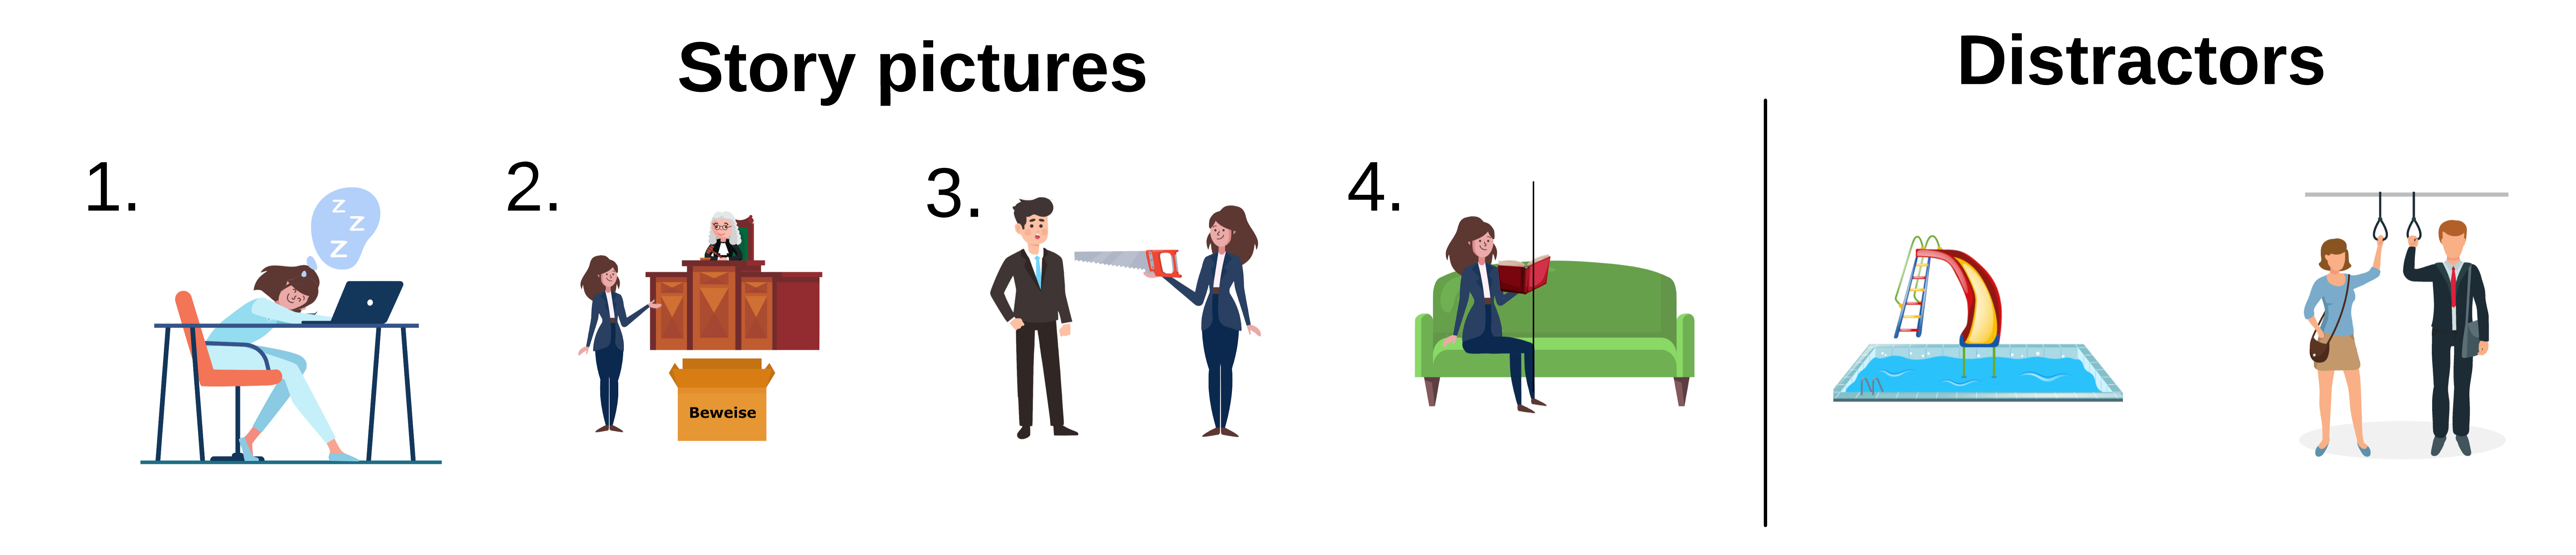
\includegraphics[scale = 0.05]{Anwalt-Saege}
	\caption{Pictures used in the card-sorting task for the [accessible, new] version of the lawyer-saw story plus two distractor pictures.}
	\label{fig:anwalt-saege-pictures}
\end{figure}

To add an interactive component to the reading task, we staged the recording session as a card-sorting game involving a confederate, whom participants believed to be another participant of the experiment. Participants first read the story aloud and after a brief delay, the confederate sorted the corresponding picture cards into the correct order. To make the card-storing task appear more difficult and thus more realistic, two distractor pictures that were unrelated to the story were presented along with the pictures corresponding to the stories (see Figure \ref{fig:anwalt-saege-pictures}). The sorting was pre-programmed and always resulted in the correct order.

While reading the stories, participants saw both the story and the corresponding pictures in the correct order. They were encouraged to first silently read and comprehend the story before reading it out loud. After reading, the participants were able to simultaneously watch the confederate sort the picture cards on their screen and provide feedback on the correctness of the order of the pictures after the task was finished. Before the actual task started, there were two example stories to practice the procedure. In cases of hesitations, repairs, exaggerated segmental articulation, or continuation rises produced by the participant in the target sentences, they were asked to repeat the reading and sorting task of the affected story at the end, with the experimenter feigning technical difficulties. A recording session lasted approximately 30 minutes.
 
Data was collected remotely via Zoom video calls in July and August 2021, with participants sitting in a quiet room at home. Participants wore headphones and were recorded on their own devices using Ennuicastr, a web application that allows for high quality multi-track recording (\url{https://ecastr.com/}). In cases where Ennuicastr did not function properly, i.e., for eight participants, we relied on backup recordings that were made in Zoom, which were, however, subject to fluctuating internet stability, which constrained the usability of some recordings (see Section \ref{section: measurements study1} for details).

We recorded 32 native speakers of German. Eight identified as male, 24 as female. Speakers were between 20 and 38 years old (mean = 26, SD = 4.2) and grew up in seven federal states of Germany but spoke no clearly discernible dialect. Two participants were raised bilingually with Russian and French as a second language, respectively, but reported German to be their dominant language. Participants reported no diagnosed speech or hearing impairments. They provided written informed consent to take part in the experiment. Participation was voluntary and there was no compensation.

\subsection{Data, annotation, and measurements} \label{section: measurements study1}

Each participant produced eight stories containing 16 target words for a total of 512 target words. We excluded six target words from Zoom recordings because they were audibly perturbed, so that 506 target words entered the analysis. Utterances were automatically segmented using WebMAUS \citep{schielAutomaticPhoneticTranscription1999, kislerMultilingualProcessingSpeech2017} and segment boundaries were manually corrected in Praat \citep{boersmaPraatDoingPhonetics2023}. Phrase boundaries and tonal events were then annotated by two trained annotators independently (one of them the author of this book) following the DIMA guidelines \citep{kuglerDeutscheIntonationModellierung2022}. In cases of disagreement, a consensus annotation was reached by consulting at least one other expert.\footnote{Inter-rater agreement before the consensus was 88\% for boundary annotation and 79\% for tonal events.} Accent status was determined with reference to position in the sentence and phrase boundary presence: Word1 was variably produced with a prenuclear or nuclear accent depending on whether it was immediately followed by a phrase boundary and Word2 was always produced with a nuclear accent. Annotations on the tonal tier were subsequently translated into GToBI pitch accent types \citep{griceGermanIntonationAutosegmentalMetrical2005}.\footnote{Inter-rater agreement for the GToBI translation was 89\%.}

In addition, we measured seven continuous prosodic parameters, namely, F0 at the Center of Mass (F0 at CoM), Delta F0, Center of Gravity (CoG), synchrony, word duration, syllable duration, and periodic energy mass. The first four parameters, all capturing different aspects of the F0 contour in the target words, as well as periodic energy mass were derived using the ProPer toolbox (\citealt{albertModelSonorityBased2023}, see also Section \ref{section: prominence form}). This toolbox allows for the quantification of prosodic information directly from the signal, without relying on turning points or other annotated landmarks. Instead, two points in time, which are derived for each syllable, are relevant for the calculation of the F0-related parameters, the Center of Mass (CoM) and the Center of Gravity (CoG, see Figure \ref{fig:proper} for a schematic depiction). The CoM is a point in time that splits the area under the periodic energy curve associated with a syllable into two equally large parts. At this time point in the stressed syllable of each target word, we measured the F0 in semitones relative to a low baseline determined individually for each speaker. This measure, F0 at CoM, thus captures the scaling of the stressed syllable. For the Delta F0 measure, we took the difference between the F0 at the CoM of the stressed syllable and of the preceding syllable in semitones, which represents a more dynamic account of F0 change towards the stressed syllable. Delta F0 can thus be regarded as a measure of tonal onglide. Furthermore, we determined the CoG in the stressed syllable as a measure of alignment by averaging time weighted by the F0 curve and multiplied by periodic energy. The CoG is reported relative to the beginning of the target word and normalized by target word duration. As a final parameter to characterize the shape of the F0 contour locally over the stressed syllable, synchrony was measured as the distance between the CoG and the CoM in milliseconds divided by syllable duration. 

To account for timing, both the duration of each target word as well as the duration of the stressed syllable within the target words (i.e., the initial syllable) were measured in milliseconds. Finally, periodic energy mass was measured as the area under the periodic energy curve associated with the stressed syllable, and represents the integral of duration and intensity in the sonorant portions of the stressed syllable. Periodic energy mass is reported as a unitless measure centered around 1. Since phrase-final words are known to undergo final lengthening \citep{wightmanSegmentalDurationsVicinity1992}, we excluded phrase-final target words (n = 157) from the statistical analysis of word duration, syllable duration, and periodic energy mass. In addition, we excluded one speaker's recordings from the periodic energy mass measures, since the audio was clipped and thus did not provide reliable intensity levels. 

\begin{figure}
		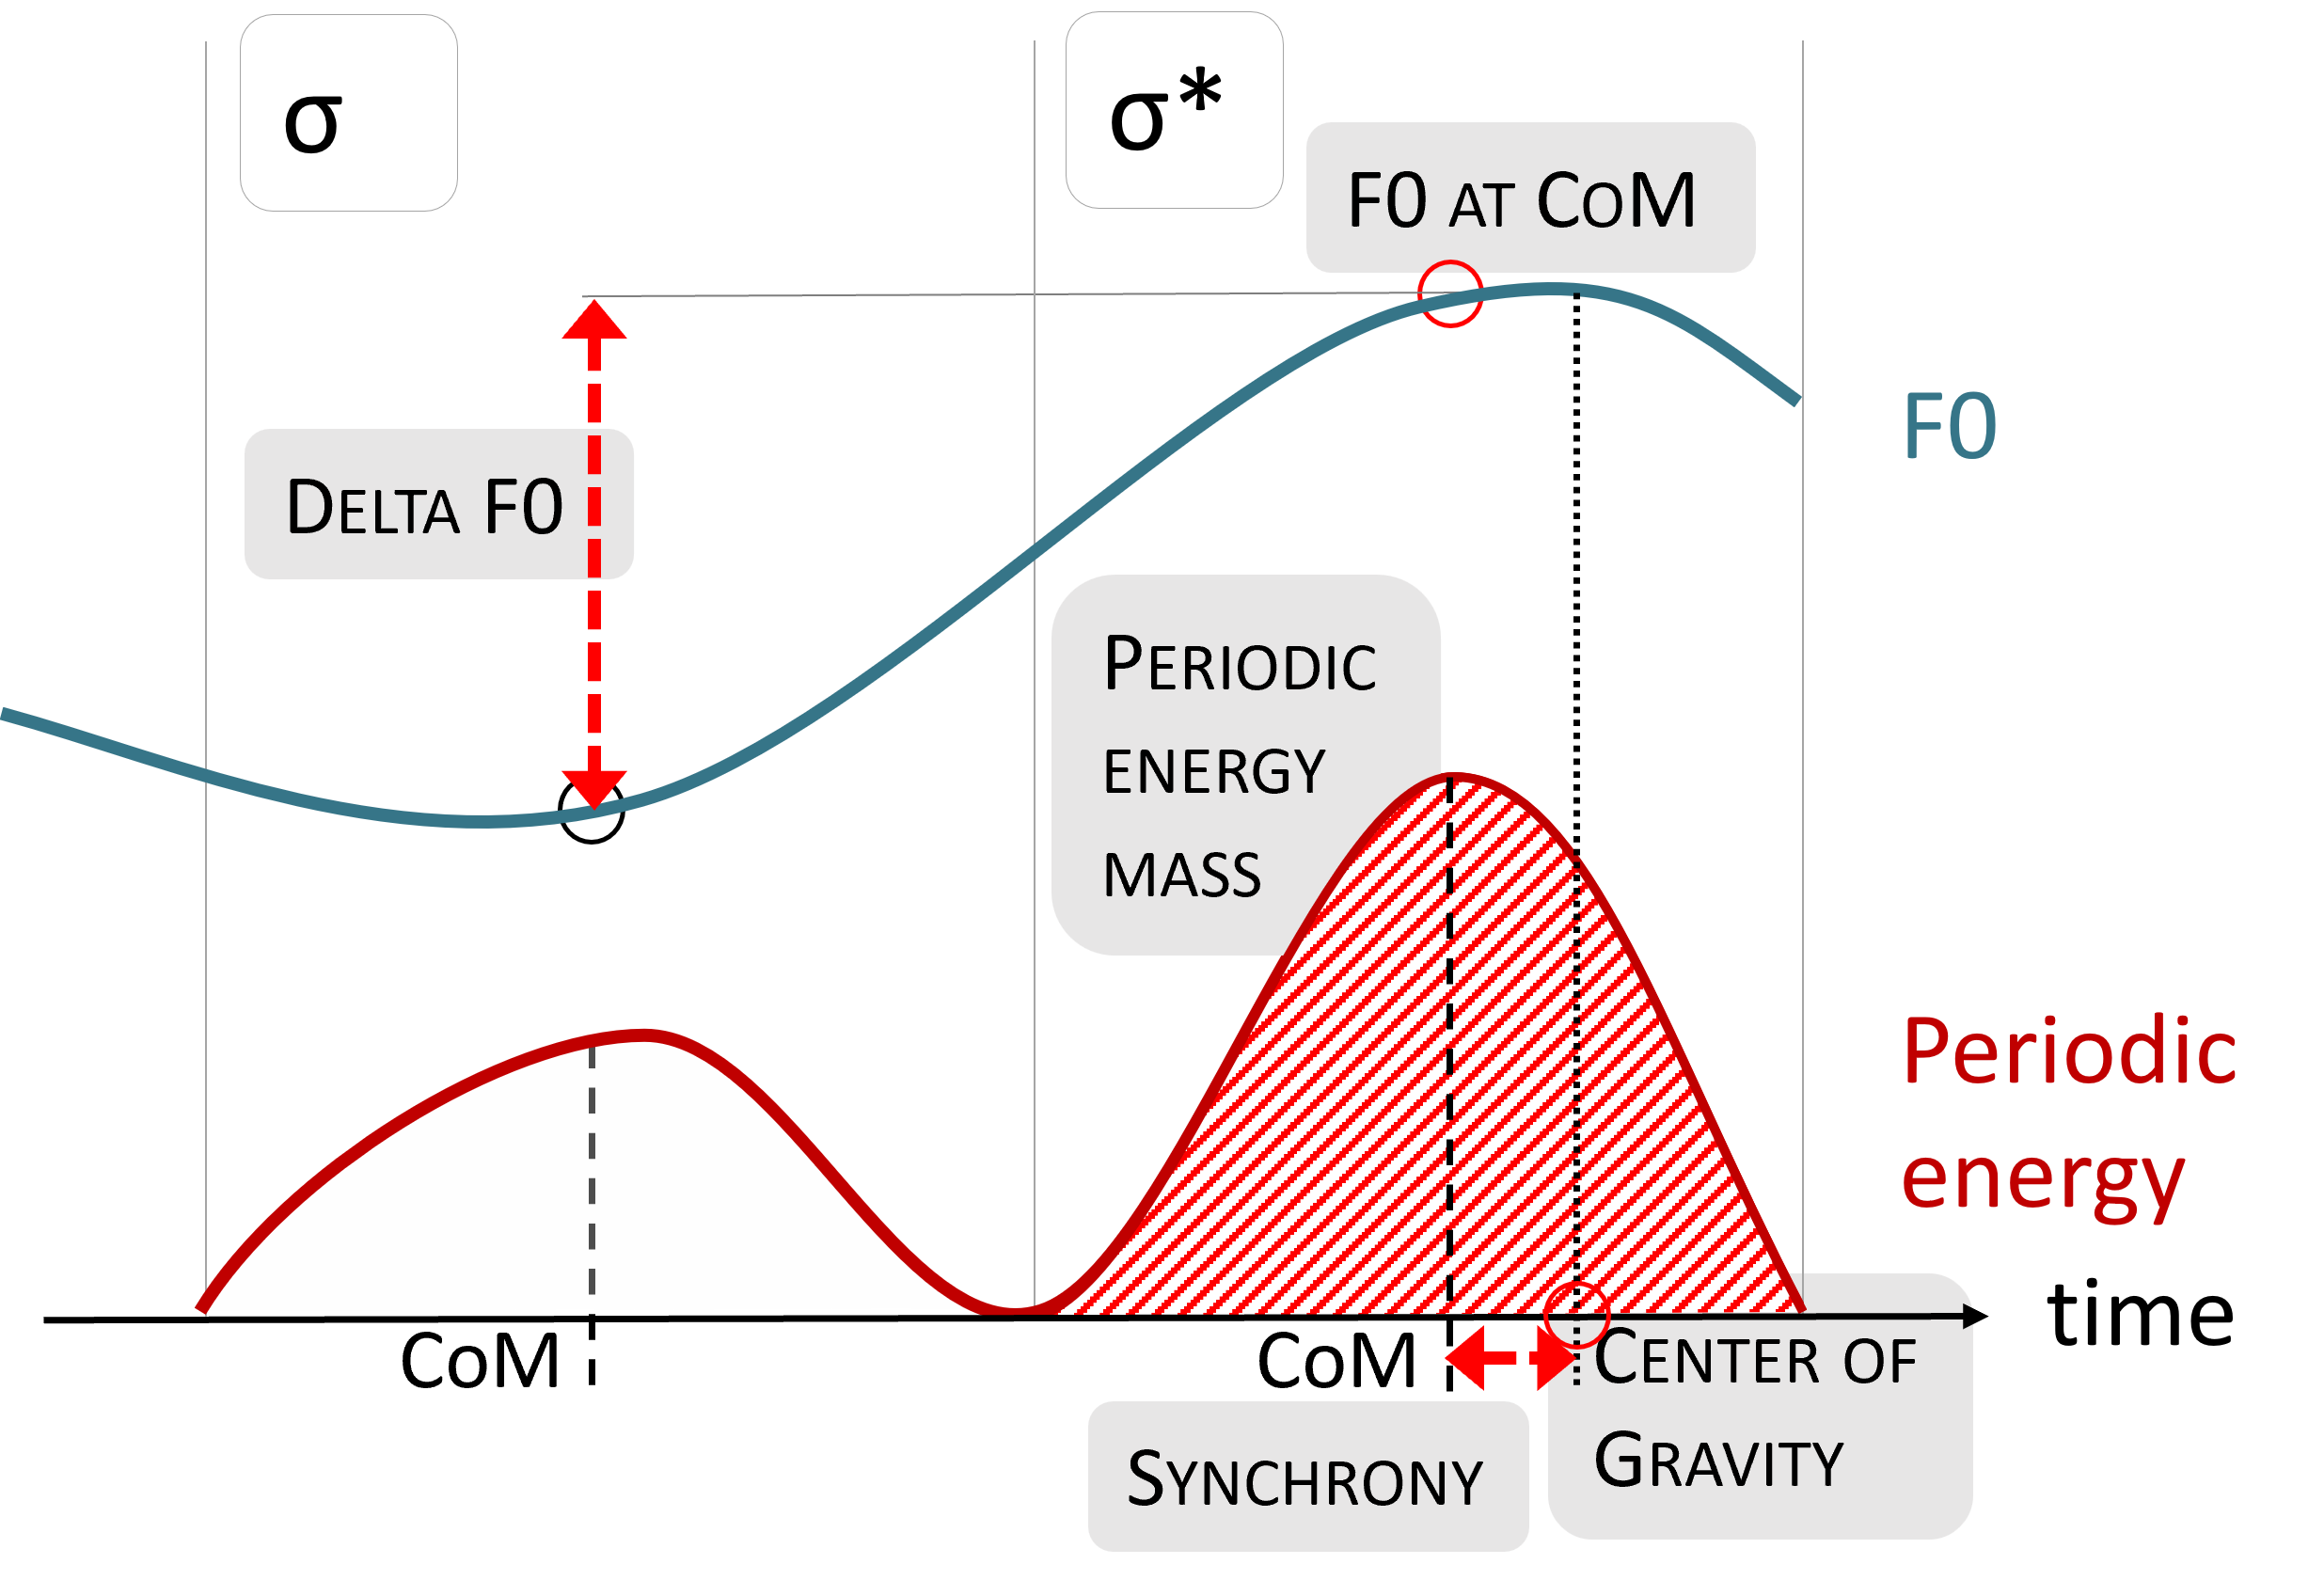
\includegraphics[scale = 0.5]{proper_schema}
	\caption{Schematic depiction of the ProPer measures, adapted from \citet{lorenzenParadigmaticSyntagmaticEffects2024}.}
	\label{fig:proper}
\end{figure}

\subsection{Statistical analysis} \label{sec: stats study1}

All analyses were conducted in R \citep{rcoreteamLanguageEnvironmentStatistical2022}, using the packages \pkg{tidyverse} \citep{wickhamWelcomeTidyverse2019}, \pkg{cowplot} \citep{wilkeCowplotStreamlinedPlot2020}, and \pkg{ggh4x} \citep{vandenbrandGgh4xHacksGgplot22024} for data wrangling and plotting, \pkg{brms} \citep{burknerBrmsPackageBayesian2017} as an interface to the Stan modeling language \citep{carpenterStanProbabilisticProgramming2017} for compiling regression models, and \pkg{cluster} \citep{maechlerClusterClusterAnalysis2022} for cluster analysis. The package \pkg{ggdendro} \citep{devriesGgdendroCreateDendrograms2024} was used to create a dendrogram. All data and scripts used to perform the analyses presented here are available from the accompanying OSF repository (\url{https://osf.io/m5xwe/}). 

We compiled separate Bayesian mixed-effects regression models for accent status, accent type, and each of the seven prosodic parameters. For the categorical parameters, we ran a binary logistic regression model using accent status as the dependent variable (levels: \textit{prenuclear}, \textit{nuclear}) and a cumulative regression model with accent type as the dependent variable. Here, we treated pitch accent type as an ordered factor according to the ranking established by \citet{baumannPerceptualProminencePitch2015}, namely, from most to least prominent: L+H* > L*+H > H* > H+!H* > H+L* > !H* > L*. The models for the continuous parameters contained the z-scored parameter as the dependent variable. Z-scoring was done to ensure the comparability of the different parameters despite the different units in which they were measured. Each model included information status (levels: \textit{new}, \textit{accessible}) and position (levels: \textit{Word1}, \textit{Word2}) as well as their interaction as predictors, random intercepts for speaker and word, and random slopes for the by-speaker effects of information status and position.\footnote{Note that the accent status model was run only on the subset of the data including Word1 and thus did not include position as a predictor since Word2 was always produced with a nuclear accent.} The random slopes capture the fact that speakers may differ in whether and to what degree they modulate certain parameters in order to encode information status, which makes them crucial to accounting for and analyzing inter-speaker variability.

Four sampling chains ran for 14,500 iterations with 12,000 warm-up iterations for a total of 10,000 posterior draws. We set weakly informative, normally distributed priors centered around zero with a standard deviation of one for the regression coefficients and used default priors provided by \pkg{brms} for the remaining model parameters. Model fits were assessed visually by inspecting the posterior predictive checks and by ensuring that the models yielded no Rhat values larger than one.

For each model, we report the regression coefficient $\beta$ and 90\% credible intervals (CrIs) under the posterior distributions as well as the posterior probability that $\beta$ is larger than zero: Pr($\beta$\textgreater{}0). While the interpretation of a Bayesian regression model allows for a gradient evaluation of the effects under investigation, it is useful to specify reliability criteria that allow for a binary decision, which facilitates comparisons to analyses conducted in the frequentist framework. We thus consider the effect of a contrast specified by the predictor variables ``reliable" if the 90\% credible interval (CrI) does not include 0 and the probability that $\beta$ is larger than zero is higher than 0.95 or lower than 0.05. 

For a systematic approach to investigating individual speaker strategies, we extracted the random slope estimates from the models with the continuous dependent variables and ran a hierarchical agglomerative cluster analysis on those estimates.\footnote{Note that we conduct this analysis only on the continuous variables, which were modeled via linear regression. The categorical variables were modeled via logistic and cumulative regression, so that the model estimates are on a different scale, namely log odds. Running the same cluster analysis on these differently scaled numbers would confound the results.} This analysis is modeled after \citet{baumannWhatMakesWord2018}, who conducted a similar analysis on the random slopes of their frequentist models. First, a distance matrix was computed, estimating the Euclidean distances between the random slope estimates. Second, a hierarchical cluster analysis was performed on this distance matrix using the Ward D.2 algorithm. The clustering algorithm operates bottom-up, i.e., initially, every speaker represents their own cluster and then the speakers with the smallest distances are grouped together iteratively until all speakers are merged together in one cluster. In order to determine the optimal number of clusters, we rely on the average silhouette width. Silhouette width is a measure of well-formedness of clusters, quantifying how similar members of the same cluster are to each other and how dissimilar members of different clusters are. Silhouette width values range from 0 to 1 with 0 indicating that there is no cluster structure in the data and 1 meaning that all data cluster perfectly into separate groups \citep{levshinaHowLinguisticsData2015}. A silhouette width above 0.25 can be interpreted as reasonable evidence for a cluster structure being present in the data \citep[88]{kaufmanFindingGroupsData1990}. 

\section{Results} \label{sec:Production 1 results}

\subsection{Overall results} \label{sec:Production 1 overall results}

This section considers the overall results averaged across all speakers to establish a baseline, which allows for comparisons regarding how and to what extent individuals differ from this group average. Figure \ref{fig:example_pitchtracks} shows two exemplary productions of the two target noun phrases in two different utterances produced by two different speakers to illustrate the general structure of the data.\footnote{These figures were created using the R package \pkg{praatpicture} \citep{puggaard-rodePraatpicturePraatPicture2024}.} In the utterance visualized in the top panel, the target words were produced with a typical hat pattern, a rising accent on Word1 and a falling accent on Word2, which is very frequent in our data. The utterance in the bottom panel represents a common alternative production with two subsequent rising accents on the target words. Target words were always produced with a pitch accent (prenuclear or nuclear), which was annotated on the Accent type tier. Due to the nature of the target sentences, phrase boundaries were very frequently produced after the first target word (in 58\% of cases), as, for example, in the top panel of Figure \ref{fig:example_pitchtracks} but rarely after Word2 (only 4\%).

\begin{figure}

%     \subfloat{
    {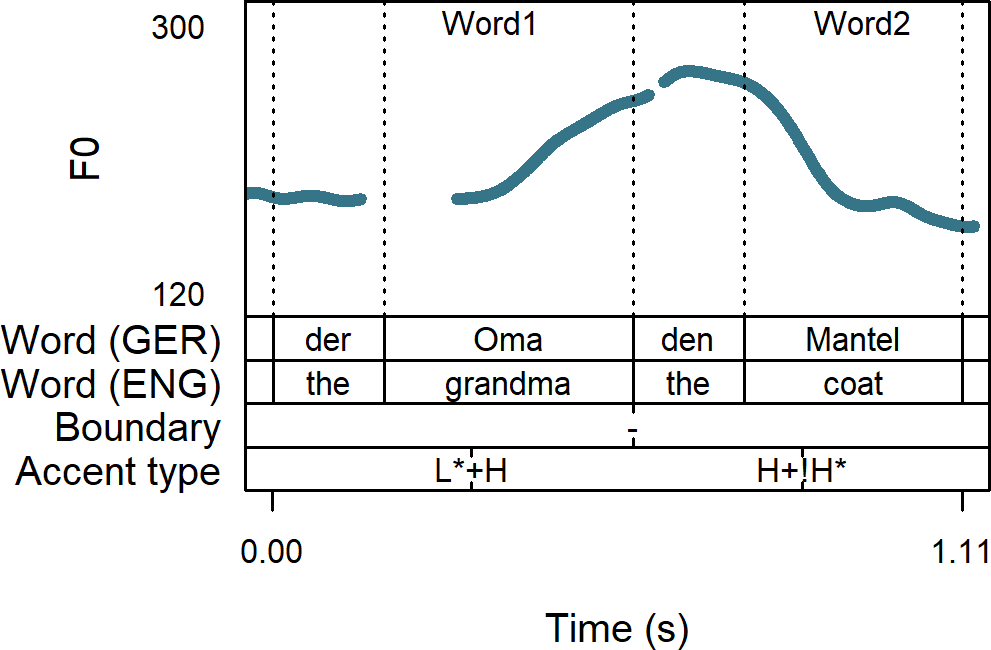
\includegraphics[width=.7\textwidth]{pitchtrack_s12oma_cropped.png} }
%     }

    \bigskip

%     \qquad
%     \subfloat{
    {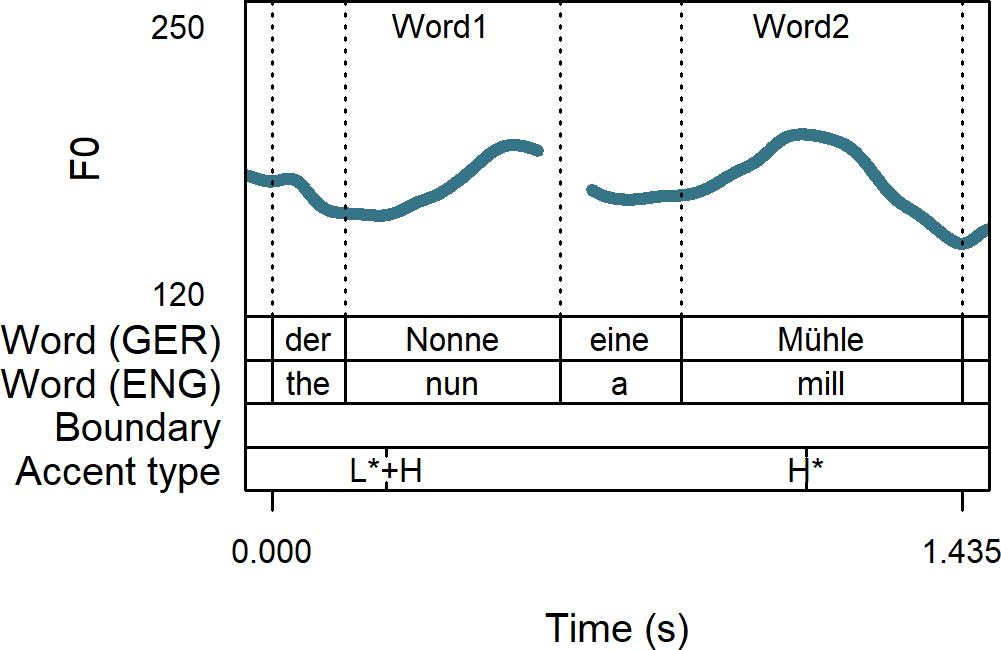
\includegraphics[width=.7\textwidth]{pitchtrack_s10nonne_cropped.png} }
%     }
    \caption{Examples of the F0 contour realized over the target words in two typical productions with DIMA boundary annotation and GToBI accent type.}
    \label{fig:example_pitchtracks}
\end{figure}

Since Word1 and Word2 were often produced differently, e.g., Word1 was always produced with a rising intonation, while Word2 often exhibits falling F0, we will consider the effects of information status on Word1 and Word2 separately for each prosodic parameter. In terms of metrical structure, Word2 was always produced with a nuclear accent, while Word1 either received a prenuclear or a nuclear accent depending on whether it was followed by a phrase boundary. Figure \ref{fig:s1_accent_statustype} (left) illustrates the distribution of accent status by word position and information status. It is evident that accent status in Word1 is probabilistically modulated by information status: New target words are more likely to be produced with a nuclear accent than accessible target words, i.e., the former tend to occupy metrically stronger, more prominent positions than the latter. According to the Bayesian regression model (see Table \ref{table:model_prosodic-discrete}), this effect is fairly strong, albeit not quite reliable following the criteria specified in Section \ref{sec: stats study1}.

\begin{figure}
		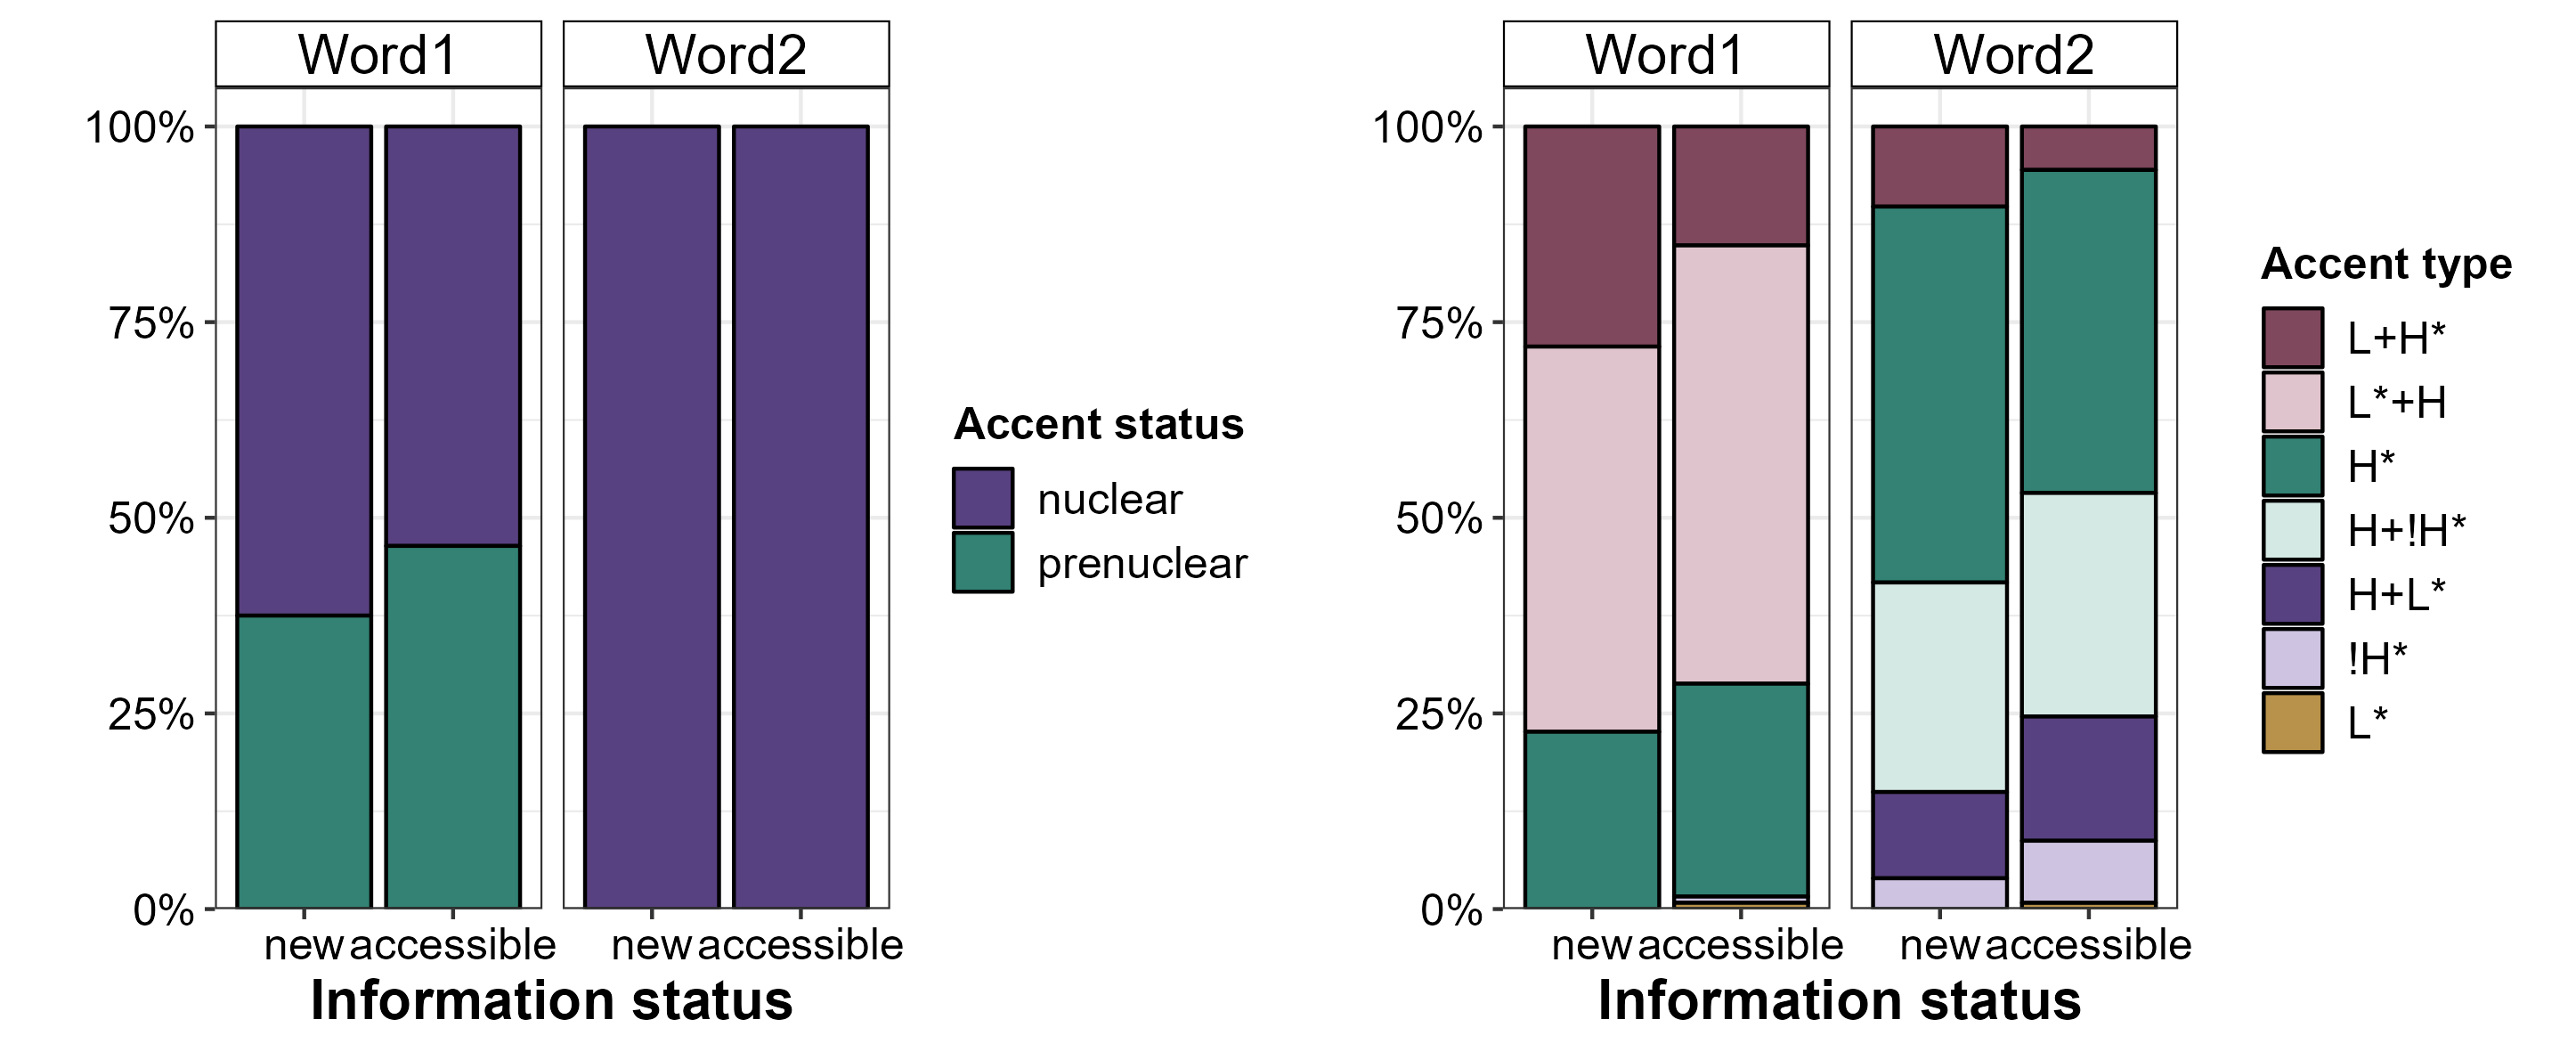
\includegraphics[scale = 0.5]{s1_accent_statustype}
	\caption{Barplots of the distributions of accent status and accent type by position and information status.}
	\label{fig:s1_accent_statustype}
\end{figure}

\begin{table}[]
\begin{tabular}{lrrr}
\lsptoprule
Variable    & $\beta$ & 90\% CrI  & Pr($\beta$\textgreater{}0) \\ \hline
Accent status (Word1)    & 0.12       & {[}0.00; 0.24{]}  & 0.95                          \\
Accent type (Word1)    & 0.61       & {[}0.21; 1.02{]}  & 0.99                          \\
Accent type (Word2)         & 0.66       & {[}0.23; 1.09{]} & 0.99                          \\
\lspbottomrule
\end{tabular}
\caption{Model parameters describing the effects of information status in the categorical prosodic parameters.}
\label{table:model_prosodic-discrete}
\end{table}

As for accent type, Figure \ref{fig:s1_accent_statustype} (right) illustrates the different accent type distributions produced on Word1 and Word2. Word1 was often produced with the high rising accents L*+H and L+H*, while falling accents, such as H+!H* and H+L*, occur only in Word2. Within each position, information status further modulates the likelihood of certain accent types occurring. Accent types in Figure \ref{fig:s1_accent_statustype} are ordered according to their inherent prominence following \citet{baumannPerceptualProminencePitch2015}. In both Word1 and Word2, new target words are produced with higher proportions of more prominent accent types, e.g., L+H* accents are more likely to be produced on new than on accessible target words, while accessible target words are more often produced with less prominent accent types, e.g., H* in Word 1 or H+L* and !H* in Word2. These differences are statistically reliable in both positions (see Table \ref{table:model_prosodic-discrete}).

Turning to the continuous phonetic parameters, Table \ref{table:model_parameters_Word1} summarizes the key model estimates for all continuous parameters for Word1. Generally, we expect higher values (associated with higher prominence) in new as compared to accessible referents for all continuous parameters (see also Section \ref{section: prominence form}), which is the case when the posterior estimate $\beta$ takes a positive value. In case of a negative $\beta$ estimate, the prosodic parameter in question takes on average higher values in accessible than in new referents. According to the reliability criteria specified in the previous section, Delta F0 is the only reliable cue to information status in Word1. More specifically, new referents are consistently produced with a higher Delta F0 than accessible referents. Higher F0 at CoM and longer word duration also appear to be relatively strong cues to newness. While synchrony displays a somewhat weaker tendency for higher values in the new referents, CoG and syllable duration do not appear to encode the information status contrast systematically. Finally, periodic energy mass exhibits an unexpected albeit weak tendency for higher values in accessible referents.

\begin{table}[]
\begin{tabular}{lrrr}
\lsptoprule
\multicolumn{4}{c}{Word1} \\ \hline
Variable    & $\beta$ & 90\% CrI  & Pr($\beta$\textgreater{}0) \\ \hline
F0 at CoM    & 0.12       & {[}0.00; 0.24{]}  & 0.95                          \\
Delta F0    & 0.30       & {[}0.15; 0.44{]}  & 1.00                          \\
Center of Gravity            & 0.03       & {[}-0.11; 0.16{]}  & 0.63                          \\
Synchrony            & 0.09       & {[}-0.04; 0.22{]}  & 0.88                          \\
Word duration            & 0.15       & {[}-0.01; 0.31{]}  & 0.94                          \\
Syllable duration & 0.05       & {[}-0.15; 0.24{]}  & 0.66                             \\
Periodic energy mass         & -0.10       & {[}-0.34; 0.14{]} & 0.25                          \\
\lspbottomrule
\end{tabular}
\caption{Model parameters describing the effects of information status in Word1.}
\label{table:model_parameters_Word1}
\end{table}

Regarding Word2 (see Table \ref{table:model_parameters_Word2}), again, Delta F0 emerges as the only reliable cue to information status, with new referents being produced with on average higher Delta F0 than accessible referents. There is also evidence that higher synchrony values are found in new referents. Unexpectedly, it appears that F0 at CoM is on average \textit{lower} in new than in accessible referents. A weaker tendency to be found is that word duration is longer in new than in accessible referents. CoG, syllable duration, and periodic energy mass again seem to play only a minor role in information status marking, similar to the findings for Word1.

\begin{table}[]
\begin{tabular}{lrrr}
\lsptoprule
\multicolumn{4}{c}{Word2} \\ \hline
Variable    & $\beta$ & 90\% CrI  & Pr($\beta$\textgreater{}0) \\ \hline
F0 at CoM    & -0.08       & {[}-0.20; 0.05{]}  & 0.15                          \\
Delta F0    & 0.43       & {[}0.29; 0.58{]}  & 1.00                          \\
Center of Gravity            & -0.06       & {[}-0.20; 0.08{]}  & 0.23                          \\
Synchrony            & 0.12       & {[}-0.01; 0.24{]}  & 0.93                          \\
Word duration            & 0.06       & {[}-0.04; 0.17{]}  & 0.85                          \\
Syllable duration & 0.05       & {[}-0.09; 0.17{]}  & 0.73                             \\
Periodic energy mass         & -0.03       & {[}-0.19; 0.14{]} & 0.40                          \\
\lspbottomrule
\end{tabular}
\caption{Model parameters describing the effects of information status in Word2.}
\label{table:model_parameters_Word2}
\end{table}

\subsection{Individual strategies}

After reporting on the averaged results across all speakers, this section explores how individual speakers might differ from or mirror this group behavior. As described in the previous section, both accent status (in Word1) and accent type are relatively strong cues to information status. However, this does not necessarily mean that all speakers make use of these phonological categories to encode information status or that they make use of them to the same extent. Figure \ref{fig:s1_accentstatus_byspeaker} displays the accent status distributions (only for Word1) for all speakers, showing considerable inter-individual variability. Four speakers, in fact, produce only nuclear accents (i.e., always produce a phrase boundary after Word1, third row in Figure \ref{fig:s1_accentstatus_byspeaker}) and one speaker (s24, fourth row) always realizes Word1 with a prenuclear accent. None of the speakers show a perfect one-to-one correspondence between nuclear accents on new referents on the one hand and prenuclear accents on accessible referents on the other, although speakers s2 and s18 (first row) come very close. Almost half of the speakers (n = 15) produce more nuclear accents in new referents, seven speakers make no difference between new and accessible and the remaining ten speakers show the reverse pattern, with more nuclear accents on accessible referents than on new ones.

\begin{figure}
		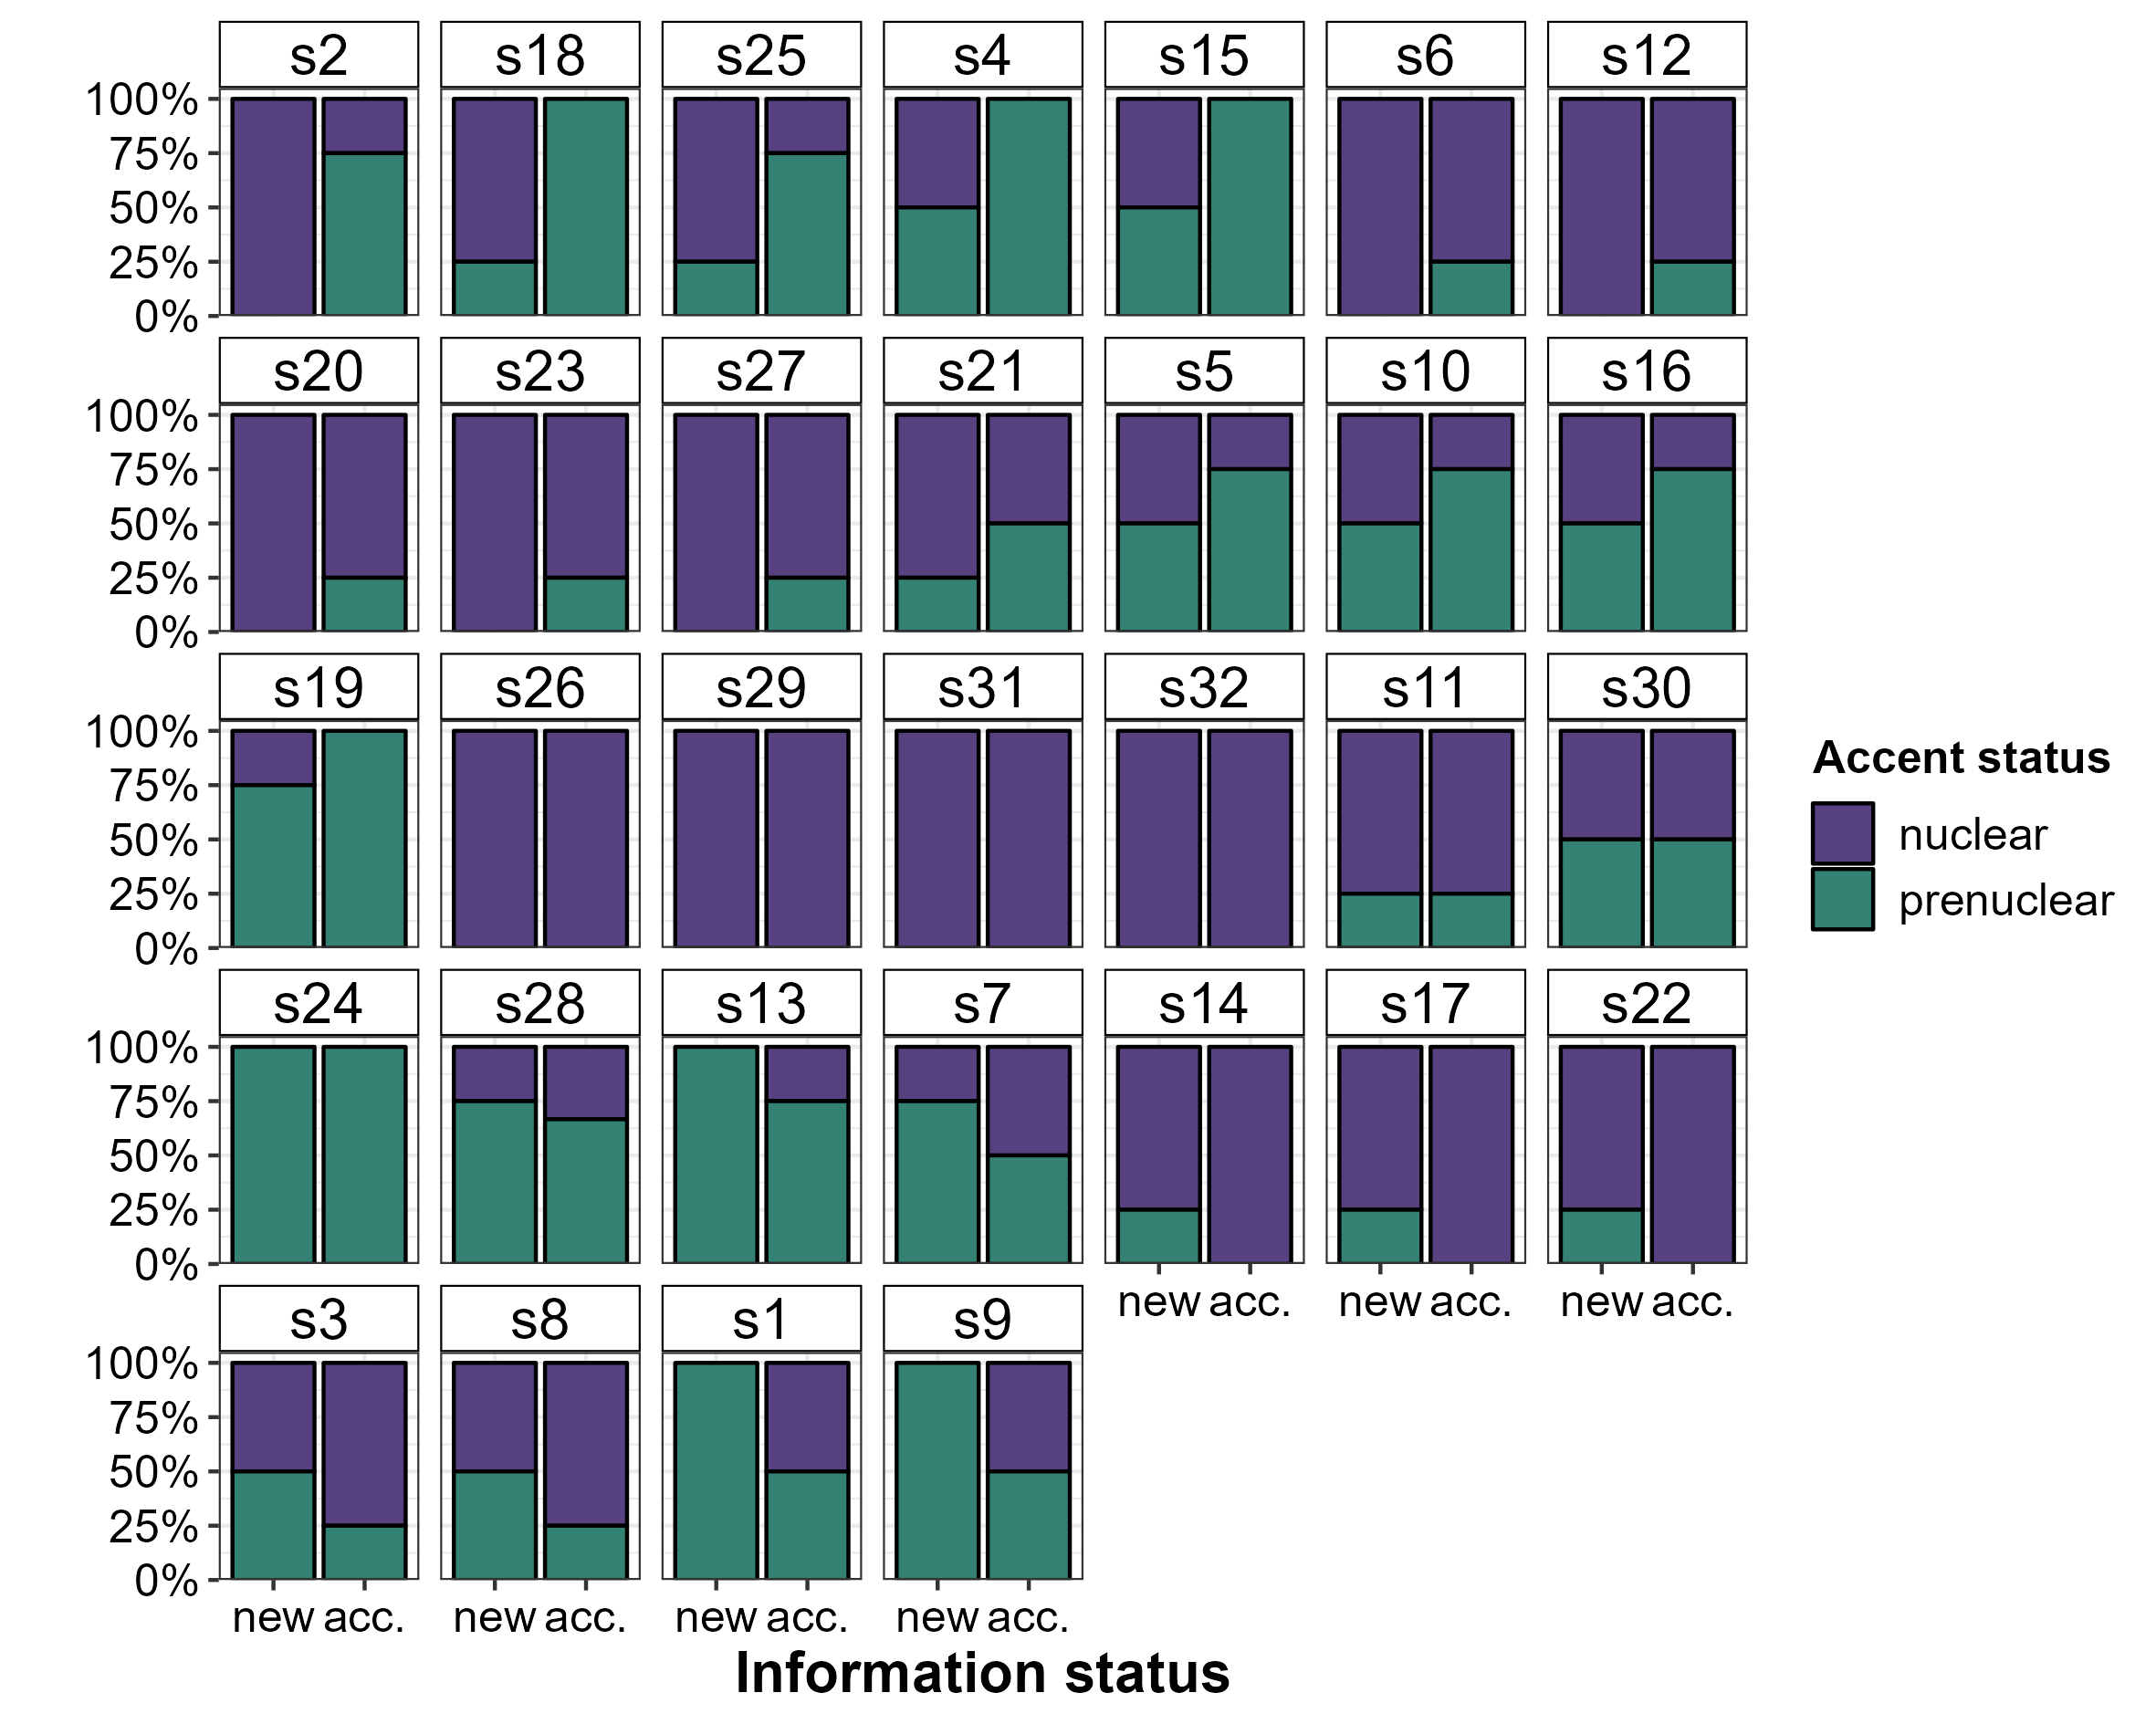
\includegraphics[scale = 0.6]{s1_accent_status_byspeaker}
	\caption{Barplots of accent status distributions on Word1 by information status per speaker.}
	\label{fig:s1_accentstatus_byspeaker}
\end{figure}

A comparable degree of variability emerges for pitch accent types. In Figure \ref{fig:s1_accenttype_byspeaker}, we consider eight exemplary speakers for reasons of space and ease of comprehensibility (plots for all speakers can be found in Appendix \ref{Appendix A}). Speakers vary in how many different accent types they produce, e.g., speaker s31 (top row, left) produces only two different accent types in both positions, while other speakers produce up to five different accent types across both positions. Generally, speakers are relatively consistent within their own productions, most using only one or two different accent types per position and information status condition. Crucially, there are differences in the use of accent type as a cue to information status. In Figure \ref{fig:s1_accenttype_byspeaker}, the two speakers in the top row show a tendency to produce new target words with more prominent accent types than accessible ones in both Word1 and Word2. This is in fact the pattern exhibited by the largest group of speakers (34\%). Interestingly, these two speakers (s31 and s26) both produce only nuclear accents on Word1 (see Figure \ref{fig:s1_accentstatus_byspeaker}), so that they potentially compensate for the absence of accent status as a cue to information status by producing accent type differences instead. The two speakers in the second row of Figure \ref{fig:s1_accenttype_byspeaker} produce more prominent accent types on new target words only in Word1, while there is no difference between new and accessible in Word2, which is a pattern repeated by 16\% of speakers in our data. The reverse strategy is embodied by the speakers in the third row (and in 28\% of our speakers), who produce more prominent accent types for new referents only in Word2. Finally, there are also speakers (22\% in our data), such as those in the bottom row of Figure \ref{fig:s1_accenttype_byspeaker}, who produce more prominent accent types on accessible target words as compared to new ones. Here, speaker s32 also produces only nuclear accents on Word1, so that neither categorical prosodic parameter serves as a cue to information status for this speaker. However, speakers failing to make categorical distinctions between new and accessible target words could still make use of more subtle phonetic cues to encode information status. 

\begin{figure}
		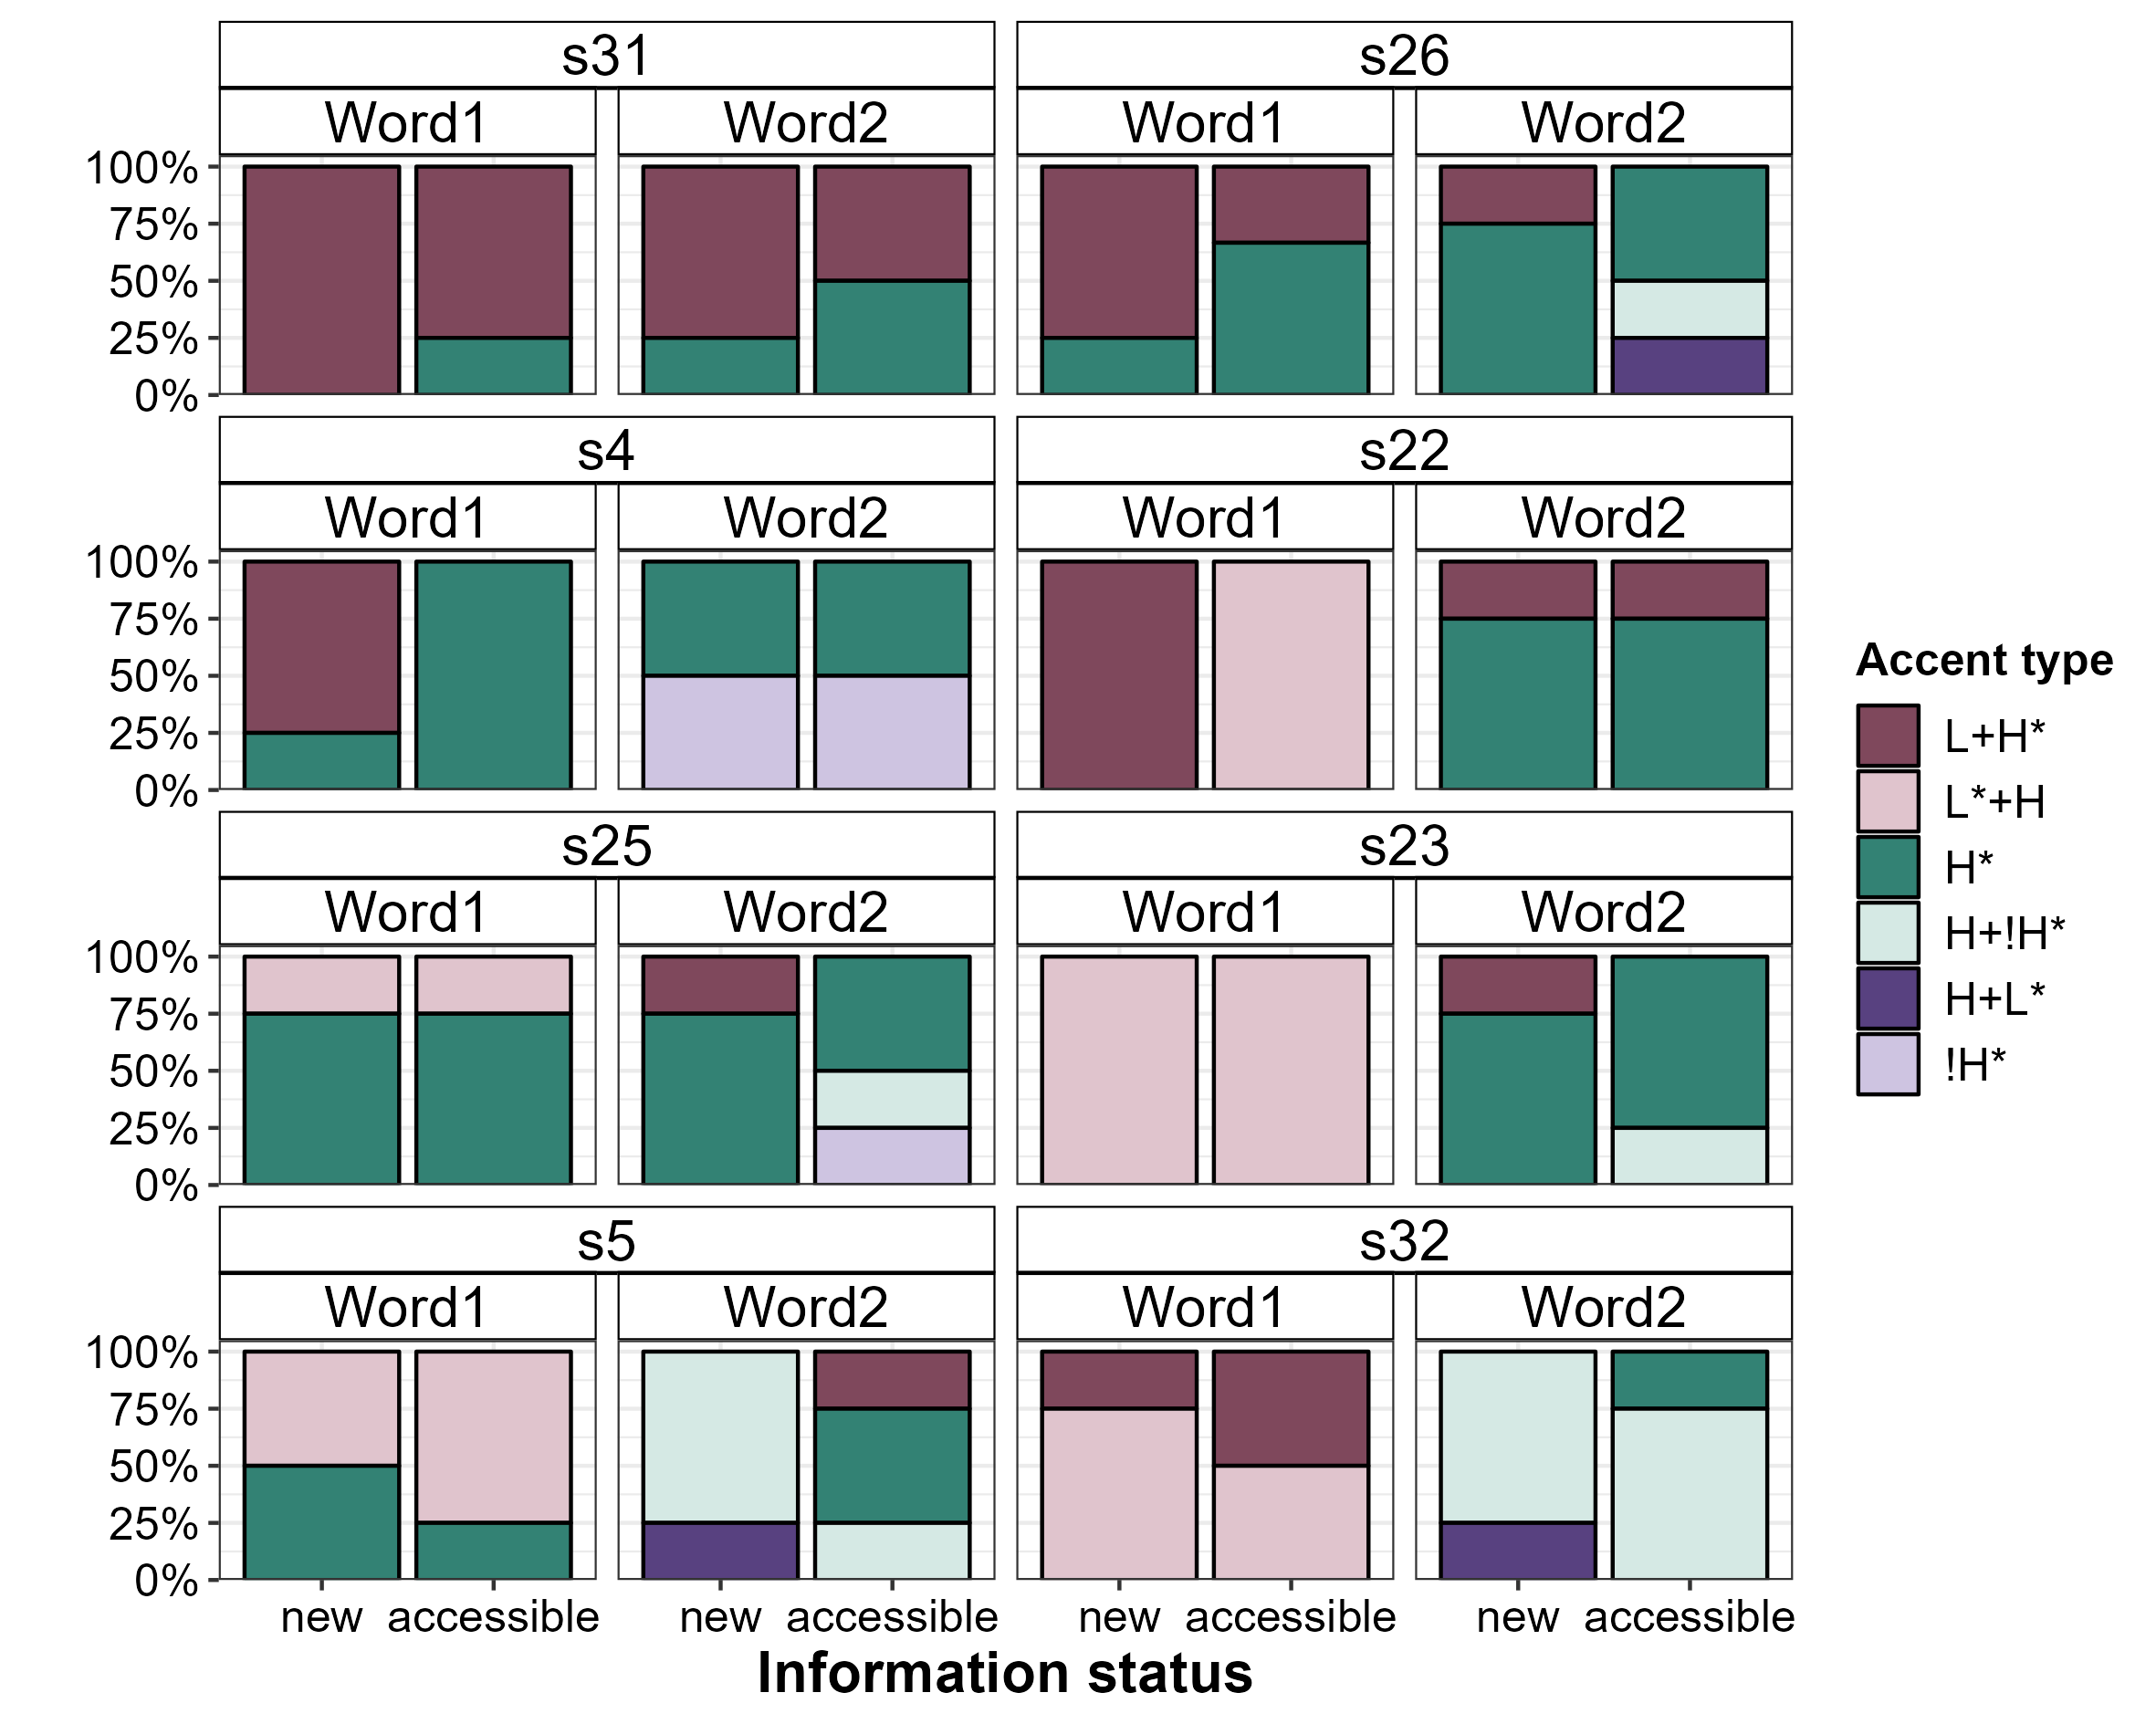
\includegraphics[scale = 0.6]{s1_accent_type_byspeaker}
	\caption{Barplots of accent type distributions by position and information status for eight exemplary speakers.}
	\label{fig:s1_accenttype_byspeaker}
\end{figure}

In Section \ref{sec:Production 1 overall results}, Delta F0 was the most reliable continuous prosodic cue to information status, with higher Delta F0 indicating newness and lower Delta F0 accessibility. However, this does not necessarily mean that every single speaker uses Delta F0 in this way. Word duration constitutes another relatively strong and consistent cue to information status across both word positions, which is nevertheless slightly less reliable than Delta F0. To illustrate how diverse speaker behavior can be beyond group averages, Figure \ref{fig:speaker_examples} depicts the distributions of z-scored Delta F0 and word duration values separated by information status for four exemplary speakers. Speaker s22 (Figure \ref{fig:speaker_examples}, top row) produces on average higher Delta F0 in new target words, however, the distributions of word duration for new and accessible target words are highly overlapping and the difference between the means is very small, indicating that this speaker makes use of Delta F0 but not duration to encode information status. For speaker s10 (Figure \ref{fig:speaker_examples}, second row), although there is quite a bit of overlap for the distributions of Delta F0 and word duration, both exhibit on average higher values in the new condition, so that both serve as a cue to newness for this speaker. By contrast, speaker s1 (Figure \ref{fig:speaker_examples}, third row) seems to use longer word duration for new as compared to accessible target words, but (if anything) slightly lower Delta F0. Finally, speaker s14 (Figure \ref{fig:speaker_examples}, bottom row) displays neither an effect of information status on Delta F0 nor on word duration, with both cue distributions largely overlapping. To summarize, by looking at four different speakers' use of two parameters, we find four different strategies, indicating that there may be as many different individual strategies as cue combinations.

\begin{figure}
		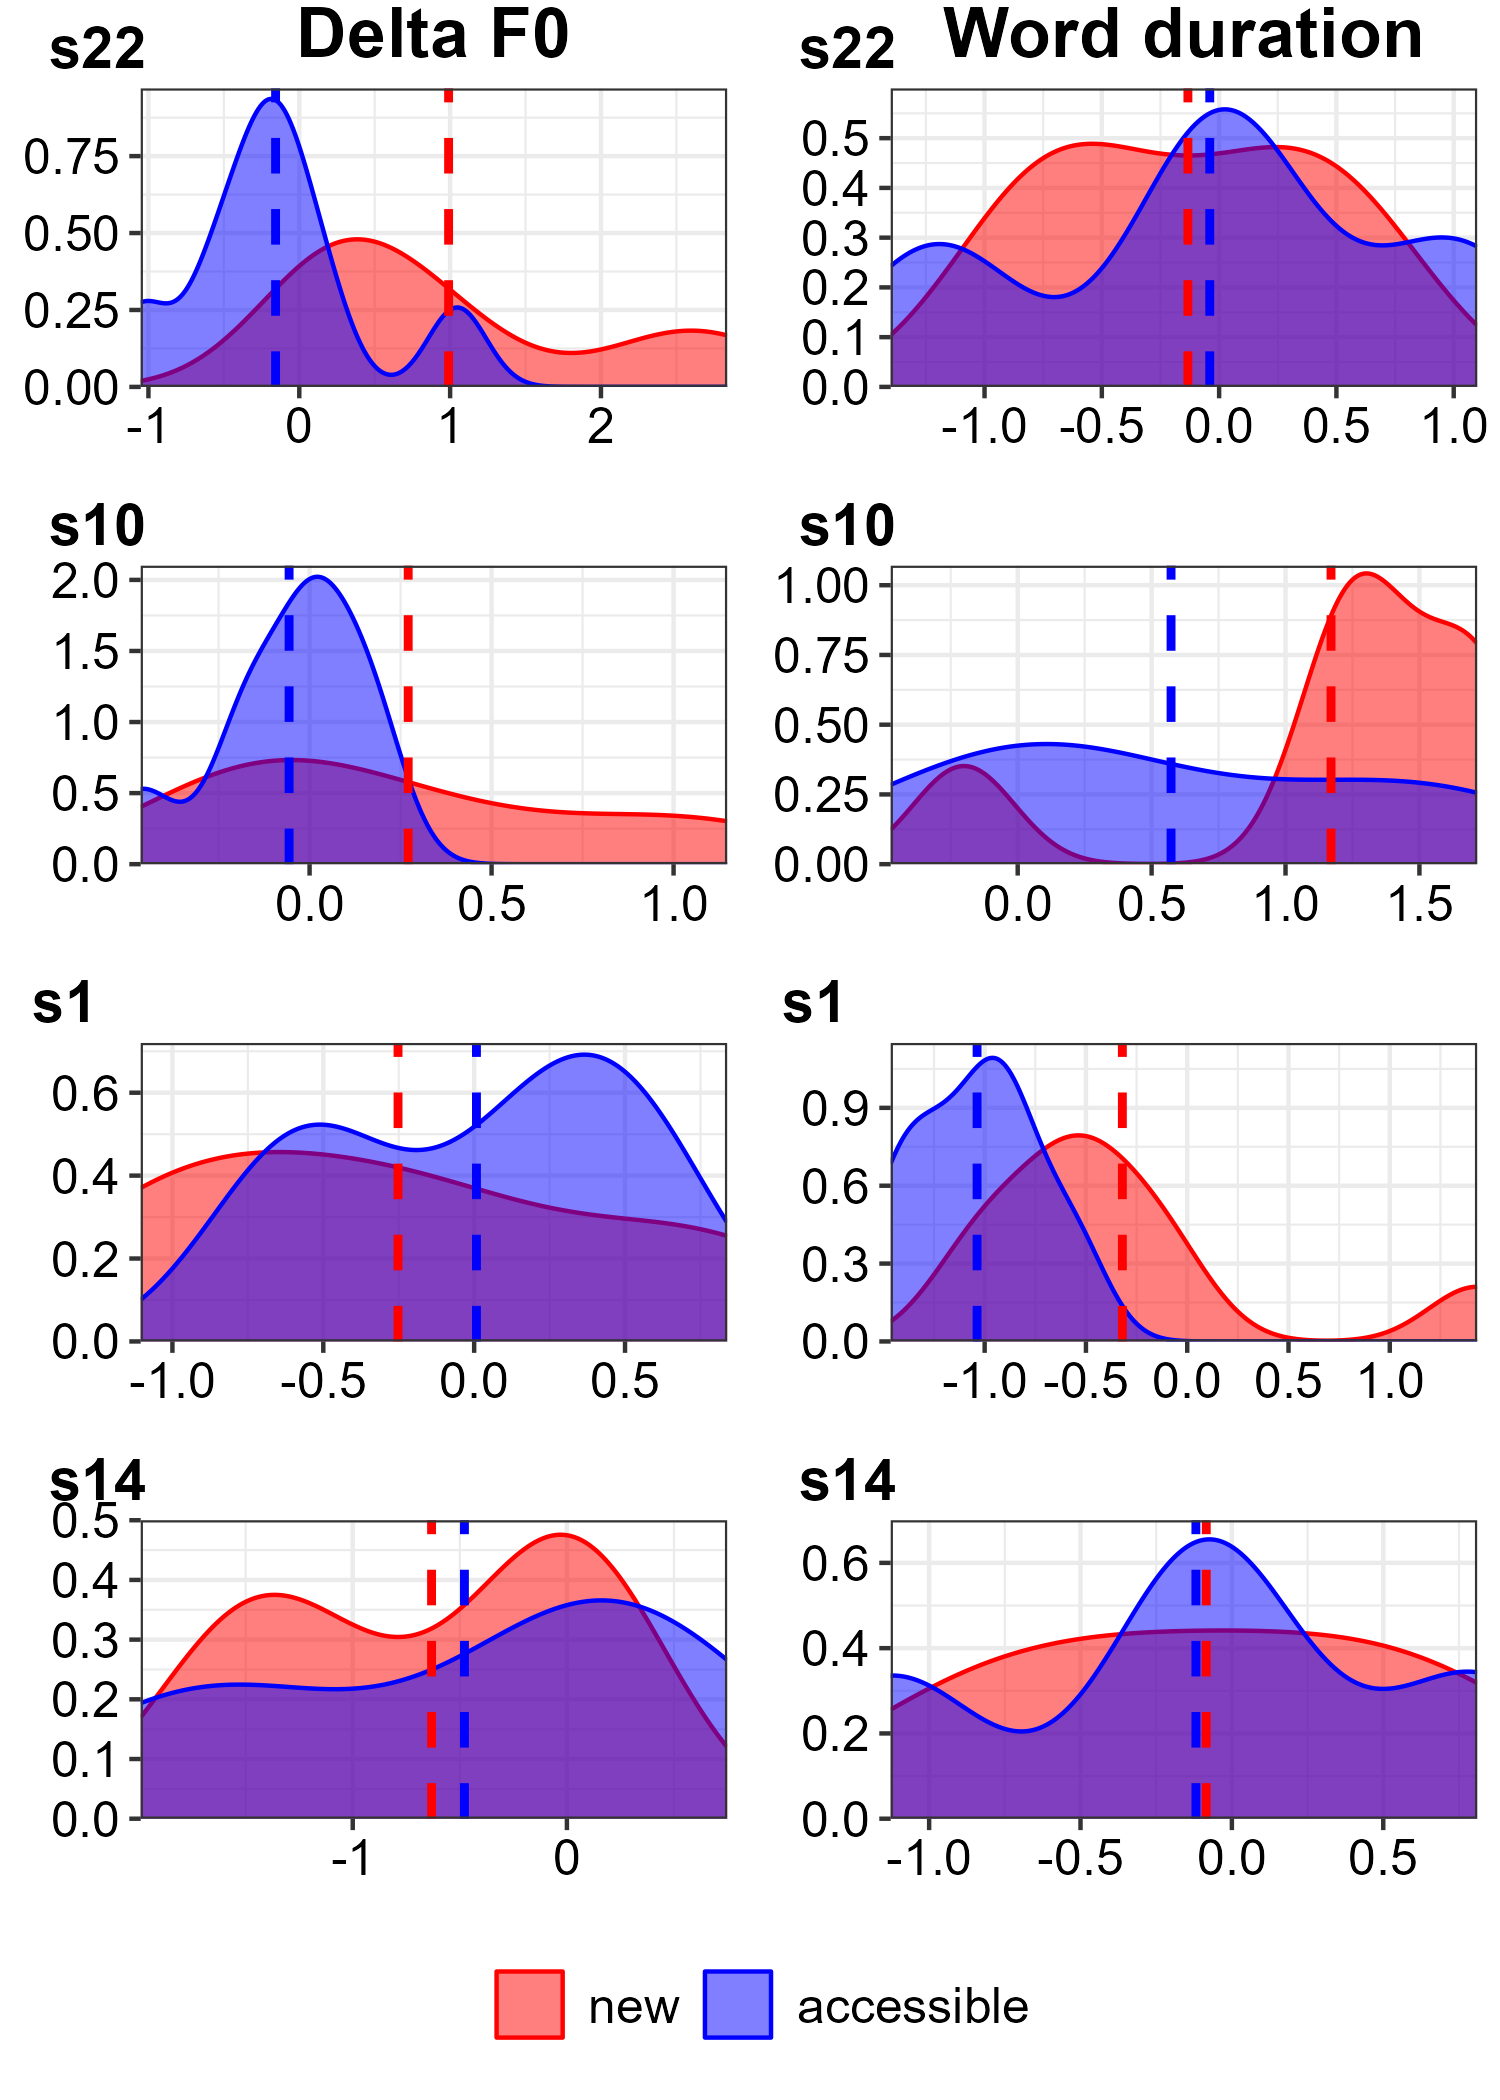
\includegraphics[scale = 0.6]{speaker_examples}
	\caption{Plots showing distributions and means (dashed lines) of z-scored Delta F0 (left panels) and word duration (right panels) by information status for four exemplary speakers.}
	\label{fig:speaker_examples}
\end{figure}

For a more complete picture of individual speakers' usage of all seven prosodic parameters investigated here, Table \ref{table:zscore_diffs} summarizes the differences between new and accessible target words in the z-scored parameters per speaker. Here, darker shading indicates larger positive differences, i.e., the parameters serve as stronger cues to information status in the expected direction with higher values for new than for accessible target words. Focusing first on the columns, it is apparent that higher Delta F0 is used by most speakers to mark newness (25 out of 32), which reflects the result of Delta F0 being the strongest cue to information status overall. Nevertheless, some speakers do not seem to make use of Delta F0 in this way, instead relying on other parameters. For example, speaker s1 marks newness only by longer word and syllable duration, whereas all other parameters are unexpectedly higher in accessible than in new words. Speaker s5 does not appear to modulate any of the parameters in the expected direction, which is evident from the mostly negative differences in the respective row. In contrast, speaker s19 encodes information status maximally redundantly, making use of all seven continuous prosodic parameters. These latter two speakers represent the most extreme cases of information status marking, with a variety of different strategies existing on the continuum between these two points.

\begin{table}[]
\begin{tabular}{llllllll}
\lsptoprule
             & \begin{tabular}[c]{@{}l@{}}F0 at \\ CoM\end{tabular} & \begin{tabular}[c]{@{}l@{}}Delta \\ F0\end{tabular} & \begin{tabular}[c]{@{}l@{}}Center\\ of \\ Gravity\end{tabular} & Synchrony           & \begin{tabular}[c]{@{}l@{}}Word\\ duration\end{tabular} & \begin{tabular}[c]{@{}l@{}}Syllable\\ duration\end{tabular} & \begin{tabular}[c]{@{}l@{}}Periodic \\ energy\\ mass\end{tabular} \\ \hline
s1  & -0.29                                                         & -0.26                                                        & -0.47                                                                   & -0.21                        & \cellcolor[HTML]{9B9B9B}0.72                                     & \cellcolor[HTML]{9B9B9B}0.68                                         & -0.08                                                                      \\
s2  & -0.17                                                         & \cellcolor[HTML]{C0C0C0}0.42                                 & \cellcolor[HTML]{C0C0C0}0.17                                            & \cellcolor[HTML]{C0C0C0}0.43 & \cellcolor[HTML]{EFEFEF}0.08                                     & \cellcolor[HTML]{C0C0C0}0.34                                         & \cellcolor[HTML]{9B9B9B}0.97                                               \\
s3  & \cellcolor[HTML]{C0C0C0}0.49                                  & \cellcolor[HTML]{C0C0C0}0.27                                 & \cellcolor[HTML]{C0C0C0}0.20                                            & -0.08                        & \cellcolor[HTML]{EFEFEF}0.03                                     & -0.28                                                                & -1.16                                                                      \\
s4  & -0.09                                                         & \cellcolor[HTML]{C0C0C0}0.10                                 & -0.15                                                                   & \cellcolor[HTML]{EFEFEF}0.07 & 0.00                                                             & -0.10                                                                & \cellcolor[HTML]{C0C0C0}0.54                                               \\
s5  & -0.20                                                         & -0.23                                                        & -1.09                                                                   & -0.67                        & \cellcolor[HTML]{EFEFEF}0.05                                     & -0.33                                                                & -0.43                                                                      \\
s6  & \cellcolor[HTML]{EFEFEF}0.03                                  & \cellcolor[HTML]{9B9B9B}0.85                                 & -0.03                                                                   & \cellcolor[HTML]{C0C0C0}0.32 & -0.64                                                            & -0.51                                                                & NA                                                                         \\
s7  & -0.05                                                         & \cellcolor[HTML]{C0C0C0}0.28                                 & \cellcolor[HTML]{C0C0C0}0.10                                            & \cellcolor[HTML]{C0C0C0}0.32 & -0.13                                                            & -0.15                                                                & -0.41                                                                      \\
s8  & \cellcolor[HTML]{C0C0C0}0.37                                  & \cellcolor[HTML]{C0C0C0}0.13                                 & -0.13                                                                   & \cellcolor[HTML]{EFEFEF}0.05 & \cellcolor[HTML]{C0C0C0}0.58                                     & \cellcolor[HTML]{C0C0C0}0.44                                         & \cellcolor[HTML]{C0C0C0}0.35                                               \\
s9  & \cellcolor[HTML]{C0C0C0}0.39                                  & \cellcolor[HTML]{C0C0C0}0.53                                 & \cellcolor[HTML]{C0C0C0}0.27                                            & \cellcolor[HTML]{C0C0C0}0.22 & -0.06                                                            & -0.23                                                                & -0.04                                                                      \\
s10 & -0.14                                                         & \cellcolor[HTML]{C0C0C0}0.33                                 & -0.62                                                                   & -0.08                        & \cellcolor[HTML]{C0C0C0}0.60                                     & \cellcolor[HTML]{C0C0C0}0.49                                         & \cellcolor[HTML]{C0C0C0}0.53                                               \\
s11 & -0.42                                                         & \cellcolor[HTML]{C0C0C0}0.31                                 & \cellcolor[HTML]{9B9B9B}0.64                                            & \cellcolor[HTML]{C0C0C0}0.36 & \cellcolor[HTML]{EFEFEF}0.06                                     & \cellcolor[HTML]{C0C0C0}0.32                                         & \cellcolor[HTML]{9B9B9B}0.93                                               \\
s12 & \cellcolor[HTML]{EFEFEF}0.05                                  & \cellcolor[HTML]{EFEFEF}0.06                                 & \cellcolor[HTML]{EFEFEF}0.01                                            & \cellcolor[HTML]{C0C0C0}0.27 & -0.44                                                            & -0.50                                                                & -0.58                                                                      \\
s13 & \cellcolor[HTML]{EFEFEF}0.09                                  & \cellcolor[HTML]{C0C0C0}0.27                                 & \cellcolor[HTML]{9B9B9B}0.64                                            & \cellcolor[HTML]{EFEFEF}0.04 & \cellcolor[HTML]{EFEFEF}0.08                                     & \cellcolor[HTML]{C0C0C0}0.33                                         & -0.66                                                                      \\
s14 & -0.41                                                         & -0.15                                                        & -0.17                                                                   & \cellcolor[HTML]{C0C0C0}0.20 & \cellcolor[HTML]{EFEFEF}0.03                                     & -0.59                                                                & -0.57                                                                      \\
s15 & \cellcolor[HTML]{C0C0C0}0.54                                  & \cellcolor[HTML]{9B9B9B}0.96                                 & -0.06                                                                   & \cellcolor[HTML]{C0C0C0}0.26 & \cellcolor[HTML]{C0C0C0}0.15                                     & \cellcolor[HTML]{C0C0C0}0.21                                         & -1.16                                                                      \\
s16 & -0.54                                                         & -0.14                                                        & \cellcolor[HTML]{C0C0C0}0.21                                            & \cellcolor[HTML]{C0C0C0}0.29 & \cellcolor[HTML]{C0C0C0}0.21                                     & \cellcolor[HTML]{C0C0C0}0.52                                         & -0.60                                                                      \\
s17 & -0.26                                                         & \cellcolor[HTML]{9B9B9B}0.82                                 & -0.10                                                                   & \cellcolor[HTML]{C0C0C0}0.37 & -0.12                                                            & -0.38                                                                & \cellcolor[HTML]{C0C0C0}0.19                                               \\
s18 & -0.12                                                         & \cellcolor[HTML]{C0C0C0}0.28                                 & -0.01                                                                   & -0.29                        & \cellcolor[HTML]{C0C0C0}0.41                                     & \cellcolor[HTML]{9B9B9B}0.71                                         & \cellcolor[HTML]{C0C0C0}0.56                                               \\
s19 & \cellcolor[HTML]{C0C0C0}0.49                                  & \cellcolor[HTML]{9B9B9B}0.80                                 & \cellcolor[HTML]{9B9B9B}1.06                                            & \cellcolor[HTML]{9B9B9B}0.94 & \cellcolor[HTML]{C0C0C0}0.22                                     & \cellcolor[HTML]{C0C0C0}0.34                                         & \cellcolor[HTML]{C0C0C0}0.48                                               \\
s20 & \cellcolor[HTML]{9B9B9B}0.63                                  & \cellcolor[HTML]{9B9B9B}0.83                                 & -0.41                                                                   & \cellcolor[HTML]{C0C0C0}0.29 & -0.85                                                            & -1.05                                                                & \cellcolor[HTML]{C0C0C0}0.12                                               \\
s21 & -0.01                                                         & \cellcolor[HTML]{C0C0C0}0.13                                 & \cellcolor[HTML]{C0C0C0}0.35                                            & -0.50                        & \cellcolor[HTML]{C0C0C0}0.14                                     & \cellcolor[HTML]{9B9B9B}0.68                                         & -0.29                                                                      \\
s22 & \cellcolor[HTML]{9B9B9B}1.35                                  & \cellcolor[HTML]{9B9B9B}1.15                                 & -1.09                                                                   & -0.03                        & -0.09                                                            & -0.74                                                                & -0.50                                                                      \\
s23 & \cellcolor[HTML]{EFEFEF}0.02                                  & \cellcolor[HTML]{9B9B9B}0.94                                 & \cellcolor[HTML]{9B9B9B}0.73                                            & \cellcolor[HTML]{C0C0C0}0.41 & NA                                                               & NA                                                                   & NA                                                                         \\
s24 & \cellcolor[HTML]{EFEFEF}0.06                                  & \cellcolor[HTML]{C0C0C0}0.35                                 & -0.50                                                                   & \cellcolor[HTML]{C0C0C0}0.23 & -0.05                                                            & \cellcolor[HTML]{EFEFEF}0.01                                         & \cellcolor[HTML]{C0C0C0}0.40                                               \\
s25 & \cellcolor[HTML]{C0C0C0}0.12                                  & \cellcolor[HTML]{C0C0C0}0.45                                 & -0.39                                                                   & -0.09                        & \cellcolor[HTML]{C0C0C0}0.12                                     & -0.08                                                                & -0.44                                                                      \\
s26 & \cellcolor[HTML]{C0C0C0}0.14                                  & \cellcolor[HTML]{9B9B9B}0.88                                 & -0.04                                                                   & \cellcolor[HTML]{9B9B9B}0.63 & \cellcolor[HTML]{9B9B9B}0.77                                     & \cellcolor[HTML]{9B9B9B}0.83                                         & \cellcolor[HTML]{9B9B9B}1.04                                               \\
s27 & -0.16                                                         & \cellcolor[HTML]{C0C0C0}0.25                                 & \cellcolor[HTML]{EFEFEF}0.09                                            & -0.43                        & -0.08                                                            & \cellcolor[HTML]{C0C0C0}0.58                                         & -0.21                                                                      \\
s28 & -0.54                                                         & -0.08                                                        & -0.33                                                                   & \cellcolor[HTML]{C0C0C0}0.29 & -0.14                                                            & -0.33                                                                & \cellcolor[HTML]{9B9B9B}0.64                                               \\
s29 & -0.16                                                         & \cellcolor[HTML]{C0C0C0}0.17                                 & -0.36                                                                   & \cellcolor[HTML]{C0C0C0}0.10 & \cellcolor[HTML]{C0C0C0}0.37                                     & \cellcolor[HTML]{C0C0C0}0.24                                         & -0.30                                                                      \\
s30 & \cellcolor[HTML]{EFEFEF}0.09                                  & \cellcolor[HTML]{C0C0C0}0.39                                 & \cellcolor[HTML]{9B9B9B}0.80                                            & -0.01                        & -0.11                                                            & \cellcolor[HTML]{EFEFEF}0.09                                         & \cellcolor[HTML]{C0C0C0}0.14                                               \\
s31 & -0.02                                                         & \cellcolor[HTML]{9B9B9B}0.74                                 & -0.03                                                                   & \cellcolor[HTML]{C0C0C0}0.27 & -0.02                                                            & -0.32                                                                & -0.30                                                                      \\
s32 & -0.62                                                         & -0.18                                                        & -0.18                                                                   & -0.31                        & \cellcolor[HTML]{C0C0C0}0.30                                     & \cellcolor[HTML]{EFEFEF}0.02                                         & \cellcolor[HTML]{C0C0C0}0.10                                               \\
\lspbottomrule
\end{tabular}
\caption{Differences between new and accessible target words for z-scored prosodic parameters per speaker. Darker shading indicates larger positive differences.}
\label{table:zscore_diffs}
\end{table}

To complement the exploratory, descriptive approach to individual strategies presented above with a more systematic analysis, we conducted a cluster analysis to determine whether any groups of speakers can be established who, within their group, produce information status contrasts in a similar way but differ from other groups. Specifically, the random slope estimates from the Bayesian models presented in the previous section will be exploited to investigate whether any prominence cues are correlated across speakers, i.e., whether speakers group by which parameters they use in combination and how similar or dissimilar they are from each other. To ensure the comparability of the random slope estimates, we only include the models on the continuous z-scored variables in this analysis. The resulting clusters are illustrated by the dendrogram in Figure \ref{fig:s1_clusters} (left), where the purple box (top) includes the speakers assigned to Cluster 1 and the green box (bottom) the speakers assigned to Cluster 2. The dendrogram illustrates the agglomerative clustering process during which each speaker first represents their own cluster and then iteratively merges with similar speakers until finally all speakers are merged. According to the average silhouette width (0.28), a separation into two clusters is most appropriate for the data. Cluster 1 consists of ten speakers, Cluster 2 of 21 speakers.\footnote{Note that one speaker was not included in the cluster analysis because we excluded their periodic energy mass measures due to clipped audio recordings and thus no random slopes for this parameter were estimated for this speaker.}

\begin{figure}
		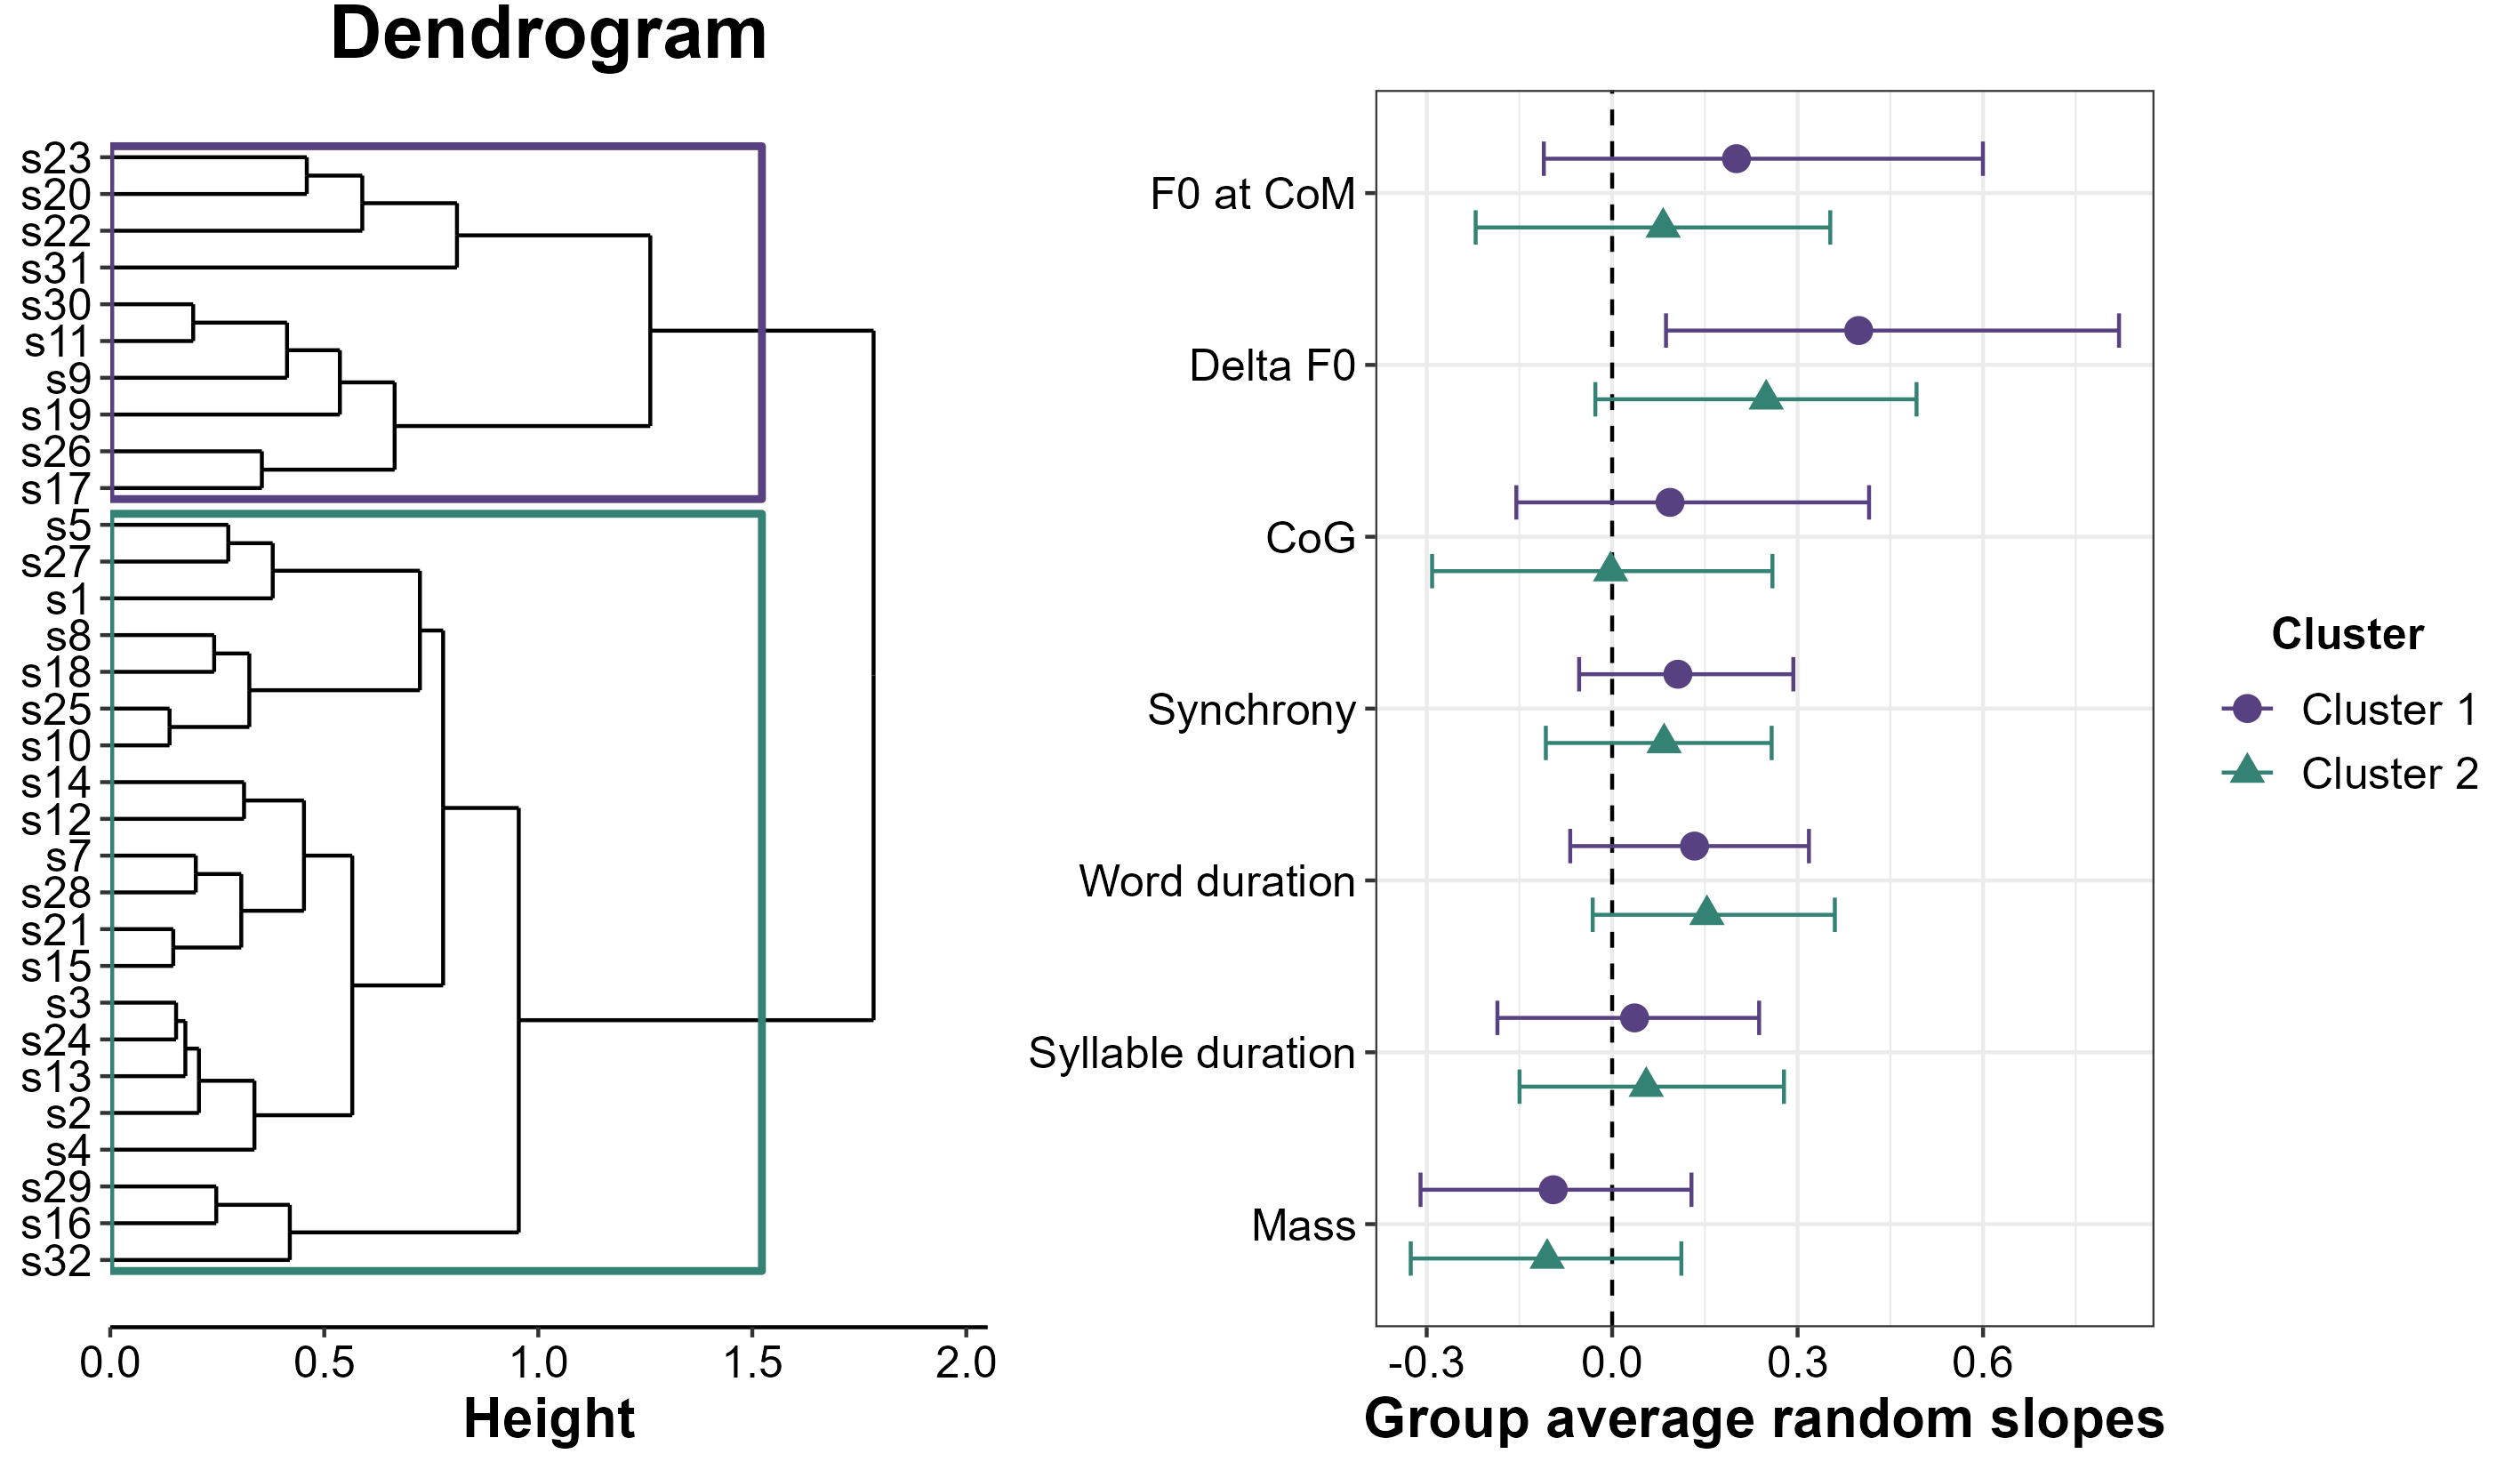
\includegraphics[width=\textwidth]{s1_clusters}
	\caption{Results of cluster analysis. Left: Dendrogram showing cluster affiliations of all speakers. Right: Plot showing the group averages and 90\% CrIs per cluster for each prosodic parameter.}
	\label{fig:s1_clusters}
\end{figure}

In order to illustrate what characterizes these clusters, Figure \ref{fig:s1_clusters} (right) shows the group averages and 90\% CrIs of the random slope coefficients for every parameter per cluster, thus visualizing the differences and similarities between the clusters. A positive value here indicates that a parameter has higher values in the new than in the accessible referents, i.e., that the parameter is used in the expected direction, marking new referents as more prominent than accessible ones. As evident from this plot, Cluster 1 appears to mark information status more strongly than Cluster 2 in terms of the four F0-related parameters F0 at CoM, Delta F0, CoG, and synchrony. Regarding word and syllable duration, the relation is reversed with Cluster 2 producing slightly larger differences between new and accessible than Cluster 1. However, it should be noted that especially for syllable duration, the differences between new and accessible referents are very small with a mean close to zero for both clusters. 

The cluster analysis gives an approximation as to what may be the main distinguishing factor between groups of speakers, namely, the strength of encoding of information status. Nevertheless, overall, the two clusters are remarkably similar, Delta F0 being the most important parameter for both groups of speakers. However, the cluster analysis coarsely groups speakers together and thus is not able to capture the full extent of individual variability that was observed in the descriptive analysis above. The implications of the choice of methodology for looking at individual variability will be further discussed in Section \ref{sec:Production 1 discussion} below.

To integrate observations of how speakers differ in their usage of continuous phonetic cues to information status on the one hand and categorical phonological cues on the other, Figure \ref{fig:s1_statustype_bycluster} plots the number of speakers in a cluster by whether they use accent status and accent type in the expected direction to encode information status, i.e., produce more nuclear and more prominent pitch accents in new than in accessible referents. Most of the speakers in Cluster 1 do not use accent status as a cue to information status. In Cluster 2, by contrast, there is a relatively even split into speakers who use accent status and speakers who do not. As a reminder, Cluster 1 includes the speakers that use the continuous phonetic measures (at least those related to F0) more strongly to encode information status than those in Cluster 2. Somewhat unexpectedly, the distribution of speakers who do or do not use accent status as a cue to information status suggests the reverse, namely, that Cluster 2 more strongly marks information status via prosodic structure. However, there was also a very subtle trend for speakers in Cluster 2 to use duration more effectively than those in Cluster 1. Cluster 2 could thus be regarded as a group of speakers that are more reliant on aspects related to timing, encompassing both accent status and duration, to mark information status.

By contrast, the results regarding accent type usage (see Figure \ref{fig:s1_statustype_bycluster}) seem to be in line with the strong versus weak encoders split observed with regard to the continuous prosodic parameters: All speakers in Cluster 1 (the strong phonetic encoders) use accent type in at least one position (Word1 or Word2) to mark information status, while in Cluster 2, seven speakers do not use accent type at all. What is more, half of the speakers in Cluster 1 use accent type as a cue in both positions, while only a quarter of speakers in Cluster 2 do the same. Accent type thus reflects the findings with regard to the continuous parameters emerging from the cluster analysis. Or, conversely, the continuous F0-related parameters are able to adequately capture aspects characterizing accent type categories. 

\begin{figure}
	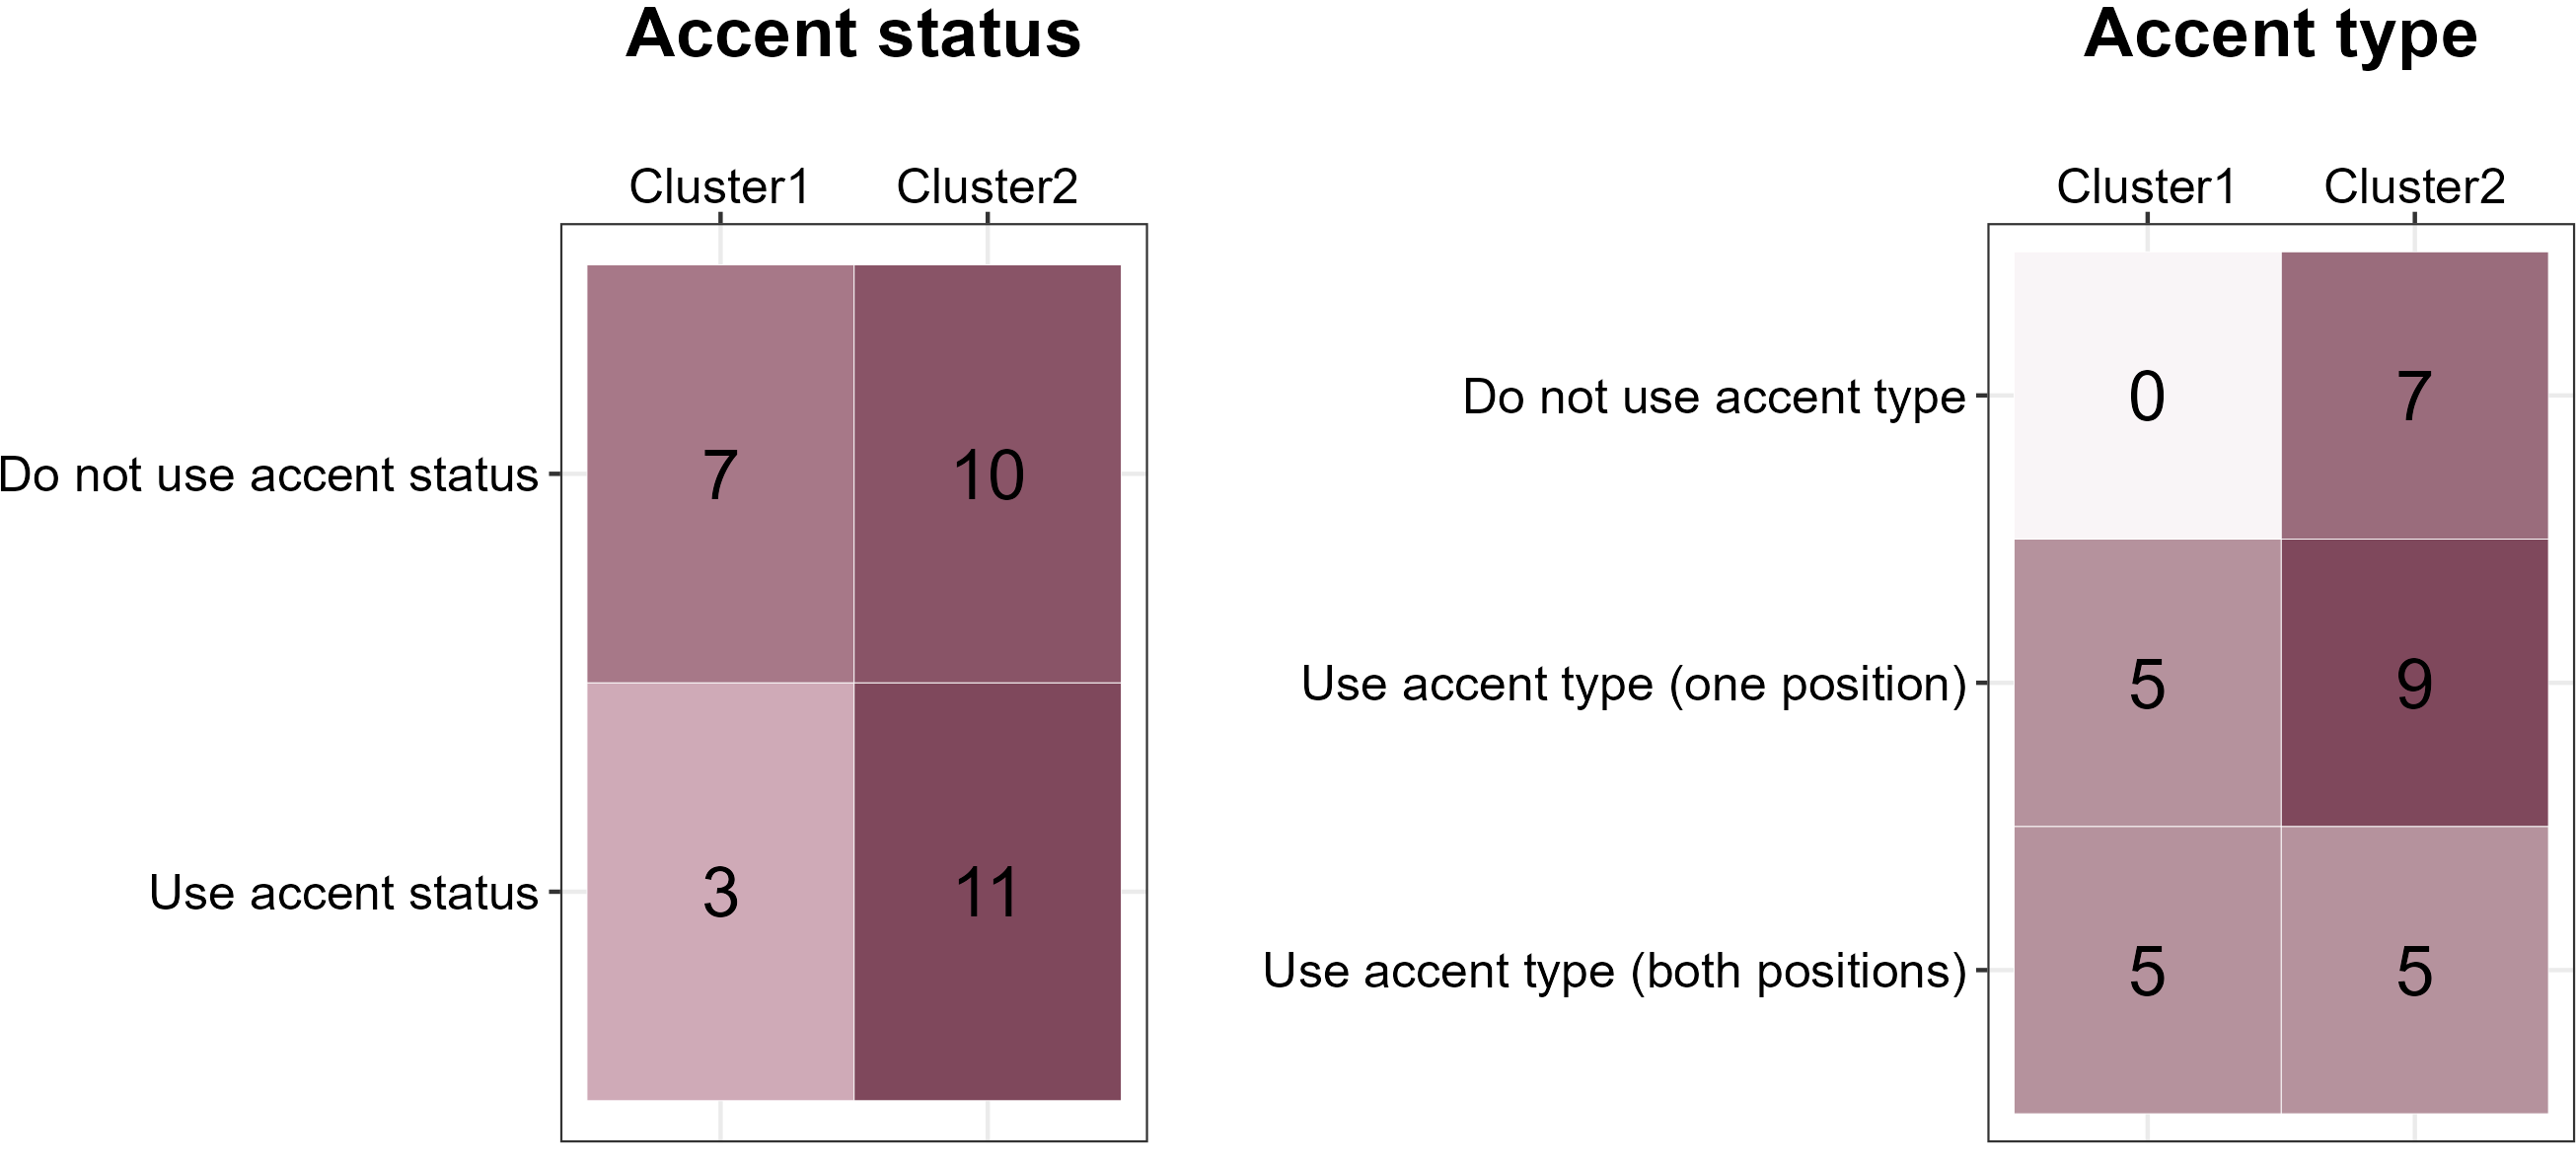
\includegraphics[width=\textwidth]{s1_accent_statustype_bycluster_cropped}
	\caption{Plot showing the number of speakers using accent status in Word1 (left) and accent type (right) to encode information status as a function of the cluster they belong in.}
	\label{fig:s1_statustype_bycluster}
\end{figure}

For completeness, a brief note on sociodemographic characteristics of the two clusters is in order. Since this is not the primary objective of the present study, we can only characterize the speakers in terms of their age, gender, and region of origin (see Table \ref{table:s1_sociodemographics}). Speakers associated with Cluster 1 are slightly older than those associated with Cluster 2, although the difference is only three years. The gender distribution is relatively balanced across clusters: 70\% of speakers in Cluster 1 are female compared to 76\% of speakers in Cluster 2. Finally, speakers in Cluster 1 are more likely to originate from the south of Germany (Bavaria, Baden-Wuerttemberg, and Thuringia) than speakers in Cluster 2, where 57\% of speakers are from the north (Lower Saxony, Schleswig-Holstein, Hamburg, and North Rhine-Westphalia). Generally, these observations reflect the relatively uniform age group from which participants were recruited and the skewed gender balance. In light of these shortcomings and the lack of clear tendencies, we will return to the examination of potential sociodemographic effects in the General Discussion (Chapter \ref{ch: general discussion}) after having added further data points in the following two studies.

\begin{table}[]
\begin{tabular}{lrr}
\lsptoprule
                 & Cluster 1 \newline n = 10    & Cluster 2 \newline n = 21    \\
                 \midrule
Age (median)     & 28                     & 25                     \\
Gender           & 70\% female, 30\% male & 76\% female, 24\% male \\
Region of origin & 30\% north, 70\% south & 57\% north, 43\% south \\
\lspbottomrule
\end{tabular}
\caption{Sociodemographic characteristics of the two clusters.}
\label{table:s1_sociodemographics}
\end{table}

\section{Interim discussion} \label{sec:Production 1 discussion}

Across speakers, Delta F0 emerged as the strongest correlate of information status in our data, new referents being produced on average with higher Delta F0 than accessible referents. In addition, new referents were reliably produced with more prominent accent types and there was a strong tendency for new referents (in Word1) to be realized with a nuclear as opposed to a prenuclear accent. There was also some evidence that F0 at CoM, synchrony, and word duration play a role in information status marking, which was, however, modulated by position in the sentence: New referents in Word1 were produced with on average higher F0 at CoM than accessible referents, new referents were on average longer than accessible ones, more so in Word1 than in Word2, and had higher synchrony values, particularly in Word2. CoG, syllable duration, and periodic energy mass were of little to no importance in the encoding of information status. The overall results on the group level are generally reflected on the individual level, with Delta F0 being the cue used by most speakers (25 out of 32). This finding underlines the predominance of F0 as a correlate of prominence \citep[e.g.,][]{bolingerTheoryPitchAccent1958, fryExperimentsPerceptionStress1958, liebermanAcousticCorrelatesWord1960, baumannWhatMakesWord2018, roessigTracingPhoneticSpace2022} not only in averaged data but also for the individual speaker.

As per the cluster analysis performed on the models' random slopes, speakers were very similar in their encoding of information status, particularly in the direction of effects observed for all seven prosodic parameters. Nevertheless, the cluster analysis revealed a split into two groups, each employing a slightly distinct strategy. The main difference between these two strategies lies in the extent to which speakers modulated any given parameter, i.e., the strength of encoding: Cluster 1 (consisting of fewer speakers) marked a larger difference between new and accessible target words than Cluster 2 (the larger cluster of the two). These results are in line with previous findings that some speakers encode certain pragmatic contrasts more effectively than others \citep[e.g.,][]{cangemiListenerSpecificPerceptionSpeakerSpecific2015}. Such speakers are either better communicators who consciously (or unconsciously) mark pragmatic contrasts (such as newness) more clearly in order to facilitate interpretation of utterances on the side of the listener or they are more sensitive to such pragmatic contrasts which enables them to mark them prosodically.

Especially in perception studies, higher sensitivity to pragmatic contrasts encoded via prosody has been linked to concepts such as pragmatic/communicative skill or empathy \citep{bishopPhonologyPhoneticsSignalextrinsic2020, orricoInfluenceEmpathyAutisticlike2023}. Analogously, in production, speakers with higher pragmatic skill or empathy would be expected to encode pragmatic contrasts more strongly than speakers with lower pragmatic skill, which could explain the difference in strength of encoding observed in our data. However, recent production studies investigating the relation between pragmatic skill and contrastiveness of categories find only subtle if not inconclusive effects \citep{turnbullListenerorientedPhoneticReduction2019, bishopBriefReportAutistic2022}.

Beyond the difference in the strength of encoding of information status, we found more diverse strategies on the individual level in the choice of parameters used to encode information status when considering the raw data. One potential reason enabling this variability is the acoustic redundancy that is present in the signal. In West Germanic languages, prosodic prominence is encoded via the F0 contour, duration, and intensity and it is assumed that all three acoustic dimensions play a role in the prosodic marking of pragmatic contrasts, such as information status. Functional redundancy in speech ensures the robustness of the message and guarantees communicative success in noisy situations \citep{winterSpokenLanguageAchieves2014}. This opens up the possibility for individual speakers to make use of only some of the available prosodic parameters without losing the ability to successfully encode the intended meaning. In our data, there are speakers who rely solely on F0-related cues, while others use only changes in duration to encode information status, thus efficiently exploiting the functional redundancy in the signal. In fact, speakers rarely make use of the full range of cues available to them. Out of our 32 speakers, only one encodes information status maximally redundantly. Similar ``cue-trading" effects have also been observed in \citet{severijnenYourVOORnaamNot2024} in the encoding of word-level stress in Dutch, where speakers who used higher mean F0 to mark stress were less likely to rely on intensity.

Integrating the continuous and categorical results at the individual level revealed a surprising asymmetry: While the strong phonetic encoders were also more likely to use accent type as a cue to information status than the weaker encoders, the relation was reversed for accent status. Weaker phonetic encoders, who showed a slightly stronger preference for using duration, were more likely to use accent status than stronger phonetic encoders (but note again that accent status can only be used as a cue in Word1, since Word2 is always produced with a nuclear accent). Speakers may split into those who modify timing (including accent status) and those that modify the shape of the F0 contour, which is reflected in both accent type choice and the phonetic parameters measuring F0. Interestingly, this split reflects the dichotomy between metrical structure (or relative prominence) and tune (or pitch) that lies at the heart of influential theories of intonational phonology (e.g., \citealt{laddIntonationalPhonology2008}, see also Section \ref{section: structural prominence}). Metrical structure describes the alternation of strong and weak entities at the sentence level, while tune refers to the alternation of rises and falls in the F0 contour. These two aspects are orthogonal to each other and are independently variable \citep{laddIntonationalPhonology2008}. In the present data, accent status and duration are manifestations of metrical structure that are used to encode information status by the same group of speakers, while accent type and the continuous F0 measures capture variability in the tune. The results may suggest that not only are tune and metrical structure independently manipulable, but that individual speakers may have preferences regarding which of the two aspects they modify to encode a semantic-pragmatic contrast, such as information status. This hypothesis will be further discussed in Chapter \ref{ch: general discussion}. 

Arguably, a change in metrical structure should be more consequential for the listener than F0 modulations, as it has been shown in previous studies that accent status is among the most important cues to the perception of prominence \citep{baumannWhatMakesWord2018}. Thus, when it comes to perception, the group of speakers modifying accent status might emerge as the overall stronger encoders than the group that use accent type and F0-related parameters to a larger extent to encode information status. However, our study lacks variability in the likely most important categorical prosodic cue to prominence, i.e., the presence or absence of a pitch accent \citep[e.g.,][]{baumannWhatMakesWord2018, wagnerExploitingSpeechgestureLink2019}, since all of our target words were accented. Speakers that use accent status as a cue to the accessible-new contrast could also be more likely to vary accentuation patterns in marking other pragmatic contrasts (e.g., a given-new contrast), which would make them more successful in communicative settings than the accent type and F0 encoders. This is a matter for further investigation.

In the present study, we investigated individual variability via two different approaches: Descriptively, by examining the distributions of the prosodic parameters for each speaker and by performing a cluster analysis on the random slope coefficients of mixed-effects models. These approaches differ substantially and emphasize different aspects in the study of inter-speaker variability. While the cluster analysis aims to identify common strategies shared by multiple speakers in an objective manner, the descriptive method allows for an in-depth exploration of every single speaker. Crucially, the cluster analysis method is fairly conservative in estimating differences across speakers, instead emphasizing similarities. This is a consequence of using random slope coefficients as input for the clustering. Random slopes account for by-speaker variation in the effect of a predictor \citep[e.g.,][]{winterStatisticsLinguistsIntroduction2020}, in our case information status. However, random slopes are not estimated independently for each individual but always together with and in relation to the group-level estimates. This means that the by-speaker estimates are drawn towards the overall mean effect, a process known as ``shrinkage" \citep[271-272]{winterStatisticsLinguistsIntroduction2020}. Nevertheless, the cluster analysis provides valuable insight into different strategies employed by groups of speakers in a manageable, straightforward-to-interpret way. The descriptive exploration, by contrast, reveals that there are more diverse strategies in the data than the cluster analysis suggests. However, this may over-emphasize individual variability, especially in the light of relatively few data points per speaker, which is arguably the case in our data set. Running the cluster analysis on the ``shrunken" random slope estimates thus gives the results more statistical validity. Much can therefore be gained by considering insights from both approaches.

The present chapter has provided an exploratory account of individual differences and similarities in the prosodic marking of information status. However, several questions remain unanswered. As has already been shown by \citet{cangemiListenerSpecificPerceptionSpeakerSpecific2015}, more redundant prosodic encoding of pragmatic contrasts facilitates their interpretation on the side of the listener. However, it remains unclear how the listener deals with contradictory cues. For example, there are cases in our data where a speaker produces new words on average with longer duration than accessible ones, yet accessible words exhibit more extensive F0 rises (or vice versa).

Furthermore, this study describes the nature of inter-speaker variability but provides no potential causes of them. In a further study, we will consider communicative skill as a potential predictor of individual differences, which has previously yielded promising results, particularly in perception studies \citep{bishopPhonologyPhoneticsSignalextrinsic2020, orricoInfluenceEmpathyAutisticlike2023}. Finally, the present study considered only information status as a factor to be encoded via prosodic prominence. We will expand on this by taking into account other (semantic-pragmatic and syntactic) factors to see whether comparable patterns of across-speaker differences and similarities emerge in their encoding via prosodic prominence. Chapter \ref{ch:Production II} aims to address some of these issues.

\chapter{Production II: Individual variability in the encoding of lexical and referential givenness, grammatical role, and sentence position} \label{ch:Production II}
\chaptermark{Production study II}

\section{Overview}

In this chapter, we investigate inter-individual variability in the prosodic encoding of lexical and referential givenness (or information status) as well as the syntactic factors grammatical role and sentence position. Building on the findings of the first production experiment presented in Chapter \ref{ch:Production I}, the present study thus considers more factors that influence prominence production and are potentially marked differently across speakers. Using a similar method as in the first study, we scrutinize the extent and form of individual variability in production data collected in an interactive reading task. In addition, the role of communicative skill will be explored as a potential reason for any emerging individual differences.

In our first production experiment, reported in Chapter \ref{ch:Production I}, we considered an integrated concept of information status as a prominence-influencing factor and individual variability that emerged in its prosodic encoding. The present study takes a different approach that allows for the separate investigation of two dimensions of information status that have been shown to influence prosodic prominence: lexical and referential information status \citep{baumannReferentialLexicalGivenness2012, baumannCoreferenceLexicalGivenness2013, riesterRefLexSchemeAnnotation2017}. Following the RefLex annotation scheme \citep{riesterRefLexSchemeAnnotation2017}, we understand lexical givenness as relating to the number of and distance between mentions of a lexical item. When a lexical item is mentioned for the first time, it can be regarded as lexically new (l-new). In any repeated mentions within the next five intonation phrases, it is lexically given (l-given), no matter if it is coreferential with the first mention or not \citep[24]{baumannCoreferenceLexicalGivenness2013}. Referential givenness, by contrast, is determined by coreference. If an entity is first introduced to the discourse, it is referentially new (r-new), any following entities that are coreferential with their antecedent are referentially given (r-given). Although intermediate levels of givenness exist for both the lexical and the referential dimension \citep[e.g.,][]{riesterRefLexSchemeAnnotation2017}, we restrict ourselves here to the two end points of each scale, new and given. We thus increase the contrast of the information status manipulation in comparison to the new-accessible contrast investigated in the first experiment, where the new condition encompassed both lexical and referential newness and the accessible condition represented an intermediate level of r-bridging and l-accessible information. Both lexical and referential givenness are expected to influence prosodic prominence production, in that l-newness and r-newness should increase prosodic prominence and l-givenness as well as r-givenness should decrease it \citep{baumannReferentialLexicalGivenness2012, baumannCoreferenceLexicalGivenness2013}. However, it is unclear whether the lexical and referential dimensions are encoded by speakers to a similar extent or whether some speakers encode primarily the lexical dimension while others focus more on the referential dimension. 

Furthermore, we add two syntactic factors to our investigation, namely grammatical role and sentence position. We are interested in whether and how speakers differ in their prosodic productions influenced by these two factors. While grammatical role and sentence position are not encoded via prosodic prominence in the same way as information status, they may nevertheless influence a word's prosodic realization. Grammatical role interacts with information structure in that subjects often denote discourse-important information \citep{arnoldReferenceFormDiscourse1998}, which is prosodically attenuated. Conversely, the object role is often occupied by new information that is prosodically highlighted \citep{hallidayNotesTransitivityTheme1967, terkenDeaccentuationWordsRepresenting1994}.

There is also an interaction between grammatical role and sentence position, in that subjects tend to occur sentence-initially \citep{himmelmannProminenceProsodyFirst2015}, while objects occur later in the sentence. Prosodically, the nuclear accent, i.e., the most prominent accent, is likely to be realized on the object as the final argument  \citep{griceGermanIntonationAutosegmentalMetrical2005}. Sentence-initial subjects, by contrast, are unlikely to receive a nuclear accent in unmarked utterances \citep{feryGermanIntonationalPatterns1993}. However, the initial position often attracts a prenuclear accent, which is structurally less prominent but can be phonetically very prominent, e.g., steeply rising \citep{baumannInfluenceInformativenessProsody2021}. Conflicting assumptions could thus be derived from these previous findings. However, we assume that metrical structure prevails, so that we expect grammatical objects and words in the medial sentence position to be produced more prominently than subjects and words in the initial position. Nevertheless, individual speakers may differ in their mapping of prosodic prominence to syntactic functions.

As discussed in Chapter \ref{ch:background variability}, many previous studies have observed substantial individual variability in the production of prosodic prominence. Although several studies note that there are inter-individual differences, few production studies investigate reasons behind this variability. Previous perception experiments, however, have found a correlation between the processing of prosodic prominence and communicative skill \citep[e.g.,][]{bishopPhonologyPhoneticsSignalextrinsic2020, orricoInfluenceEmpathyAutisticlike2023}. These studies generally observed that listeners with lower communicative skill were less sensitive to the prosody-meaning mapping. We will explore whether such an effect can also be found in the production of prosodic prominence as it is used to encode several semantic-pragmatic and syntactic properties. To quantify communicative skill, we employed a subset of the Autism Spectrum Quotient questionnaire \citep{baron-cohenAutismSpectrumQuotientAQ2006}, i.e., ten questions asking participants to self-rate their communicative skill. This set of questions has proven useful in previous studies with similar research aims \citep[e.g.][]{bishopPhonologyPhoneticsSignalextrinsic2020} and constitutes a straightforward and convenient way to assess communicative skill. Following findings in previous perception studies, we expect speakers with higher communicative skill to show a clearer mapping of prosody to meaning, i.e., to produce larger prosodic contrasts between the distinct levels of each semantic-pragmatic and syntactic variable we investigate.

In the present study, we ask how speakers differ in their prosodic marking of lexical and referential givenness, grammatical role, and sentence position and whether any observed differences relate to communicative skill. To address these questions, we collected production data in a reading task along with information on the communicative skill of our participants. Results suggest that the extent of variability differs across the four factors we manipulated, with the overall most strongly encoded variable sentence position giving rise to the most variability. Nevertheless, we find speaker-specific encoding strategies across all four factors, which relate to the choice of prosodic parameters that encode a certain contrast as well as the extent to which a certain cue is used. Furthermore, we observe mostly positive correlations between communicative skill and the produced contrast between levels of lexical givenness, grammatical role, and sentence position, but predominantly negative correlations for referential givenness.

In Section \ref{sec:Production2 methods}, we describe in detail the process of data collection, processing, and analysis. Section \ref{sec:Production2 results} presents the results of this study, focusing on both group and individual level. Finally, Section \ref{sec:Production2 discussion} constitutes a brief discussion of the findings in the context of previous literature. The data collection process and averaged results across speakers have previously been reported in \citet{baumannBoostingInhibitingHow2024}. A preliminary analysis of individual differences in a subset of the data using partially different prosodic parameters has been presented in \citet{lorenzenDoesCommunicativeSkill2024}.

\section{Methods} \label{sec:Production2 methods}

\subsection{Reading materials, procedure, and participants}

We collected production data via an interactive reading task. Reading material consisted of eight short stories, each containing one target word occurring in five different conditions. An example story (with English translation) is provided in \ref{itm:story_banane}. The full list of stories is available in Appendix \ref{Appendix B}. All target words are stressed on the penultimate syllable and associated with comparable lexical frequencies according to the \textit{Wortschatz Leipzig} corpus (\url{https://corpora.uni-leipzig.de/de/res?corpusId=deu_news_2022}). The target words were manipulated with regard to the four factors lexical givenness, referential givenness, grammatical role, and position in the sentence, each of which has two levels.
Target 1 is lexically new (l-new), all subsequent target words are lexically given (l-given). Targets 1 and 4 are referentially new (r-new), all others are referentially given (r-given). Targets 2, 3, and 5 refer to the same entity as Target 1, while Target 4 introduces a different referent into the story. Referential givenness is marked by definiteness in the article, with the r-new words marked by indefinite articles and the r-given words by definite articles.\footnote{Note that there is no instance of an l-new but r-given target word because this would entail using a different lexical item. We deemed it crucial to keep the lexical item constant in order to compare the prosodic form across different conditions.} Regarding the syntax of the target utterances, most words are in the grammatical object role, only Target 3 is a subject. Finally, Targets 1, 2, and 4 occur in a medial position followed only by a verb, while Targets 3 and 5 are in the initial position of a sentence. Table \ref{table:summary_manipulations} summarizes the conditions for each target word.

\begin{enumerate}[resume*]
\item \label{itm:story_banane} \textit{Schon seit vielen Jahren arbeitet Susanne im Zoo als Tierpflegerin. Dort ist sie sehr glücklich und kümmert sich liebevoll um alle ihre Schützlinge. Heute hat Susanne \textbf{eine Banane} (Target 1) mitgebracht. Sie hatte eine große Kiste mit viel Obst und Gemüse dabei und besonders die Affen waren ganz aufgeregt. Dann hat Susanne \textbf{die Banane} (Target 2) herausgeholt. Sofort versammelten sich die Affen um sie. \textbf{Die Banane} (Target 3) sah richtig lecker aus und der kleine Affe Tobi wollte sie unbedingt haben. Erst vor ein paar Tagen hatte ein Mädchen mit seinen Eltern vor dem Affengehege gestanden und Tobi beobachtet. Dabei hat das Mädchen \textbf{eine Banane} (Target 4) gegessen. Da konnte Tobi die schöne gelbe Frucht nur ansehen, aber jetzt will er endlich eine probieren! \textbf{Die Banane} (Target 5) wird er bestimmt sehr genießen.}

Susanne has been working as an animal keeper at the zoo for many years. She is very happy there and lovingly looks after all her charges. Today Susanne brought \textbf{a banana} (Target 1) with her. She had brought a big box with lots of fruit and vegetables, and especially the monkeys were very excited. Then Susanne took out \textbf{the banana} (Target 2). The monkeys immediately gathered around her. \textbf{The banana} (Target 3) looked really tasty and little monkey Tobi desperately wanted to have it. Just a few days ago, a girl and her parents had been standing in front of the monkey enclosure watching Tobi. In doing so, the girl ate \textbf{a banana} (Target 4). Tobi could only look at the beautiful yellow fruit, but now he finally wants to try one! He will definitely enjoy \textbf{the banana} (Target 5) a lot.
\end{enumerate}

\begin{table}[]
\begin{tabular}{llllll}
\lsptoprule
Target                & (1) & (2) & (3) & (4) & (5) \\ \hline
Lexical givenness     & l-new               & l-given              & l-given               & l-given              & l-given              \\
Referential givenness & r-new               & r-given              & r-given               & r-new                & r-given              \\
Grammatical role      & object              & object               & subject               & object               & object               \\
Sentence position              & medial              & medial               & initial               & medial               & initial              \\
\lspbottomrule
\end{tabular}
\caption{Summary of the four factors manipulated in each target word.}
\label{table:summary_manipulations}
\end{table}

The recordings were conducted at the phonetics institute at the University of Cologne. Participants were sat in a sound-attenuated recording booth wearing a head-mounted AKG C544L condenser microphone. The speech signal was recorded on a computer via Adobe Audition at a sampling rate of 44.1 kHz and a bit depth of 16 bit. The stories were presented to the speakers on a monitor in a PowerPoint presentation that they were able to control via a keyboard. Each story was accompanied by an illustration in order to give the task a more interesting and playful nature (see Figure \ref{fig:banane} for the picture corresponding to the example story presented in \ref{itm:story_banane} above). In addition to the experimenter and the participant, a confederate was present at each recording session, who sat outside the recording booth but was visible to the participant through a window. 

\begin{figure}
		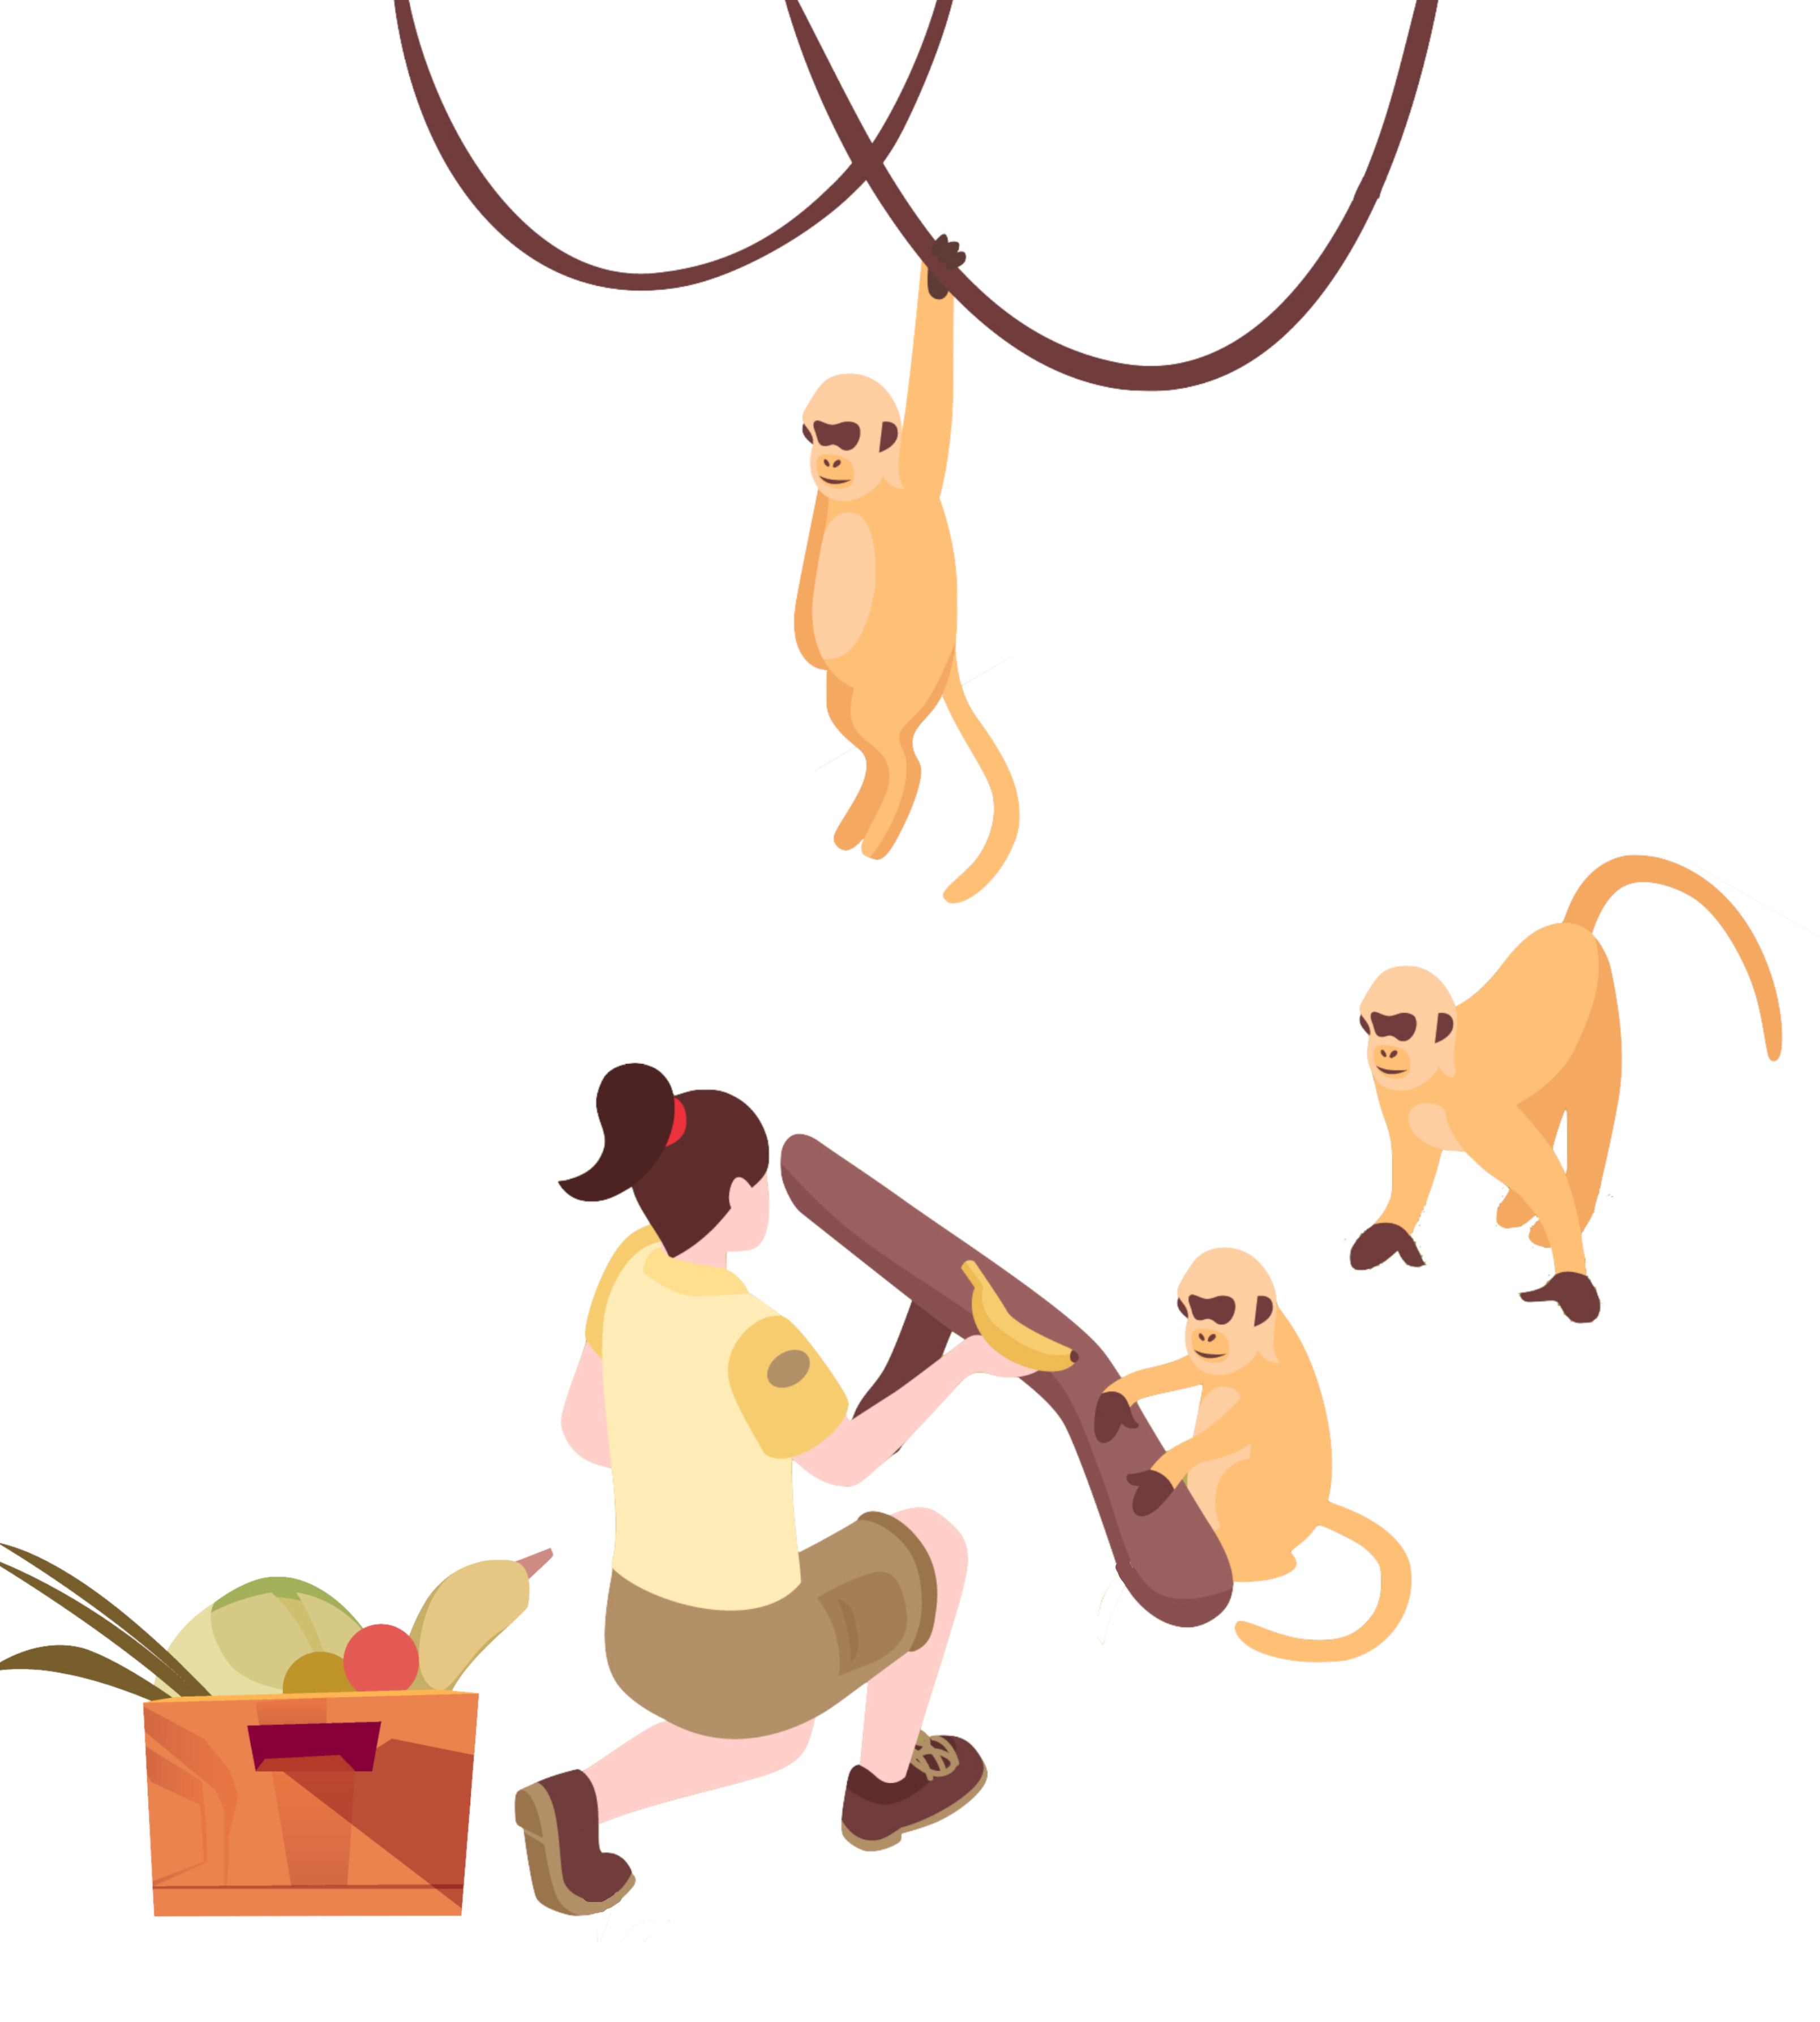
\includegraphics[scale = 0.05]{banane}
	\caption{Picture accompanying the example story in \ref{itm:story_banane}.}
	\label{fig:banane}
\end{figure}

The participant was asked to first read each story quietly and then aloud for the confederate in such a way that they would be able to memorize it. After the participant had finished reading the story, the confederate answered three comprehension questions, which were also read to them by the participant. The confederate answered these questions in written form and the participant did not see these answers at any point during the recording session. This set-up was intended to foster the participant's engagement with the reading task and thus prevent monotonous speech.

Each participant read two practice stories before the actual task began. The eight stories were then read by the participant in pseudo-randomized order. A recording session lasted approximately 30 minutes. Prior to the recording, participants gave informed consent to participate in this experiment and they received a monetary compensation of eight euros after completing the experiment. After the reading task, participants completed a questionnaire providing sociodemographic information, i.e., their age, place of birth, and native language(s). In addition, participants rated their communicative skill on ten scales, i.e., a subset of the questionnaire designed by \citet{baron-cohenAutismSpectrumQuotientAQ2006}. Questions included, for example, whether they enjoy small talk and if they can tell when it is their turn to talk. The full questionnaire is provided in Appendix \ref{Appendix B}. Participants could receive up to one point per scale for an overall score of 0 to 10 points, where 0 indicates very low and 10 very high communicative skill.\footnote{Note that this scoring system is the inverse of the original scoring system by \citet{baron-cohenAutismSpectrumQuotientAQ2006}, which has been used as a diagnostic tool for autism.}

We recorded 20 native speakers of German, of which one failed to complete the questionnaire, so that we will report on 19 speakers in the analyses including communicative skill as a variable. Participants were between 18 and 31 years old (mean = 25, SD = 3.9), 13 participants identified as female, six as male. They grew up in seven federal states of Germany but spoke no clearly discernible dialect and all were living in and around Cologne at the time of recording. No participant reported a diagnosed speech or hearing impairment. 

\subsection{Data, annotation, and measurements} \label{section: measurements study2}

Each participant produced 40 target utterances (8 stories x 5 target words) for a total of 800 target utterances. We excluded eleven utterances due to hesitations or slips of the tongue, so that 789 utterances entered the analysis. Utterances were automatically segmented using WebMAUS \citep{schielAutomaticPhoneticTranscription1999, kislerMultilingualProcessingSpeech2017} and segment boundaries were manually corrected in Praat \citep{boersmaPraatDoingPhonetics2023}. Phrase boundaries and tonal events were then annotated by two trained annotators independently following the DIMA guidelines \citep{kuglerDeutscheIntonationModellierung2022}.\footnote{Inter-rater agreement was 93\% for the boundary tier and 68\% for the tonal tier.} In cases of disagreement, a consensus annotation was reached by consulting another expert. Accent status was determined with reference to position in the sentence and phrase boundary presence, i.e., target words without a pitch accent were classified as ``deaccented", target words carrying the final pitch accent in an intermediate phrase were classified as ``nuclear" and those carrying a non-final pitch accent as ``prenuclear". Annotations on the tonal tier were translated into GToBI pitch accent types \citep{griceGermanIntonationAutosegmentalMetrical2005}.\footnote{Inter-rater agreement was 62\% for the GToBI annotations. Note that this number is considerably lower than in Production Study I, since the DIMA and GToBI labels were assigned simultaneously this time, while GToBI labels were based on a consensus DIMA annotation in Study I.}

To establish comparability with the previous production study presented in Chapter \ref{ch:Production I}, we extracted the same prosodic parameters. The only exception is the addition of intensity here, which we decided to forego in the first production study due to the lack of control over microphone quality and position. We thus collected eight prosodic measures, i.e., F0 at the Center of Mass (F0 at CoM), Delta F0, Center of Gravity (CoG), synchrony, word and syllable duration, intensity, and periodic energy mass. The first four prosodic parameters, capturing different aspects of the F0 contour, as well as the periodic energy mass measure were derived via the ProPer toolbox (\citealt{albertModelSonorityBased2023}, see Sections \ref{section: prominence form} and \ref{section: measurements study1} for further details). After determining the Center of Mass (CoM) in the stressed syllable of the target word, F0 at CoM  was measured in semitones relative to a low baseline determined individually for each speaker to capture the general scaling of this syllable. To more dynamically capture F0 change, we took the difference of F0 at the CoM of the stressed syllable and the CoM of the preceding syllable in semitones. As a measure of alignment, we determined the CoG in the stressed syllable relative to the beginning of the word and normalized by word duration. Finally, synchrony quantifies the distance between the CoM and the CoG, thus providing information about the shape of the F0 contour over the stressed syllable.

To capture timing and intensity, we measured the duration of each target word as well as the duration of the stressed syllable (i.e., the penultimate syllable) of each target word in milliseconds. Intensity was measured as the mean of the intensity curve in the stressed syllable in dB. Finally, periodic energy mass was measured as the area under the periodic energy curve associated with the stressed syllable. Periodic energy mass is reported as a unitless measure centered around 1. In the statistic analysis of word duration, syllable duration, and periodic energy mass, we excluded phrase-final target words to ensure that any observed effects are not the result of phrase-final lengthening.

\subsection{Statistical analysis} \label{sec:Production2 statistics}

All statistical analyses were conducted in R \citep{rcoreteamLanguageEnvironmentStatistical2022}. For data wrangling and visualization, we used the \pkg{tidyverse} \citep{wickhamWelcomeTidyverse2019}, \pkg{cowplot} \citep{wilkeCowplotStreamlinedPlot2020}, and \pkg{ggh4x} \citep{vandenbrandGgh4xHacksGgplot22024} packages. We ran Bayesian regression models using the \pkg{brms} package \citep{burknerBrmsPackageBayesian2017} as an interface to the Stan modeling language \citep{carpenterStanProbabilisticProgramming2017}. The package \pkg{cluster} was used for cluster analyses \citep{maechlerClusterClusterAnalysis2022} and we used \pkg{ggdendro} \citep{devriesGgdendroCreateDendrograms2024} to create the dendrograms. Data and analysis scripts are available online (\url{https://osf.io/m5xwe/}).

We ran ten Bayesian mixed-effects regression models, one for each prosodic parameter under investigation. For the categorical parameters, we ran two cumulative models with accent status (ordered levels from most to least prominent: nuclear > prenuclear > deaccented) and accent type (ordered levels: L+H* > L*+H > H* > H+!H* > H+L* > !H* > L*, following \citealt{baumannPerceptualProminencePitch2015}) as the respective dependent variables. The continuous parameters were z-scored before entering the statistical analysis as the dependent variables in the respective models. Each model contained lexical and referential givenness, grammatical role, and sentence position as well as communicative skill as predictors and the interactions of the four manipulated variables with communicative skill. The communicative skill variable was centered by subtracting the mean from each value. This serves to make the model parameters interpretable with regard to the mean communicative score, which is most representative for our sample of speakers. In addition, we included random intercepts for speaker and item, and the by-speaker and by-item random slopes for lexical and referential givenness, grammatical role, and sentence position. Four sampling chains ran for 4,000 iterations with a warm-up period of 2,000 iterations, yielding a total of 8,000 posterior samples per model. We used a weakly informative, normally distributed prior with a mean of zero and a standard deviation of one for the regression coefficients and default priors supplied by \pkg{brms} for the remaining parameters. Model fits were assessed visually by inspecting the posterior predictive checks and by ensuring that no model yielded Rhat values larger than one. 

For each model, we report the regression coefficient $\beta$ and 90\% credible intervals (CrIs) under the posterior distributions as well as the posterior probability that $\beta$ is larger than zero: Pr($\beta$\textgreater{}0). Similar to the analysis presented in Chapter \ref{ch:Production I}, we consider the effect of a predictor variable reliable if the 90\% credible interval (CrI) does not include 0 and the probability that $\beta$ is larger than zero is higher than 0.95 or lower than 0.05. 

To investigate inter-individual differences in the encoding of all four semantic-pragmatic and syntactic variables, we utilized the by-speaker random slopes from the models run on the continuous prosodic parameters following \citet{baumannWhatMakesWord2018}.
By-speaker random slopes account for speaker-specific behavior differing from the group average. To identify speakers employing the same common strategies, we ran hierarchical cluster analyses on the extracted random slope values (see Section \ref{sec: stats study1} for more technical details on this analysis). The number of clusters is determined by the greatest average silhouette width, which gives an indication to the well-formedness of clusters \citep[see][]{levshinaHowLinguisticsData2015}. Silhouette width values range from 0 to 1, where a value above 0.25 indicates that there is potential for clustering in the data \citep[88]{kaufmanFindingGroupsData1990}.

\section{Results} \label{sec:Production2 results}

\subsection{Overall results} \label{sec:Production2 overall results}

In this section, we first consider the average results across all speakers. Figure \ref{fig:s2_accent_statustype} illustrates accent status and accent types produced in each of the five different target word conditions. In terms of accent status, each target word can be produced with a prenuclear or nuclear accent, while deaccentuation is rare overall and confined to Targets 2 and 4, the lexically given medial objects.\footnote{Note that there is one instance of deaccentuation in Target 5, where a speaker produced a contrastive accent on the preceding article, which seems to be an exceptional pattern.} Target 1 (the lexically and referentially new medial object) mostly receives a nuclear accent (about 96\%). Target 4 (the lexically given but referentially new medial object) is also predominantly produced with a nuclear accent (in about 75\% of cases), while Target 2 is more likely to receive a prenuclear accent (76\%). In cases of deaccented or prenuclear-accented medial objects, the nuclear accent is realized on the following verb. In the initial Targets 3 and 5, which are lexically and referentially given, prenuclear and nuclear accents are almost equally likely for the initial object (Target 5), while Target 3 (the initial subject) usually receives a prenuclear accent (82\%). Here, a nuclear accented target word is immediately followed by a phrase boundary.

Speakers make use of a variety of different pitch accent types across the target word conditions (see Figure \ref{fig:s2_accent_statustype}, right), especially in the medial target words (1, 2, and 4). The initial target words (3 and 5) are mostly and to similar proportions produced with L+H* (75\% and 72\%) and L*+H accents (23\% and 26\%). In the medial target words, Target 1 receives the largest amount of L+H* accents (38\%), followed by Target 4 (31\%) and Target 2 (13\%). L*+H and L* accents are more frequent in Target 2 (24\% and 17\% respectively) than in Target 4 (4\% and 6\%) and Target 1 (1\% and 0\%), where these accent types rarely occur, presumably because they are more typical for prenuclear accents. All three medial target words are also often produced with high (H*) and falling (H+!H* and H+L*) accents.

\begin{figure}
		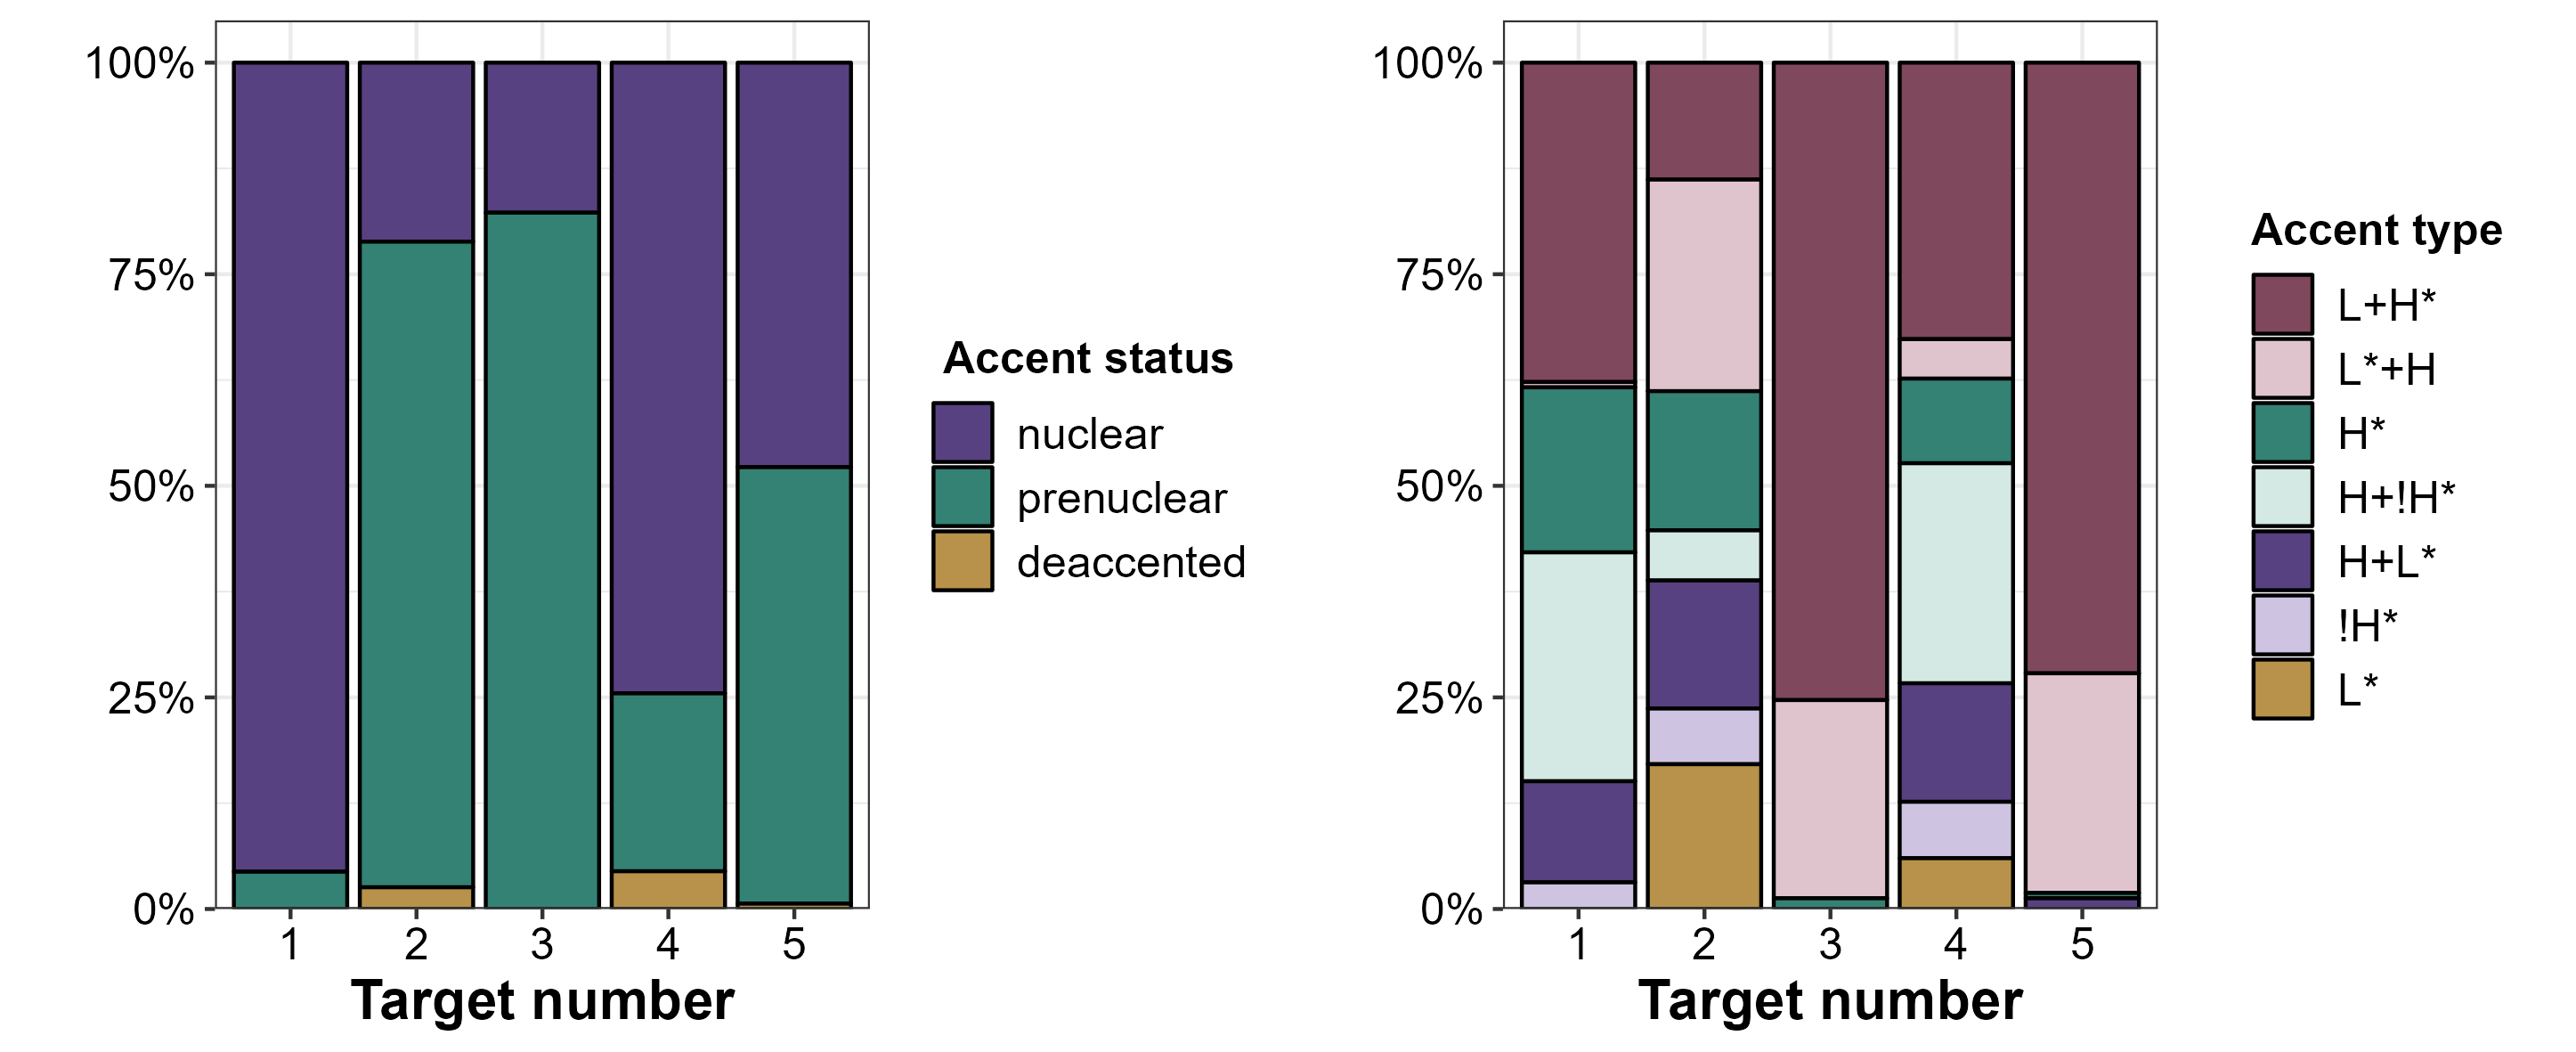
\includegraphics[scale = 0.5]{s2_accent_statustype}
	\caption{Barplots of the distributions of accent status and accent type by target word position.}
	\label{fig:s2_accent_statustype}
\end{figure}

Turning to the continuous prosodic parameters, Figure \ref{fig:s2_cont_parameters} shows the means and standard deviations for each of the eight z-scored prosodic parameters by target word condition. The top panels show the F0-related parameters F0 at CoM, Delta F0, CoG, and synchrony. Average F0 at CoM and Delta F0 values are highest in Targets 3, 5, and 1 and lowest in Target 2, which reflects the accent type distributions reported in the previous paragraph. Similarly, synchrony is on average highest in the initial target words (3 and 5) and is associated with relatively small standard deviations, which is in line with the observation that these words are almost exclusively produced with rising accents. CoG is later aligned in Targets 2 and 3 and earlier in Targets 4 and 5.\footnote{The variability in CoG between the different target word conditions can partially be explained by the different accent types associated with these conditions: Target 4 is produced with more falling accents (characterized by an early CoG) and fewer late rising L*+H accents (characterized by a late CoG) than Target 2 yielding overall earlier CoG alignment in Target 4. However, Target 3 and Target 5 are produced with very similar accent types, yet still differ in CoG alignment. This indicates that CoG as a phonetic parameter is still modified within any category boundaries of different accent types.} The parameters related to timing and intensity on average exhibit the highest values for Target 5, followed by Targets 3 and 1. Target 2 is produced with the lowest intensity and periodic energy mass values, while both Targets 2 and 4 exhibit the shortest average durations.

\begin{figure}
		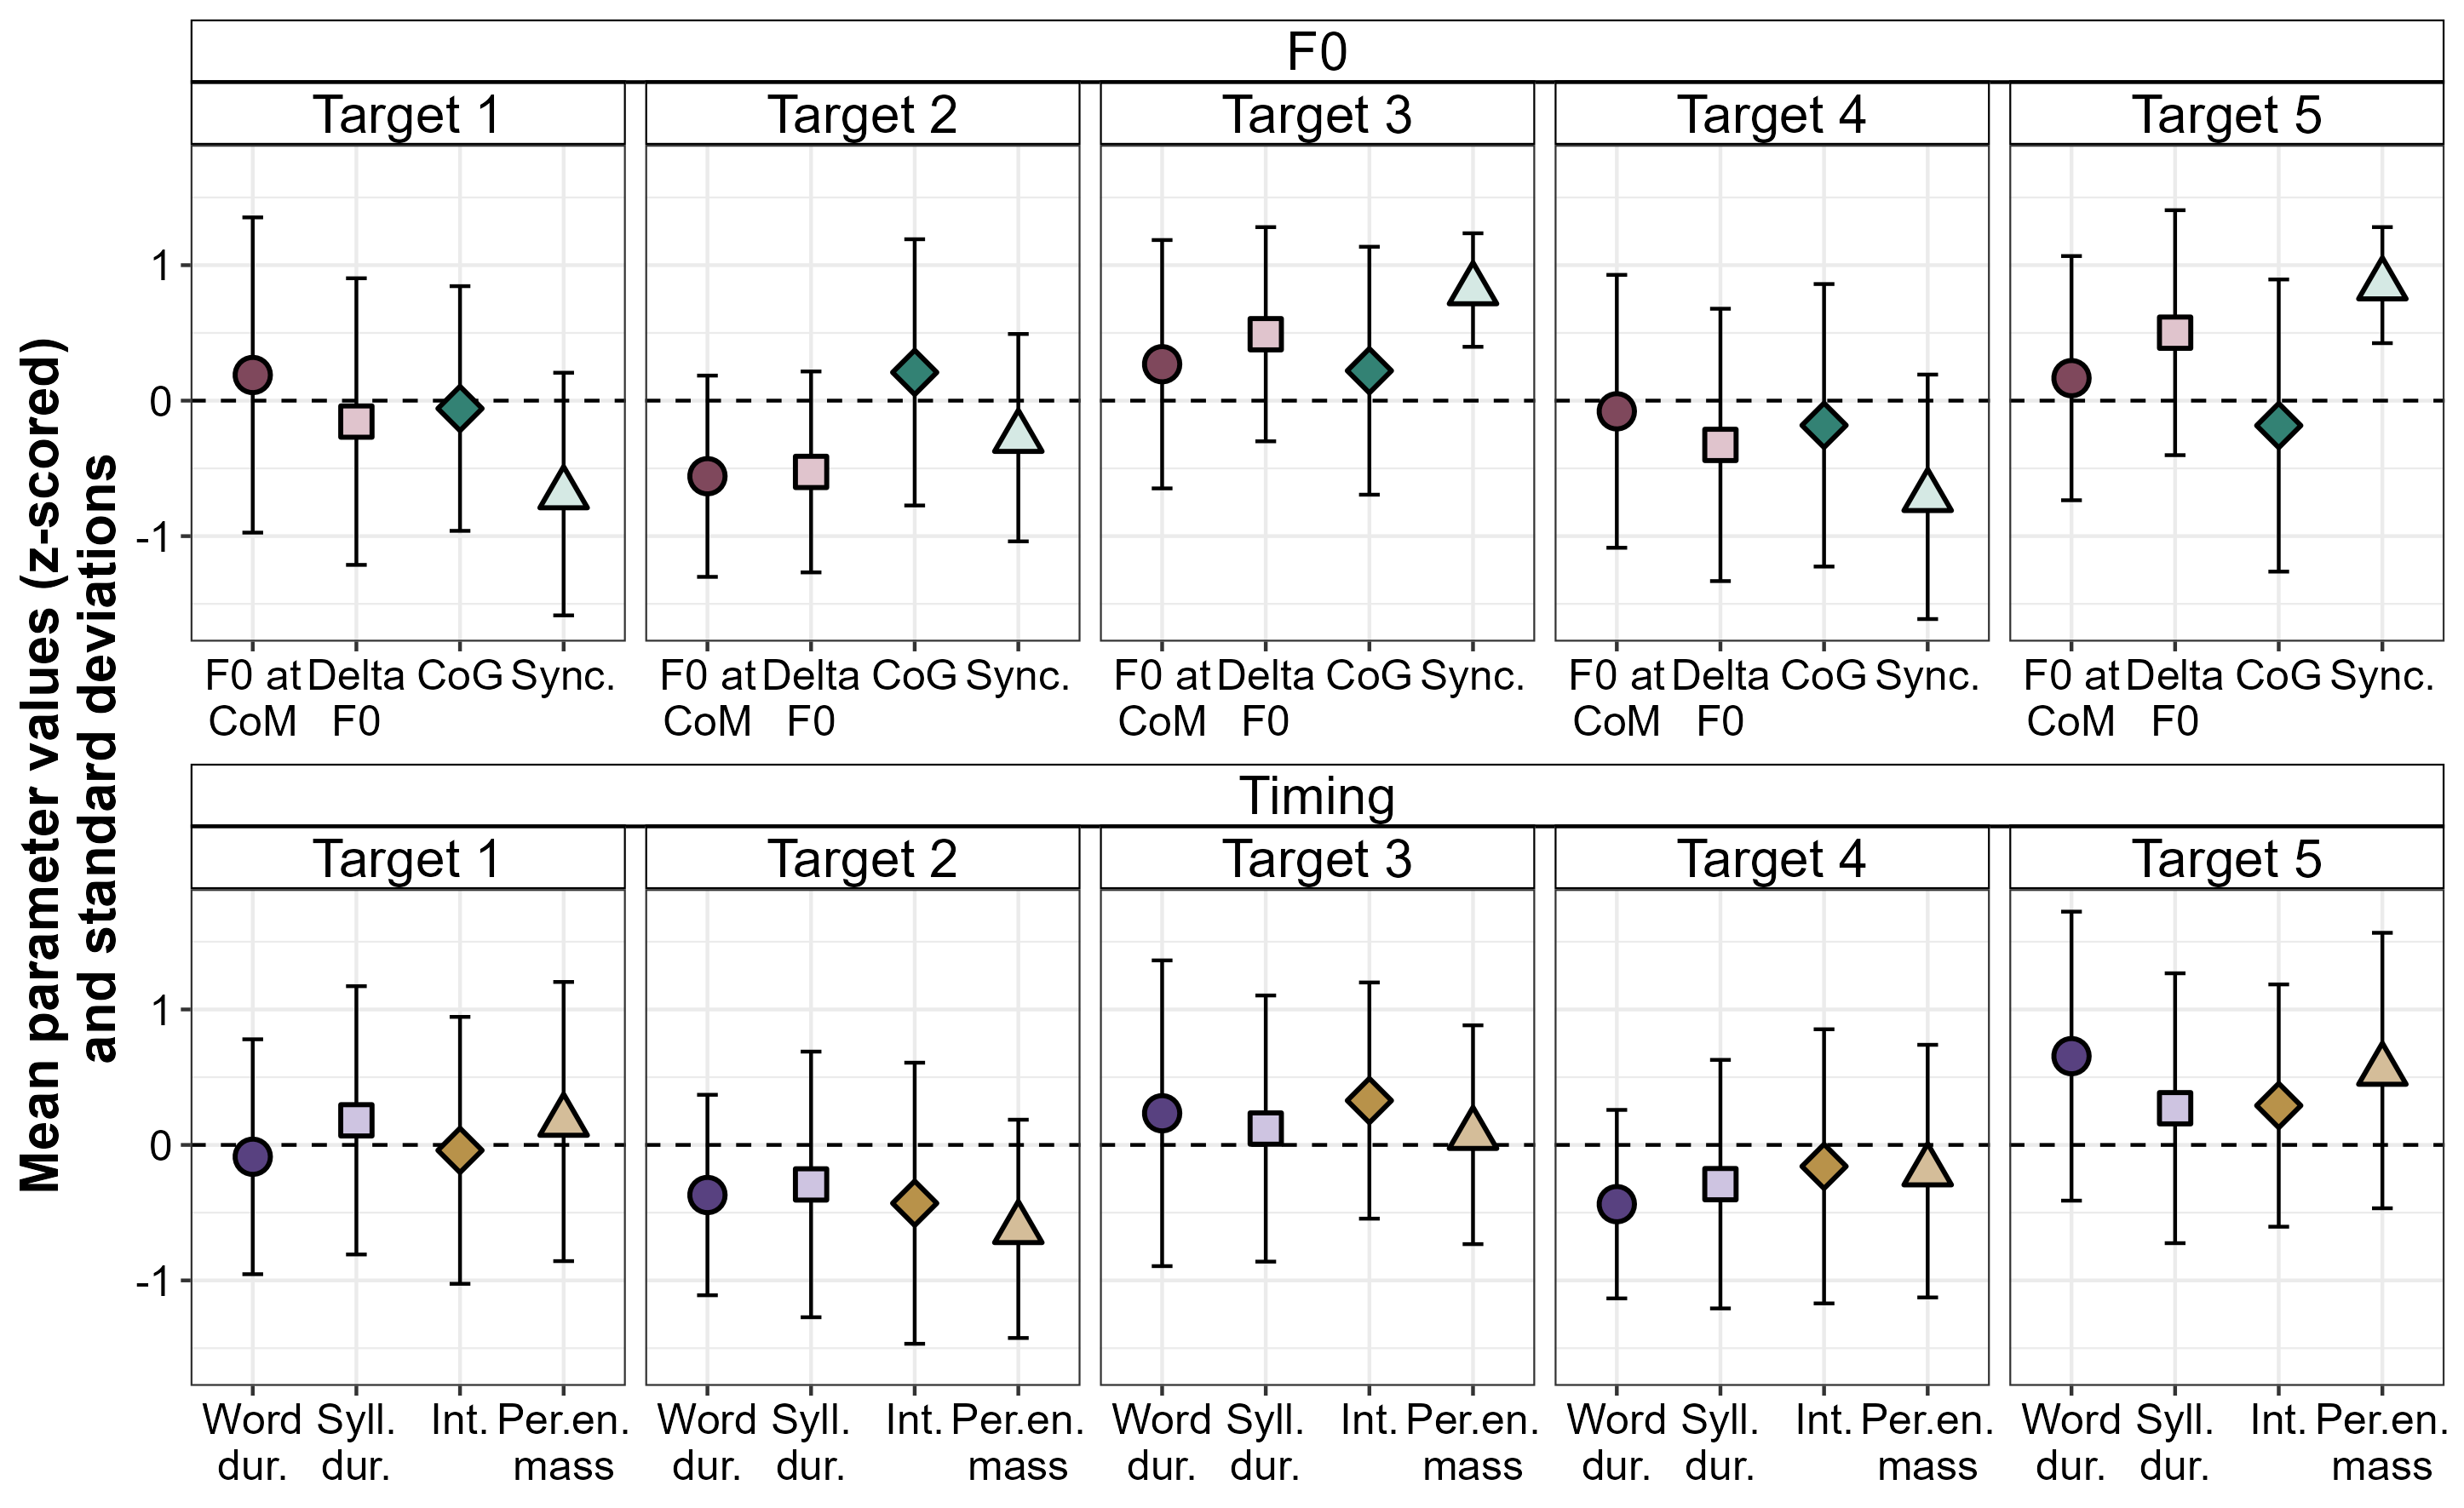
\includegraphics[scale = 0.5]{s2_cont_parameters}
	\caption{Means and standard deviations of all continuous prosodic parameters (z-scored) by target word position. Top panels: Parameters describing the F0 contour. Bottom panels: Parameters related to timing.}
	\label{fig:s2_cont_parameters}
\end{figure}

To disentangle the effects of the manipulated factors on the trends observed in the raw data, we turn to the results of the Bayesian regression models. For lexical givenness, we observe consistent albeit not reliable (following the criteria for reliability specified in Section \ref{sec:Production2 statistics}) effects of accent status and accent type, which are summarized in Table \ref{table:model_parameterscat_lexical_givenness}. Lexically new target words are more likely to be produced with nuclear accents rather than with prenuclear accents or deaccented compared to lexically given target words. They also receive more prominent accent types, although this trend is weaker.

\begin{table}[]
\begin{tabular}{lrrr}
\lsptoprule
\multicolumn{4}{c}{Lexical givenness} \\ \hline
Variable    & $\beta$ & 90\% CrI  & Pr($\beta$\textgreater{}0) \\ \hline
Accent status    & 1.36       & {[}-0.37; 2.91{]}  & 0.91                          \\
Accent type        & 0.38       & {[}-0.31; 1.03{]} & 0.83                          \\
\lspbottomrule
\end{tabular}
\caption{Model parameters describing the effects of lexical givenness on accent status and accent type.}
\label{table:model_parameterscat_lexical_givenness}
\end{table}

Table \ref{table:model_parameters_lexical_givenness} summarizes the model parameters describing the effects of lexical givenness on the continuous prosodic cues. On average, l-new referents are produced with higher values in seven out of the eight prosodic parameters than l-given referents. The strongest, most reliable effects are observed for word duration, syllable duration, and periodic energy mass (Pr($\beta$\textgreater{}0)\textgreater{}0.95), l-new referents being produced with longer duration of the target word and its stressed syllable and higher periodic energy mass in the stressed syllable than l-given referents. There is also strong evidence that l-new referents are produced with higher F0 at CoM and higher intensity in the stressed syllable relative to l-given referents. Furthermore, l-new referents appear to exhibit higher Delta F0 and a later CoG, however, evidence to support these tendencies is much weaker. Finally, synchrony does not appear to vary systematically between l-new and l-given referents with a $\beta$ estimate close to 0.

\begin{table}[]
\begin{tabular}{lrrr}
\lsptoprule
\multicolumn{4}{c}{Lexical givenness} \\ \hline
Variable    & $\beta$ & 90\% CrI  & Pr($\beta$\textgreater{}0) \\ \hline
F0 at CoM    & 0.19       & {[}0.00; 0.38{]}  & 0.95                          \\
Delta F0    & 0.09       & {[}-0.15; 0.34{]}  & 0.75                          \\
Center of Gravity            & 0.09       & {[}-0.14; 0.31{]}  & 0.76                          \\
Synchrony            & -0.02       & {[}-0.28; 0.25{]}  & 0.45                          \\
Word duration            & 0.31       & {[}0.09; 0.53{]}  & 0.99                          \\
Syllable duration & 0.43       & {[}0.20; 0.65{]}  & 1.00                             \\
Intensity             & 0.13       & {[}0.00; 0.26{]} & 0.95                          \\
Periodic energy mass         & 0.36       & {[}0.18; 0.52{]} & 1.00                          \\
\lspbottomrule
\end{tabular}
\caption{Model parameters describing the effects of lexical givenness on the continuous prosodic parameters.}
\label{table:model_parameters_lexical_givenness}
\end{table}

Referential givenness influences accent status in the expected direction, i.e., r-new target words are more likely produced with nuclear accents than r-given target words, although this effect is not reliable (see Table \ref{table:model_parameterscat_referential_givenness}). Accent type does not appear to systematically encode referential givenness.

\begin{table}[]
\begin{tabular}{lrrr}
\lsptoprule
\multicolumn{4}{c}{Referential givenness} \\ \hline
Variable    & $\beta$ & 90\% CrI  & Pr($\beta$\textgreater{}0) \\ \hline
Accent status    & 1.33       & {[}-0.25; 2.78{]}  & 0.92                         \\
Accent type        & 0.13       & {[}-0.71; 0.92{]} & 0.61                          \\
\lspbottomrule
\end{tabular}
\caption{Model parameters describing the effects of referential givenness on accent status and accent type.}
\label{table:model_parameterscat_referential_givenness}
\end{table}

Table \ref{table:model_parameters_referential_givenness} summarizes the model parameters describing the effects of referential givenness on the continuous prosodic cues. R-new referents are reliably marked by a higher F0 at CoM, higher intensity, and higher periodic energy mass of the stressed syllable (Pr($\beta$\textgreater{}0)\textgreater{}0.95) compared to r-given referents. In addition, there is some evidence for a higher Delta F0 in r-new referents. Contrary to expectations, there is reliable evidence that r-new referents are produced with an earlier CoG and lower synchrony than r-given referents (Pr($\beta$\textgreater{}0)\textless{}0.05), indicating an earlier alignment of the F0 peak. While it appears that word duration tends to be longer in r-given referents, syllable duration does not encode referential givenness with a posterior distribution centered around 0.

\begin{table}[]
\begin{tabular}{lrrr}
\lsptoprule
\multicolumn{4}{c}{Referential givenness} \\ \hline
Variable    & $\beta$ & 90\% CrI  & Pr($\beta$\textgreater{}0) \\ \hline
F0 at CoM    & 0.45       & {[}0.20; 0.69{]}  & 1.00                          \\
Delta F0    & 0.18       & {[}-0.10; 0.46{]}  & 0.86                          \\
Center of Gravity            & -0.37       & {[}-0.62; -0.12{]}  & 0.01                          \\
Synchrony            & -0.43       & {[}-0.81; -0.05{]}  & 0.03                          \\
Word duration            & -0.06       & {[}-0.19; 0.07{]}  & 0.21                          \\
Syllable duration & 0.00       & {[}-0.23; 0.22{]}  & 0.50                             \\
Intensity             & 0.26       & {[}0.12; 0.39{]} & 1.00                          \\
Periodic energy mass         & 0.41       & {[}0.23; 0.59{]} & 1.00                          \\
\lspbottomrule
\end{tabular}
\caption{Model parameters describing the effects of referential givenness on the continuous prosodic parameters.}
\label{table:model_parameters_referential_givenness}
\end{table}

For grammatical role, there is a reliable effect on accent status in that objects are more likely to occupy stronger metrical positions than subjects (see Table \ref{table:model_parameterscat_gramm_role}). However, the effect of grammatical role on accent type is reversed, with subjects receiving more prominent accent types than objects, but also somewhat weaker. 

\begin{table}[]
\begin{tabular}{lrrr}
\lsptoprule
\multicolumn{4}{c}{Grammatical role} \\ \hline
Variable    & $\beta$ & 90\% CrI  & Pr($\beta$\textgreater{}0) \\ \hline
Accent status    & 1.33       & {[}0.60; 2.03{]}  & 1.00                          \\
Accent type        & -0.29       & {[}-0.83; 0.25{]} & 0.19                          \\
\lspbottomrule
\end{tabular}
\caption{Model parameters describing the effects of grammatical role on accent status and accent type.}
\label{table:model_parameterscat_gramm_role}
\end{table}

In contrast to lexical and referential givenness, the marking of grammatical role is more subtle in terms of continuous prosodic parameters (see Table \ref{table:model_parameters_gramm_role}). Reliable evidence from the models suggests that objects are produced with an earlier CoG compared to subjects (Pr($\beta$\textgreater{}0)\textless{}0.05). There is also relatively strong evidence that objects are produced with longer syllable duration and higher periodic energy mass than subjects. Weaker evidence suggests that Delta F0, synchrony, and word duration values are higher, while F0 at CoM and intensity of the stressed syllable are lower in objects than in subjects.  

\begin{table}[]
\begin{tabular}{lrrr}
\lsptoprule
\multicolumn{4}{c}{Grammatical role} \\ \hline
Variable    & $\beta$ & 90\% CrI  & Pr($\beta$\textgreater{}0) \\ \hline
F0 at CoM    & -0.09       & {[}-0.22; 0.03{]}  & 0.11                          \\
Delta F0    & 0.04       & {[}-0.11; 0.18{]}  & 0.67                          \\
Center of Gravity            & -0.33       & {[}-0.60; -0.06{]}  & 0.03                          \\
Synchrony            & 0.05       & {[}-0.08; 0.17{]}  & 0.73                          \\
Word duration            & 0.11       & {[}-0.09; 0.31{]}  & 0.82                          \\
Syllable duration & 0.16       & {[}0.00; 0.33{]}  & 0.94                             \\
Intensity             & -0.04       & {[}-0.17; 0.09{]} & 0.30                          \\
Periodic energy mass         & 0.48       & {[}-0.03; 0.95{]} & 0.94                          \\
\lspbottomrule
\end{tabular}
\caption{Model parameters describing the effects of grammatical role on the continuous prosodic parameters.}
\label{table:model_parameters_gramm_role}
\end{table}

Finally, the results for the effect of sentence position on prosody production are very clear, albeit unexpected under the original expectation that words in medial position should be produced with more prosodic prominence than words in initial position. Instead, the initial position is more prominent in terms of both metrical structure (although this effect is not reliable) and accent type choice (see Table \ref{table:model_parameterscat_position}).

\begin{table}[]
\begin{tabular}{lrrr}
\lsptoprule
\multicolumn{4}{c}{Sentence position} \\ \hline
Variable    & $\beta$ & 90\% CrI  & Pr($\beta$\textgreater{}0) \\ \hline
Accent status    & -0.74       & {[}-1.83; 0.44{]}  & 0.14                          \\
Accent type        & -2.80       & {[}-3.78; -1.73{]} & 0.00                          \\
\lspbottomrule
\end{tabular}
\caption{Model parameters describing the effects of sentence position on accent status and accent type.}
\label{table:model_parameterscat_position}
\end{table}

A similar picture emerges for the continuous prosodic parameters. There is reliable evidence that all but one parameter are produced with higher values in an initial than in a medial target word (all Pr($\beta$\textgreater{}0)\textless{}0.05, see Table \ref{table:model_parameters_position}). That is, initial target words are produced with a higher F0 at CoM, higher Delta F0, higher synchrony, longer word and syllable duration, higher intensity, and higher periodic energy mass in the stressed syllable. The one exception is CoG, where there is quite strong evidence that words in medial position are produced with a later CoG than words in initial position. Sentence position thus appears to be the most important factor in modulating prosodic prominence.

\begin{table}[]
\begin{tabular}{lrrr}
\lsptoprule
\multicolumn{4}{c}{Sentence position} \\ \hline
Variable    & $\beta$ & 90\% CrI  & Pr($\beta$\textgreater{}0) \\ \hline
F0 at CoM    & -0.69       & {[}-1.00; -0.36{]}  & 0.00                          \\
Delta F0    & -0.96       & {[}-1.28; -0.63{]}  & 0.00                          \\
Center of Gravity            & 0.35       & {[}-0.04; 0.72{]}  & 0.94                          \\
Synchrony            & -1.10       & {[}-1.38; -0.82{]}  & 0.00                          \\
Word duration            & -0.51       & {[}-0.73; -0.30{]}  & 0.00                          \\
Syllable duration & -0.52       & {[}-0.83; -0.20{]}  & 0.01                             \\
Intensity             & -0.71       & {[}-0.90; -0.52{]} & 0.00                          \\
Periodic energy mass         & -1.23       & {[}-1.62; -0.80{]} & 0.00                          \\
\lspbottomrule
\end{tabular}
\caption{Model parameters describing the effects of sentence position on the continuous prosodic parameters.}
\label{table:model_parameters_position}
\end{table}

\subsection{Individual strategies}

After establishing a baseline of the overall effects across speakers, this section explores individual differences and similarities in the prosodic encoding of lexical and referential givenness, grammatical role, and sentence position. As in the previous study (see Chapter \ref{ch:Production I}), we first take a descriptive approach to individual variability. Figure \ref{fig:s2_accent_status_byspeaker} illustrates the distribution of accent status across the five target word conditions for each speaker. Most obviously, only five out of 20 speakers use deaccentuation at all. A similarity is that for all speakers except one (s16), Target 1 is the most likely to be produced with a nuclear accent, i.e., the most prominent, and in fact, 16 speakers produce Target 1 exclusively with a nuclear accent. For most speakers (n = 16), Target 4 is the second most likely to receive a nuclear accent or equally as likely as Target 1. There are three speakers who produce Target 5 more prominently than Target 4, namely, s05, s09, and s20. Looking at only the medial target words (1, 2, and 4), Target 2 is consistently the least prominent of the three for every speaker, as it is produced with at most 50\% nuclear accents (s03, s13) but more often with exclusively prenuclear accents (s07, s09, s11, s17). There is more variability with regard to the initial target words (3 and 5). Some speakers produce only prenuclear accents in both positions (s04, s07, s14, s16) but one speaker (s09) produces only nuclear accents on Target 5. In most speakers (n = 14), Target 5 is more likely to receive a nuclear accent than Target 3. 

\begin{figure}
		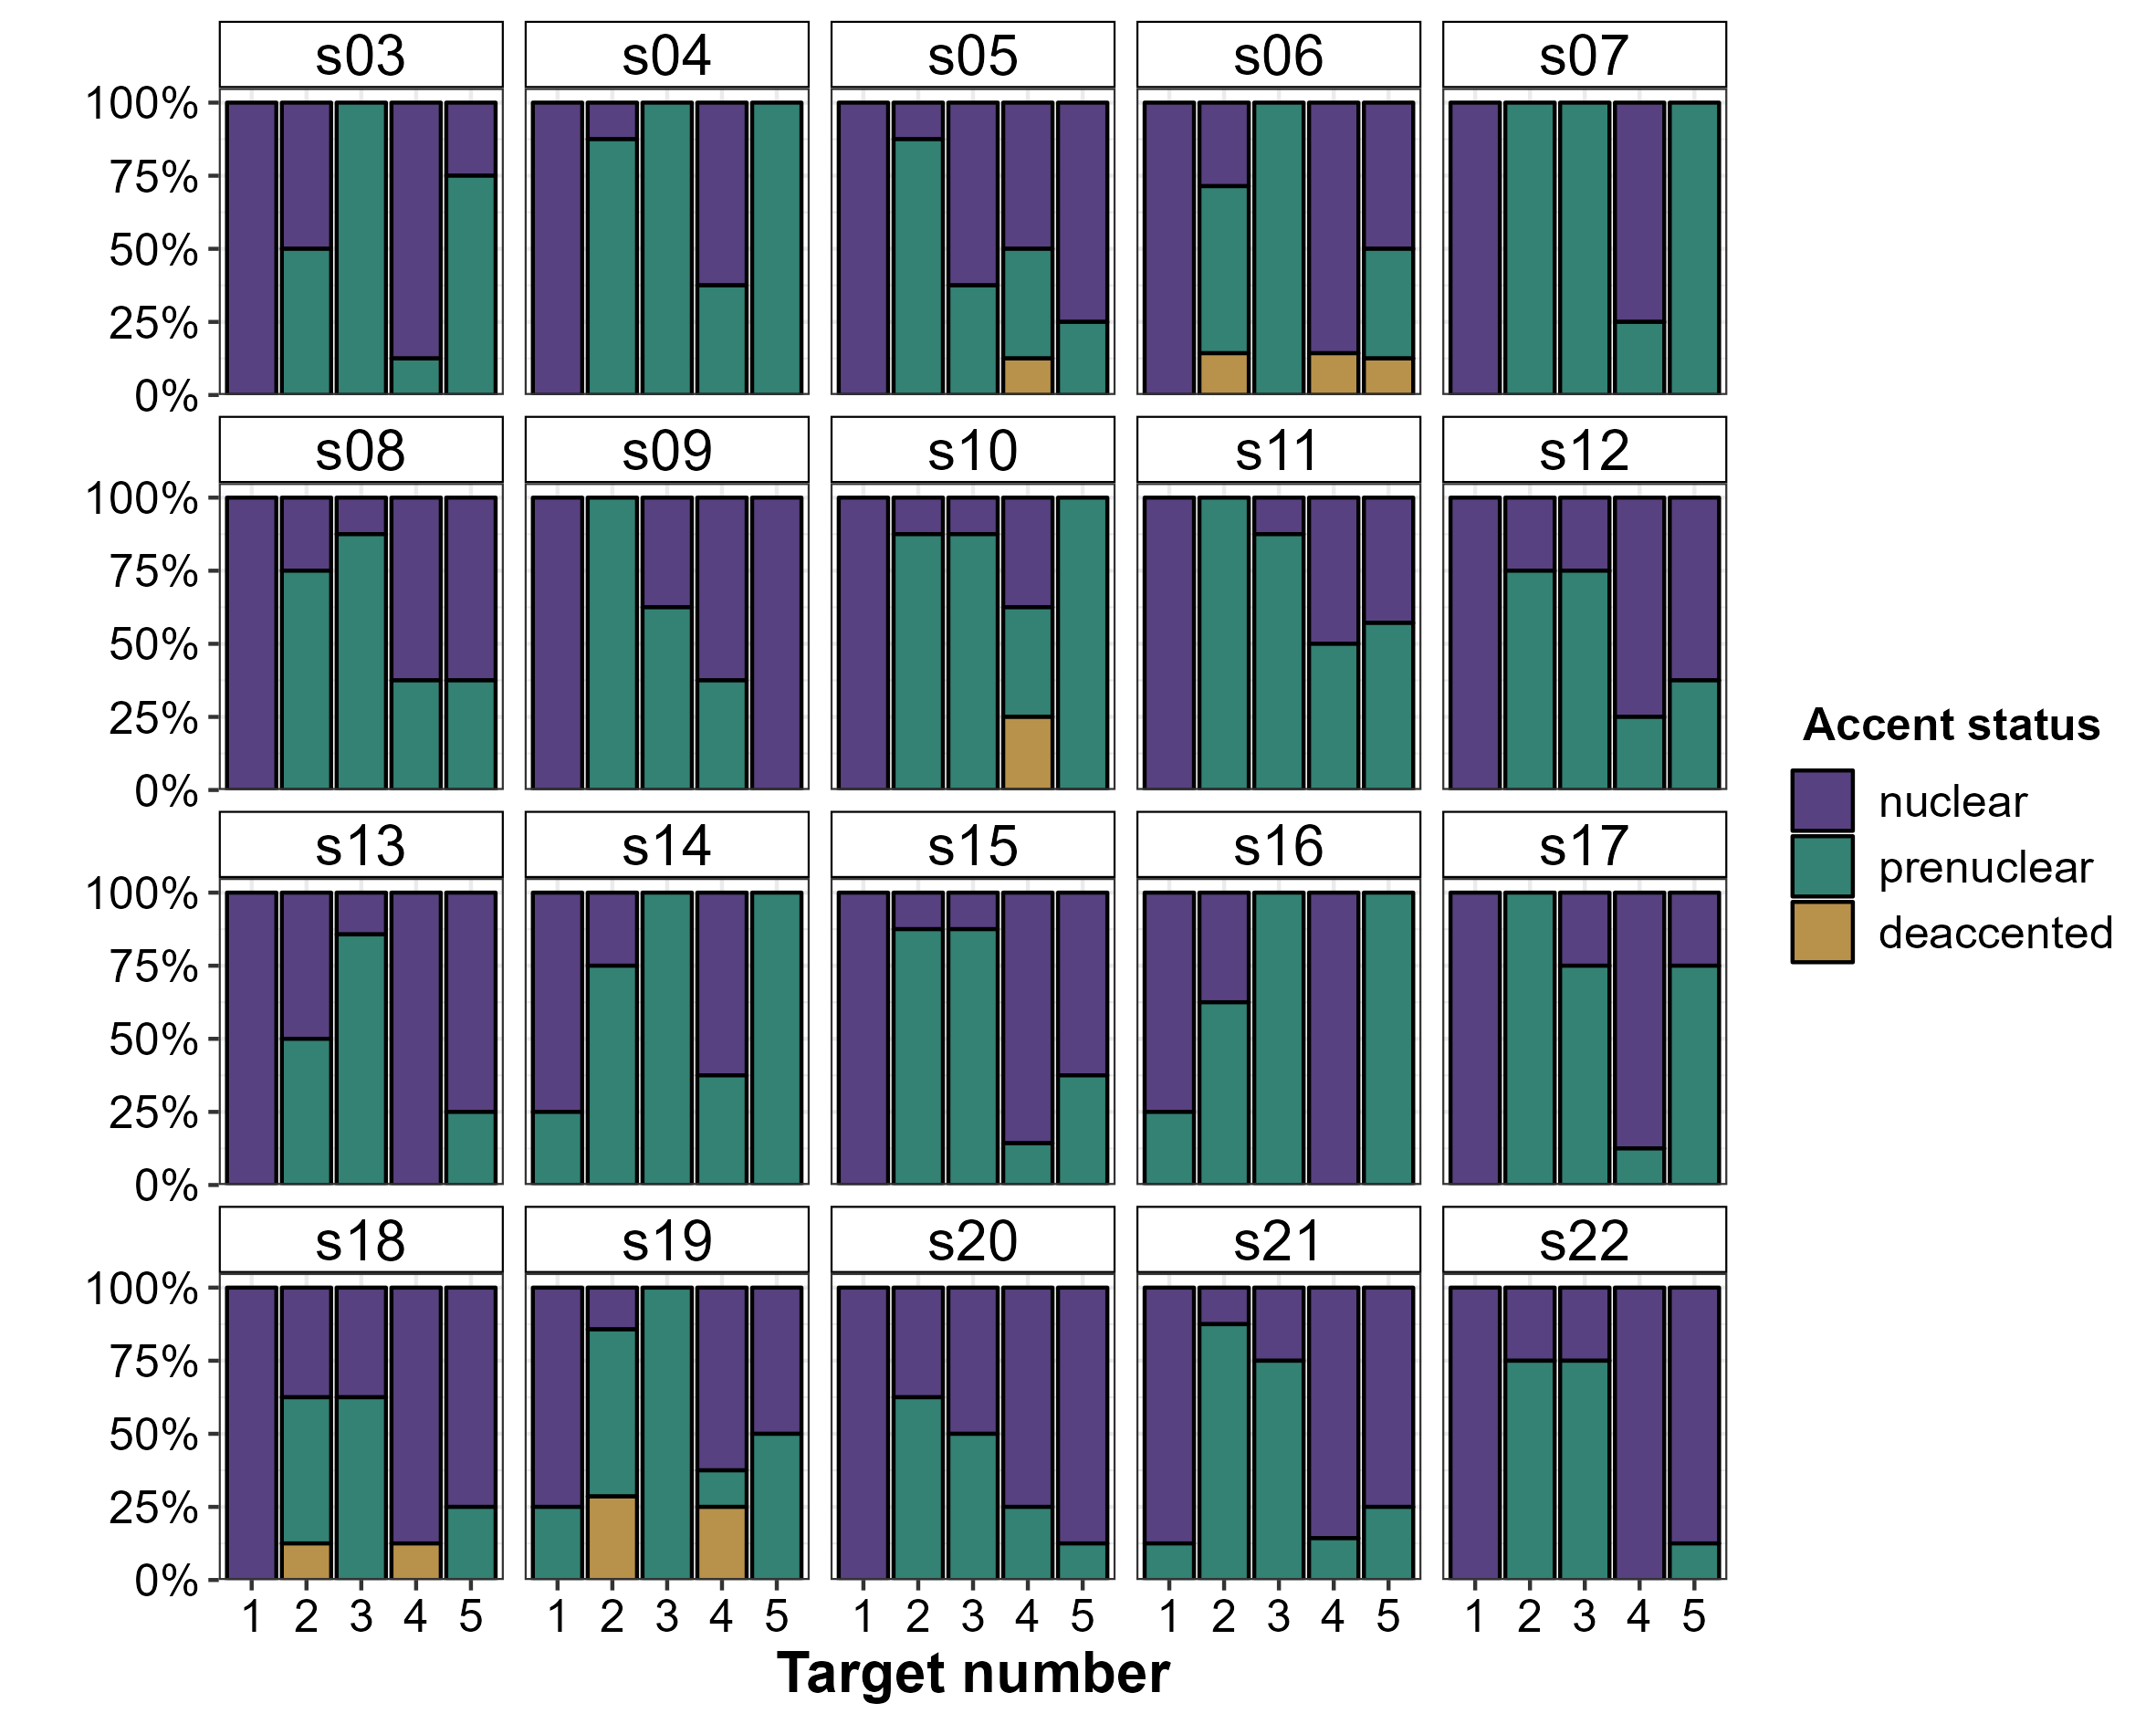
\includegraphics[width=\textwidth]{s2_accent_status_byspeaker}
	\caption{Distributions of accent status across target word positions per speaker.}
	\label{fig:s2_accent_status_byspeaker}
\end{figure}

Next, we look at the usage of pitch accent types across the target word conditions (see Figure \ref{fig:s2_accent_type_byspeaker}). There is generally more variability in terms of accent types used in the medial target words (1, 2, and 4) than the initial ones (3 and 5) and initial target words are produced consistently with more prominent accent types across speakers, which is in line with the averaged result in Section \ref{sec:Production2 overall results} above. In fact, ten speakers produce only L*+H and L+H* accents on initial target words and another six speakers produce exclusively L+H* accents on Targets 3 and 5. In contrast to the prominence ranking observed for Targets 3 and 5 in terms of accent status, the accent type distributions do not yield such clear results. Specifically, there are only four speakers (s05, s12, s13, and s17) who use more prominent accent types on Target 5 than Target 3, but seven speakers (s04, s06, s09, s14, s15, s20, s22) who use more prominent accent types on Target 3. In the medial target words (1, 2, and 4), speakers typically use between two and five different accent types per condition. Due to this diversity, it is much harder to detect systematic patterns by visually inspecting the plots. Nevertheless, half of the speakers (s06, s07, s08, s11, s12, s13, s15, s19, s20, and s21) use more L+H* (i.e., the most prominent accent type) in  Target 1 than in Targets 2 and 4, which is in the anticipated direction. In addition, Target 2, which was expected to be the least prominent of the medial target words, is realized with a larger proportion of the least prominent L* accent than Targets 1 and 4 by eight speakers (s04, s07, s09, s12, s13, s17, s19, s21). However, the prominence ranking between  Targets 1 and 4 in terms of accent type is not at all clear. Focusing on just the proportions of L+H*, only six speakers exhibit the expected ranking of 1 > 4 > 2 (s07, s08, s15, s19, s20, s21). In contrast, eight speakers produce their highest proportions of L+H* (in medial target words) in Target 2 (s05, s17) or Target 4 (s04, s09, s10, s16, s18, s22). This reflects the inconclusive overall results concerning accent type presented in Section \ref{sec:Production2 overall results}, especially regarding the effects of referential givenness. 

\begin{figure}
		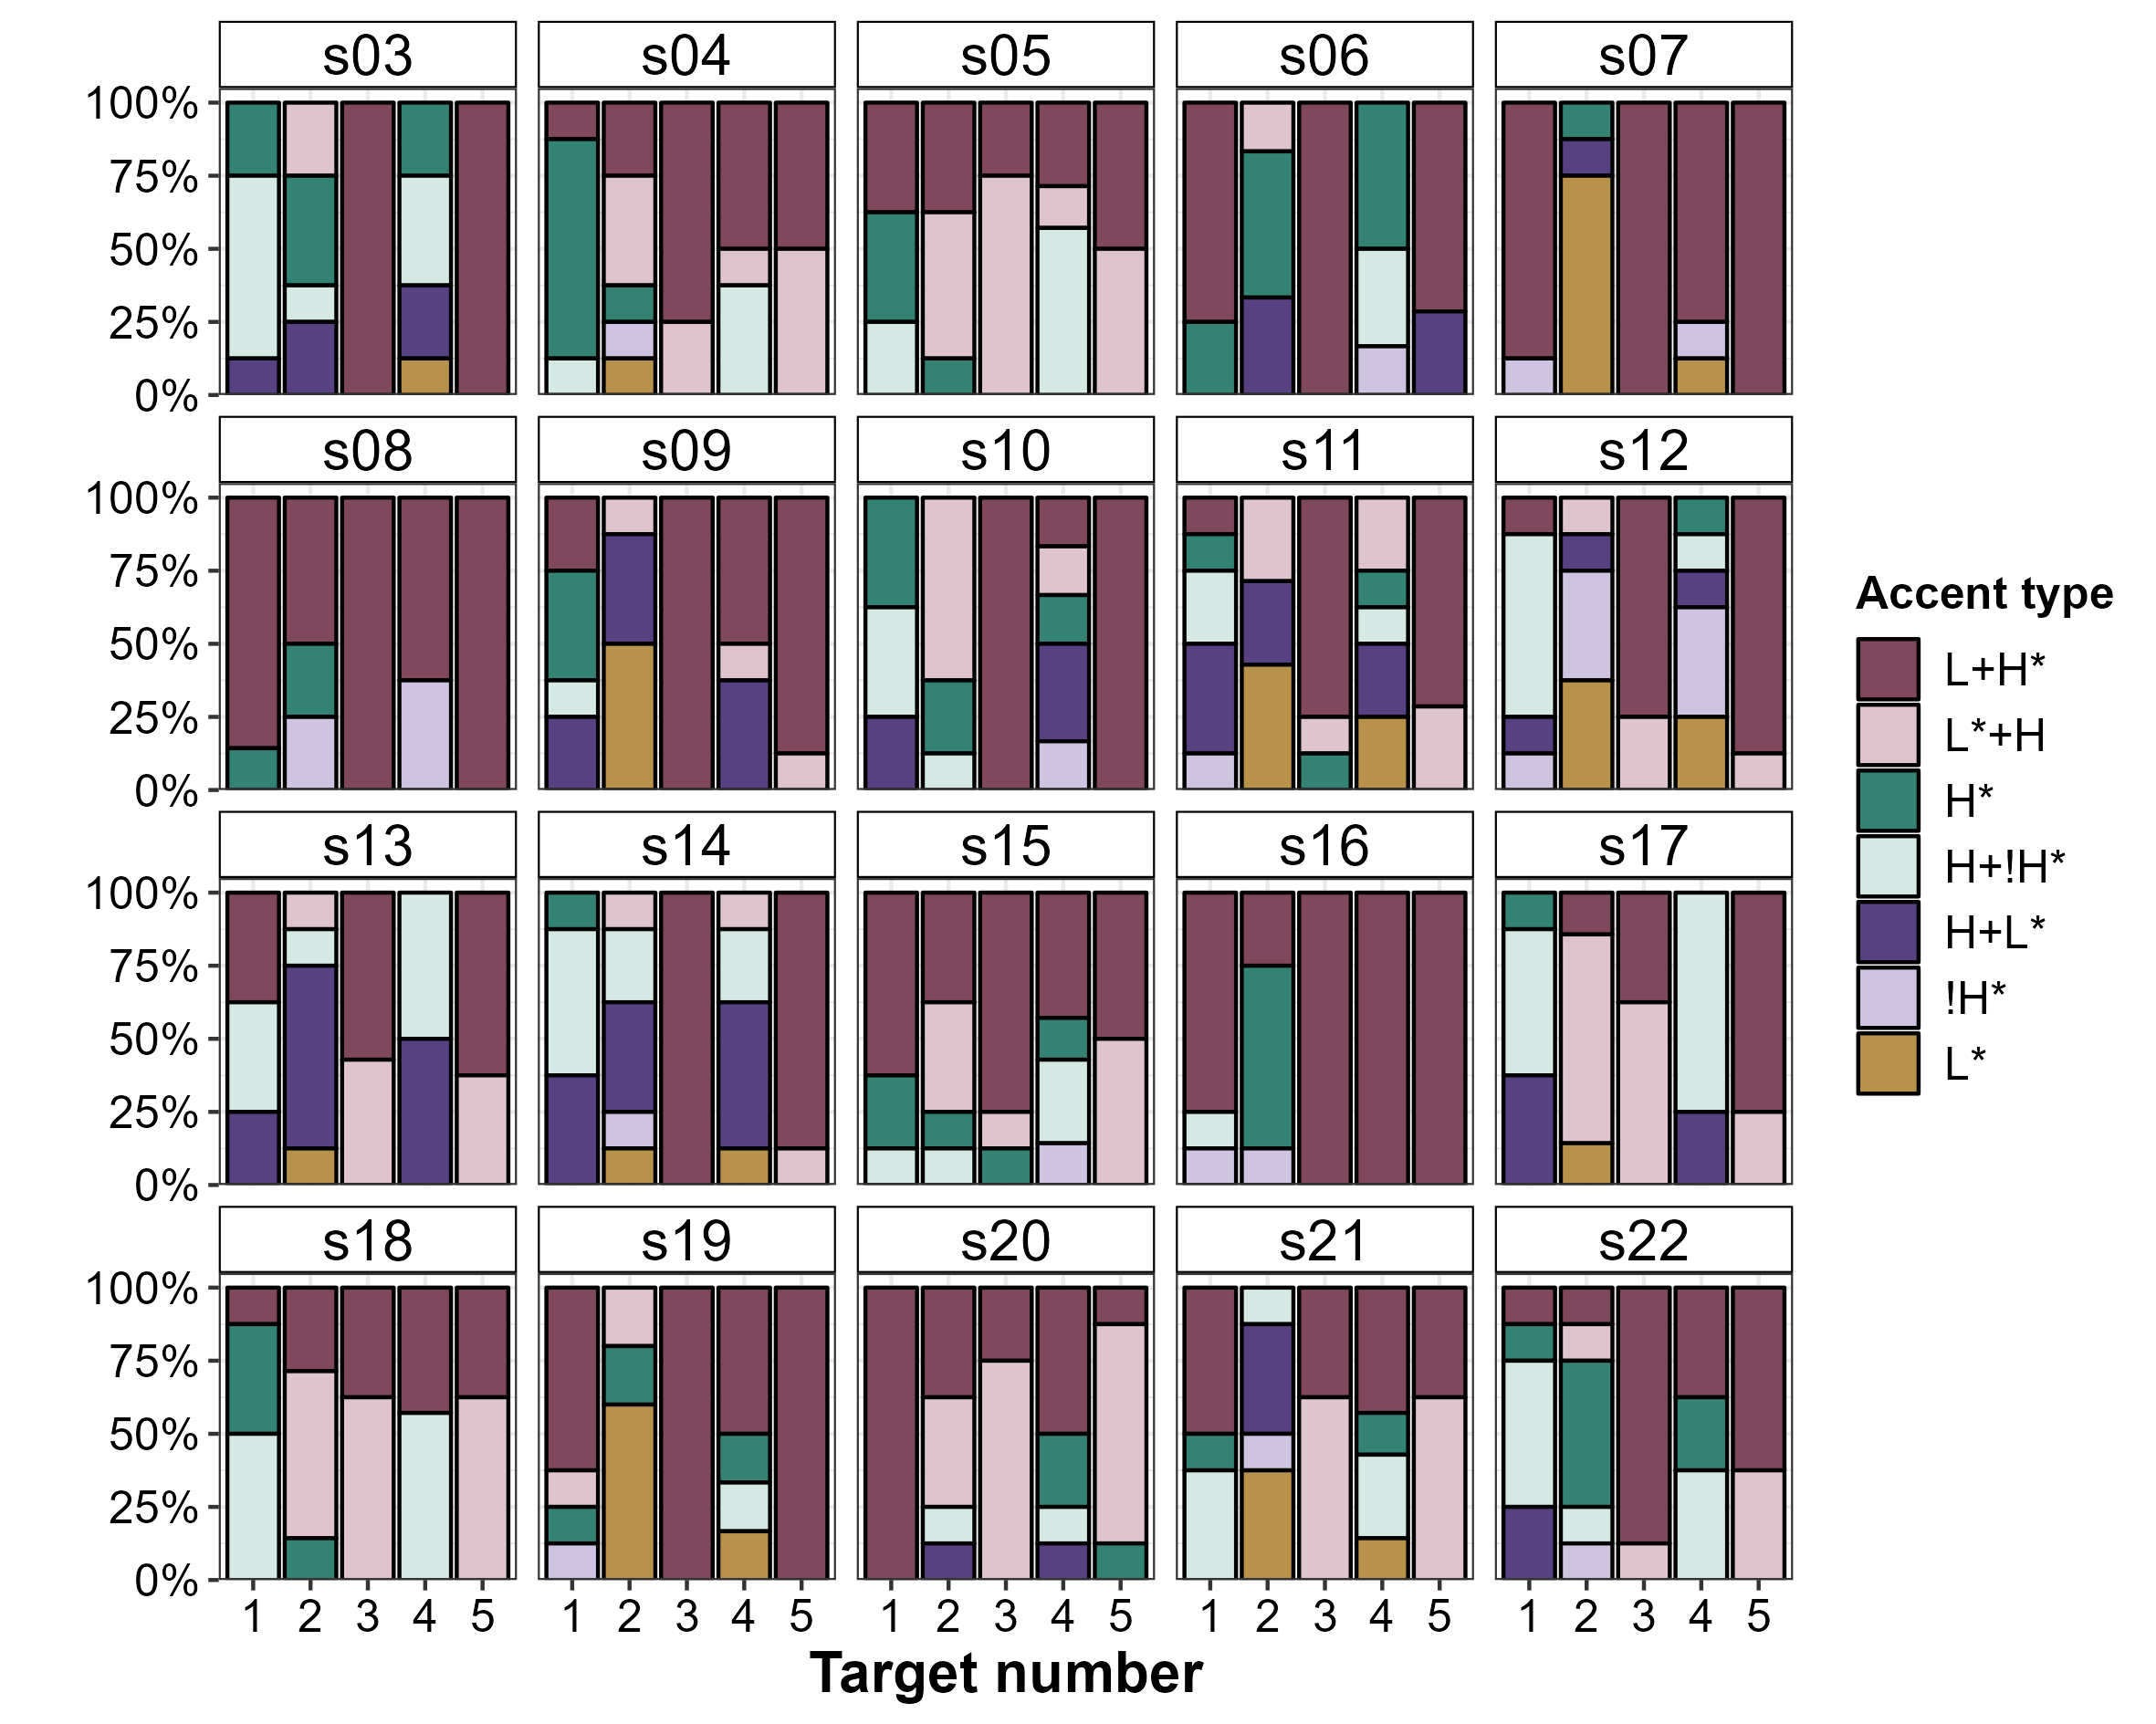
\includegraphics[width=\textwidth]{s2_accent_type_byspeaker}
	\caption{Distributions of pitch accent types across target word positions per speaker.}
	\label{fig:s2_accent_type_byspeaker}
\end{figure}

To more systematically analyze the inter-speaker variability observed in the encoding of the individual semantic-pragmatic and syntactic factors via accent type and accent status, we return to the output of the regression models presented in the previous section. Figure \ref{fig:s2_accentstatus_effects} presents the estimated effect of each of the four factors on accent status per speaker, i.e., the random slope estimates from the accent status model. For lexical givenness, most speakers (18 out of 20) likely produce new target words in such a way that they occupy stronger metrical positions than given words as indicated by the positive mean posterior estimates in Figure \ref{fig:s2_accentstatus_effects} (upper left panel). However, for quite a few speakers, the 90\% CrIs considerably overlap with zero, indicating there is a probability that they exhibit no effect. This is different for referential givenness (Figure \ref{fig:s2_accentstatus_effects}, upper right panel), where 15 speakers clearly show the expected effect of referential givenness on accent status with fully positive 90\% CrIs of the posterior estimates. What is more, mean posterior estimates are positive for all speakers. The number of speakers showing a clearly positive effect of grammatical role on accent status is slightly lower, with 12 speakers producing objects in metrically stronger positions than subjects (Figure \ref{fig:s2_accentstatus_effects}, bottom left panel). Nevertheless, mean estimates are positive throughout all speakers. Finally, for sentence position, seven speakers reliably produce more nuclear accents in the initial position than the medial one (Figure \ref{fig:s2_accentstatus_effects}, bottom right panel). There are also some speakers potentially showing the opposite effect, more prominent accent status in medial target words, although these speakers' 90\% CrIs include zero, indicating the possibility of a null effect. 

\begin{figure}[t]	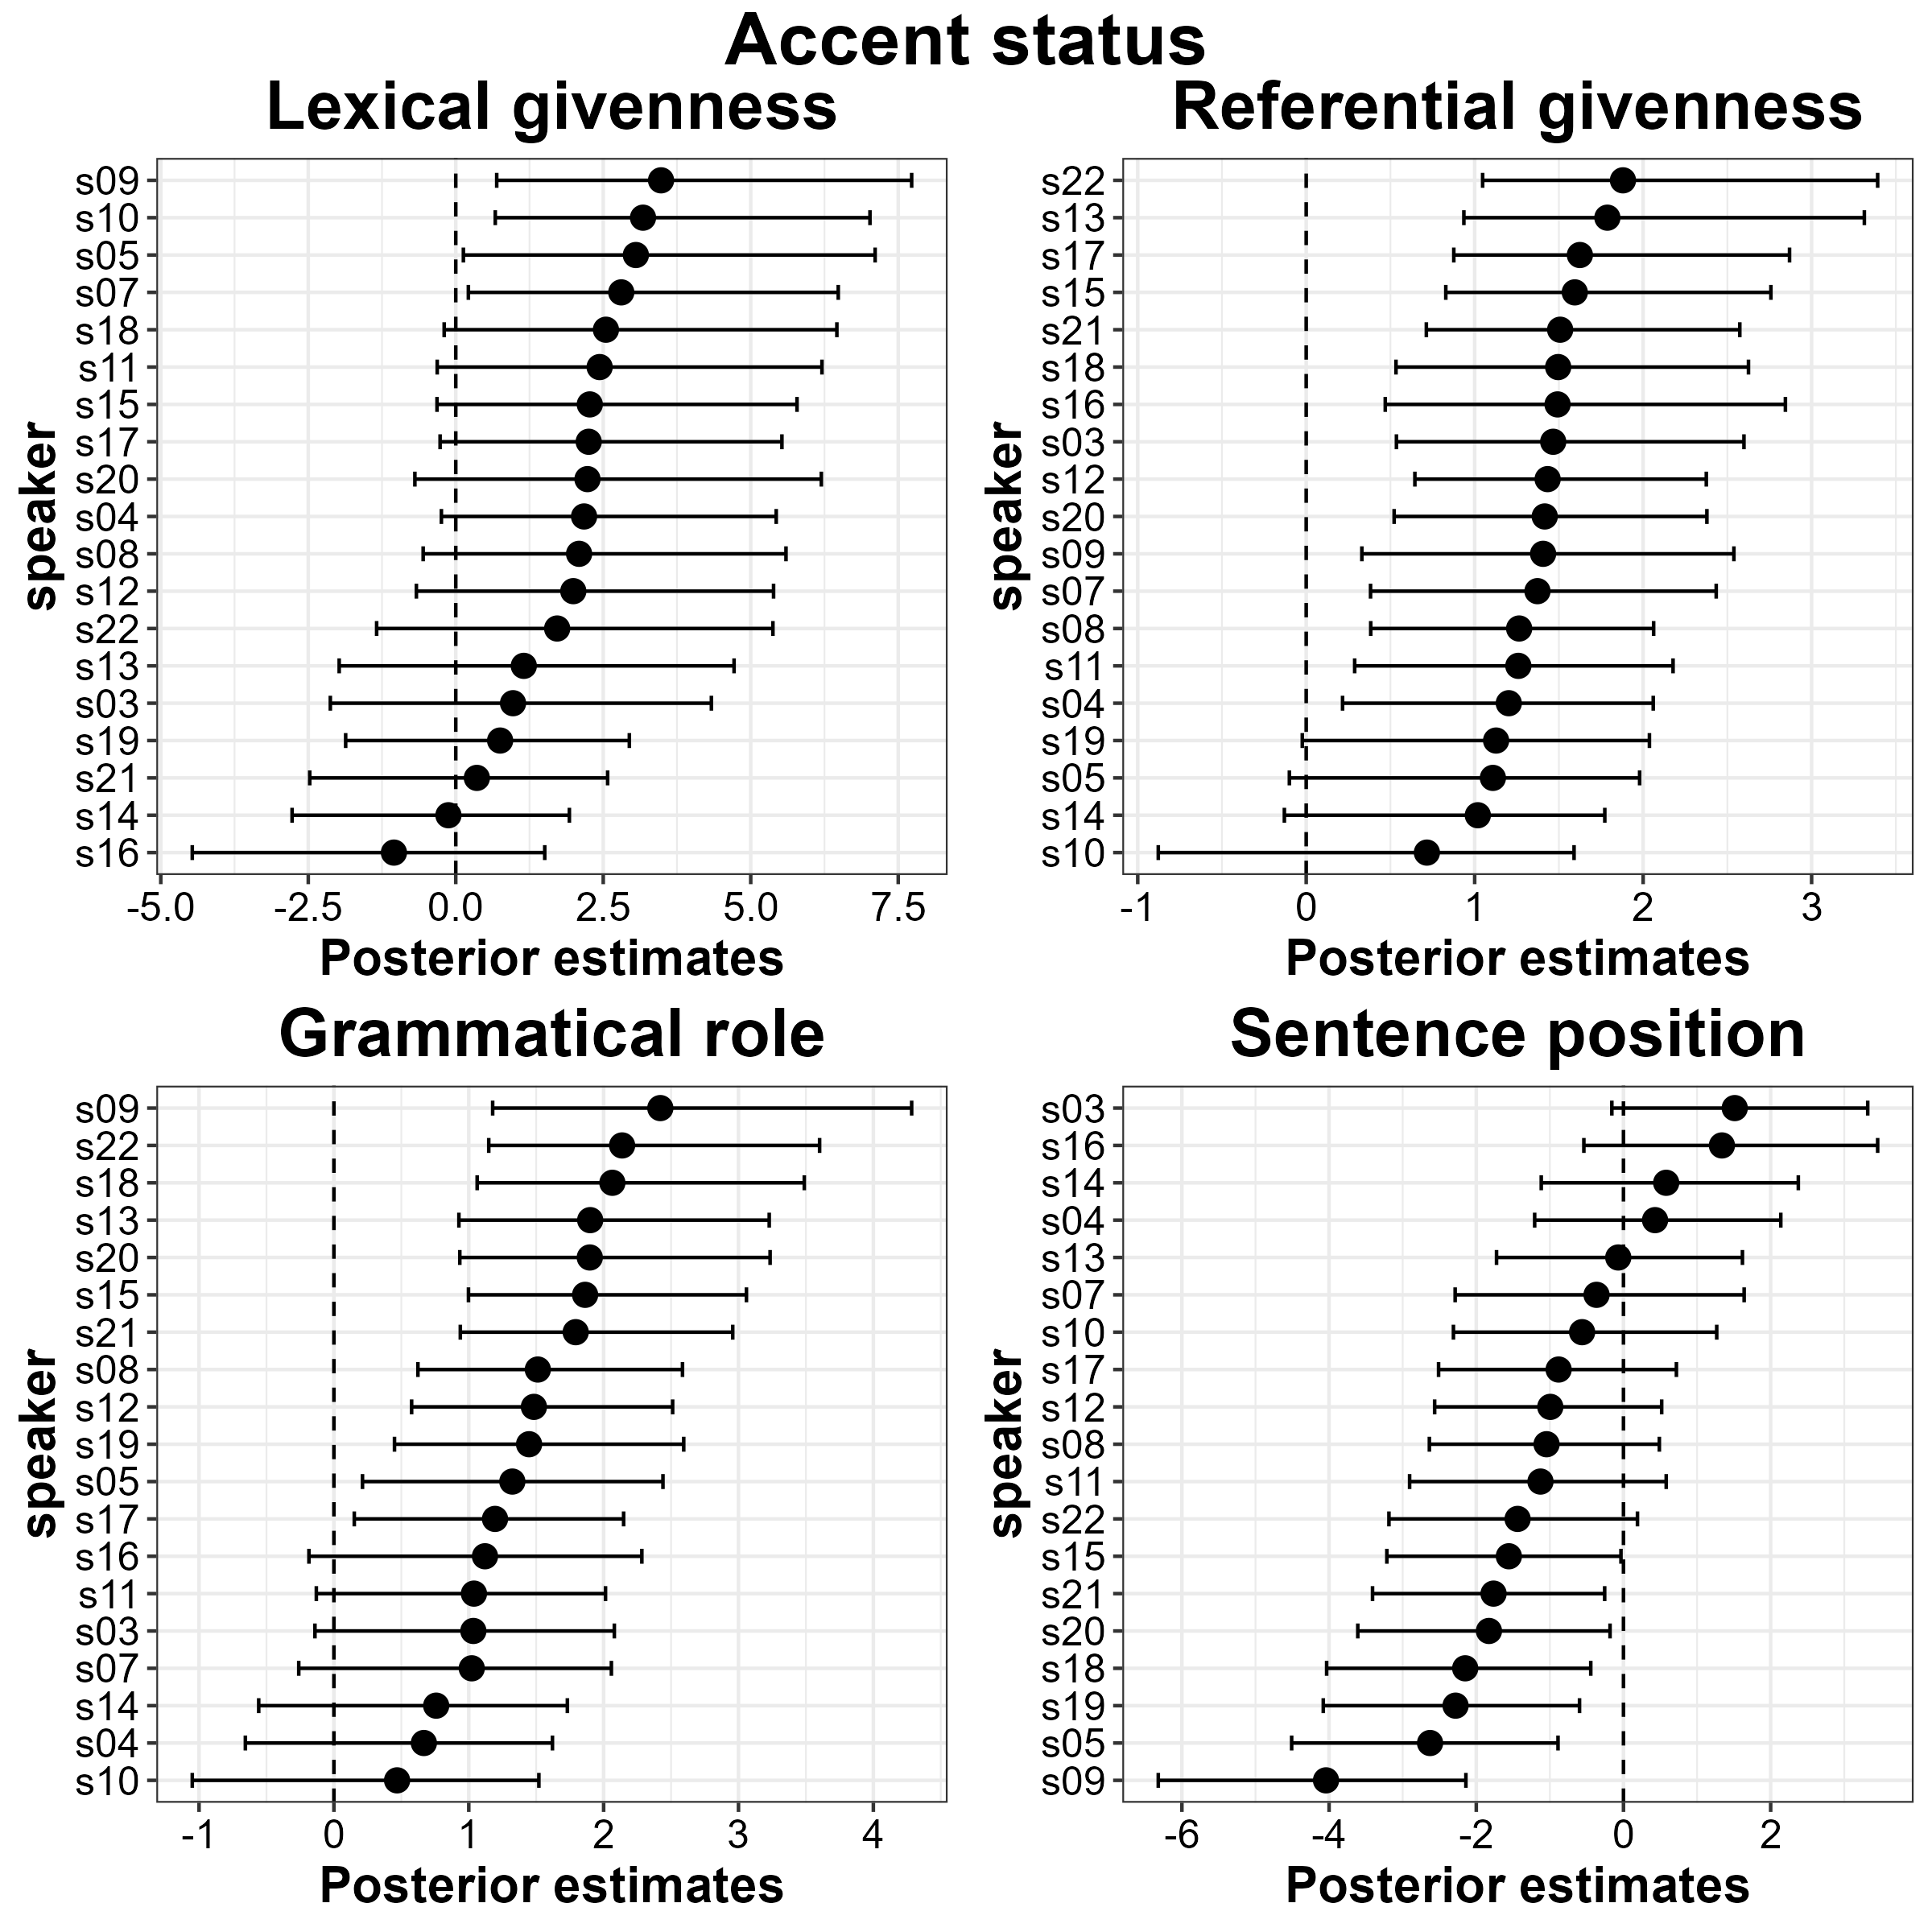
\includegraphics[scale = 0.5]{s2_accentstatus_effects}
	\caption{Means and 90\% CrIs for the effects of lexical and referential givenness, grammatical role, and sentence position on accent status.}
	\label{fig:s2_accentstatus_effects}
\end{figure}

Moving on to the second categorical parameter, accent type, there are two speakers who reliably use more prominent accent types to mark lexical newness (see Figure \ref{fig:s2_accenttype_effects}, upper left panel). In addition, six speakers seem to show relatively strong effects of lexical givenness on accent type. However, the remaining speakers do not seem to make use of this parameter to a reliable extent, with mean posterior estimates close to zero. For referential givenness, there is considerable individual variability in the use of accent type (see Figure \ref{fig:s2_accenttype_effects}, upper right panel). While half of the speakers show a reliable or relatively strong positive effect (i.e., producing more prominent accent types on referentially new entities), three speakers exhibit a reliable effect in the opposite direction, marking referentially given entities with more prominent accent types. Note that the speakers exhibiting the strongest effects of lexical and referential givenness on accent type are not identical to the speakers showing the strongest effects on accent status, i.e. speakers who use accent status to encode either dimension of givenness do not simultaneously make use of accent type to the same end. In fact, speaker s17, who shows one of the strongest positive effects of referential givenness on accent status, produces the strongest negative effect of referential givenness on accent type.

In contrast to the results for referential givenness, there is little variability in the encoding of grammatical role via accent type across speakers (see Figure \ref{fig:s2_accenttype_effects}, bottom left panel). If anything, all speakers have a weak tendency to produce more prominent accent types on subjects than on objects. Finally, there is also little variability in the encoding of sentence position (see Figure \ref{fig:s2_accenttype_effects}, bottom right panel). All speakers exhibit negative effects, i.e., the initial position is associated with more prominent accent types than the medial position. This effect is reliable for 14 speakers. 

\begin{figure}
		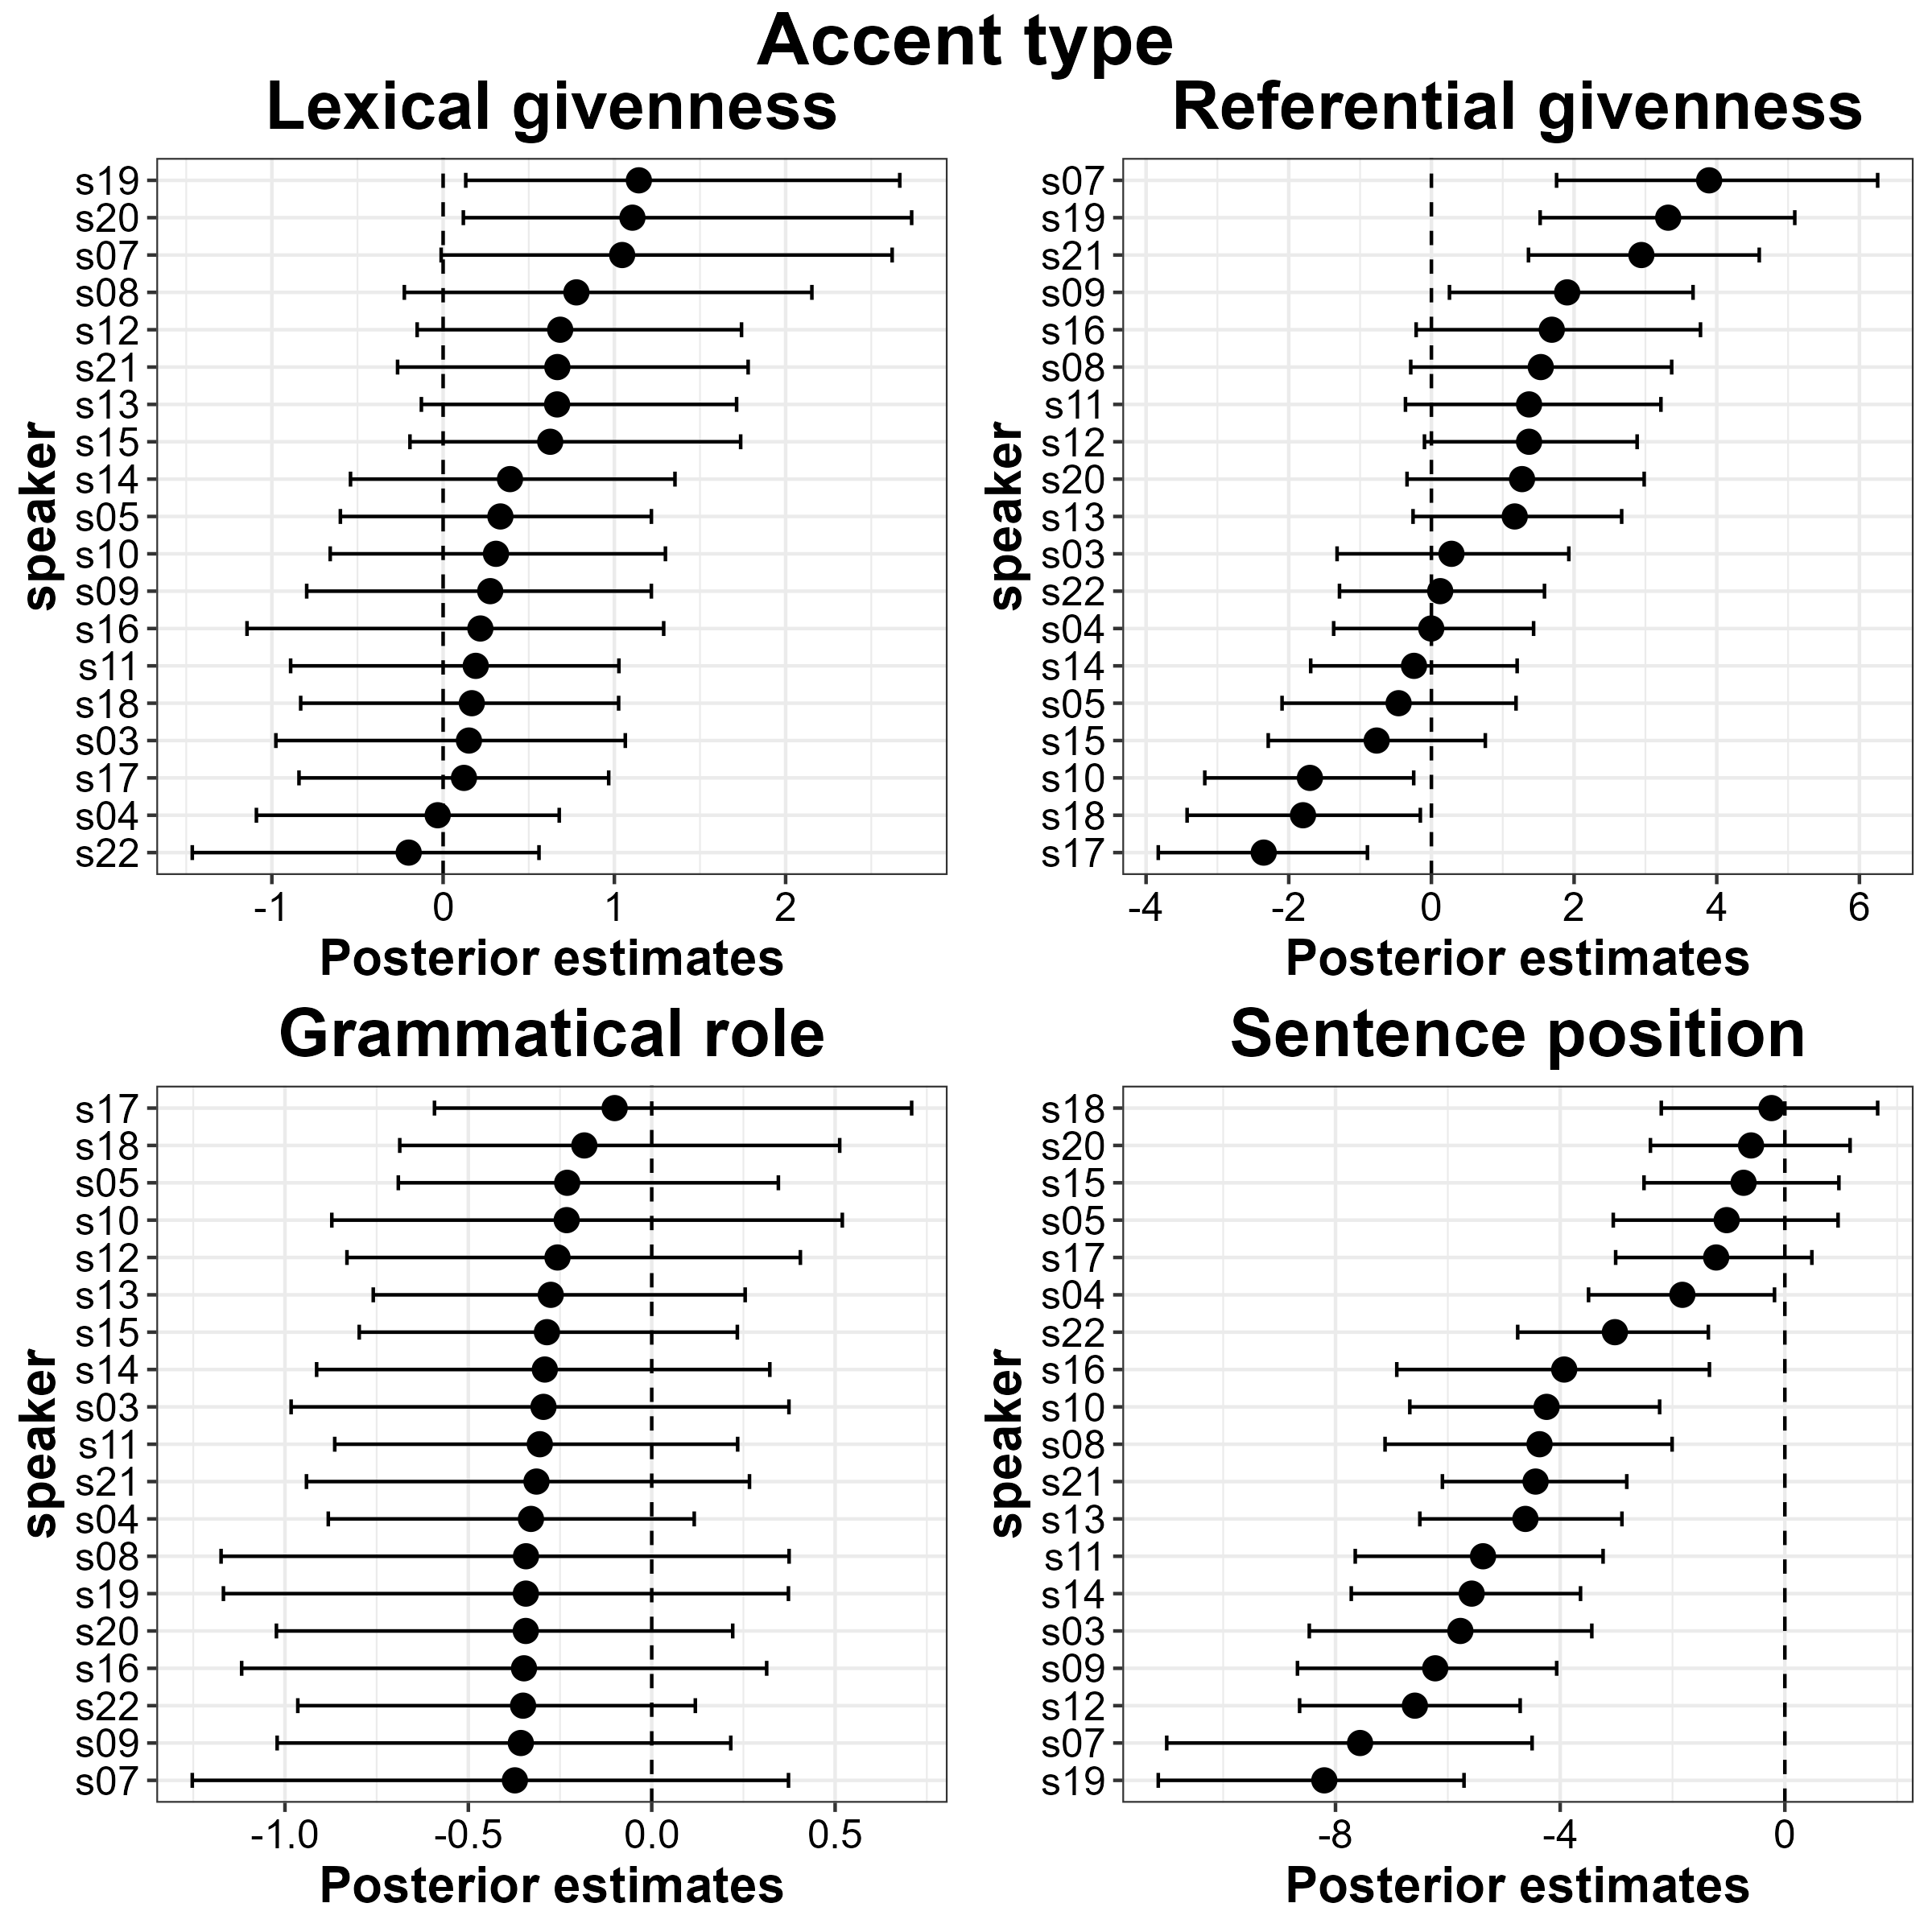
\includegraphics[scale = 0.5]{s2_accenttype_effects}
	\caption{Means and 90\% CrIs for the effects of lexical and referential givenness, grammatical role, and sentence position on accent type.}
	\label{fig:s2_accenttype_effects}
\end{figure}

To identify potential different strategies for the encoding of lexical and referential givenness, grammatical role, and sentence position via the continuous prosodic parameters, we run cluster analyses on the by-speaker random slopes extracted from the corresponding models (see Section \ref{sec:Production2 statistics} for details). For lexical givenness, the hierarchical cluster analysis suggests that a two cluster-solution is most appropriate for our data (silhouette width: 0.23). Cluster 1 contains twelve speakers and Cluster 2 contains seven speakers (see Figure \ref{fig:s2_clusters_lex}, left). Figure \ref{fig:s2_clusters_lex} (right) shows the average random slope values with 90\% CrIs for the effect of lexical givenness on the prosodic parameters per cluster. Here, a positive number indicates that l-new referents have a higher value than l-given referents in the parameter in question. The two clusters appear remarkably alike in their use of almost all parameters. The main difference between these two groups of speakers is the strength of encoding via syllable duration and periodic energy mass. Specifically, Cluster 2 marks a larger difference between l-new and l-given referents in terms of these two parameters. The same is true for F0 at CoM, word duration, and intensity, although the differences between the two clusters here are smaller. Overall, lexical givenness is thus very similarly encoded across speakers, which is supported by the low silhouette width value, indicating that there is only weak evidence for clustering potential in the data.

\begin{figure}
		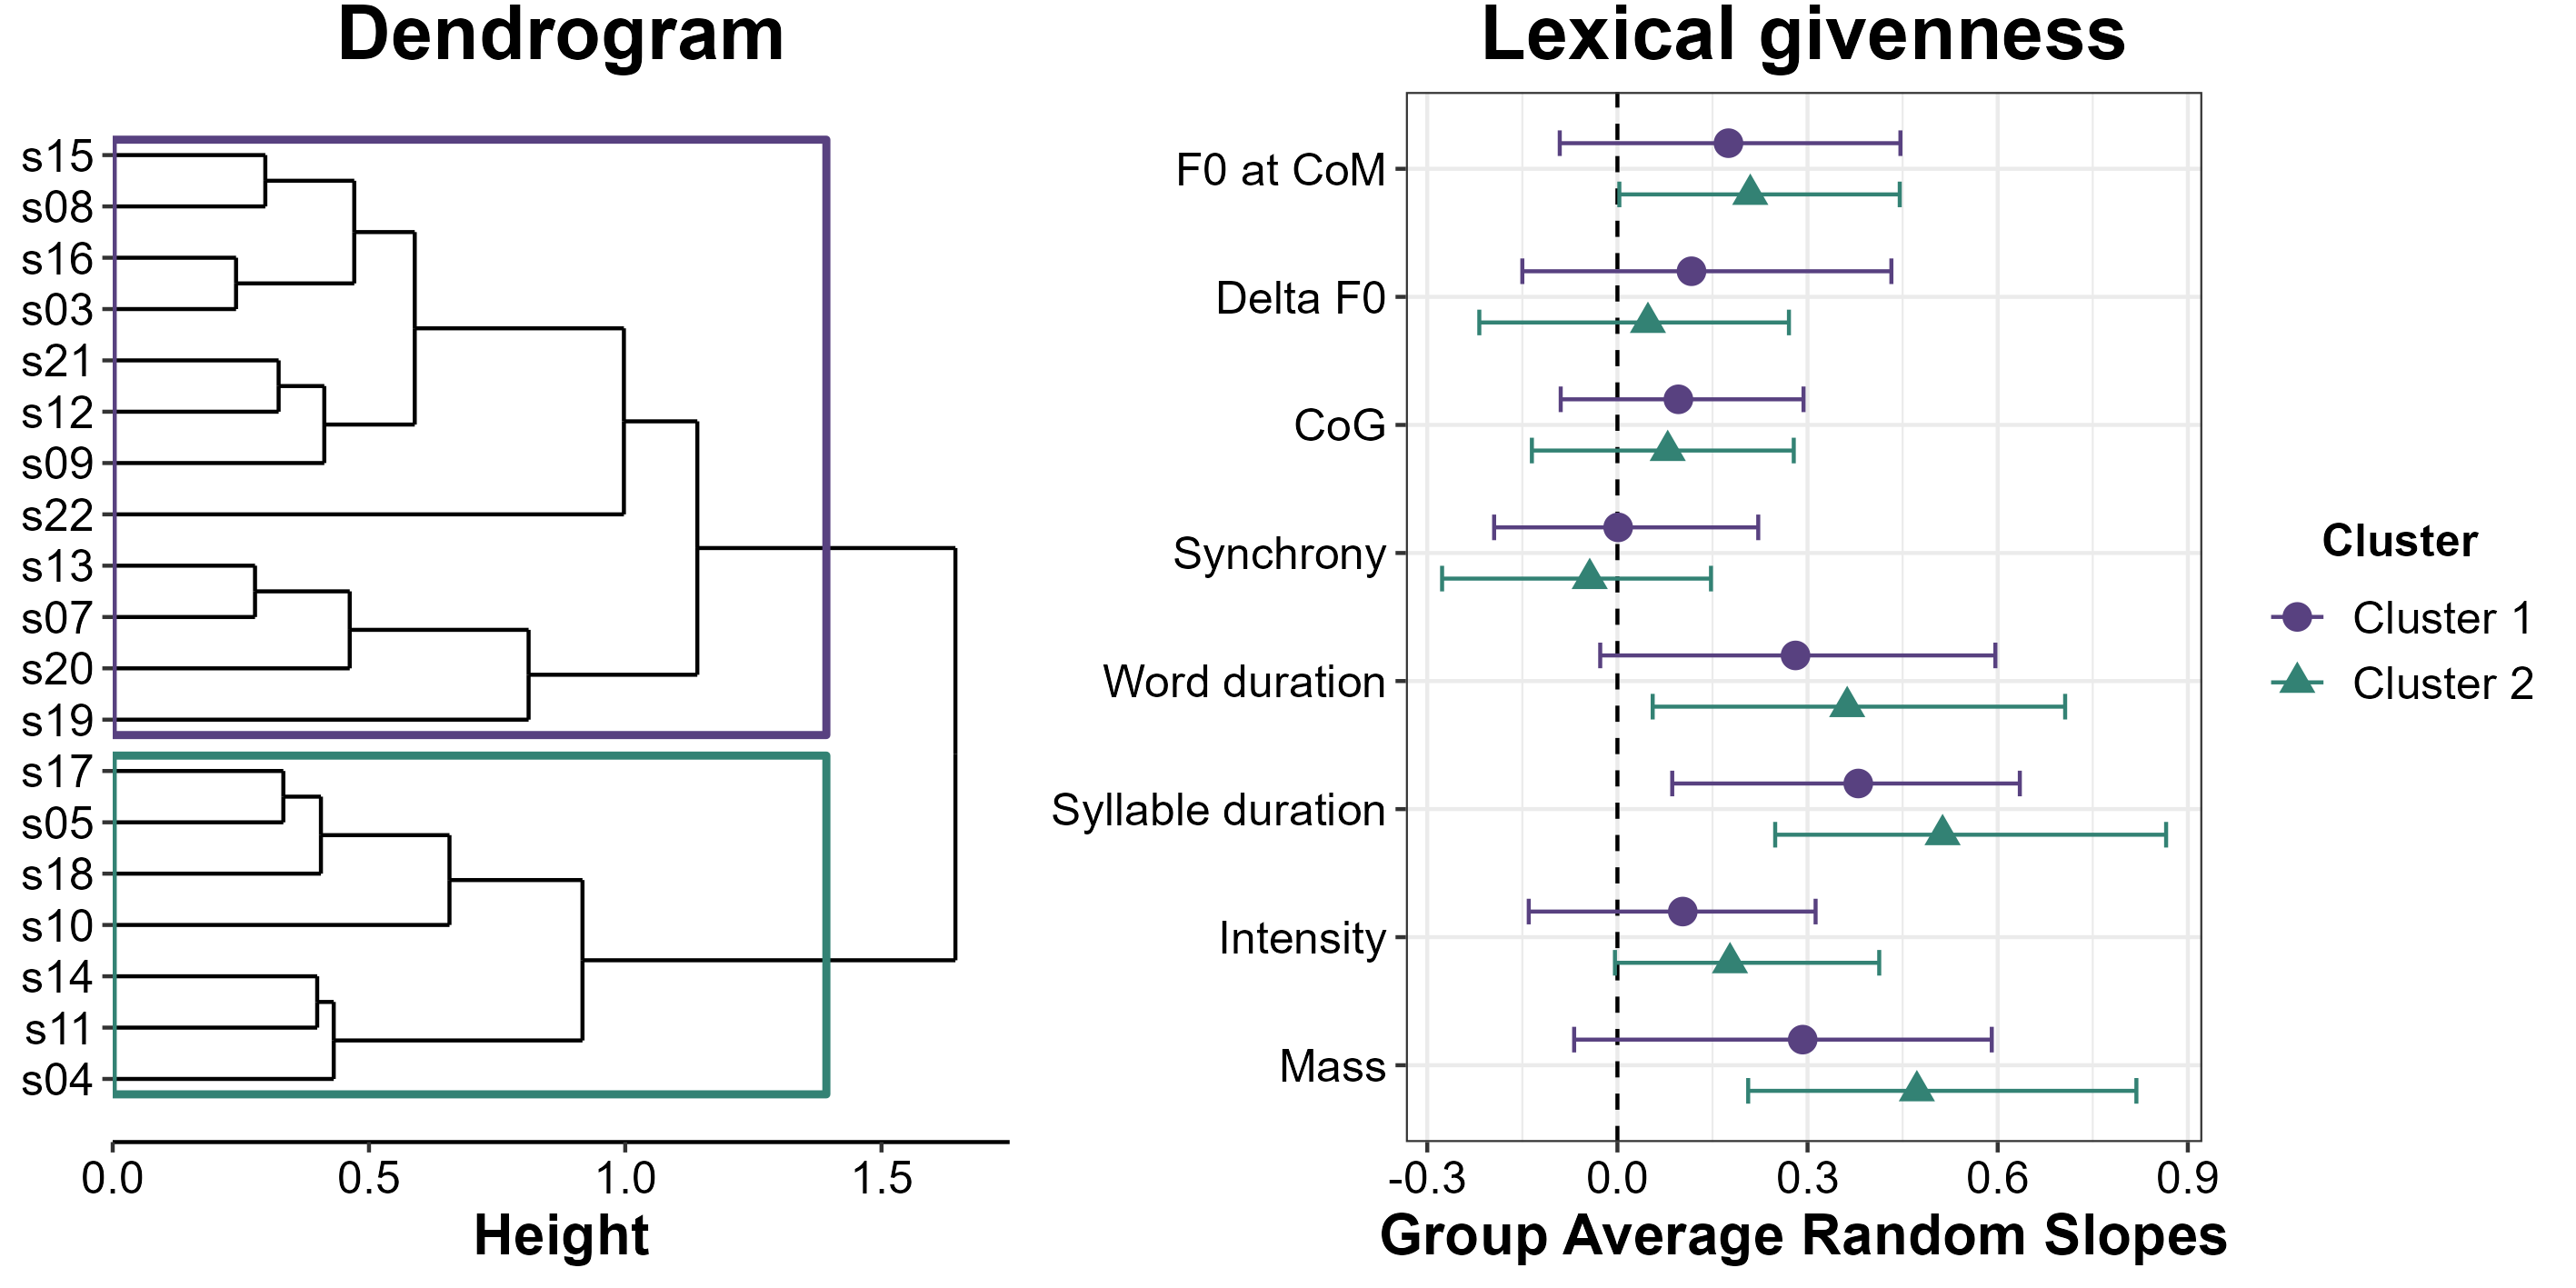
\includegraphics[scale = 0.5]{s2_clusters_lex}
	\caption{Results of cluster analysis for lexical givenness. Left: Dendrogram showing cluster affiliations of all speakers for lexical givenness. Right: Group averages and 90\% CrIs per cluster for each prosodic parameter.}
	\label{fig:s2_clusters_lex}
\end{figure}

Considering referential givenness, again two clusters of speakers emerge from the analysis (silhouette width: 0.34). Cluster 1 contains ten speakers while Cluster 2 contains nine speakers (see Figure \ref{fig:s2_clusters_ref}, left). Figure \ref{fig:s2_clusters_ref} (right) illustrates the characteristics of these two clusters. Here, the clusters converge on their use of word duration, syllable duration, intensity, and periodic energy mass. However, there appear to be differences in the modulation of F0 in r-new and r-given referents across the two clusters. In particular, Cluster 2 appears to produce r-new referents relatively consistently with higher F0 at the CoM and higher Delta F0 than r-given referents, whereas Cluster 1 does not make use of these two parameters in a reliable way. Meanwhile, Cluster 1 distinguishes more clearly between r-new and r-given referents in the F0 alignment, i.e., r-new referents are produced with lower CoG and lower synchrony values compared to r-given referents, while Cluster 2 only uses CoG in a similar way to a slightly lesser extent but not synchrony.

\begin{figure}
		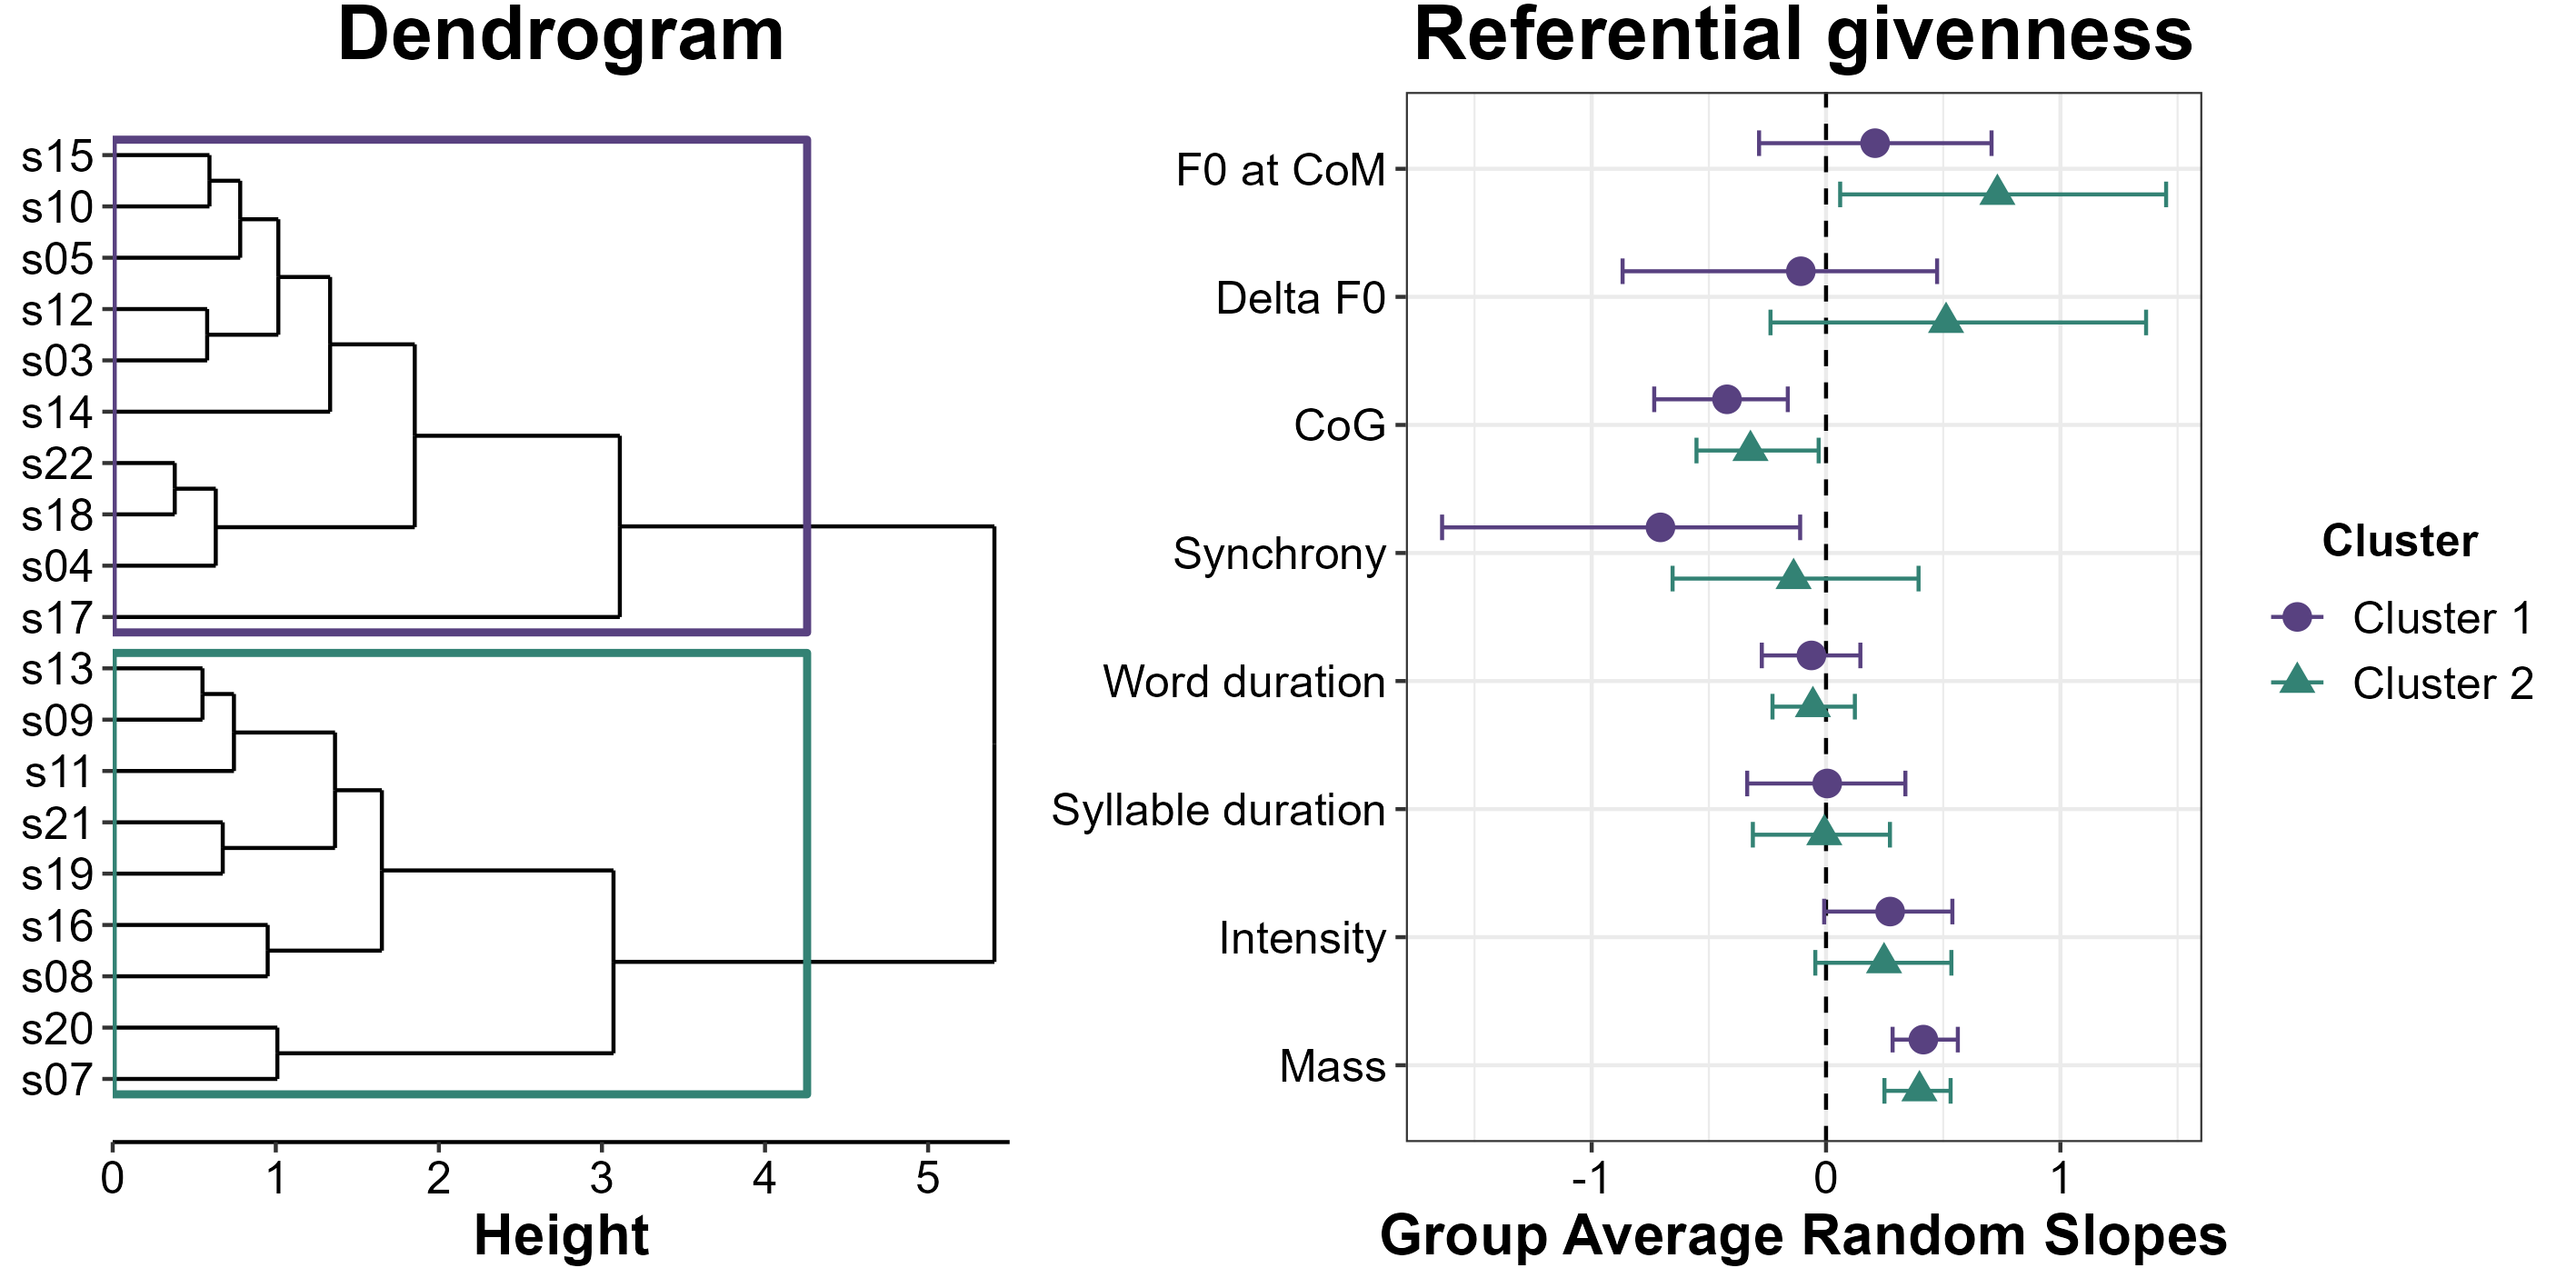
\includegraphics[scale = 0.5]{s2_clusters_ref}
	\caption{Results of cluster analysis for referential givenness. Left: Dendrogram showing cluster affiliations of all speakers for referential givenness. Right: Group averages and 90\% CrIs per cluster for each prosodic parameter.}
	\label{fig:s2_clusters_ref}
\end{figure}

Turning next to the encoding of grammatical role, the cluster analysis indicates that a split into three groups is most appropriate for our data (silhouette width: 0.37). Cluster 1 contains seven speakers, Cluster 2 four speakers, and Cluster 3 eight speakers (see Figure \ref{fig:s2_clusters_gramm}, left). Looking at the characteristics of these three clusters in Figure \ref{fig:s2_clusters_gramm} (right), clusters again behave very similarly in their use of most parameters, e.g., F0 at CoM, Delta F0, and periodic energy mass. The most obvious difference across clusters is in regards to CoG. While Cluster 3 barely modifies CoG between objects and subjects, Cluster 1 clearly produces an earlier CoG in objects, with Cluster 2 falling in between these two behaviors. 

\begin{figure}[t]
		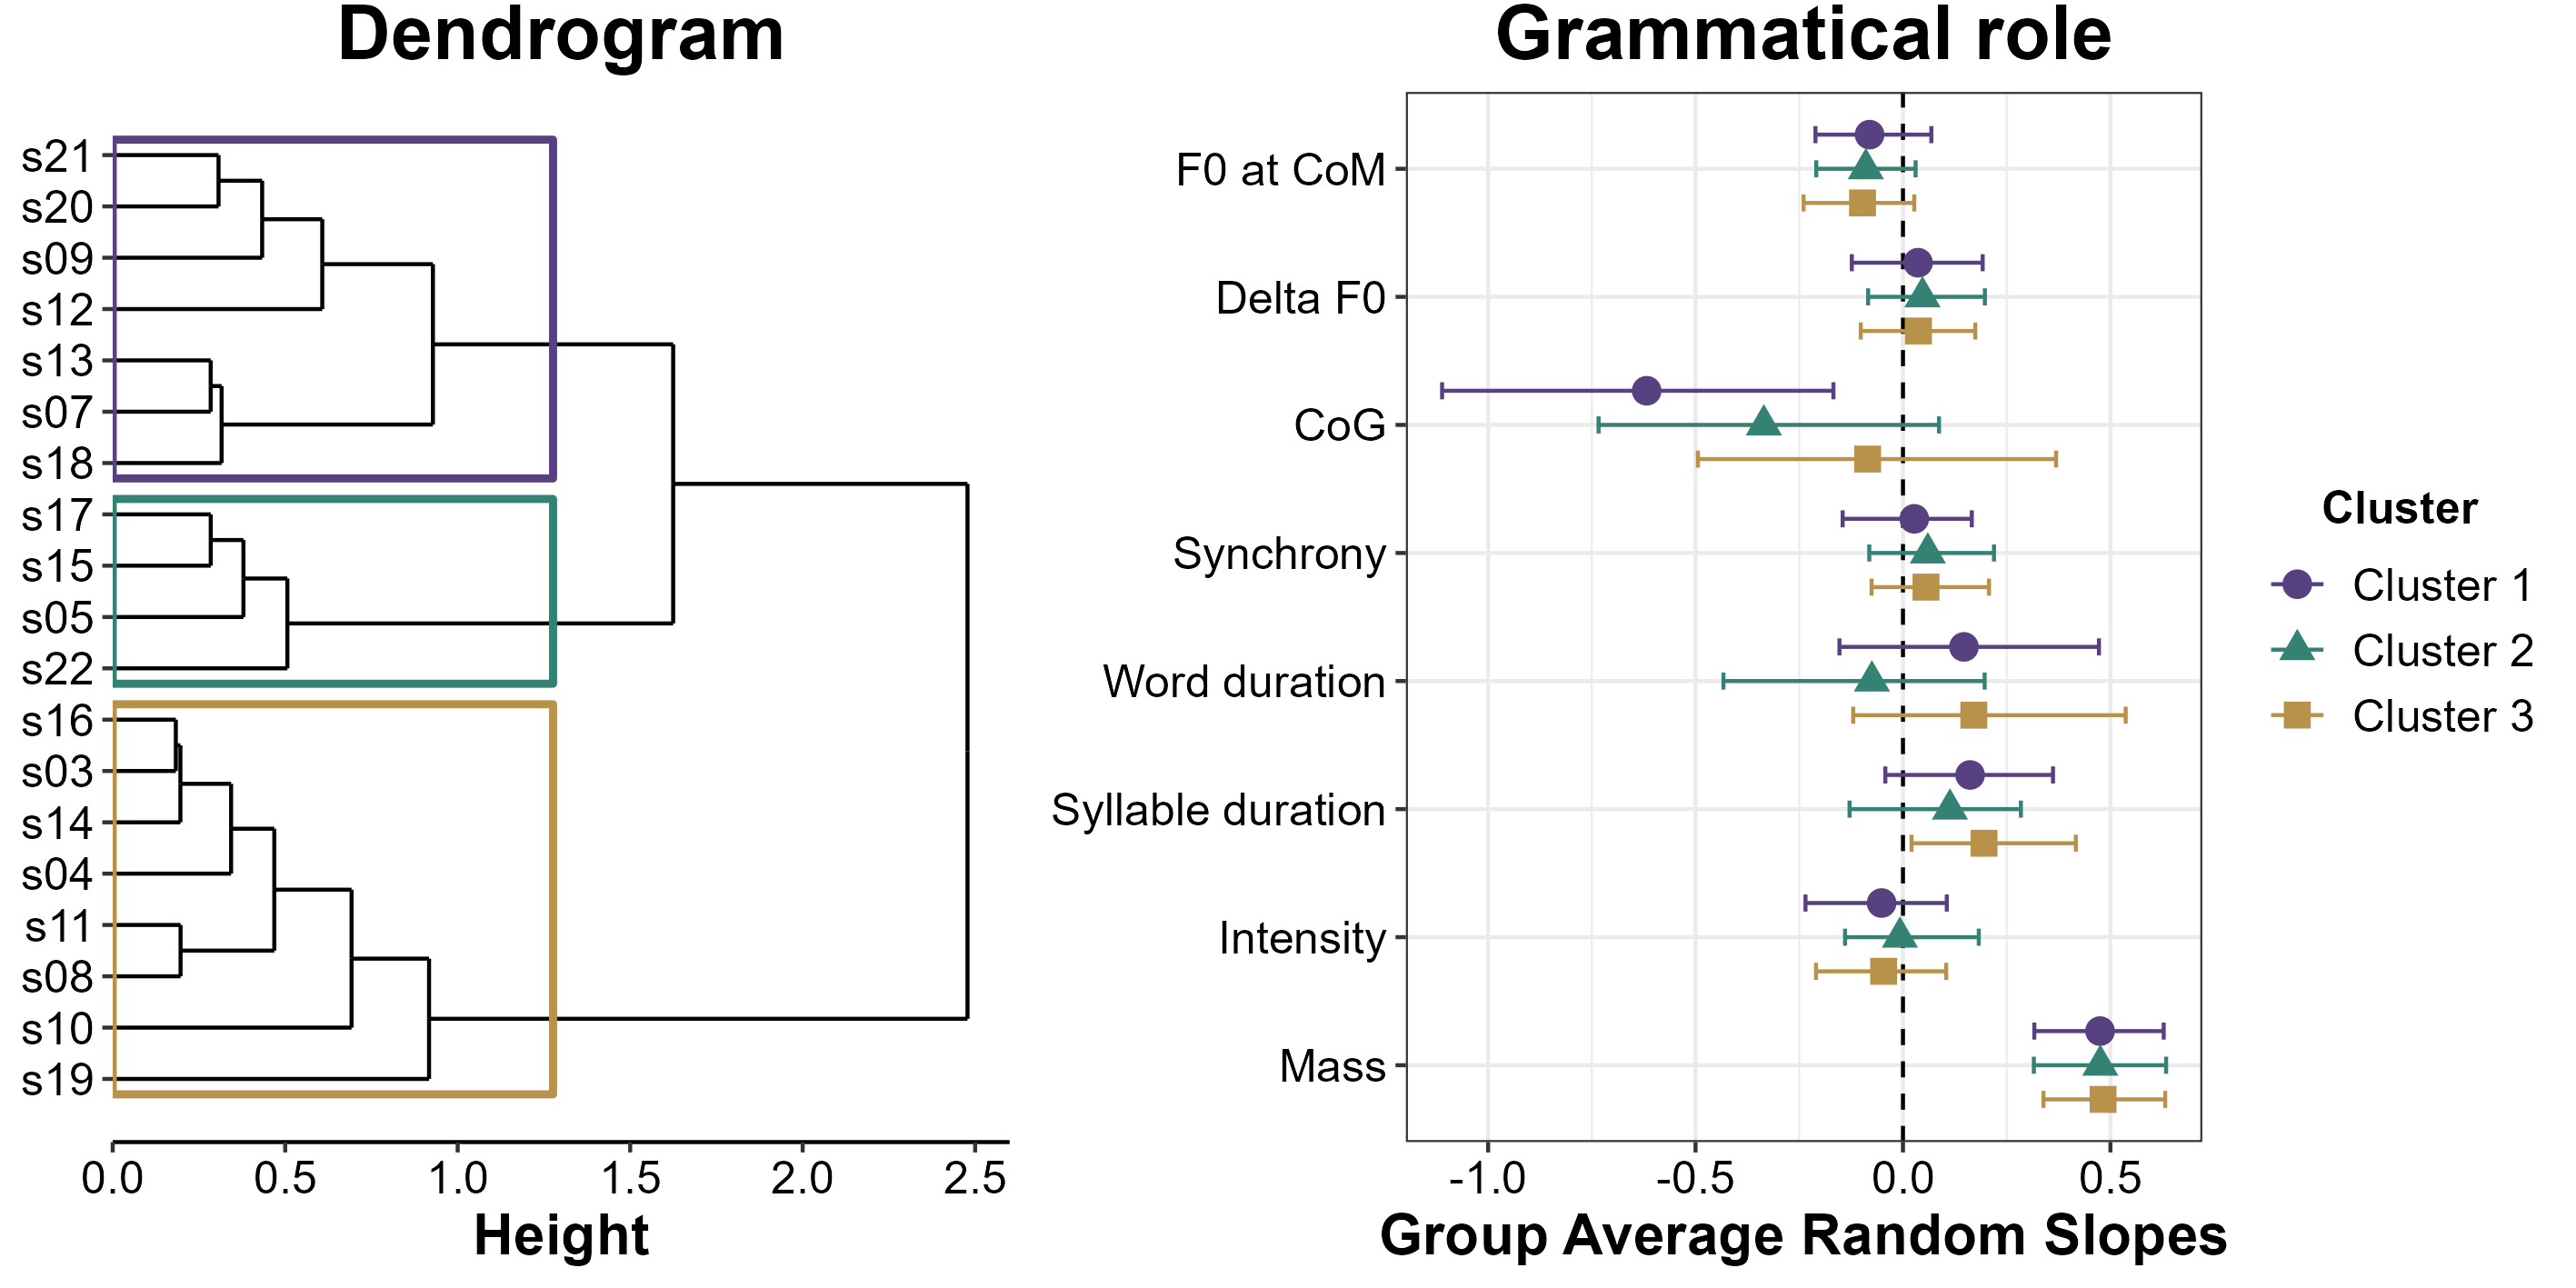
\includegraphics[scale = 0.5]{s2_clusters_gramm}
	\caption{Results of cluster analysis for grammatical role. Left: Dendrogram showing cluster affiliations of all speakers for grammatical role. Right: Group averages and 90\% CrIs per cluster for each prosodic parameter.}
	\label{fig:s2_clusters_gramm}
\end{figure}

Sentence position appears to give rise to the most variability across speakers, with the cluster analysis suggesting a partitioning into five clusters as optimal (silhouette width: 0.31). Accordingly, the individual clusters are smaller, with Cluster 1 containing four speakers, Cluster 2 five speakers, Cluster 3 six speakers, Cluster 4 three speakers, and Cluster 5 only one speaker (see Figure \ref{fig:s2_clusters_pos}, left). Judging from the CrIs' distance to the vertical zero line, it is evident that all clusters reliably differentiate between initial and medial target words in terms of synchrony, word duration, syllable duration, intensity, and periodic energy mass, albeit to differing extents (see Figure \ref{fig:s2_clusters_pos}, right). Nevertheless, there is some variability with regard to F0 at CoM, Delta F0, and CoG. Of these three, Cluster 1 appears to only use CoG, Cluster 2 and 3 use F0 at CoM and Delta F0, and Cluster 4 and 5 use all three to encode sentence position prosodically. There are also more gradient differences across these clusters, with Cluster 2 producing generally larger differences between initial and medial words than Cluster 3, and Cluster 5 (i.e., speaker s09) producing larger differences than Cluster 4.

\begin{figure}
		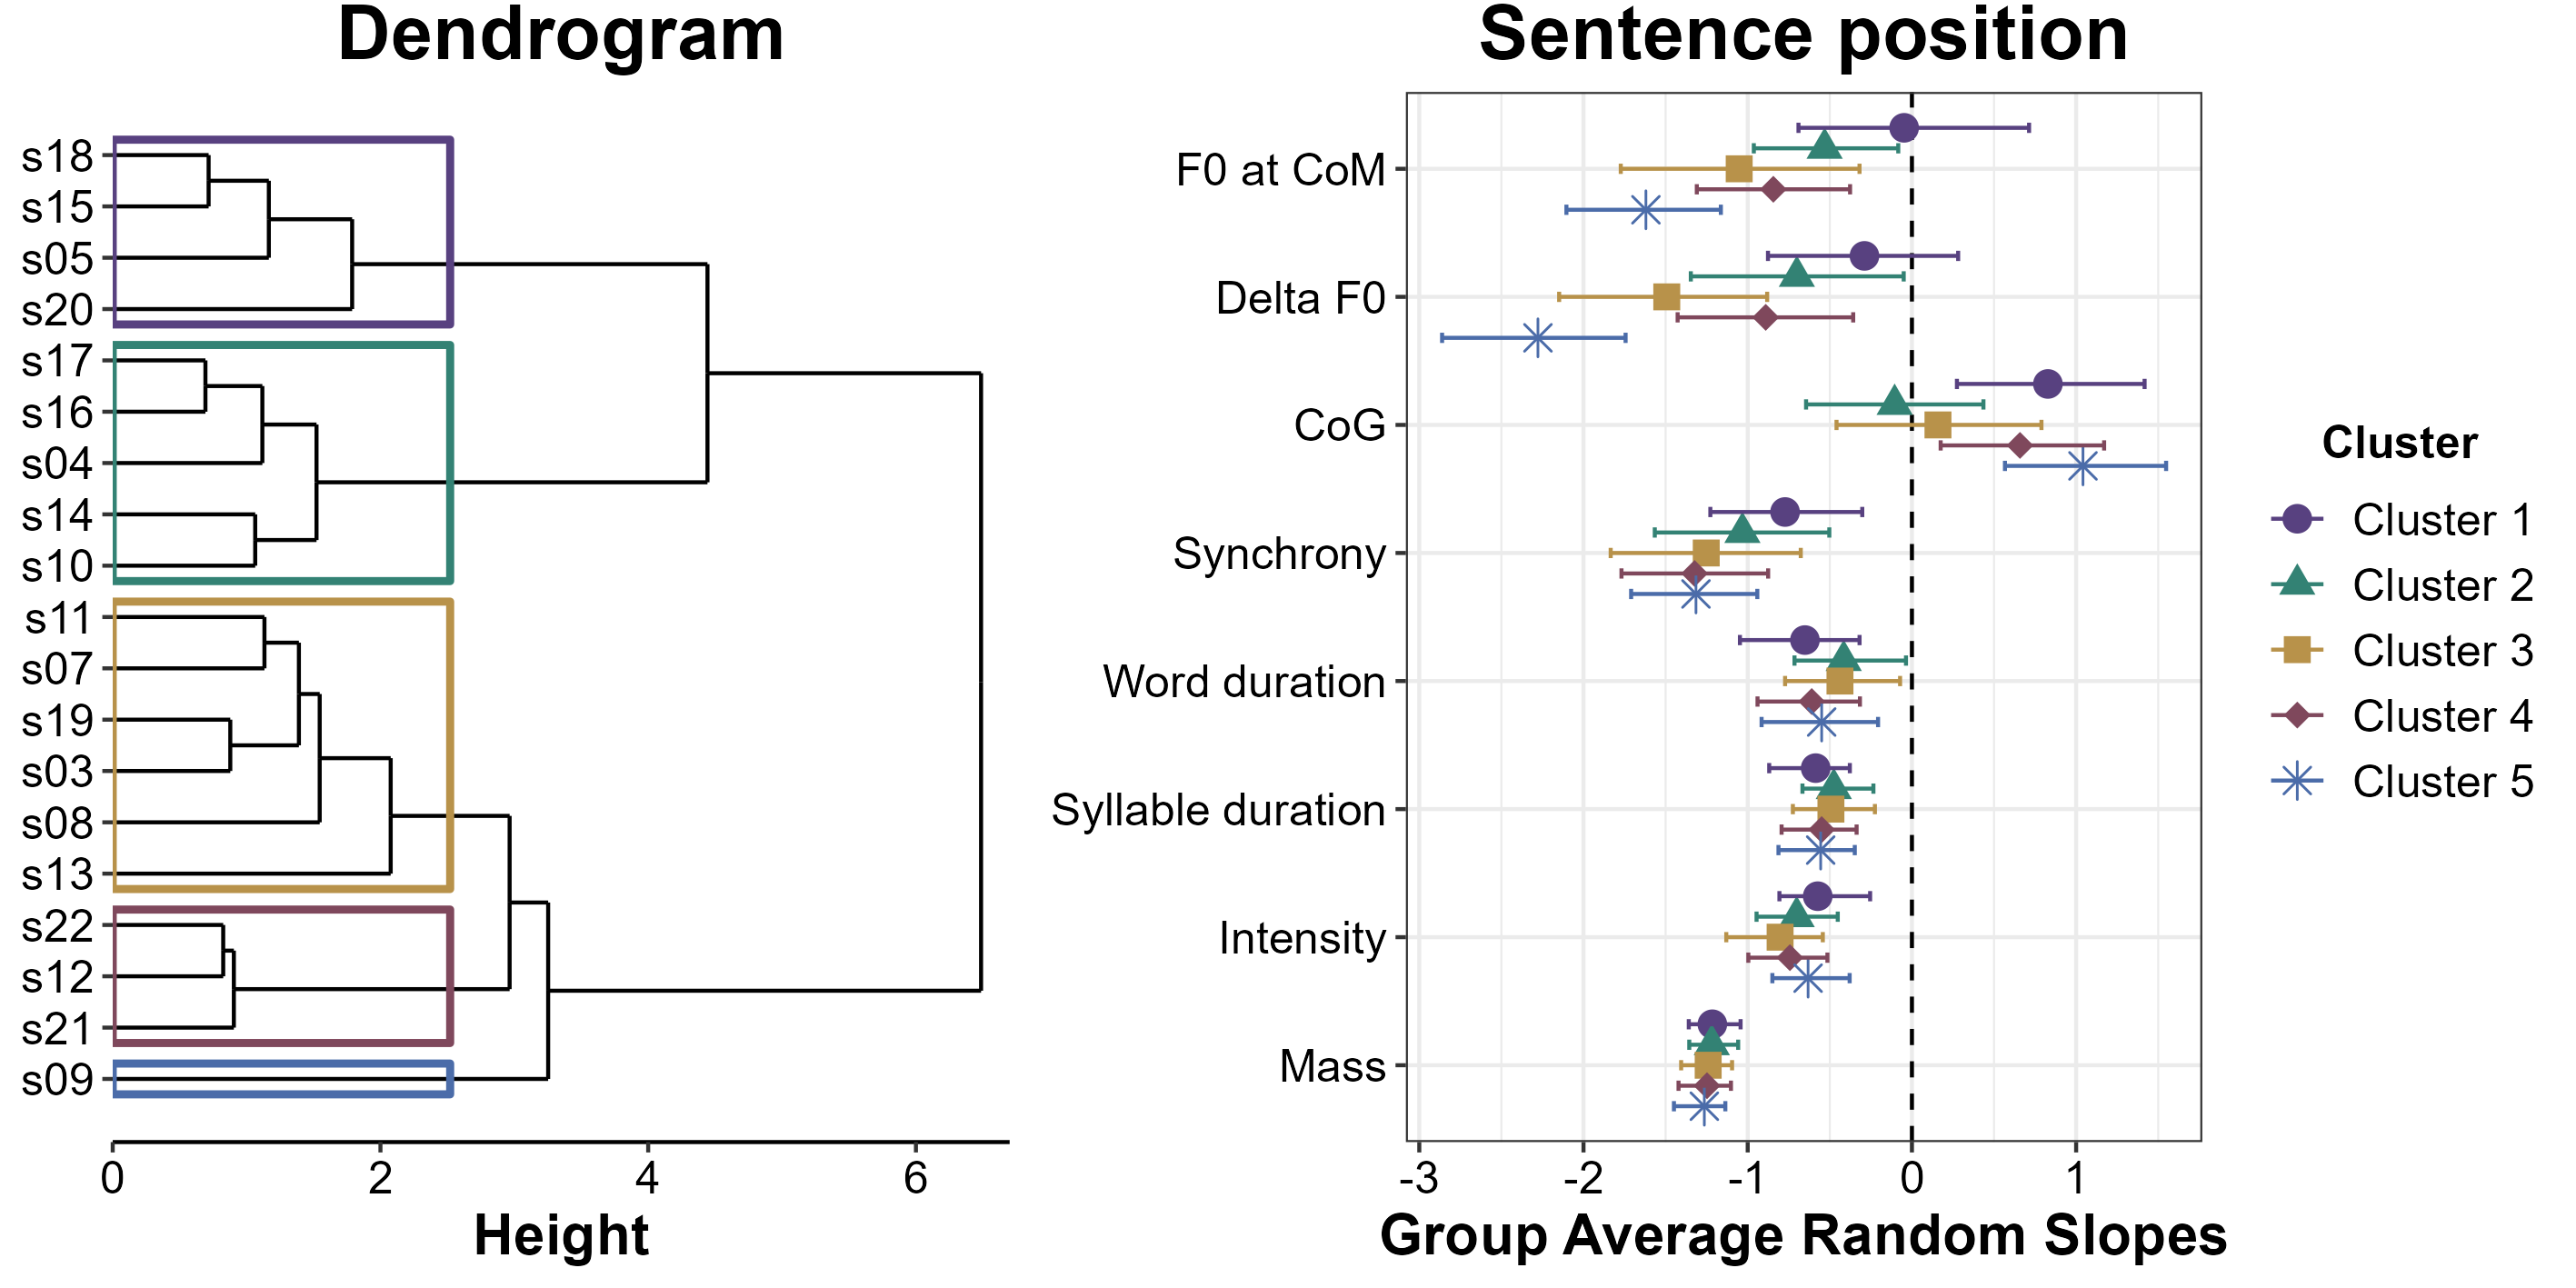
\includegraphics[scale = 0.5]{s2_clusters_pos}
	\caption{Results of cluster analysis for sentence position. Left: Dendrogram showing cluster affiliations of all speakers for sentence position. Right: Group averages and 90\% CrIs per cluster for each prosodic parameter.}
	\label{fig:s2_clusters_pos}
\end{figure}

To integrate the findings of the categorical and continuous parameters, we plot the number of speakers using or not using accent status and accent type as cues to each of the semantic-pragmatic and syntactic factors under investigation by their cluster affiliations. We classify a speaker as a user of accent status or type when the 90\% CrI of their corresponding random slope does not include zero (see Figures \ref{fig:s2_accentstatus_effects} and \ref{fig:s2_accenttype_effects}). First, lexical givenness is reliably encoded by accent status and accent type only by a few speakers, so that it is difficult to identify systematic behavior by any of the two clusters (see Figure \ref{fig:s2_accent_statustype_bycluster_lex}). In Cluster 1, there are two speakers using accent status and two other speakers using accent type to cue lexical givenness. Similarly, in Cluster 2, two speakers use accent status, however, none are users of accent type. Proportionally, with Cluster 2 containing fewer speakers overall, speakers affiliated with Cluster 2 are more likely to use accent status than speakers in Cluster 1. This finding corresponds to the observation that Cluster 2 also makes stronger use of the continuous parameters than Cluster 1, especially those related to duration and intensity. For accent type, the relation is reversed, with more speakers in Cluster 1 making use of different accent types to mark lexical givenness. Overall, the two clusters are very similar in their encoding of lexical givenness in both their modulation of categorical and continuous prosodic parameters. 

\begin{figure}
		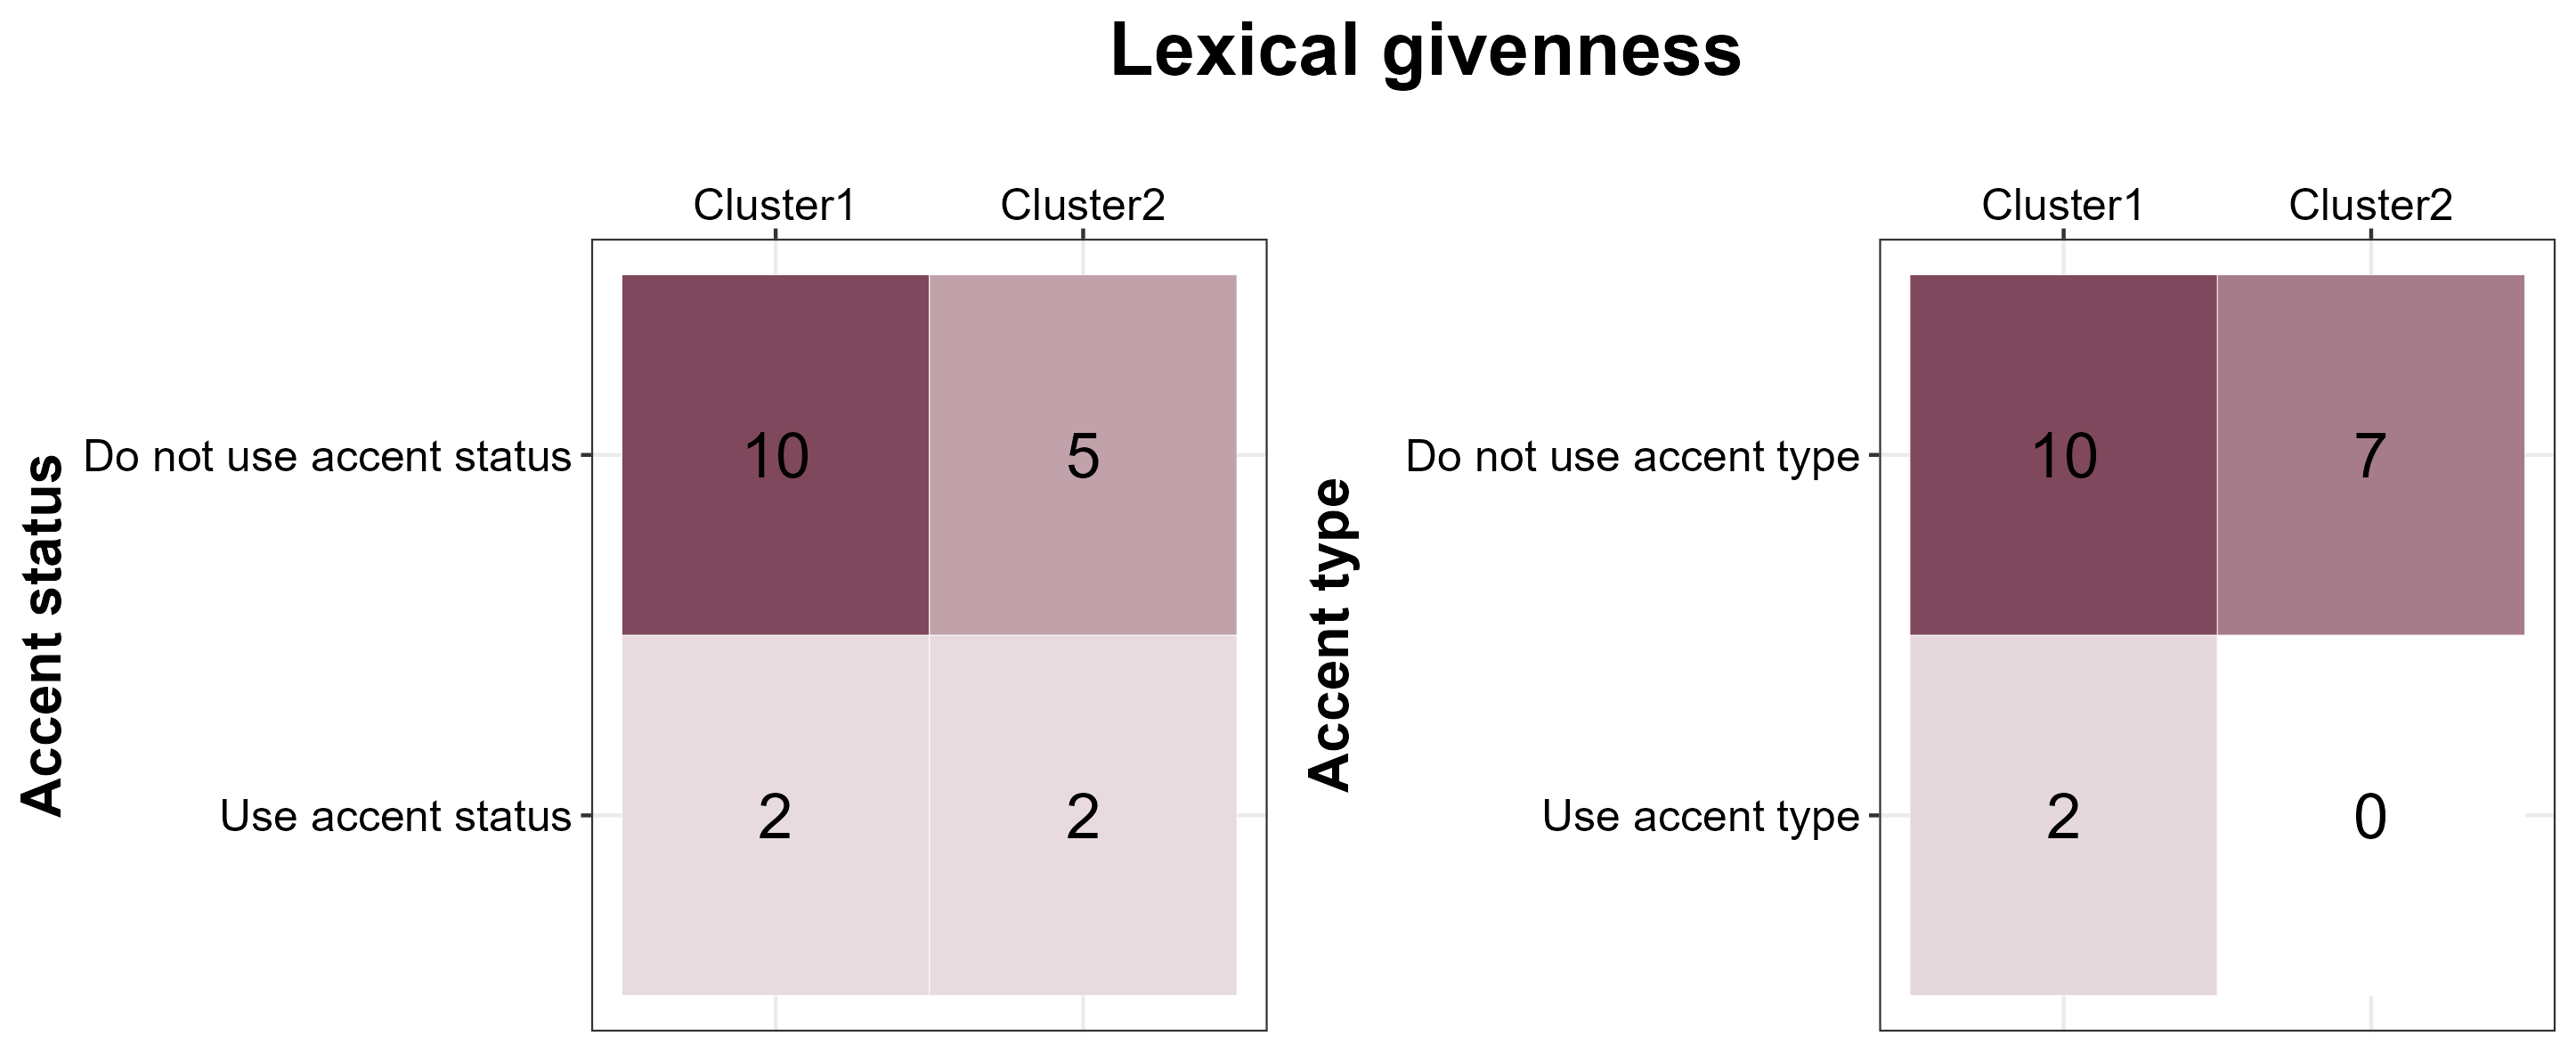
\includegraphics[scale = 0.5]{s2_accent_statustype_bycluster_lex}
	\caption{Plot showing the number of speakers using accent status (left) and accent type (right) to encode lexical givenness as a function of their cluster.}
	\label{fig:s2_accent_statustype_bycluster_lex}
\end{figure}

For referential givenness, a more interesting picture emerges. As evident from Figure \ref{fig:s2_accent_statustype_bycluster_ref}, most speakers reliably use accent status as a cue to referential givenness, regardless of their cluster affiliation. In contrast, none of the speakers in Cluster 1 uses more prominent accent types to mark r-new words. However, three speakers from this cluster produce the opposite pattern, with more prominent accent types on r-given words. This pattern is unattested in Cluster 2. Instead, about half of the speakers in Cluster 2 do not use accent type to mark referential givenness, but the other half makes use of accent type in the expected direction. This latter observation is also reflected in some of the continuous F0 measures, most notably F0 at CoM and Delta F0, which are used to a larger extent by Cluster 2 than by Cluster 1.

\begin{figure}
		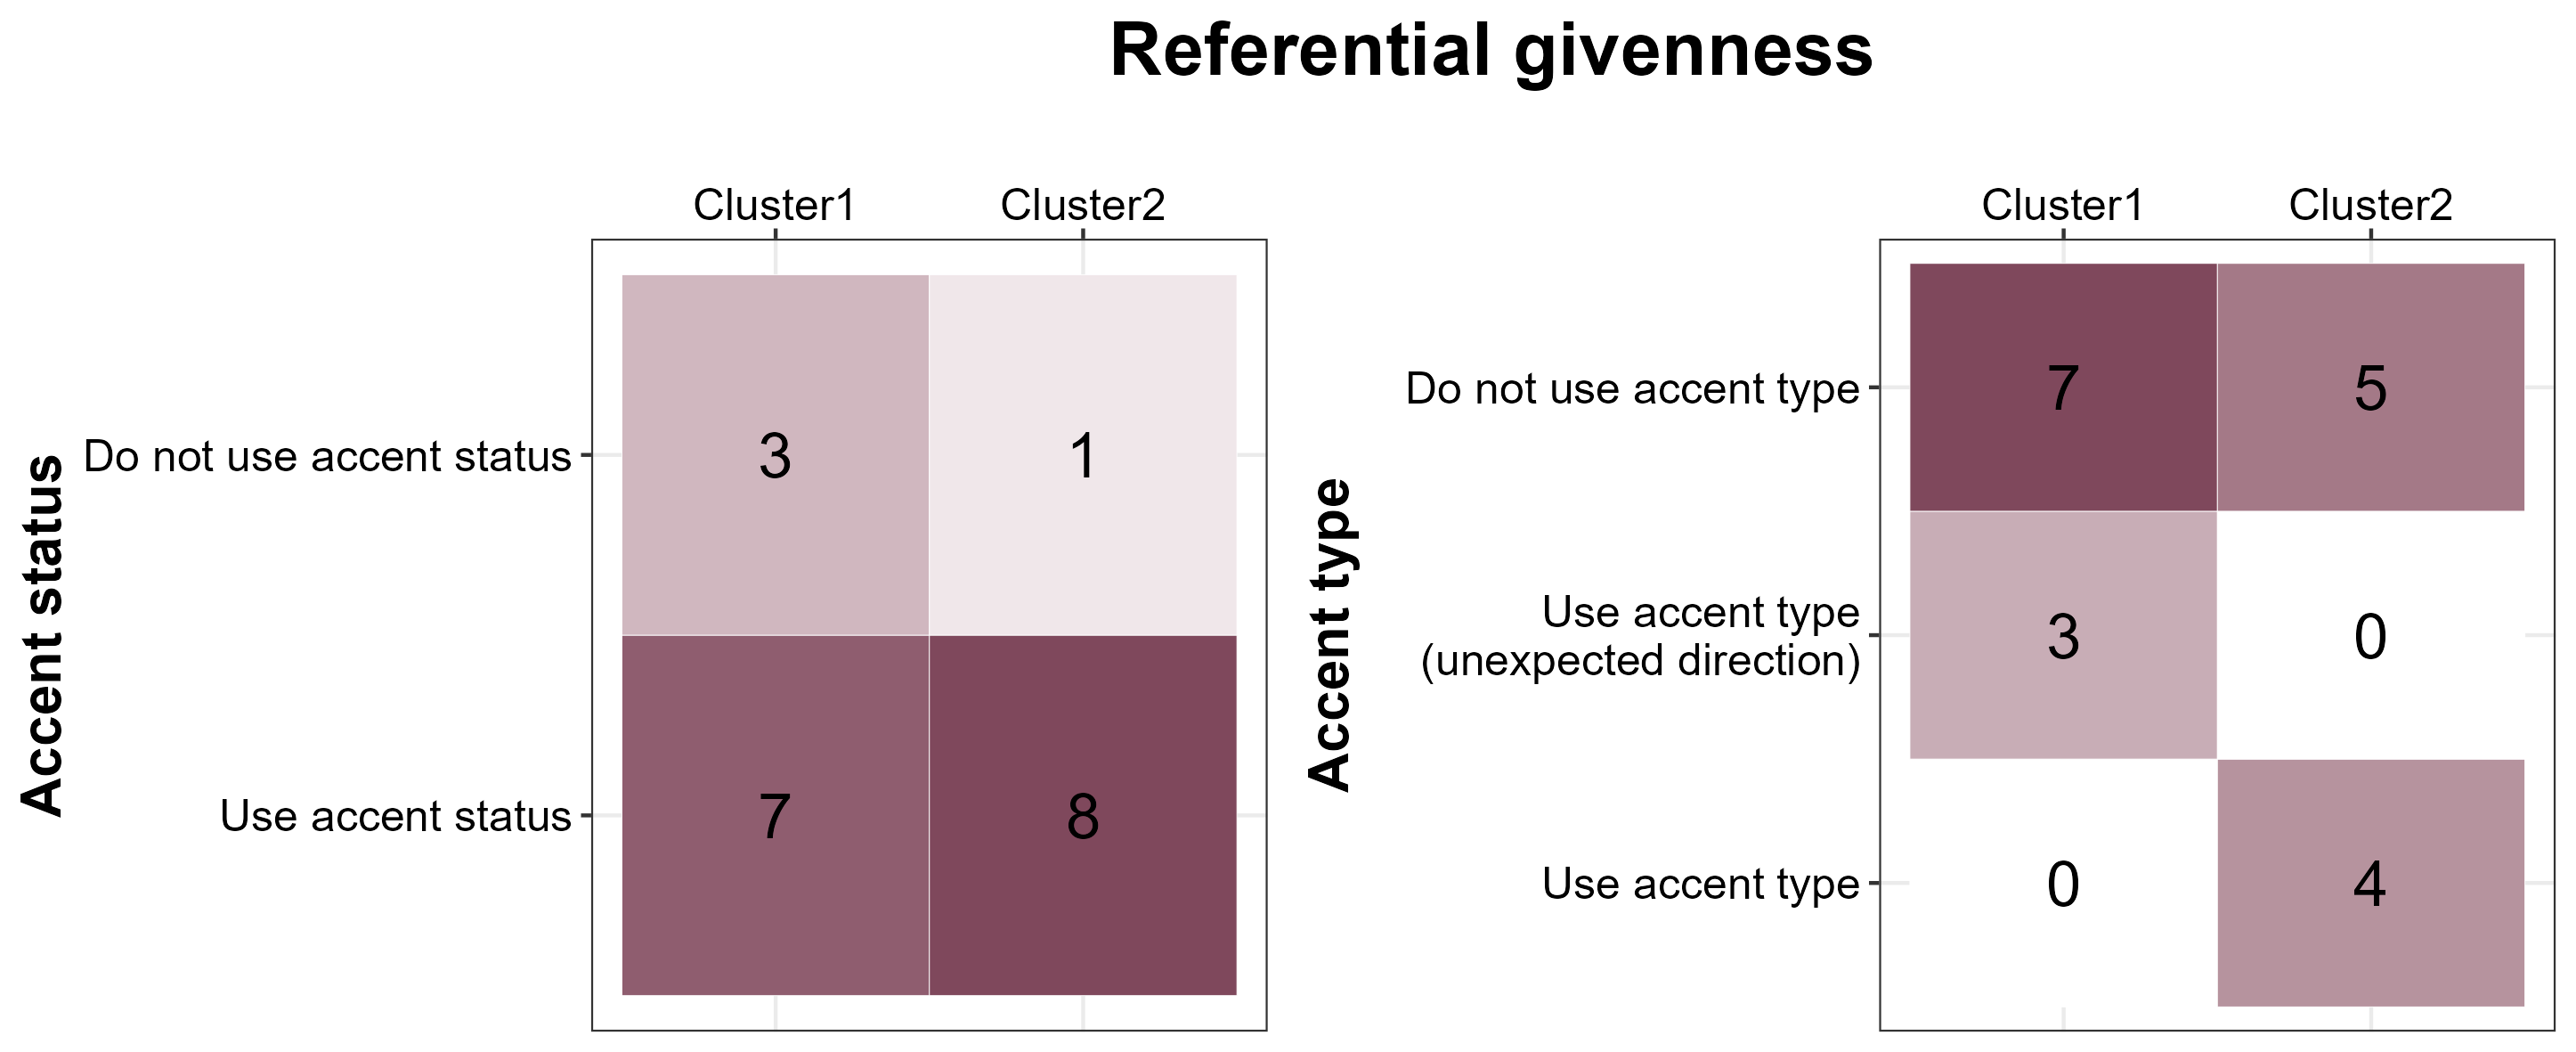
\includegraphics[scale = 0.5]{s2_accent_statustype_bycluster_ref}
	\caption{Plot showing the number of speakers using accent status (left) and accent type (right) to encode referential givenness as a function of their cluster.}
	\label{fig:s2_accent_statustype_bycluster_ref}
\end{figure}

The three clusters that emerged from the analysis of the encoding of grammatical role pattern very clearly with regard to their use of accent status and accent type (see Figure \ref{fig:s2_accent_statustype_bycluster_gramm}). While Cluster 1 and Cluster 2 rely on accent status but not accent type to mark objects as more prominent than subjects, the majority of speakers in Cluster 3 uses neither of the categorical parameters to this end. In contrast to the findings on lexical and referential givenness, these observations do not directly relate to the findings with regard to the continuous parameters, suggesting that categorical and continuous parameters may also act independently to some degree. 

\begin{figure}[t]
		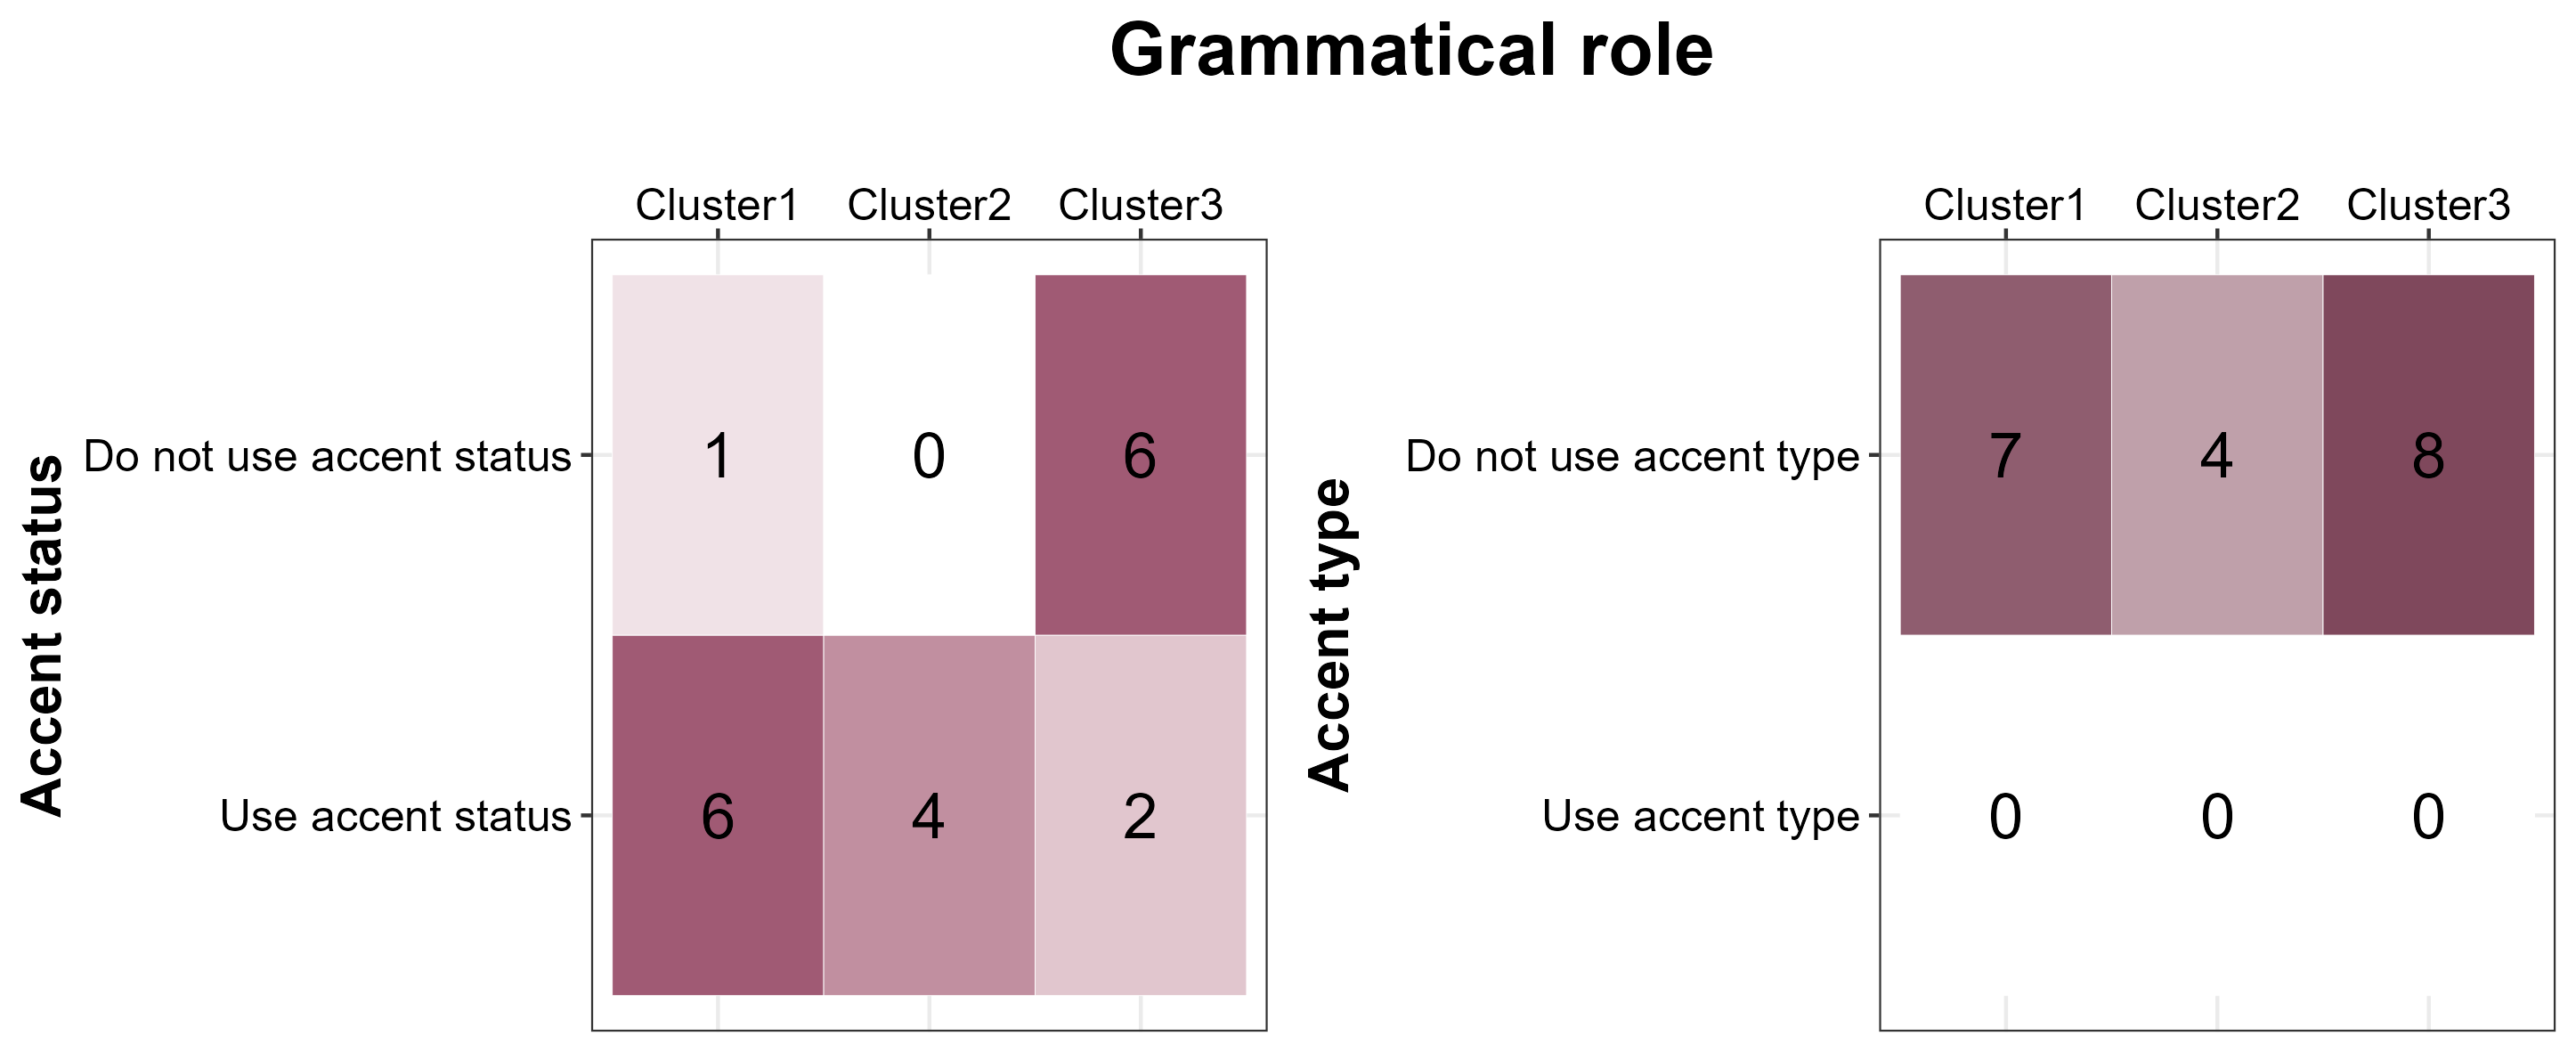
\includegraphics[scale = 0.5]{s2_accent_statustype_bycluster_gramm}
	\caption{Plot showing the number of speakers using accent status (left) and accent type (right) to encode grammatical role as a function of their cluster.}
	\label{fig:s2_accent_statustype_bycluster_gramm}
\end{figure}

Finally, for sentence position, a mostly complementary pattern emerges across clusters (see Figure \ref{fig:s2_accent_statustype_bycluster_pos}). While Cluster 1 uses accent status but not accent type to mark initial target words as more prominent than medial words, the reverse is true for Cluster 2, Cluster 3, and Cluster 4, where the majority of speakers use accent type but not accent status. The single speaker in Cluster 5 provides an exception to the complementary pattern, making use of both accent status and accent type. In line with this observation, the speaker in Cluster 5 also distinguishes most clearly between the initial and medial positions in terms of continuous parameters. The use of accent type correlates nicely with higher mean F0 at CoM and Delta F0 for initial words produced by speakers in Cluster 2, Cluster 3, Cluster 4, and Cluster 5 compared to Cluster 1.

\begin{figure}[t]
		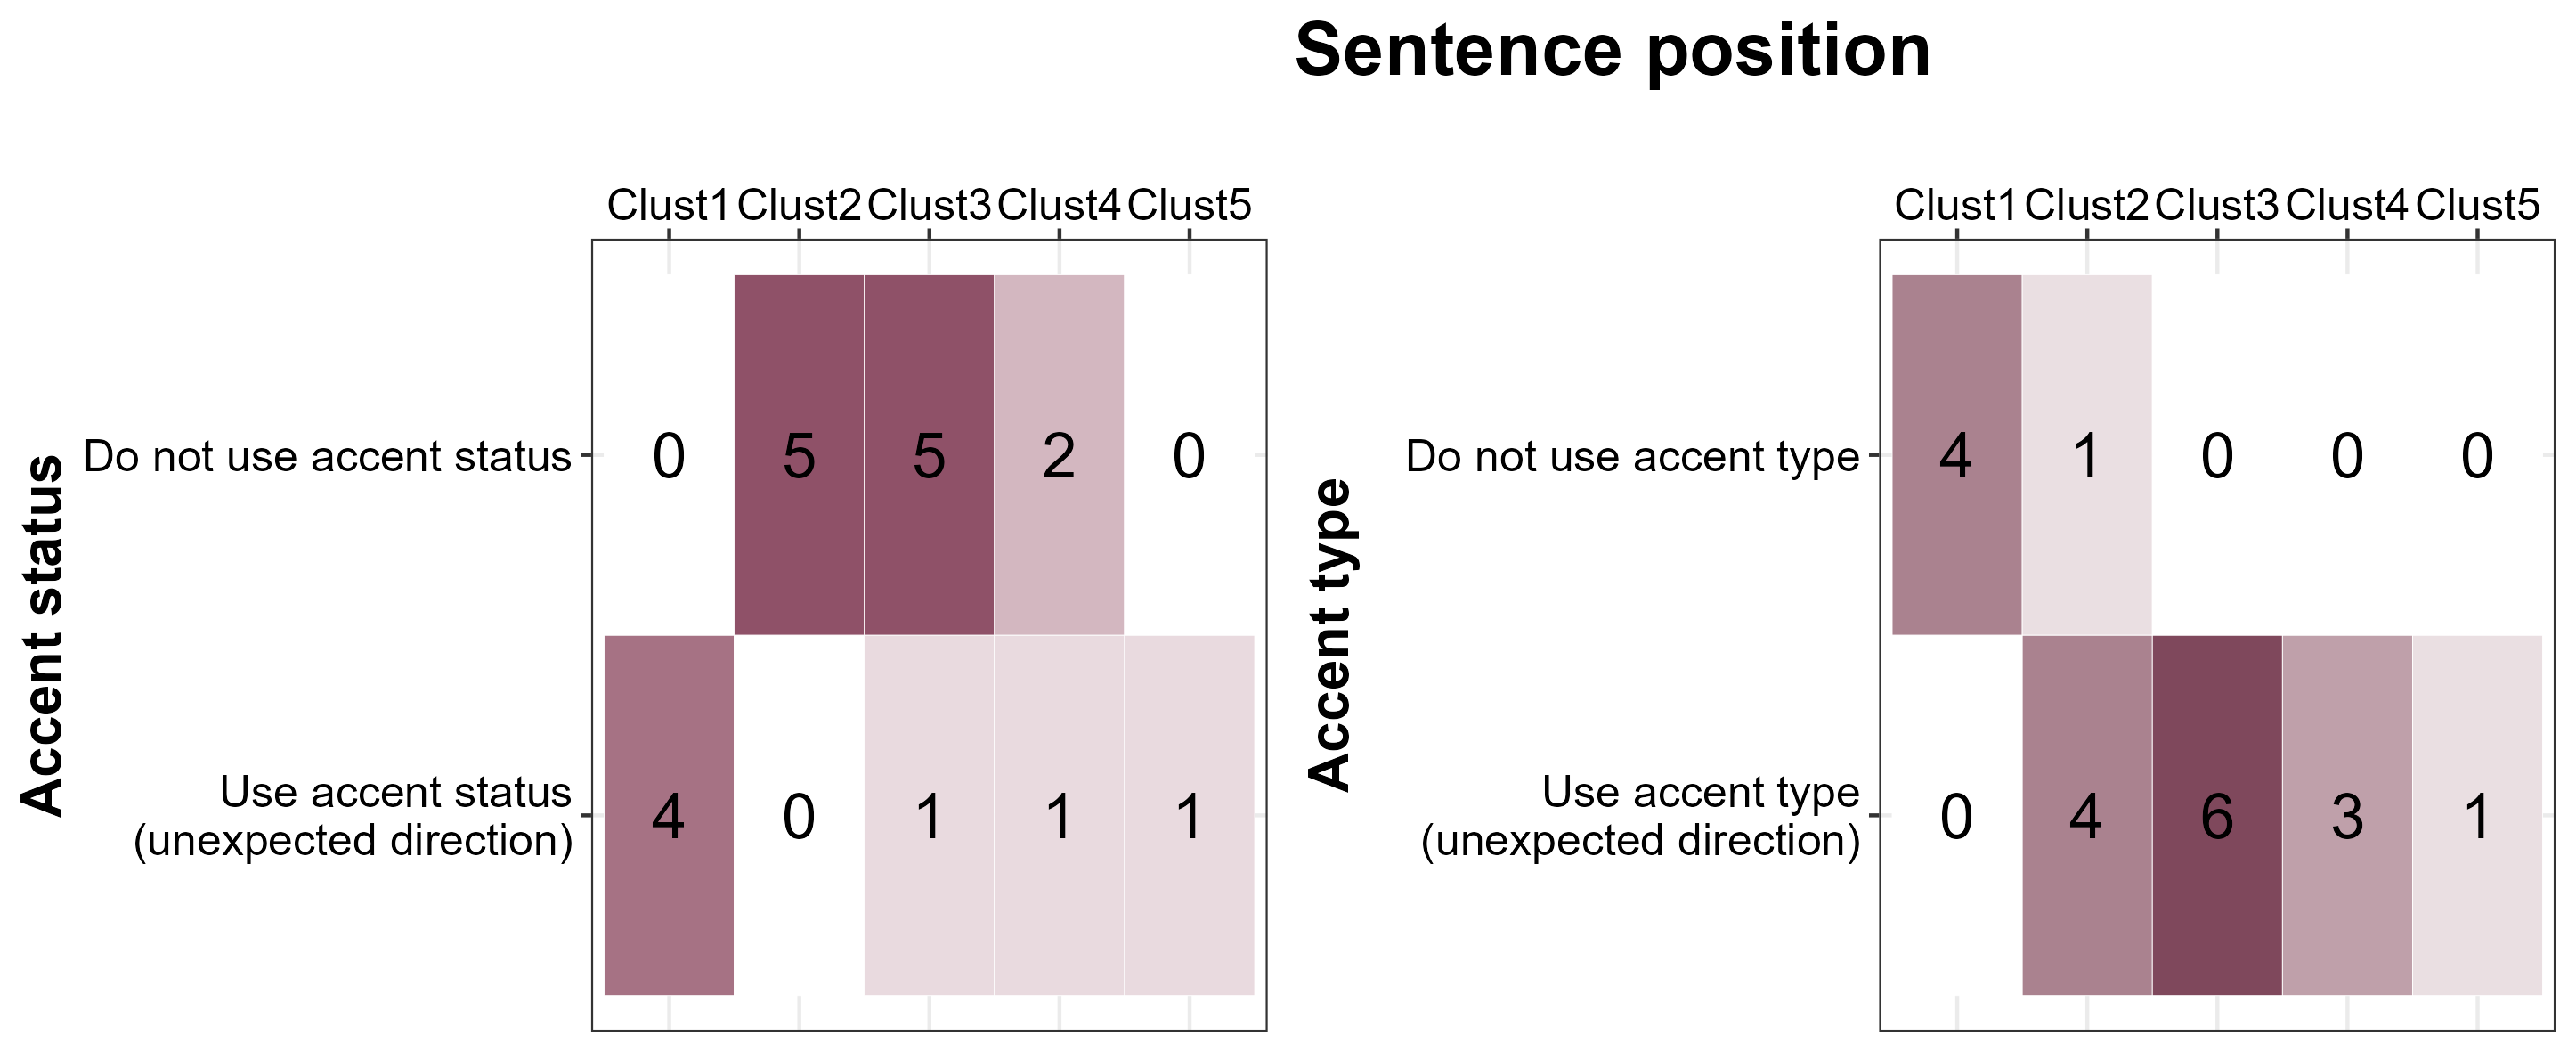
\includegraphics[scale = 0.5]{s2_accent_statustype_bycluster_pos}
	\caption{Plot showing the number of speakers using accent status (left) and accent type (right) to encode sentence position as a function of their cluster.}
	\label{fig:s2_accent_statustype_bycluster_pos}
\end{figure}

Generally, continuous parameters reflect categorical ones relatively well, so that clustering performed on the continuous parameters corresponds to patterns in terms of categorical parameters across speakers.

Before turning to potential effects of communicative skill, we briefly note on the sociodemographic characteristics of the speakers in the reported clusters. For lexical givenness, we identified two clusters, the weaker encoders (Cluster 1) and the stronger encoders (Cluster 2). Speakers in Cluster 1 are on average slightly older than in Cluster 2, relatively balanced in gender, and more likely from the north of Germany. Speakers in Cluster 2 are slightly younger, more likely female than male, and more balanced in terms of region of origin (see Table \ref{table:s3_sociodemographics_lexical}). 

\begin{table}[b]
\begin{tabularx}{\textwidth}{lXX}
\lsptoprule
\multicolumn{3}{c}{Lexical givenness} \\ \hline
                 & Cluster 1 \newline n = 12     & Cluster 2 \newline n = 7    \\ \hline
Age (median)     & 26                     & 24                     \\
Gender           & 58\% female, 42\% male & 86\% female, 14\% male \\
Region of origin & 83\% north, 17\% south & 57\% north, 43\% south \\
\lspbottomrule
\end{tabularx}
\caption{Sociodemographic characteristics of the two clusters using different strategies to encode lexical givenness.}
\label{table:s3_sociodemographics_lexical}
\end{table}

For referential givenness, we also observed two different strategies. Speakers in Cluster 1 relied more on F0 alignment to encode this meaning contrast, speakers in Cluster 2 relied more on F0 scaling. Cluster 1 consists of slightly younger, more female speakers, who are equally likely from the north or south of Germany. Speakers in Cluster 2 are slightly older, relatively balanced in gender, and exclusively from the north (see Table \ref{table:s3_sociodemographics_referential}). 

\begin{table}[]
\begin{tabularx}{\textwidth}{lXX}
\lsptoprule
\multicolumn{3}{c}{Referential givenness} \\ \hline
                 & Cluster 1 \newline n = 10   & Cluster 2 \newline n = 9     \\ \hline
Age (median)     & 24                     & 27                     \\
Gender           & 90\% female, 10\% male & 44\% female, 56\% male \\
Region of origin & 50\% north, 50\% south & 100\% north, 0\% south \\
\lspbottomrule
\end{tabularx}
\caption{Sociodemographic characteristics of the two clusters using different strategies to encode referential givenness.}
\label{table:s3_sociodemographics_referential}
\end{table}

Three different strategies were identified in the prosodic marking of grammatical role, which were nevertheless relatively similar. The largest difference related to CoG, where Cluster 1 produced the strongest distinction and Cluster 3 the weakest. In terms of sociodemographic characteristics, median age is comparable across clusters, gender distribution is balanced in Cluster 1, slightly skewed toward female in Cluster 3, and exclusively female in Cluster 2 (see Table \ref{table:s3_sociodemographics_gramm}). Region of origin is balanced in Cluster 2, but more speakers are from the north than the south in Cluster 1 and Cluster 3. 

\begin{table}[]
\begin{tabularx}{\textwidth}{lXXX}
\lsptoprule
\multicolumn{4}{c}{Grammatical role} \\ \hline
                 & Cluster 1 \newline n = 7    & Cluster 2 \newline n = 4  &   Cluster 3 \newline n = 8\\ \hline
Age (median)     & 25                     & 25                    & 26\\
Gender           & 57\% female, \newline 43\% male & 100\% female, \newline 0\% male & 63\% female, \newline 37\% male\\
Region of origin & 86\% north, \newline 14\% south & 50\% north, \newline 50\% south & 75\% north, \newline 25\% south\\
\lspbottomrule
\end{tabularx}
\caption{Sociodemographic characteristics of the three clusters using different strategies to encode grammatical role.}
\label{table:s3_sociodemographics_gramm}
\end{table}

Finally, for sentence position we identified five clusters, which complicates the process of looking at averaged sociodemographic characteristics even further because the number of speakers in each cluster is relatively small. We report age, gender, and region distributions for completeness in Table \ref{table:s3_sociodemographics_position} but refrain from further description in light of the small sample sizes and the gradient prosodic differences observed for this factor.

\begin{table}[]
\begin{tabularx}{\textwidth}{XXXXXX}
\lsptoprule
\multicolumn{6}{c}{Sentence position} \\ \hline
                 & Cluster 1 \newline n = 4    & Cluster 2 \newline n = 5 &   Cluster 3 \newline n = 6 &   Cluster 4 \newline n = 3 &   Cluster 5 \newline n = 1 \\ \hline
Age \newline (median)     & 25                     & 24                    & 25 & 26 & 31\\
Gender           & 100\% f., \newline 0\% m. & 80\% f., \newline 20\% m. & 33\% f., \newline 67\% m. & 100\% f., \newline 0\% m. & male\\
Region \newline of \newline origin & 50\% north, \newline 50\% south & 60\% north, \newline 40\% south & 100\% north, \newline 0\% south & 67\% north, \newline 33\% south & north\\
\lspbottomrule
\end{tabularx}
\caption{Sociodemographic characteristics of the five clusters using different strategies to encode position.}
\label{table:s3_sociodemographics_position}
\end{table}

\subsection{The moderating effect of communicative skill}

After investigating the nature of individual variability in the prosodic encoding of lexical and referential givenness, grammatical role, and sentence position, we turn to a potential reason for such differences, namely, communicative skill. Participants could score between 0 and 10 points in the self-reported communicative skill questionnaire, where a score of 0 indicates the lowest communicative skill and 10 the highest. Participants in the present study scored between 3 and 10 points with a mean of 7.3 (SD = 2.1), indicating relatively high communicative skill among most participants. Note that in the subsequent figures, communicative skill is always presented as a centered variable, that is, zero corresponds to the mean across all participants. In the following, we take a look at the interaction effects of communicative skill with the four variables lexical givenness, referential givenness, grammatical role, and sentence position. Generally, we expect speakers with higher communicative scores to encode any contrast more clearly than speakers with lower communicative scores, i.e., in the subsequent plots, the shaded CrIs should be farther removed from the dashed horizontal line (marking no difference) for higher communicative scores. In addition, wider CrIs indicate more uncertainty with regard to the interaction of communicative score and the prosodic parameter in question, which may indicate that speakers with similar communicative scores behave differently, i.e., there is individual variability that is not explained by the communicative score variable. 

\begin{figure}
		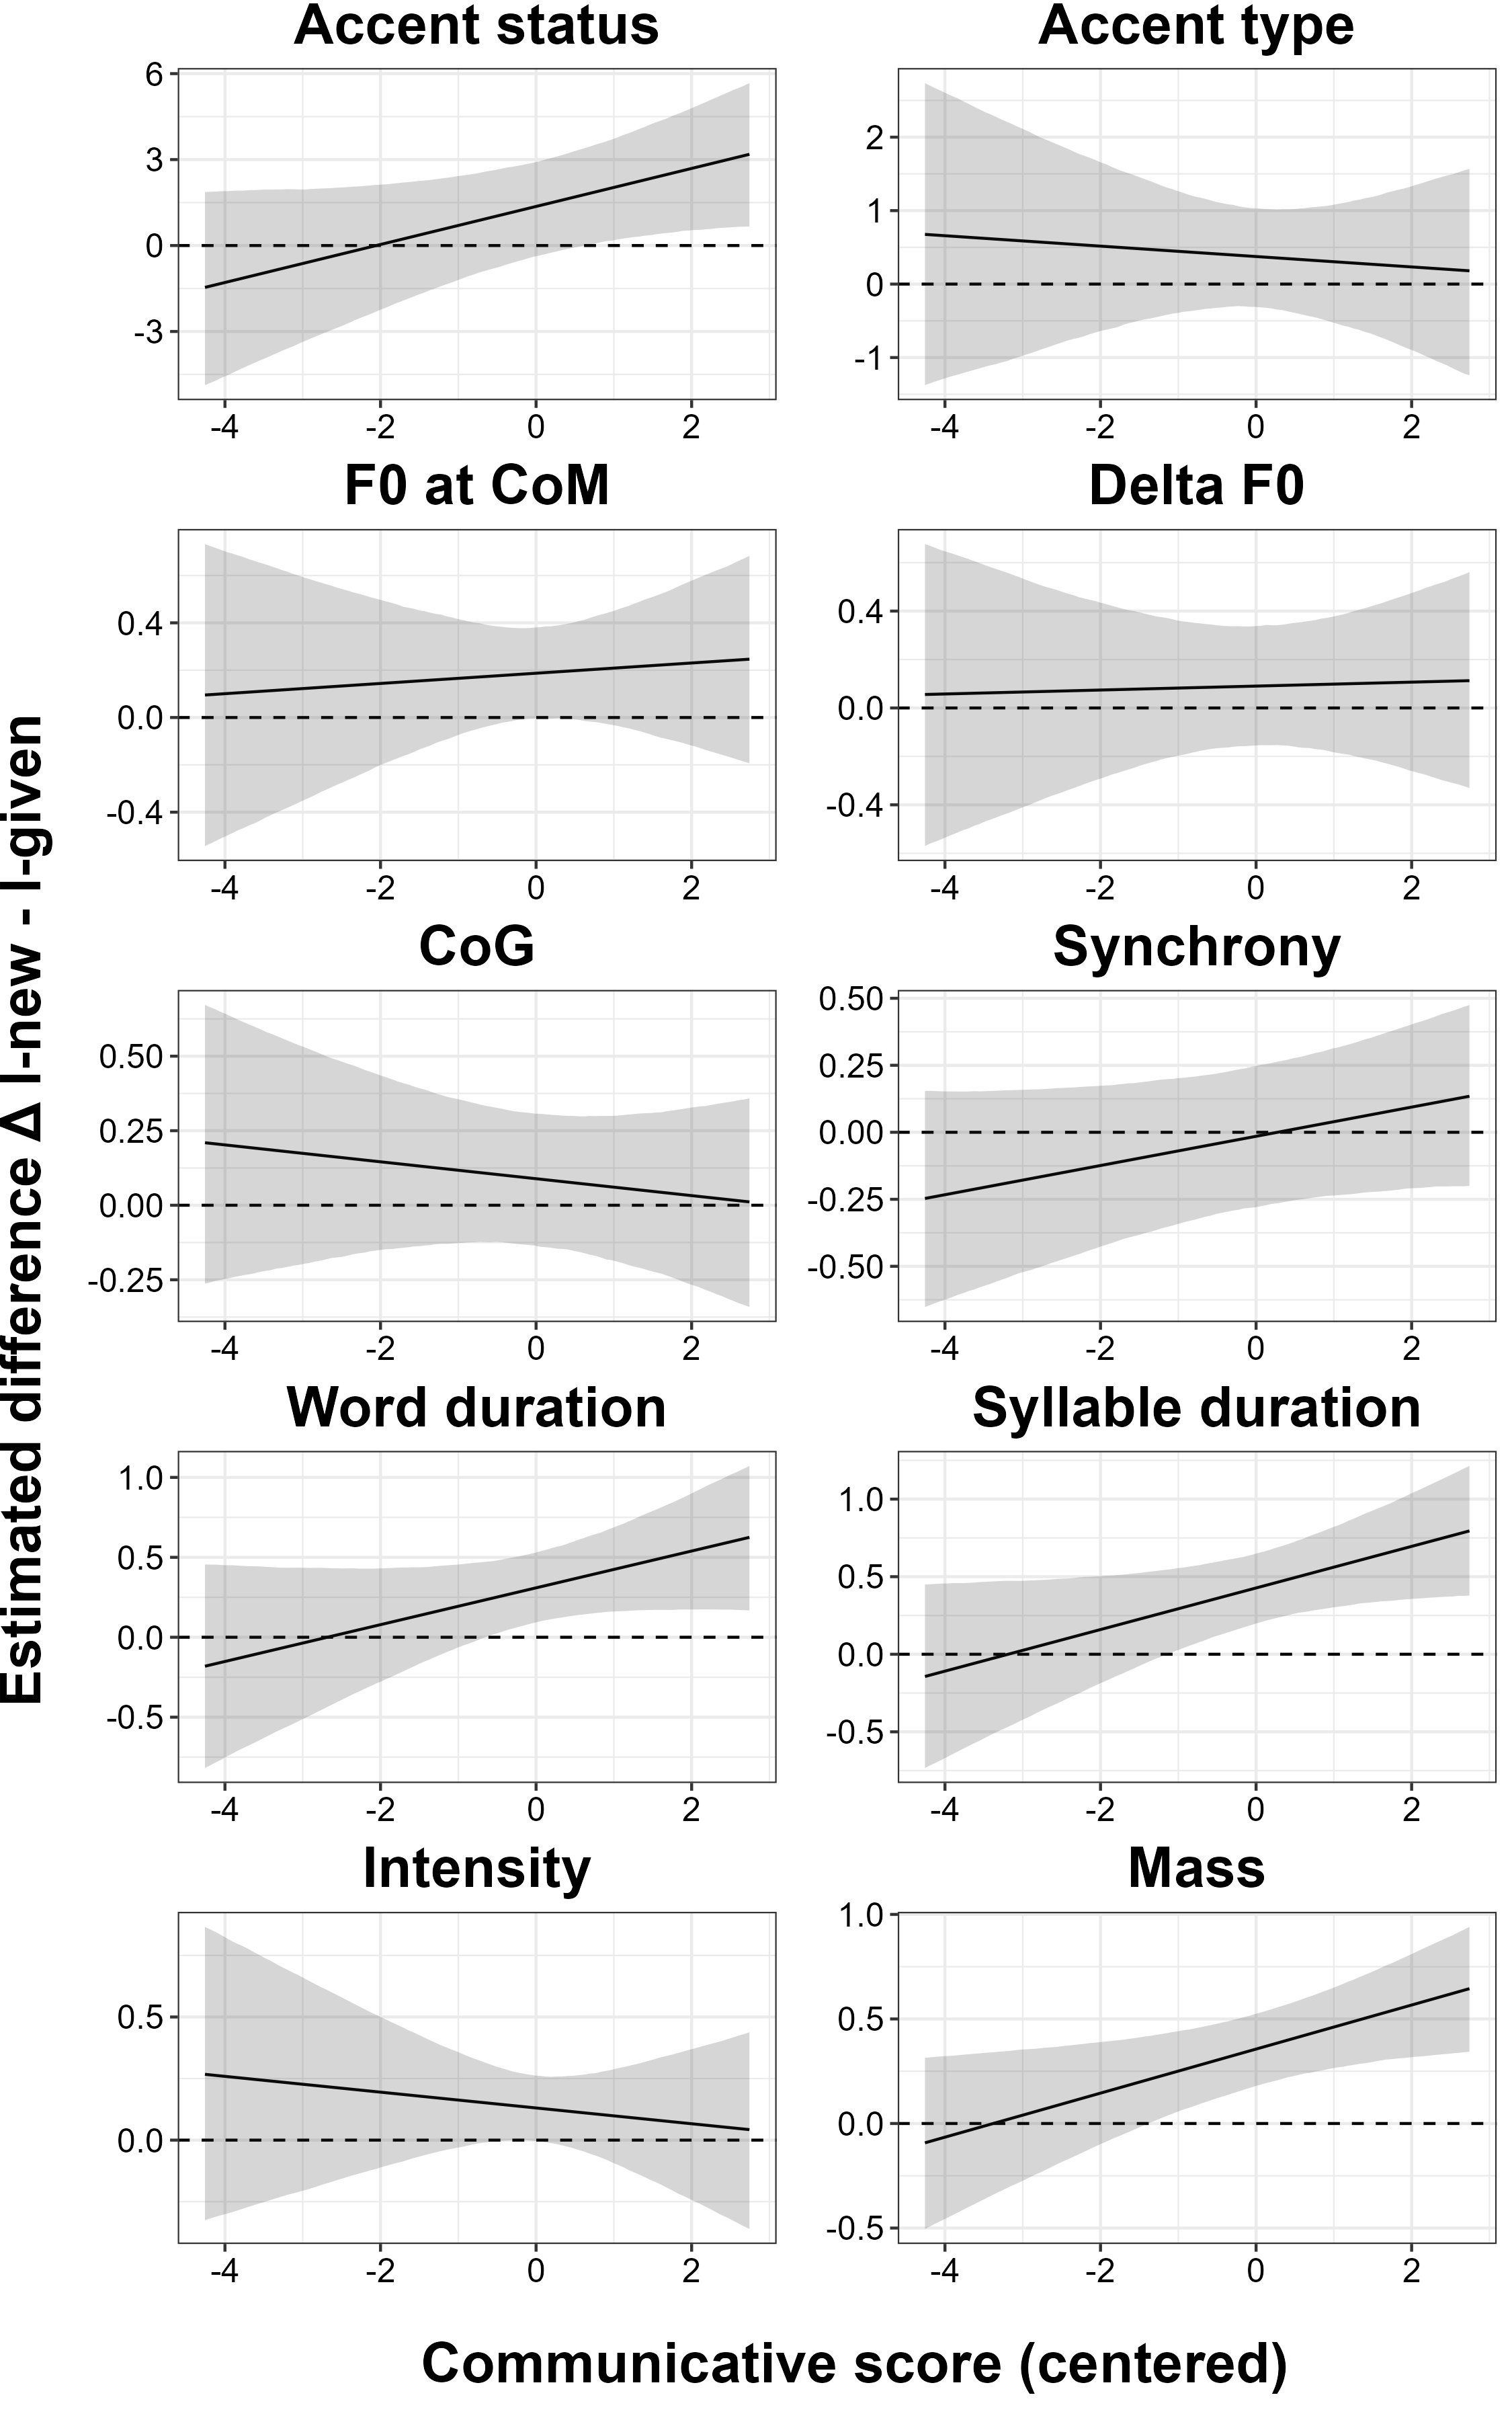
\includegraphics[scale = 0.45]{interactions_lexical-givenness}
	\caption{Estimated differences between lexically new and given referents and 90\% CrIs as a function of communicative score for all parameters.}
	\label{fig:interactions_lexical-givenness}
\end{figure}

Figure \ref{fig:interactions_lexical-givenness} shows the estimated differences between l-new and l-given referents and 90\% CrIs as a function of communicative skill for accent status, accent type, and all eight continuous prosodic parameters. In four parameters (i.e., accent status, word duration, syllable duration, and periodic energy mass), the difference between l-new and l-given referents clearly increases with higher communicative skill to the extent that only speakers with higher communicative skill appear to reliably mark a difference between them. That is, speakers who rated themselves as more communicatively skilled used these parameters more effectively in the expected direction to encode a difference in lexical givenness than speakers with lower communicative skill. The same is true for synchrony, which shows a clearly positive slope, however, the 90\% CrIs include zero for all values of communicative skill. While for F0 at CoM and Delta F0, there barely seems to be a positive moderating effect of communicative skill on the encoding of lexical givenness, accent type, CoG and intensity show a slight decrease in the difference between l-new and l-given with higher communicative skill. However, for all of these latter five parameters, the CrIs include zero for all values of the communicative score variable as can be seen in Figure \ref{fig:interactions_lexical-givenness}. It is thus unlikely that any of the speakers use accent type, F0 at CoM, Delta F0, CoG, synchrony or intensity to encode lexical givenness regardless of their communicative skill.

In Figure \ref{fig:interactions_referential-givenness}, the interactions between referential givenness and communicative skill are plotted. Here, we can generally observe the opposite trend to lexical givenness: Speakers identifying as more communicatively skilled make less of a distinction in the expected direction between r-new and r-given referents in six out of the ten prosodic parameters (accent status, accent type, F0 at CoM, Delta F0, intensity, and periodic energy mass). Only in word and syllable duration do we observe the expected positive slope from lower to higher communicative skill. CoG and synchrony also display negative slopes, however here these lead to a larger difference between r-new and r-given referents for communicatively more highly skilled individuals, albeit in an unexpected direction. 

\begin{figure}
		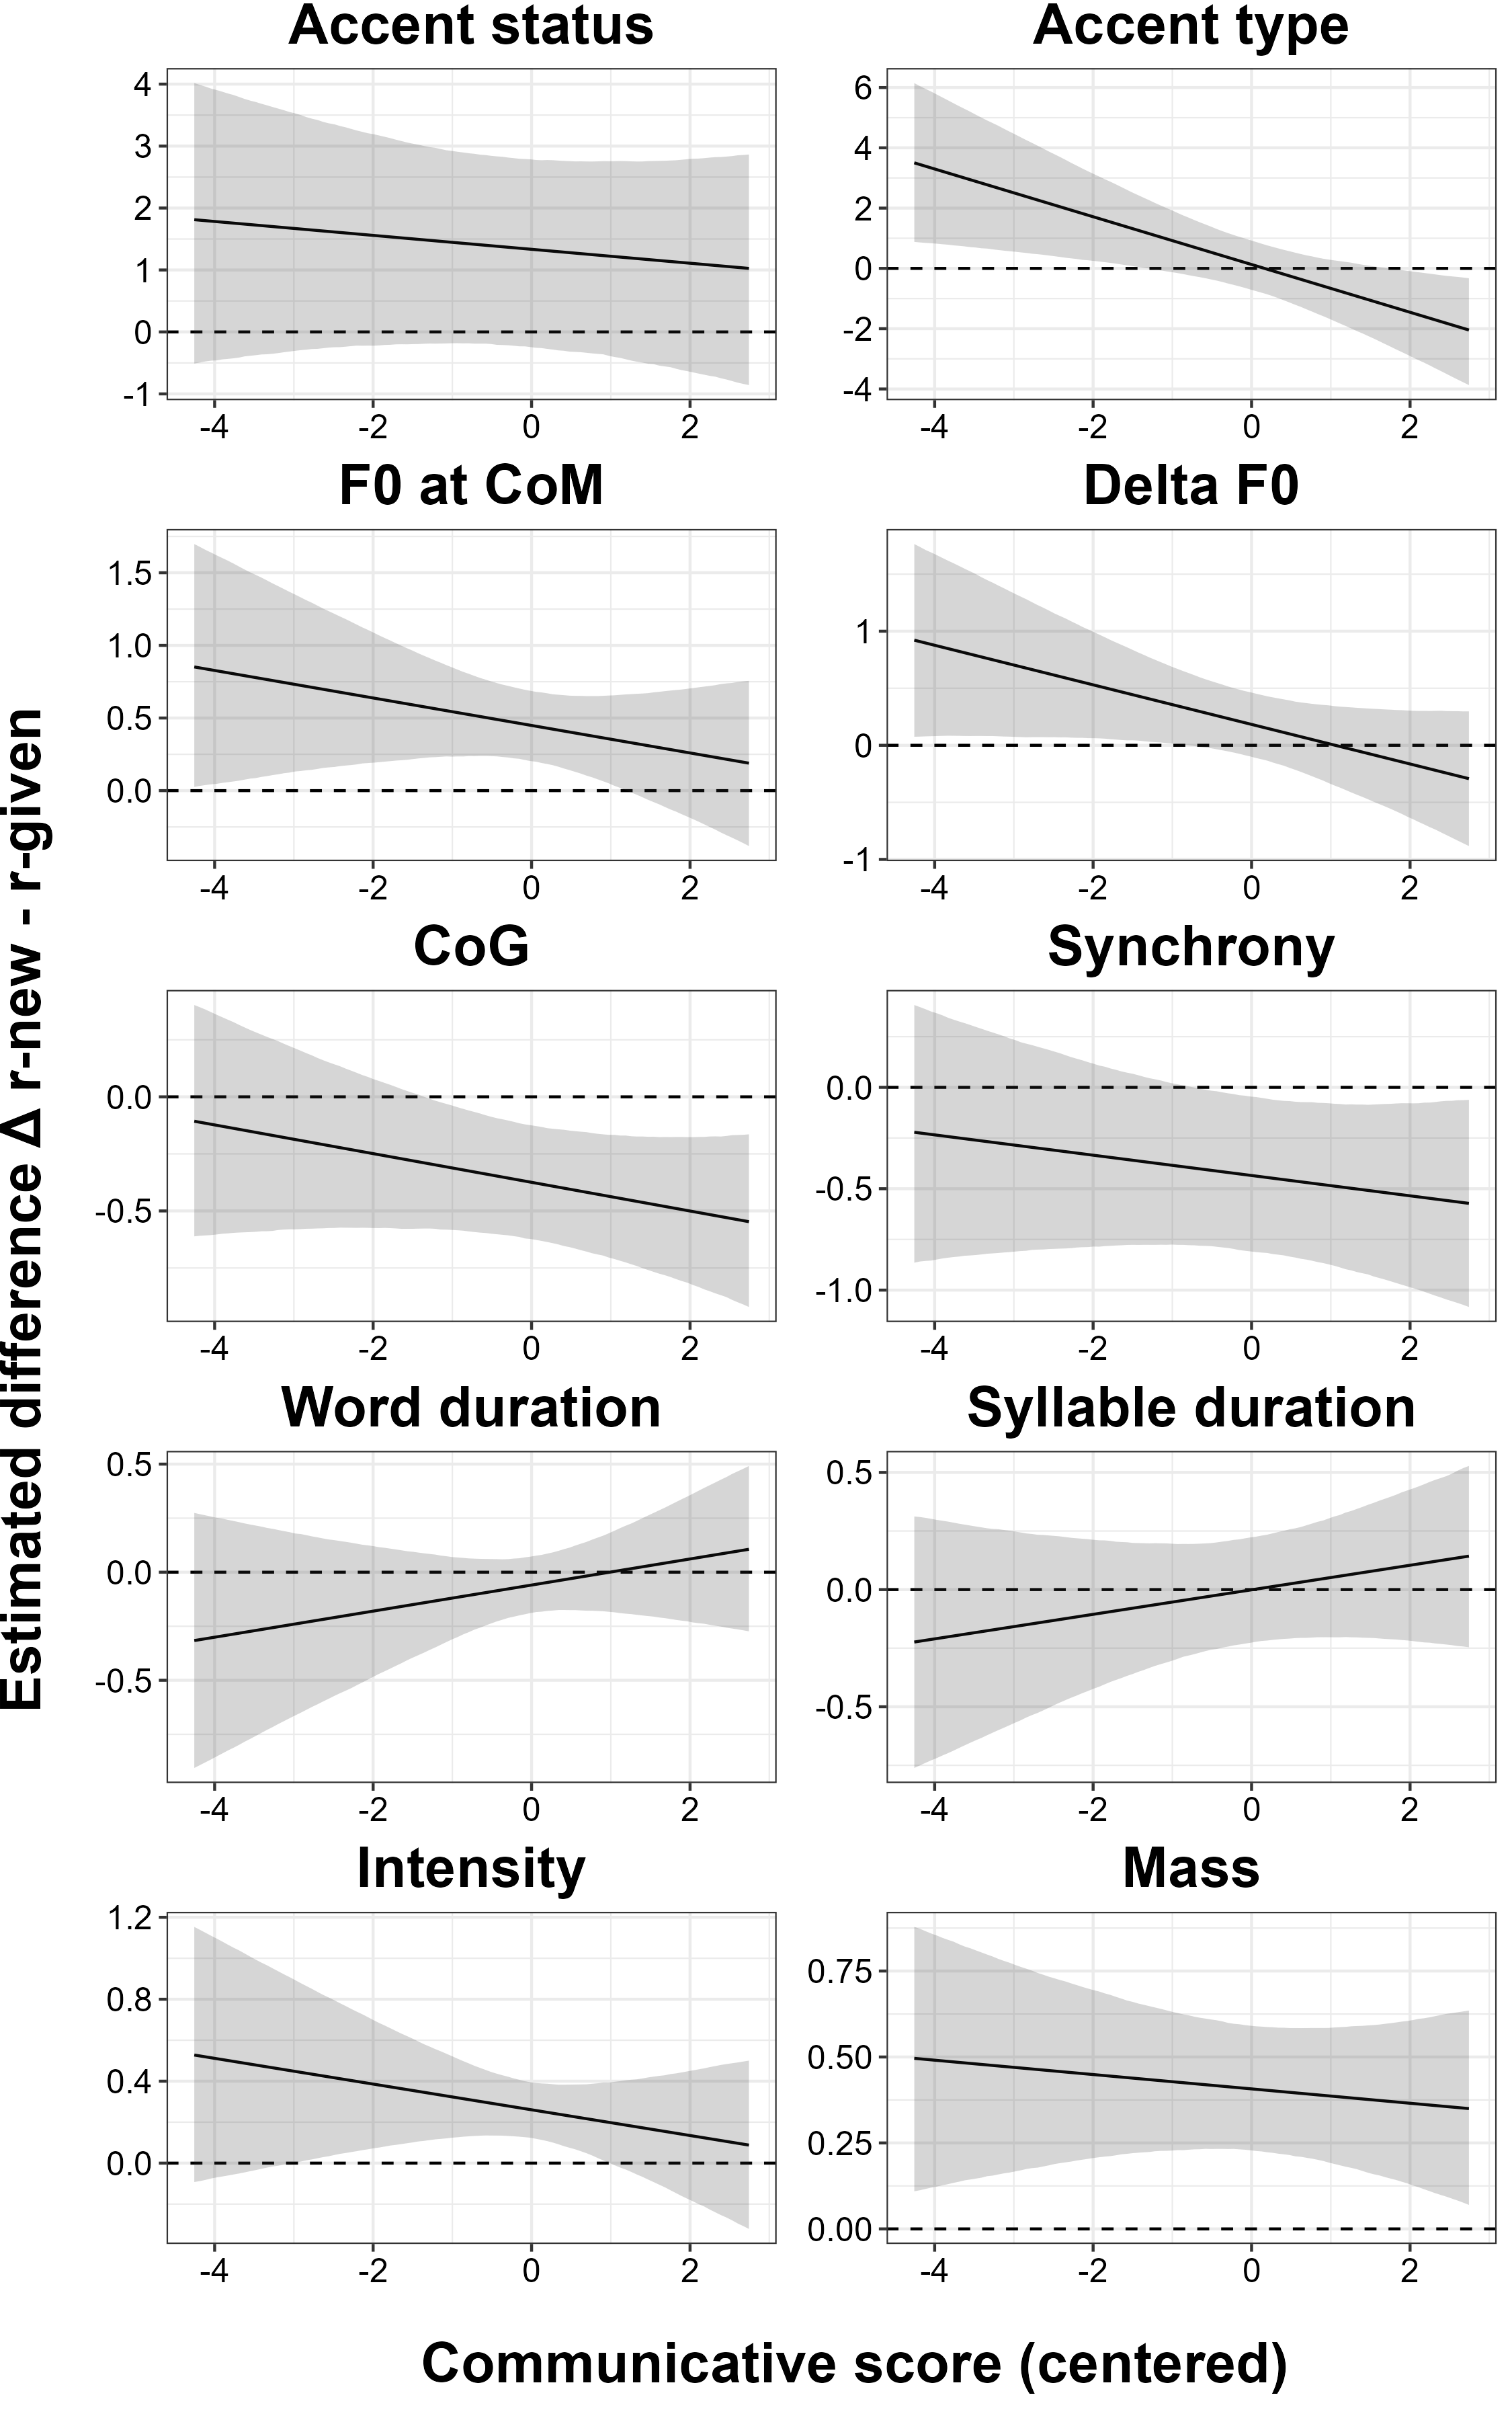
\includegraphics[scale = 0.45]{interactions_referential-givenness}
	\caption{Estimated differences between referentially new and given referents and 90\% CrIs as a function of communicative score for all parameters.}
	\label{fig:interactions_referential-givenness}
\end{figure}

For the encoding of grammatical role, there are again larger positive differences for higher communicative scores in the parameters accent status, word duration, syllable duration, and periodic energy mass and a larger negative difference for CoG (see Figure \ref{fig:interactions_gramm-role}). For the remaining parameters, the moderating effect of communicative skill is relatively subtle as indicated by the flatter slopes in the plots and more extensive overlap between the CrIs and the dashed horizontal zero line. 

\begin{figure}
		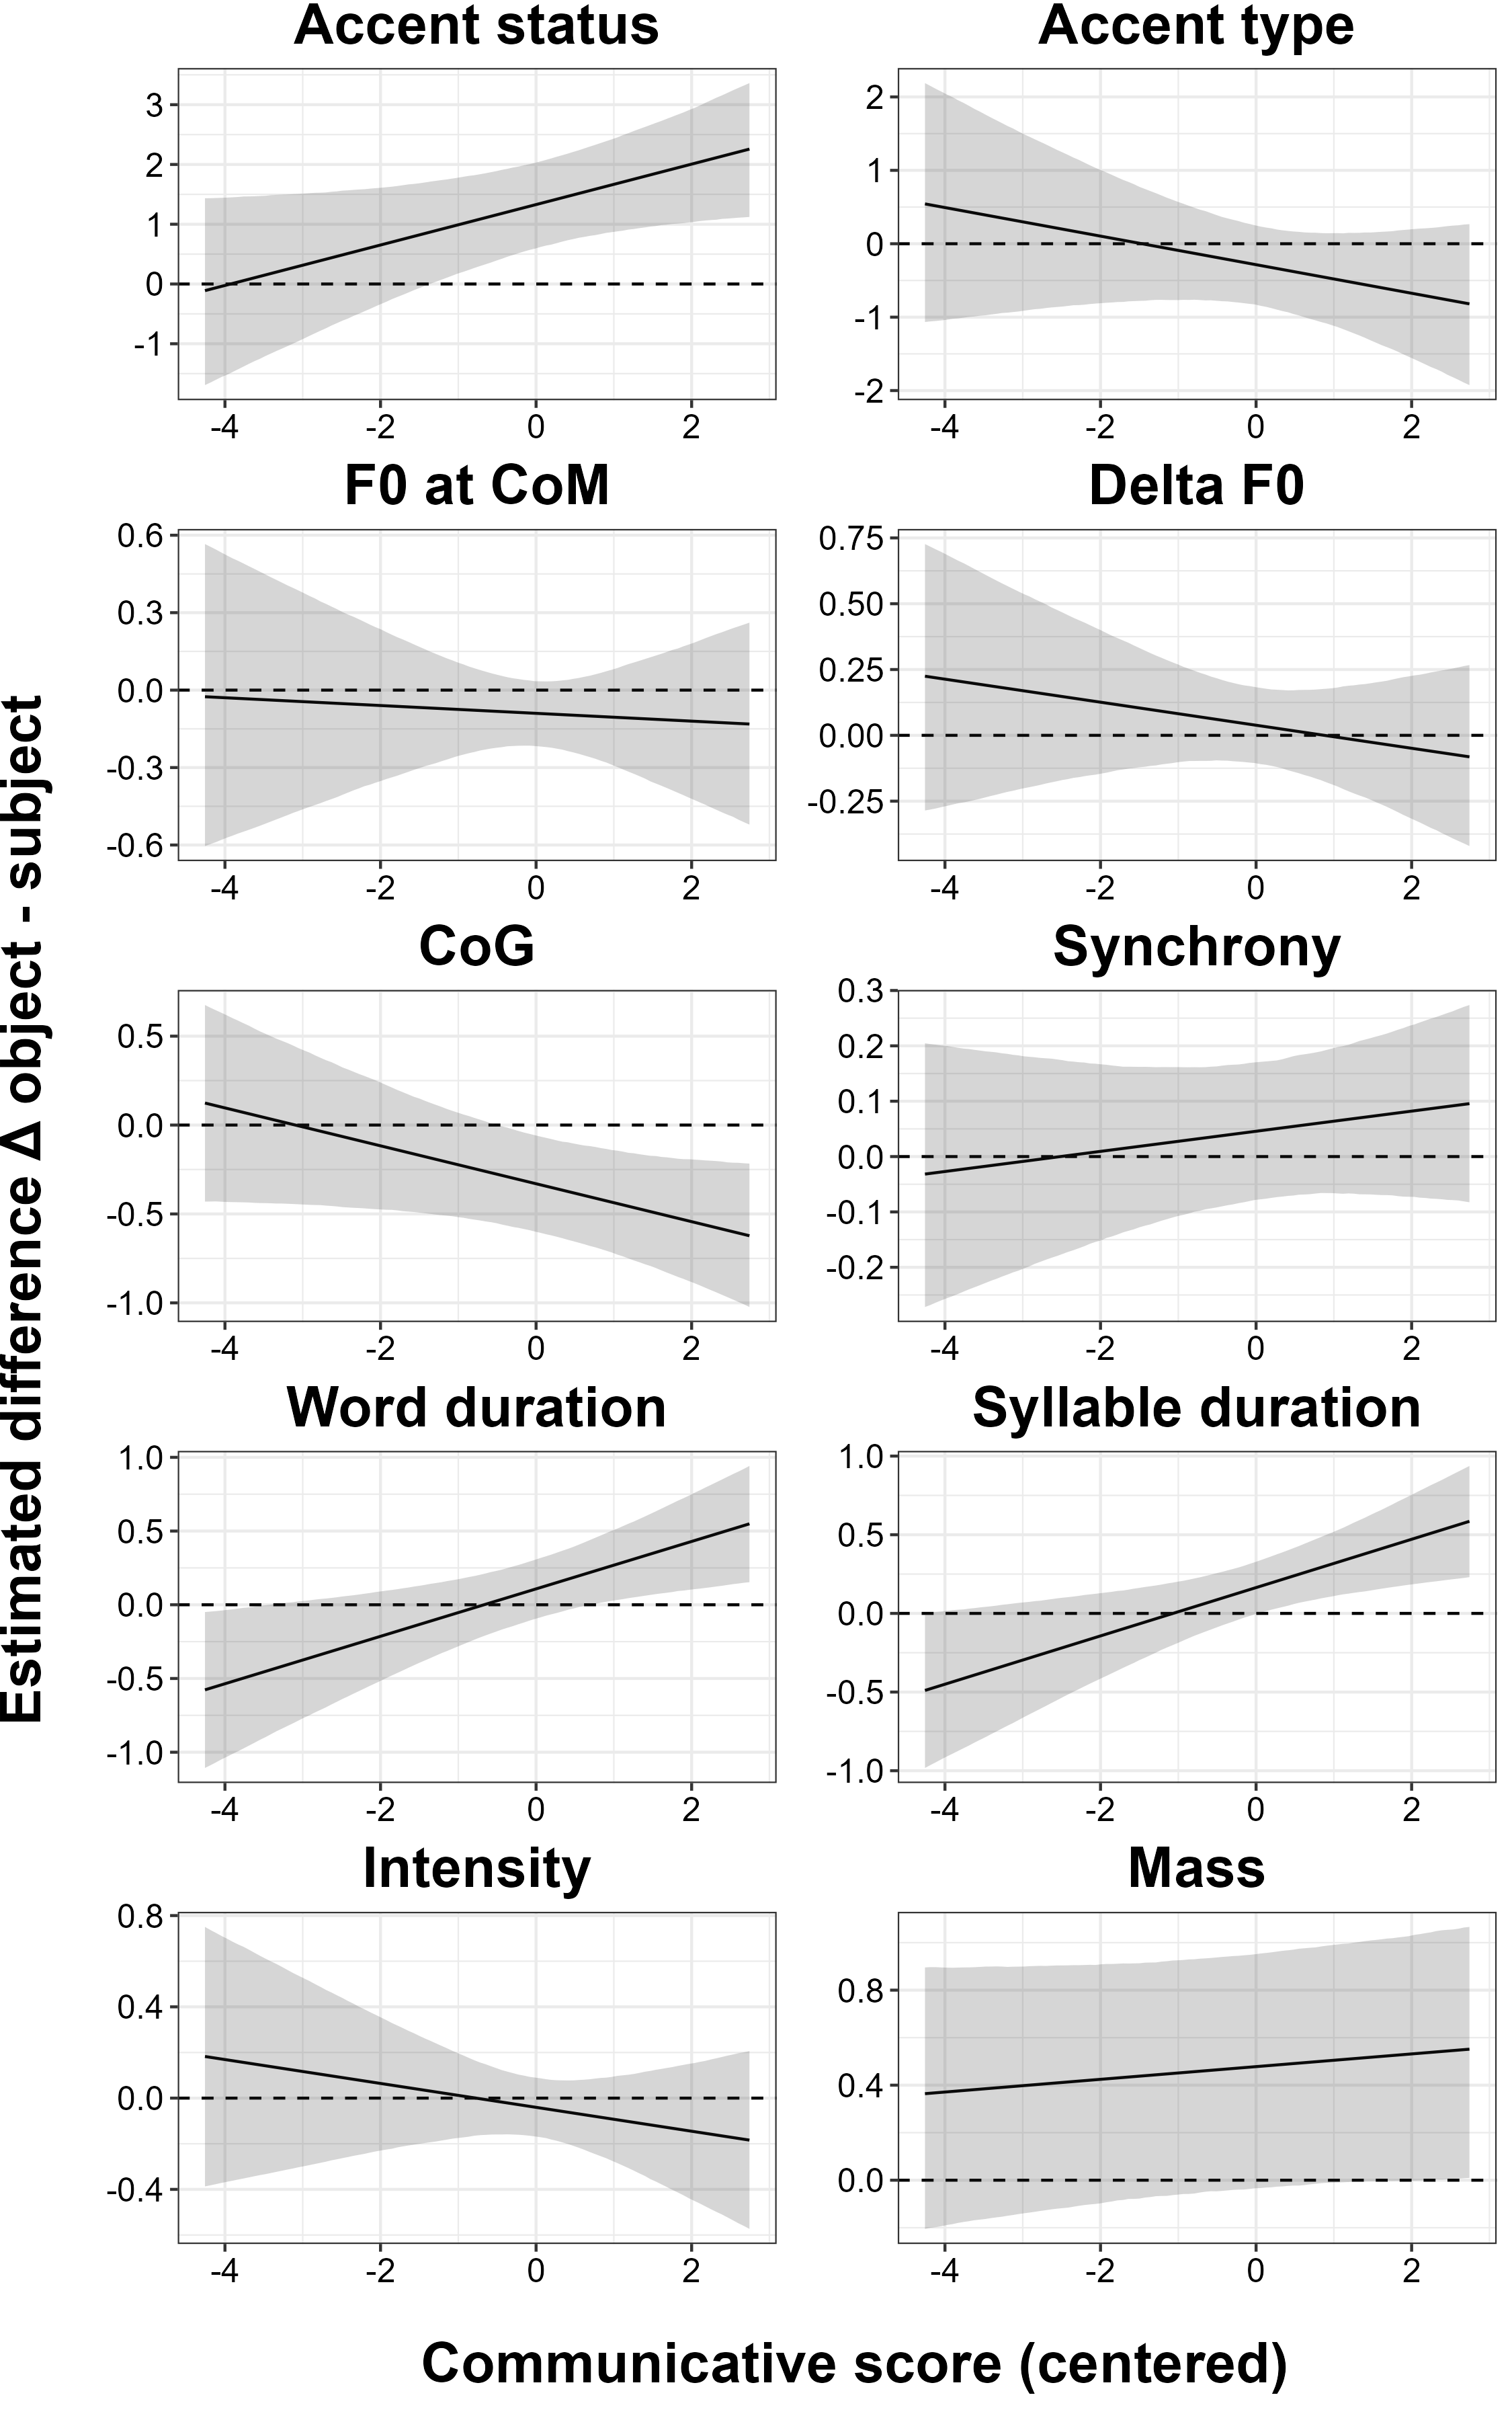
\includegraphics[scale = 0.45]{interactions_grammrole}
	\caption{Estimated differences between grammatical objects and subjects and 90\% CrIs as a function of communicative score for all parameters.}
	\label{fig:interactions_gramm-role}
\end{figure}

Finally, in the encoding of sentence position, differences between initial and medial words are larger for higher communicative scores in F0 at CoM, Delta F0, CoG, synchrony, intensity, and periodic energy mass (see Figure \ref{fig:interactions_position}). For word and syllable duration, this effect is reversed. However, slopes appear to be relatively flat for most prosodic parameters, especially accent status and accent type, with intensity constituting the most notable exception, i.e., the strongest effect of communicative skill. 

\begin{figure}
		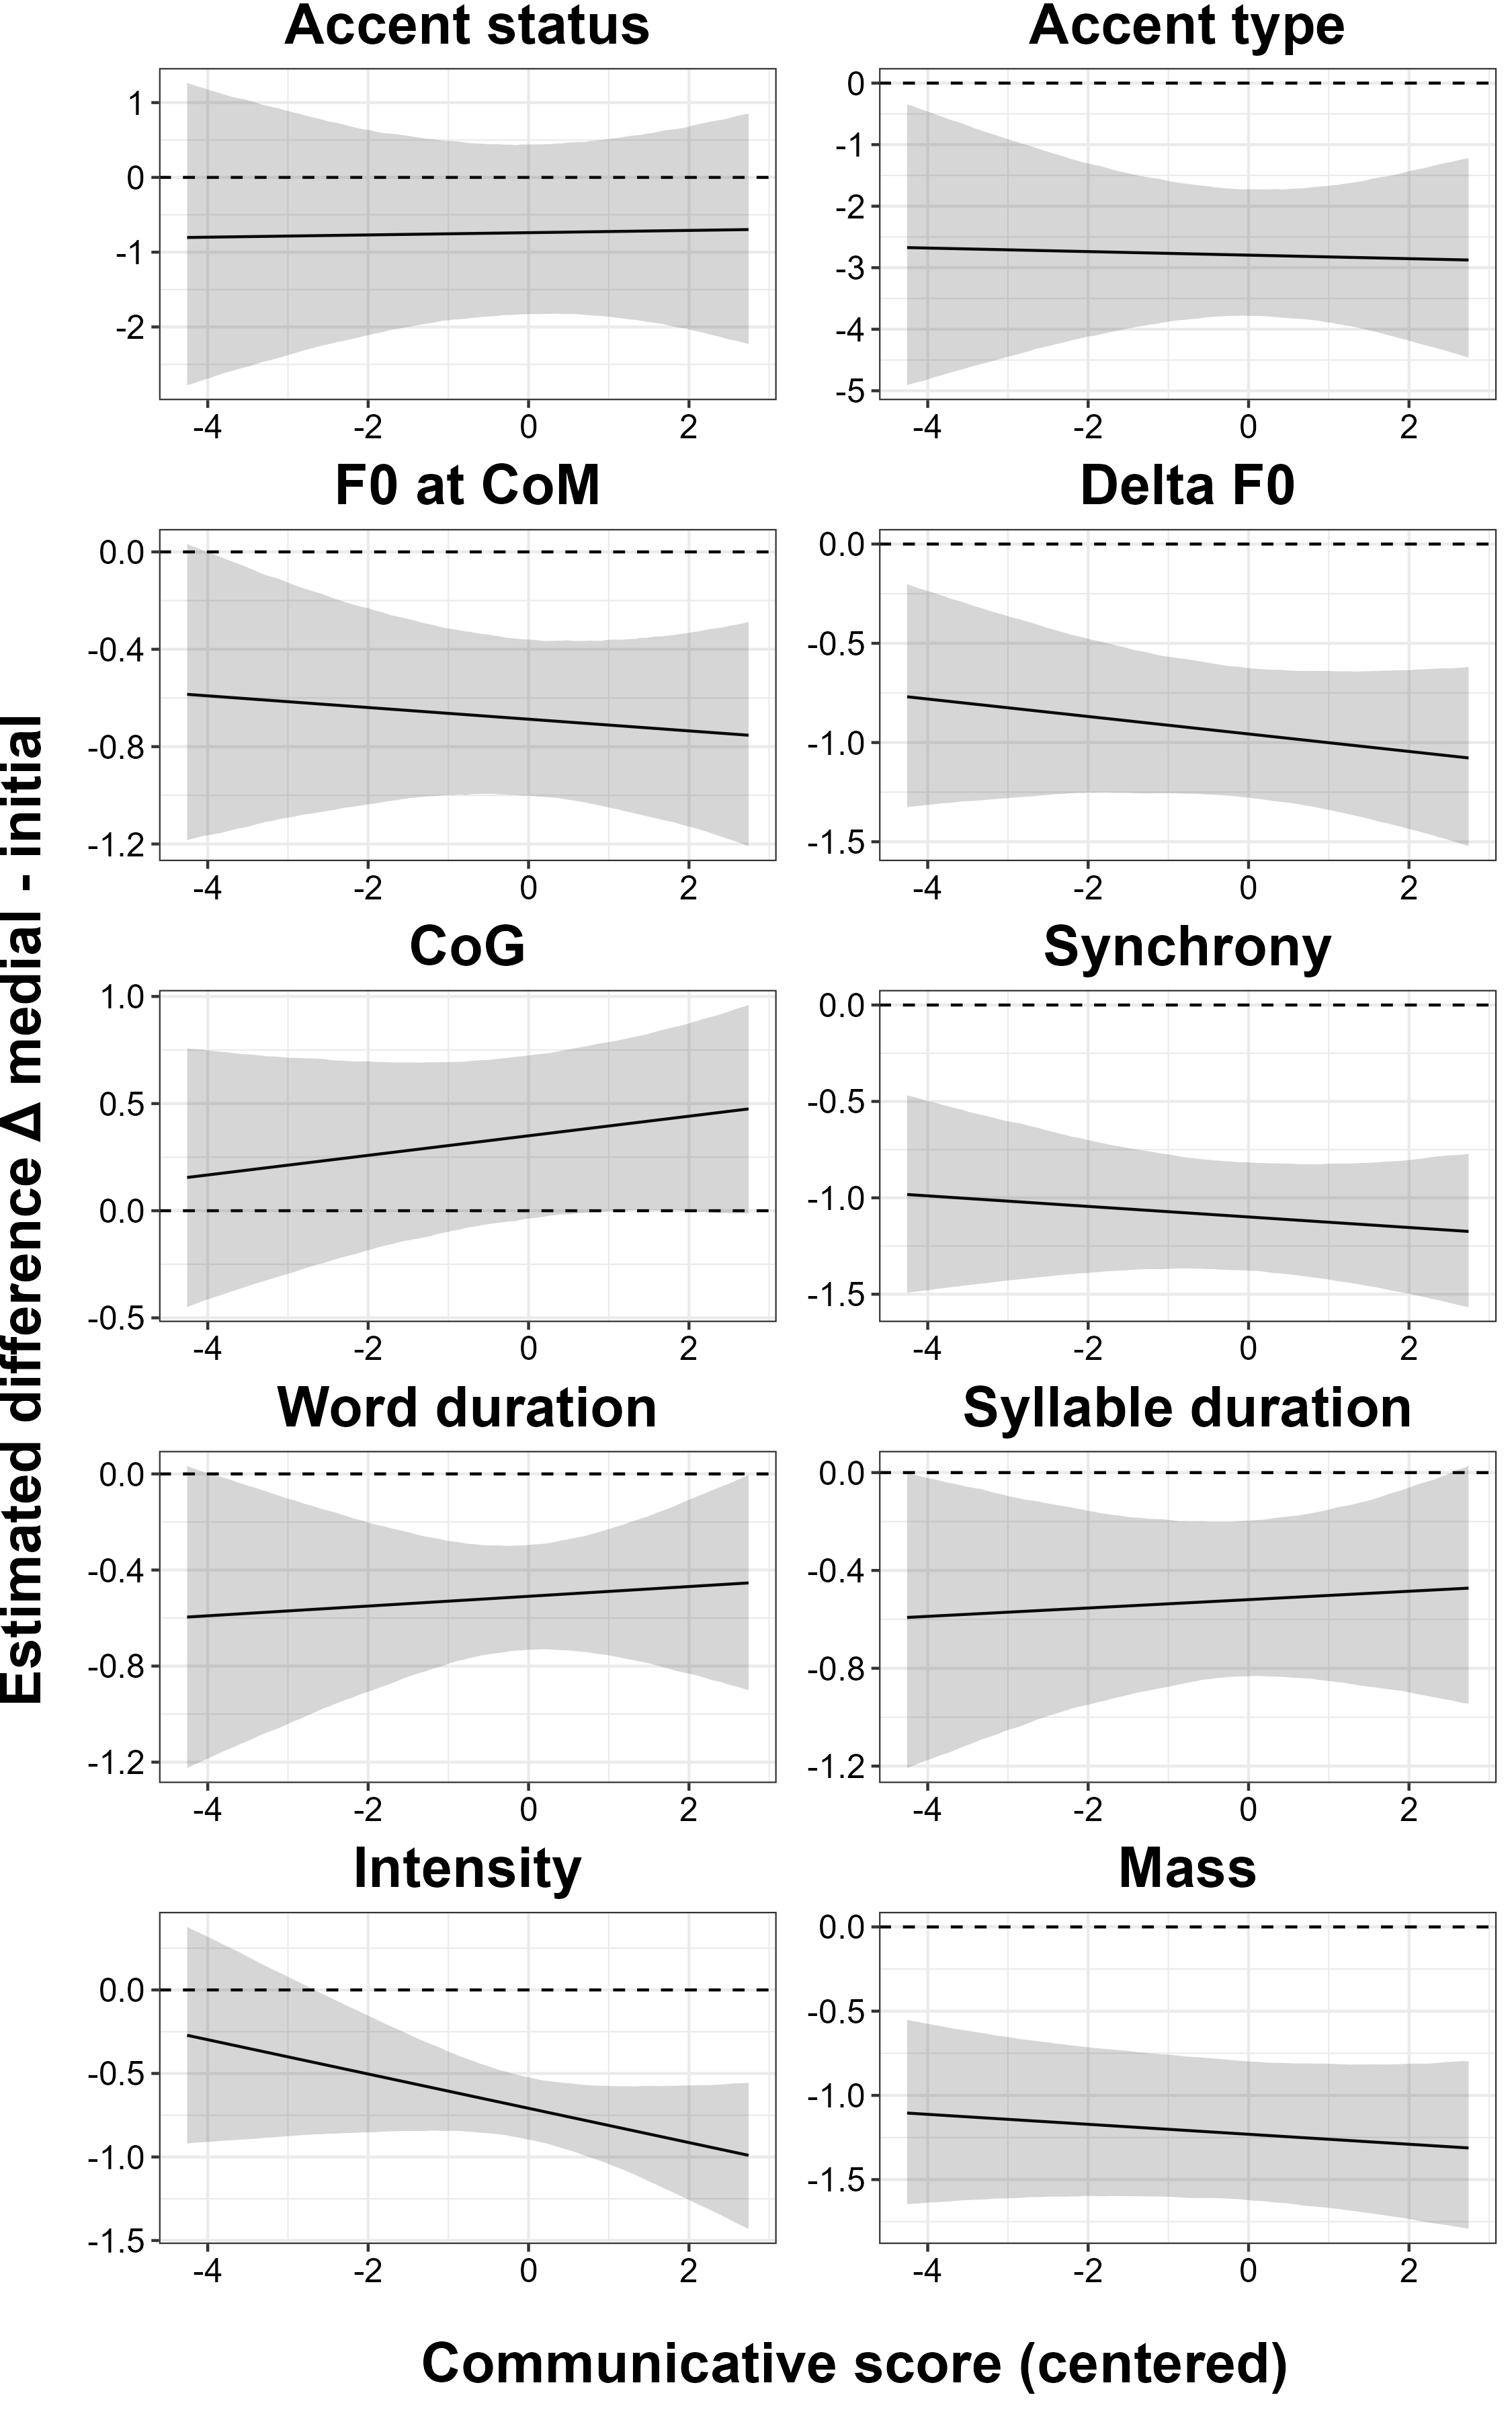
\includegraphics[scale = 0.45]{interactions_position}
	\caption{Estimated differences between words in initial and medial position and 90\% CrIs as a function of communicative score for all parameters.}
	\label{fig:interactions_position}
\end{figure}

\section{Interim discussion} \label{sec:Production2 discussion}

In this study, we investigated the effects of lexical and referential givenness, grammatical role, and sentence position on prosodic prominence production. All four factors were found to influence prominence across speakers. The strongest effect was observed for sentence position, with initial constituents in an utterance generally being produced more prominently than medial target words, more specifically, with more prominent pitch accent types, higher and more steeply rising F0, longer duration, and higher intensity. This result reinforces the importance of an utterance-initial accent in contributing to a rhythmical frame \citep{baumannInfluenceInformativenessProsody2021} and is consistent with Bolinger's (\citeyear{bolingerIntonationItsParts1986}) idea of an \textit{Accent of Power}, which is often placed towards the beginning of an utterance. With regard to information status, our findings confirmed that both the lexical and the referential level influence prosodic prominence \citep{baumannReferentialLexicalGivenness2012, baumannCoreferenceLexicalGivenness2013}. Lexically new as opposed to given target words were reliably marked by longer duration and higher periodic energy mass, but also exhibited strong tendencies to be produced with more nuclear accents and higher F0 and intensity. Referential newness was reliably encoded by higher F0, intensity, and periodic energy mass compared to referential givenness. Finally, grammatical objects were produced with more nuclear accents than subjects, however, the continuous prosodic parameters were least affected by grammatical role out of the four manipulated factors.

On the individual speaker level, we observed different strategies in the prosodic marking of lexical and referential givenness, grammatical role, and sentence position. Of these four factors, the encoding of lexical givenness was least variable in the sense that the cluster analysis revealed only two strategies, which differed only minimally. One cluster encoded the l-new versus l-given contrast slightly more strongly than the other, especially in the prosodic parameters related to timing and intensity. The two strategies we observed for the encoding of referential givenness were more distinct. Here, one cluster relied more on F0 shape and alignment to mark a difference between r-new and r-given referents, while the other cluster used F0 scaling. This observation is reminiscent of a finding by \citet{niebuhrAreThereShapers2011} that German speakers differ in whether they rely more on alignment or scaling to distinguish between different pitch accent types.

Grammatical role was marked less strongly than lexical and referential givenness overall, however, the clustering into three groups appeared to be most stable of all four factors under investigation with the highest average silhouette width. Clusters differed in which cue most reliably encoded grammatical role, with one cluster relying most on CoG and the other two on periodic energy mass. The former cluster additionally made use of periodic energy mass to about the same extent as the other two, leading to a stronger, more redundant encoding of grammatical role in these speakers. These observations show that while averaged group-level results do not reveal any strong tendencies (at least in the continuous parameters), the prosodic productions of individual speakers can be influenced by grammatical role, although this influence manifests in different prosodic parameters. By contrast, sentence position overall was most strongly marked with large differences between initial and medial position for all prosodic parameters and in fact, every single speaker exhibited this trend in at least some of the parameters. Nevertheless, the encoding of sentence position gave rise to the highest number of different strategies as per the cluster analysis. For two clusters, Delta F0 was the most important parameter, for the others it was periodic energy mass. There were also differences in the strength and redundancy of encoding across the clusters, with two of the clusters modifying every parameter. Thus, no matter if the results across speakers indicate a strong overall effect (as for sentence position) or a weak overall effect (as for grammatical role), different speaker-specific strategies may hide under the cover of those general tendencies. To achieve high descriptive adequacy of the relation between prosody and other linguistic dimensions, it is therefore important to consider results below the group level.

To summarize, we found different degrees of variability in the encoding of several semantic-pragmatic and syntactic factors via continuous phonetic parameters. As in the previous production study presented in Chapter \ref{ch:Production I} and similar to previous findings \citep[e.g.,][]{cangemiListenerSpecificPerceptionSpeakerSpecific2015, ouyangIndividualDifferencesProsodic2015, severijnenYourVOORnaamNot2024}, this variability is evident in the strength of encoding of the factors under investigation and the types of parameters used.

With regard to the role of the phonological categories accent status and accent type in the encoding of the different semantic-pragmatic and syntactic factors, we often observed a compensatory behavior at the individual level. Particularly in the marking of referential givenness, grammatical role, and sentence position, speakers using accent status to mark these contrasts were less likely to rely on accent type and vice versa, speakers making use of accent type were less likely to also use accent status. This asymmetry has also been observed in the previously presented production study in Chapter \ref{ch:Production I}. Speakers are thus able to exploit the independency of tune and metrical structure that is postulated by the autosegmental-metrical model \citep[e.g.,][]{laddIntonationalPhonology2008} to encode different linguistic contrasts. This can be regarded as prosodic cue trading not just on a phonetic level as has previously been described by \citet{severijnenYourVOORnaamNot2024} but also on a phonological level. We will return to this point in Chapter \ref{ch: general discussion}.

In this study, deaccentuation of the target word was possible (in the medial position) but rare, only attested in five speakers.\footnote{Deaccentuation may be more frequent in the data than these results suggest, but the difference between a prenuclear accent and deaccentuation is difficult to identify for annotators, especially in this position.} What may ultimately be more important for the information-structural interpretation of utterances than accentuation versus deaccentuation is the structural prominence \textit{relation} between two constituents \citep[e.g.,][]{libermanIntonationalSystemEnglish1975, laddIntonationalPhonology2008, laddProsodicProminenceLanguages2023}. This is particularly relevant for referential givenness, where accent status was more consistently used as a prominence cue across speakers than for lexical givenness. In utterances with referentially new target words, the target word and following verb typically formed a strong-weak pattern, with the target word receiving a nuclear accent and the verb being deaccented. When the target word was referentially given, the pattern was reversed to weak-strong, with the verb receiving the nuclear accent (see also analysis in \citealt{baumannBoostingInhibitingHow2024}). The \textit{weak} target word may either be deaccented or receive a prenuclear accent, but in both cases, the strength relation remained the same. In fact, out of the five speakers that produced deaccented target words, three were among the least consistent users of accent status as a cue to referential givenness.

One reason for the manifestation of different individual strategies that has been considered especially in prominence perception studies is communicative skill. Generally, listeners with higher communicative skill have been found to be more adept at perceiving prominence differences than listeners with lower communicative skill \citep{bishopPhonologyPhoneticsSignalextrinsic2020, orricoInfluenceEmpathyAutisticlike2023}. Analogously, we expected speakers with higher commmunicative skill to encode semantic-pragmatic and syntactic contrasts more strongly than speakers with lower communicative skill. In our data, we observed this expected mediating effect (on several prosodic parameters) for lexical givenness, grammatical role, and sentence position. However, referential givenness seemed to be encoded more clearly by speakers with lower communicative skill, which is contrary to our expectations and the findings by \citet{bishopPhonologyPhoneticsSignalextrinsic2020} and \citet{orricoInfluenceEmpathyAutisticlike2023}. 

That individual speakers should behave differently in their encoding of lexical givenness on the one hand and referential givenness on the other hand may be due to the different sources of these two variables. Referential givenness describes the relation between entities (i.e., creatures, things, states or events) in the situational or textual discourse context, while lexical givenness is determined by the previous occurrence or absence of a word or concept \citep{baumannCoreferenceLexicalGivenness2013}. In fact, our findings are partially in line with Turnbull's (\citeyear{turnbullListenerorientedPhoneticReduction2019}), who found that speakers with lower communicative skill encoded semantic-pragmatic predictability more strongly prosodically than speakers with higher communicative skill. Semantic-pragmatic predictability is comparable to referential givenness in our study. However, \citet{turnbullListenerorientedPhoneticReduction2019} found no mediating effects of communicative skill on the encoding of second mention reduction, which may be claimed to fall within the scope of lexical givenness.
 
The interaction of communicative skill and referential givenness is unexpected in the context of previous perception studies that report a higher sensitivity to the mapping of prosody to meaning in communicatively more skilled listeners \citep{bishopPhonologyPhoneticsSignalextrinsic2020, orricoInfluenceEmpathyAutisticlike2023}. In line with these findings, we assumed that highly communicatively skilled speakers should be able to anticipate the higher activation cost demanded of the listener by an r-new referent \citep{chafeDiscourseConsciousnessTime1994} and thus produce a stronger prosodic contrast to clearly mark the distinction between r-new and r-given. It appears that instead, such speakers underestimated this activation cost and generally produced a weaker contrast. A potential explanation is that the communicatively skilled speakers relied more on the morphosyntactic marking of r-givenness, since r-new referents were preceded by an indefinite article, while r-given referents were preceded by a definite article, making an additional prosodic marking obsolete. 

Like \citet{turnbullListenerorientedPhoneticReduction2019}, we also observed inconsistent mediating effects of communicative skill on different prosodic parameters. However, these inconsistencies were at least partially systematic: For lexical givenness and grammatical role, prosodic variables related to timing, such as accent status, word and syllable duration, and periodic energy mass, were most affected by communicative skill. For referential givenness, the parameters describing the alignment and scaling of the F0 contour (i.e., accent type, F0 at CoM, Delta F0, CoG, and synchrony) were modulated to a larger extent by communicative skill. Nevertheless, it remains unclear at this point why communicative skill should mediate the use of timing but not F0 in the case of lexical givenness and F0 but not timing in the case of referential givenness. This remains an issue for further investigation in future studies.

Our findings are limited by the measure of communicative skill we employed, which is very coarse-grained as it relies on the self-assessment of the participants. Other instruments assessing different aspects of communicative skill could yield more precise results that better relate to speech production in general and the different dimensions of givenness in particular. For example, \citet{orricoInfluenceEmpathyAutisticlike2023} employed a questionnaire to measure emotional and cognitive empathy \citep{baron-cohenEmpathyQuotientInvestigation2004} and found that empathy affects the processing of contrastive focus. Furthermore, we considered relatively few participants (especially compared to perception studies), and most of them had high communicative skill, which limits the generalizability of our findings. 

Previous studies investigating individual variability often only looked at one factor to be encoded prosodically at a time, e.g., focus type in \citet{cangemiListenerSpecificPerceptionSpeakerSpecific2015}. This study finds that some speakers are more successful at distinguishing between focus types than others. A reasonable deduction could thus be made that there are ``good" and ``bad" communicators, i.e., speakers who more or less effectively use prosody to encode meaning. By considering several semantic-pragmatic and syntactic factors to be encoded by prosody in the same study, we contribute more insight to the idea of strong versus weak encoders. In particular, this study shows that speakers who strongly mark lexical givenness prosodically are not at the same time the stronger encoders of referential givenness (and grammatical role and sentence position). In the interactions with communicative skill, it is evident that the encoding of lexical and referential givenness may require different skills or traits of speakers. However, to lend more insight into individual variability and its impact on communicative success, a perception study is needed to disentangle the effects of semantic-pragmatic, syntactic, and prosodic cues on the interpretation of prominence. This is the main objective of the next Chapter. 

\chapter{Perception: Individual variability in the decoding of multiple prosodic and non-prosodic cues to prominence}
\label{ch: Perception}
\chaptermark{Perception study}

\section{Overview}

This chapter presents the findings of a perception study to complement the two production studies discussed in the preceding chapters. We conducted a prominence rating task on visual analogue scales to probe the effects of multiple prosodic (categorical and continuous), syntactic, and semantic-pragmatic cues on the perception of prominence in German listeners. Recordings collected as part of the study presented in Chapter \ref{ch:Production II} were used as stimuli. At the individual level, we will explore how and to what extent listeners differ in their response to these different prominence cues.

Prominence perception is influenced by a variety of factors related to several linguistic levels (see Chapter \ref{ch:background prominence}). Beside prosody, lexical factors (e.g., word frequency and part-of-speech) have been found to play a role for the perception of prominence in German in previous studies \citep[e.g.,][]{baumannWhatMakesWord2018, wagnerExploitingSpeechgestureLink2019}. What is more, listeners may respond to different cues in their decoding of prominence. For example, \citet{baumannWhatMakesWord2018} found that some listeners paid more attention to prosodic variables, especially those related to the F0 contour, while other listeners relied more on lexical and semantic-syntactic factors, such as lexical frequency, part-of-speech, and the presence or absence of a focus particle. Similarly, \citet{wagnerExploitingSpeechgestureLink2019} observed that some listeners relied more on prosodic cues, such as duration, intensity, and F0 changes, and others more on structural cues, e.g., part-of-speech and stressability, in their prominence perception. \citet{orricoInfluenceEmpathyAutisticlike2023}, testing the effects of accent type (H* versus L+H*) and contrastiveness on the perception of prominence in British English participants, found some listeners to be guided more by phonetics (i.e., accent type) and others by pragmatics (i.e., contrastiveness). However, these studies did not consider discourse context, only presenting isolated sentences in their prominence rating tasks. We plan on expanding on this line of research by considering multiple prosodic and non-prosodic variables in a prominence rating task. By presenting stimuli in context, we are able to consider nuanced discourse meaning in the form of lexical and referential information status. A similar study has previously been conducted by \citet{coleSignalbasedExpectationbasedFactors2010}, who presented longer stretches of speech in an RPT task in American English and investigated repetition as a potential predictor of prominence, among other cues. Nevertheless, our approach to discourse meaning is more differentiated and our main objective is to investigate individual differences in the effects of these factors on the perception of prominence. In addition, we consider syntactic factors, i.e., grammatical role and position in the sentence, which adds another linguistic layer that has previously received less attention in prominence perception studies. Syntactic structure is known to interact with prosodic structure (see Section \ref{section: lexical and syntactic}) and it has been shown that individual speakers differ in their mapping of the two domains \citep{huttenlauchIndividualVariabilityProsodic2022}. Considering these two classes of non-prosodic factors in addition to several categorical and continuous prosodic variables will thus lend new insights with regard to individual listener preferences or similarities in the perception of prominence.

In the weighting of these variables, we expect categorical prosodic cues, such as accent status and accent type, to play a particularly important role for prominence perception as previous studies on West-Germanic languages have already demonstrated \citep[e.g.,][]{baumannWhatMakesWord2018, wagnerExploitingSpeechgestureLink2019, bishopPhonologyPhoneticsSignalextrinsic2020}. However, listeners may differ in their weighting of the available cues, some potentially being driven more by prosodic and others by non-prosodic cues. As in the previously presented production study (see Chapter \ref{ch:Production II}), we collected information on participants' communicative skill as a possible explanation for such differences in behavior. In line with prior observations \citep[e.g.,][]{bishopPhonologyPhoneticsSignalextrinsic2020, orricoInfluenceEmpathyAutisticlike2023}, we expect listeners with higher communicative skill to be more sensitive to prosodic prominence cues. 

The results of the present study confirm that most prosodic parameters affect prominence ratings in an expectable way: Higher values in the continuous prosodic parameters generally result in higher prominence ratings, words with a nuclear accent are perceived as more prominent than prenuclear accented and deaccented words and the hierarchy of perceived prominence of pitch accent types largely confirms previous findings \citep[e.g.,][]{baumannPerceptualProminencePitch2015}. Among the prosodic variables, accent status, word duration, and accent type are the most important predictors of prominence, while the non-prosodic cues play only a subordinate role. Across listeners, there are only subtle differences in the sensitivity to and weighting of cues. One group of listeners is more strongly affected by all cues, prosodic and non-prosodic, in their prominence ratings, weighting accent status and accent type most highly, while the other group is less sensitive to all cues and guided most strongly by accent status and word duration. Evidence for an effect of communicative skill is weak.

The remainder of this chapter is structured as follows: In Section \ref{sec:s3_methods}, we describe the stimuli, data collection procedure, and participants as well as the statistical methods used in the analysis. Section \ref{sec:s3_results} presents the results of the study starting with an overview of the overall results across participants before narrowing in on individual differences and similarities in the observed patterns. Finally, Section \ref{sec:s3_discussion} concludes with an interim discussion of this chapter's findings.

\section{Methods} \label{sec:s3_methods}

\subsection{Stimuli, procedure, and participants}

We conducted a prominence rating task with gradual visual analogue scales (or slider scales) ranging from 0 to 100 implemented online in SoSci Survey \citep{leinerSoSciSurvey2024}. Participants were presented with 47 short excerpts of written text and corresponding audio consisting of three to five sentences. They were asked to rate how highlighted an underlined target word sounded to them after listening to the whole excerpt (see Figure \ref{fig:S3_soscisurvey} for a screenshot of an example task). Participants were allowed to listen to the excerpts as many times as they liked. The 47 target items were preceded and followed by five items sampled from different stories, which did not enter the analysis, to serve as practice items and to counteract potential effects of declining attention. After the completion of the prominence rating task, participants were asked to provide basic sociodemographic information and fill out a short questionnaire on their communicative skill. The whole procedure took on average 20 minutes.

\begin{figure}[t]
		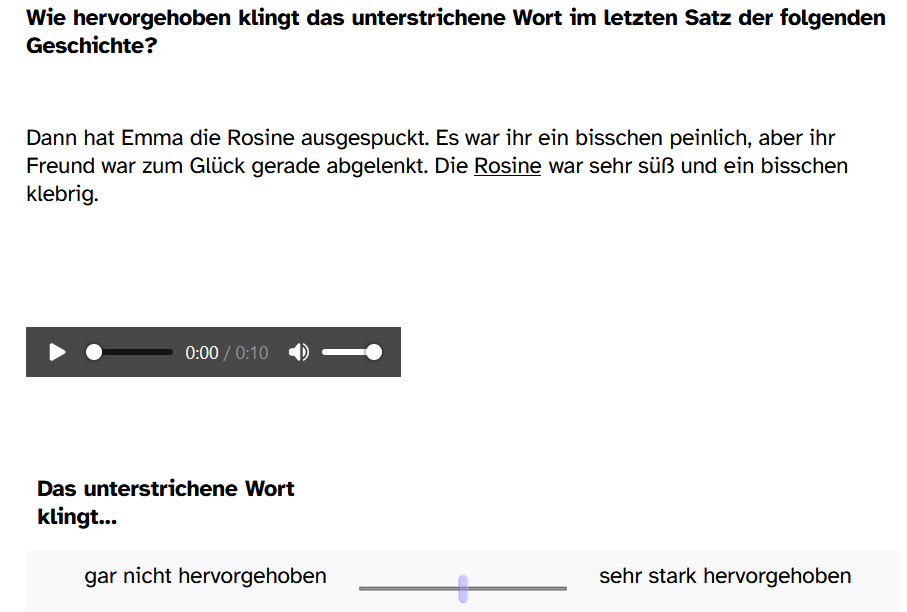
\includegraphics[width=\textwidth]{S3_soscisurvey}
	\caption{Example screen of the prominence rating task implemented in SoSci Survey.}
	\label{fig:S3_soscisurvey}
\end{figure}

Excerpts were sampled from eight different coherent stories, namely the stories recorded in the production study presented in Chapter \ref{ch:Production II}. We selected productions from eight different speakers (three male, five female). Target words were always nouns and appeared in the last sentence of the excerpt but differed in whether they occurred in medial or initial position, as an object or subject, as lexically new or given (i.e., previously mentioned in the same excerpt) and as referentially new or given (i.e., referring to a previously introduced entity in the discourse, see also Table \ref{table:summary_manipulations} in Chapter \ref{ch:Production II}). To ensure that sufficient context would be available to listeners to correctly interpret the lexical and referential information status of the target word, each excerpt consisted of the utterances up until and including the previous mention of the same word (see Figure \ref{fig:S3_soscisurvey} for an example). In the case of the lexically new target words (Target 1), we presented the excerpt from the beginning of the story, which did not include another mention of the same word. 

In addition, target words differed in their prosodic realization, representing a wide range of accent types in prenuclear and nuclear position as well as deaccentuation. We also measured several continuous phonetic parameters in the target words, i.e., the same parameters analyzed in the production experiments presented in Chapters \ref{ch:Production I} and \ref{ch:Production II}: F0 at the Center of Mass (F0 at CoM), Delta F0, Center of Gravity (CoG), synchrony, word and syllable duration, intensity, and periodic energy mass. Table \ref{table:s3_stimuli} summarizes the distributions of the stimuli in terms of accent status and accent type. The feature distributions of the stimuli roughly reflect the distributions observed in the production experiment presented in Chapter \ref{ch:Production II}. The loudness of the recordings was normalized to the same target level before they were entered into the experiment. The stimuli were presented in pseudo-randomized order, ensuring that Target 1 of a story always occurred before the remaining target words, so that the item was truly lexically new to the participants.

\begin{table}[]
\begin{tabular}{llllll}
\lsptoprule
Accent status & Target1 & Target2 & Target3 & Target4 & Target5 \\
\midrule
\multirow{7}{*}{Nuclear}    & 2 L+H*           & 1 L+H*           & 2 L+H*           & 1 L+H*           & 2 L+H*           \\
                            &                  &                  & 2 L*+H           &                  & 2 L*+H           \\
                            & 2 H*             & 1 H*             &                  & 1 H*             &                  \\
                            & 2 H+!H*          & 1 H+!H*          &                  & 1 H+!H*          &                  \\
                            & 1 H+L*           & 1 H+L*           &                  & 1 H+L*           &                  \\
                            & 1 !H*            &                  &                  &                  &                  \\
                            &                  &                  &                  & 1 L*             &                  \\
                            \midrule
\multirow{6}{*}{Prenuclear} &                  & 1 L+H*           & 2 L+H*           & 1 L+H*           & 2 L+H*           \\
                            &                  & 1 L*+H           & 2 L*+H           & 1 L*+H           & 2 L*+H           \\
                            &                  & 1 H*             &                  &                  &                  \\
                            &                  & 1 H+L*           &                  &                  &                  \\
                            &                  & 1 !H*            &                  & 1 !H*            &                  \\
                            &                  & 1 L*             &                  & 1 L*             &                  \\
                            \midrule
Deaccented                  &                  & 2                &                  & 2                &                  \\
\midrule
Total number                       & 8                & 12               & 8                & 11               & 8                \\
\lspbottomrule
\end{tabular}
\caption{Distribution of selected stimuli by target word position, accent status, and accent type.}
\label{table:s3_stimuli}
\end{table}

Responses were collected from 65 monolingual native speakers of German (25 female, 39 male, 1 non-binary) between the ages of 18 and 71 years (mean = 32, SD = 9.6). To the best of our knowledge, none of the participants had taken part in either of the two production studies. Each participant contributed 47 prominence ratings for a total of 3,055 data points. Most participants (n = 55) were from Germany, especially North Rhine-Westphalia, Baden-Wuerttemberg, and Lower Saxony, and ten participants were from Austria. The majority of participants (n = 62) reported no prior experience with speech analysis, three participants had basic experience, and no participant reported any hearing impairment. In addition, we collected information on participants' communicative skill using the same questionnaire as in the study presented in Chapter \ref{ch:Production II} (see Section \ref{sec:Production2 methods} and Appendix \ref{Appendix B} for details), i.e., a subset of the Autism Spectrum Quotient \citep{baron-cohenAutismSpectrumQuotientAQ2006}. Communicative scores in our participants ranged from 1 to 10 (possible values: 0-10, where 0 indicates low and 10 high communicative skill), with a mean of 6.4 (SD = 2.0). Participants were recruited via Prolific (\url{https://www.prolific.co/}) and were paid \pounds 5 for the completion of the experiment. 


\subsection{Statistical analysis}

Statistical analyses were conducted in R \citep{rcoreteamLanguageEnvironmentStatistical2022}. For data wrangling and visualization, we used the \pkg{tidyverse} package \citep{wickhamWelcomeTidyverse2019} and \pkg{cowplot} \citep{wilkeCowplotStreamlinedPlot2020} for arranging multiple plots into one. We ran Bayesian regression models using the \pkg{brms} package \citep{burknerBrmsPackageBayesian2017} as an interface to the Stan modeling language \citep{carpenterStanProbabilisticProgramming2017}. To extract posterior estimates from the models, we used the \pkg{tidybayes} package \citep{kayTidybayesTidyData2023}. The random forest analyses were conducted using the \pkg{party} package \citep{hothornUnbiasedRecursivePartitioning2006}. For the cluster analysis, we made use of the \pkg{cluster} package \citep{maechlerClusterClusterAnalysis2022} and \pkg{ggdendro} \citep{devriesGgdendroCreateDendrograms2024} to create the dendrogram.
Data and scripts are available online (\url{https://osf.io/m5xwe/}).

We used zero-one-inflated beta (zoib) regression models, which are appropriate for data generated using visual analogue scales, where values are bounded between zero and one and values at these two end points tend to be relatively frequent, i.e., ``inflated" \citep{liuZoibPackageBayesian2015, vuorreHowAnalyzeVisual2019}. We ran one model per prominence-cueing parameter (i.e., the continuous and categorical prosodic variables and the syntactic and semantic-pragmatic variables) for a total of 14 models, with prominence rating as the dependent variable in each model. We included the prominence-cueing parameter and communicative score as well as their interaction as predictors, random intercepts for listener, word, and speaker, and by-listener random slopes for the prominence-cueing parameter. Zoib models estimate multiple sets of parameters to capture the distributions of ones and zeros as well as the distribution of any values between one and zero, i.e., the beta regression. However, since only 4.6\% of the data are zeros and 3.2\% are ones, we will focus on the results of the beta regression and disregard the parameters capturing zero-one inflation.

The communicative score variable was centered before being entered into the models so that the model parameters are interpretable with regard to the samples' mean. Prominence ratings were scaled within each listener so that the lowest rating for each individual corresponds to 0 and the highest rating to 1. The continuous prosodic parameters were z-scored to make the model estimates comparable across different measuring units (e.g., semitones or decibels). Finally, we collapsed the annotated GToBI accent types into five categories to simplify the corresponding model and make its interpretation more feasible: rising (L+H* and L*+H), high (H* and !H*), falling (H+L* and H+!H*), low (L*), and deaccented.

Models ran for 4,000 iterations on four chains with a warm-up of 2,000 iterations yielding 8,000 posterior samples per model. We specified weakly informative, normally distributed priors with a mean of zero and a standard deviation of one for the regression coefficients and used the default priors supplied by \pkg{brms} for the remaining parameters. Model fits were assessed by ensuring that no model yielded Rhat values larger than one.

As in the previous analyses, we report model results in terms of the regression coefficient $\beta$ and its 90\% credible intervals (CrIs) under the posterior distributions as well as the posterior probability that $\beta$ is larger than zero: Pr($\beta$\textgreater{}0). We consider the effect of a predictor variable to be reliable if the 90\% credible interval (CrI) does not include 0 and the probability that $\beta$ is larger than zero is higher than 0.95 or lower than 0.05.

In order to investigate inter-individual variability in the prominence ratings, we exploit the by-listener random slopes similar to the analyses conducted in Chapters \ref{ch:Production I} and \ref{ch:Production II}. In contrast to the regression models designed for the production studies, the models here all share the same dependent variable (i.e., prominence rating), so that the model estimates including the random slopes are comparable. This allows us to consider categorical and continuous variables together in the same analysis. Since the variables' accent status and accent type are associated with multiple levels and thus multiple random slope estimates, we averaged the random slope values for each of these variables. We ran a cluster analysis on the extracted random slopes following the same procedure as before (see Section \ref{sec: stats study1} for details), which results in a grouping of listeners which are maximally similar within and dissimilar across clusters.

To establish rankings of all variables in terms of their importance for the prominence ratings, we trained random forest models \citep{breimanRandomForests2001}. Random forests have been argued to be particularly suitable for the analysis of multiple predictors, which are potentially collinear and may interact with each other \citep[e.g.,][]{stroblIntroductionRecursivePartitioning2009}. We entered all 14 prosodic and non-prosodic variables as predictors of prominence ratings as the outcome variable into the same model. Models were trained on 70\% of the data and the remaining 30\% of data were used to validate the model by ensuring that the model predictions were correlated with the unseen data. 

\section{Results} \label{sec:s3_results}

\subsection{Overall results}

In this section, we present the results of the regression models used to probe the effects of the prosodic and non-prosodic parameters on prominence ratings across all listeners. Furthermore, we conduct a random forest analysis to rank the variables in terms of their importance in predicting the prominence ratings. These results will serve as a baseline for the analysis at the individual listener level.

Starting with the categorical prosodic variables, Figure \ref{fig:s3_cat_pros_prmtrs} shows the mean predicted prominence ratings and 90\% CrIs for accent status and accent type. As expected, nuclear accented words are perceived as most prominent and deaccented words as least prominent, with prenuclear accented words in between (see Figure \ref{fig:s3_cat_pros_prmtrs}, left). The estimated difference in prominence ratings between prenuclear and nuclear accented words is reliable according to the respective model ($\beta$ = 0.18, CrI = [0.15; 0.20], Pr($\beta$\textgreater{}0) = 1), as are the differences between deaccented and prenuclear accented ($\beta$ = 0.06, CrI = [0.02; 0.09], Pr($\beta$\textgreater{}0) = 1) and deaccented and nuclear accented words ($\beta$ = 0.23, CrI = [0.20; 0.27], Pr($\beta$\textgreater{}0) = 1). Notably, the difference between prenuclear accented and deaccented target words is much smaller than between prenuclear and nuclear accented target words.

\begin{figure}[b]
		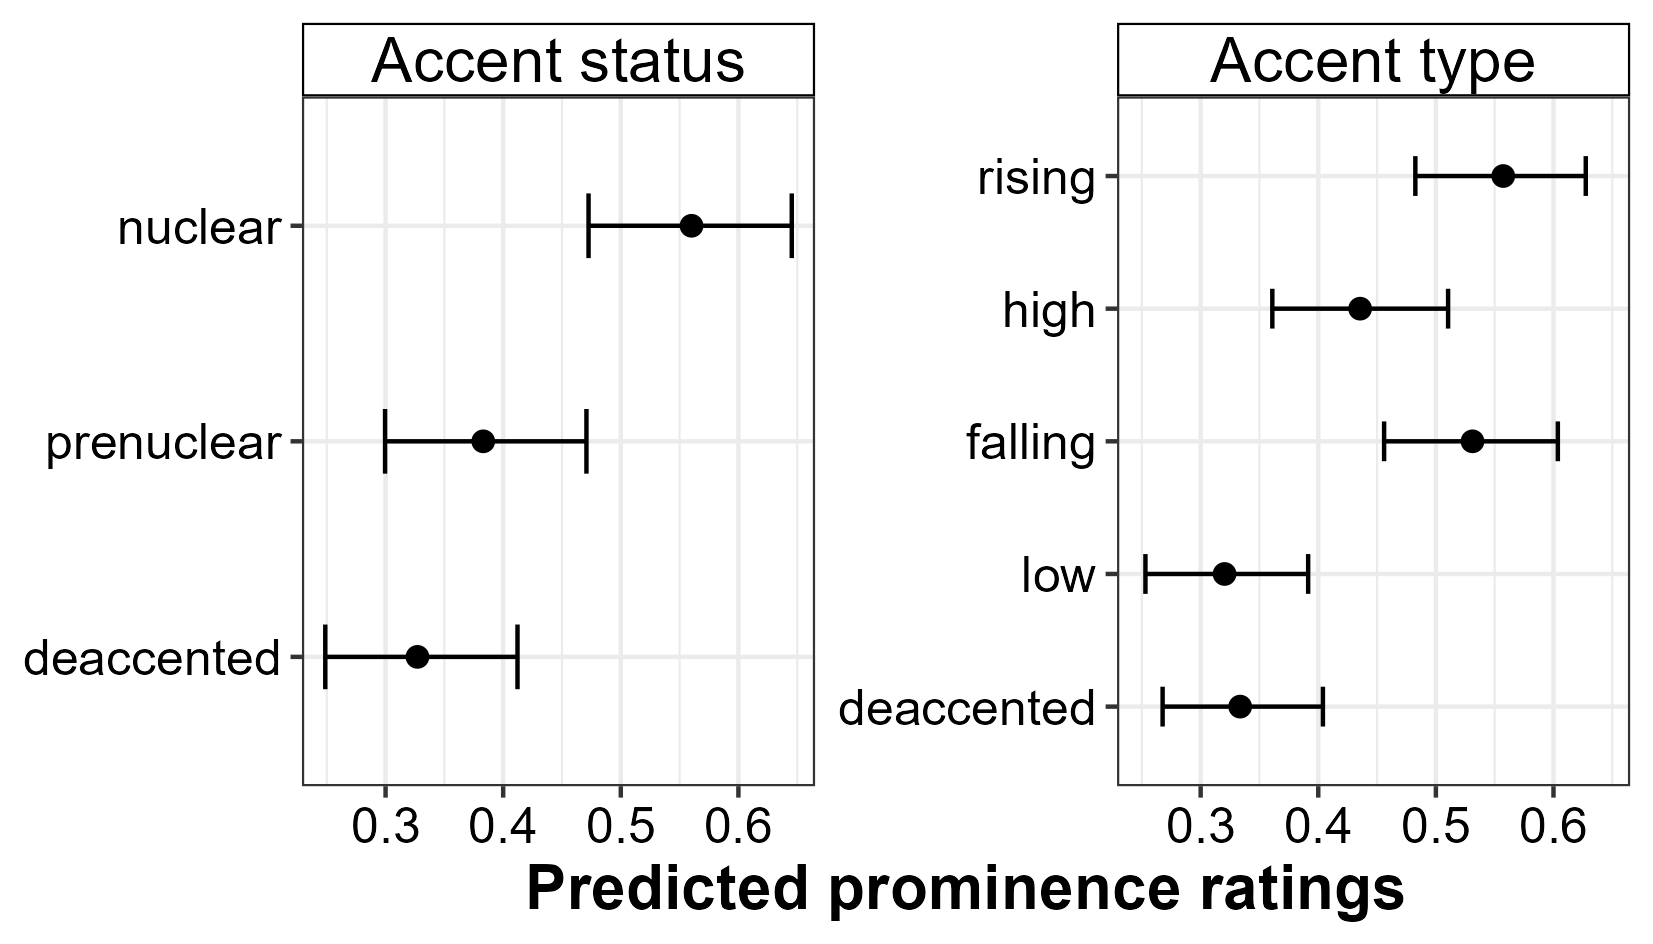
\includegraphics[scale = 0.6]{s3_cat_pros_prmtrs}
	\caption{Mean predicted prominence ratings and 90\% CrIs of the categorical prosodic parameters.}
	\label{fig:s3_cat_pros_prmtrs}
\end{figure}

In terms of accent type, rising accents receive on average the highest prominence ratings, followed by falling and high accents respectively, while low accents and deaccented words are rated least prominent (see Figure \ref{fig:s3_cat_pros_prmtrs}, right). There is a clear advantage for more dynamic accent types, i.e., rising and falling, to be perceived as most prominent, with the direction of pitch movement being of secondary importance. Both rising and falling accents are reliably rated as more prominent than high accents (for rising vs. high: $\beta$ = 0.11, CrI = [0.08; 0.14], Pr($\beta$\textgreater{}0) = 1, for falling vs. high: $\beta$ = 0.09, CrI = [0.06; 0.12], Pr($\beta$\textgreater{}0) = 1). The difference between falling and rising accents is not quite reliable ($\beta$ = 0.02, CrI = [0.0; 0.04], Pr($\beta$\textgreater{}0) = 0.95) but nevertheless provides strong evidence that rising accents are perceived as more prominent than falling ones. Pitch height also plays a role for prominence ratings since high accents are reliably rated as more prominent than low accents ($\beta$ = 0.12, CrI = [0.08; 0.17], Pr($\beta$\textgreater{}0) = 1) or deaccented words ($\beta$ = 0.10, CrI = [0.07; 0.14], Pr($\beta$\textgreater{}0) = 1). Although low accents are on average rated lower in prominence than deaccented words, this difference is not reliable ($\beta$ = -0.01, CrI = [-0.05; 0.03], Pr($\beta$\textgreater{}0) = 0.3).

\begin{figure}[b]
		\includegraphics[scale = 0.6]{S3_cont_prmtrs}
	\caption{Mean posterior estimates and 90\% CrIs of the effects of the continuous prosodic parameters on prominence ratings.}
	\label{fig:S3_cont_prmtrs}
\end{figure}

Additionally, all continuous prosodic variables have a reliable influence on prominence ratings (see Figure \ref{fig:S3_cont_prmtrs} and Appendix \ref{Appendix C} for a plot showing predicted prominence ratings by each continuous prosodic parameter). For most continuous variables, higher values coincide with higher prominence ratings. Longer duration, both of the target word and only the stressed syllable of the target word, reliably predicts higher prominence ratings (for word duration: $\beta$ = 0.17, CrI = [0.15; 0.19], Pr($\beta$\textgreater{}0) = 1, for syllable duration: $\beta$ = 0.15, CrI = [0.13; 0.17], Pr($\beta$\textgreater{}0) = 1). Similarly, words with higher intensity and higher periodic energy mass in the stressed syllable are reliably rated more prominent than words with lower intensity and lower periodic energy mass (for intensity: $\beta$ = 0.08, CrI = [0.06; 0.09], Pr($\beta$\textgreater{}0) = 1, for periodic energy mass: $\beta$ = 0.11, CrI = [0.09; 0.12], Pr($\beta$\textgreater{}0) = 1). As for pitch scaling, both static pitch height measured as F0 at CoM and dynamic pitch change (Delta F0) reliably predict prominence ratings, although the effect of F0 at CoM is much stronger than that of Delta F0 (for F0 at CoM: $\beta$ = 0.12, CrI = [0.11; 0.14], Pr($\beta$\textgreater{}0) = 1, for Delta F0: $\beta$ = 0.01, CrI = [0; 0.02], Pr($\beta$\textgreater{}0) = 0.98). In terms of alignment, words associated with higher synchrony values, which correspond to a more rising F0 within the stressed syllable, are reliably rated more prominent than words with lower synchrony ($\beta$ = 0.03, CrI = [0.02; 0.04], Pr($\beta$\textgreater{}0) = 1). However, unexpectedly, words with an earlier CoG reliably receive higher prominence ratings than words with a later CoG ($\beta$ = -0.06, CrI = [-0.08; -0.05], Pr($\beta$\textgreater{}0) = 0).

\begin{figure}[t]
	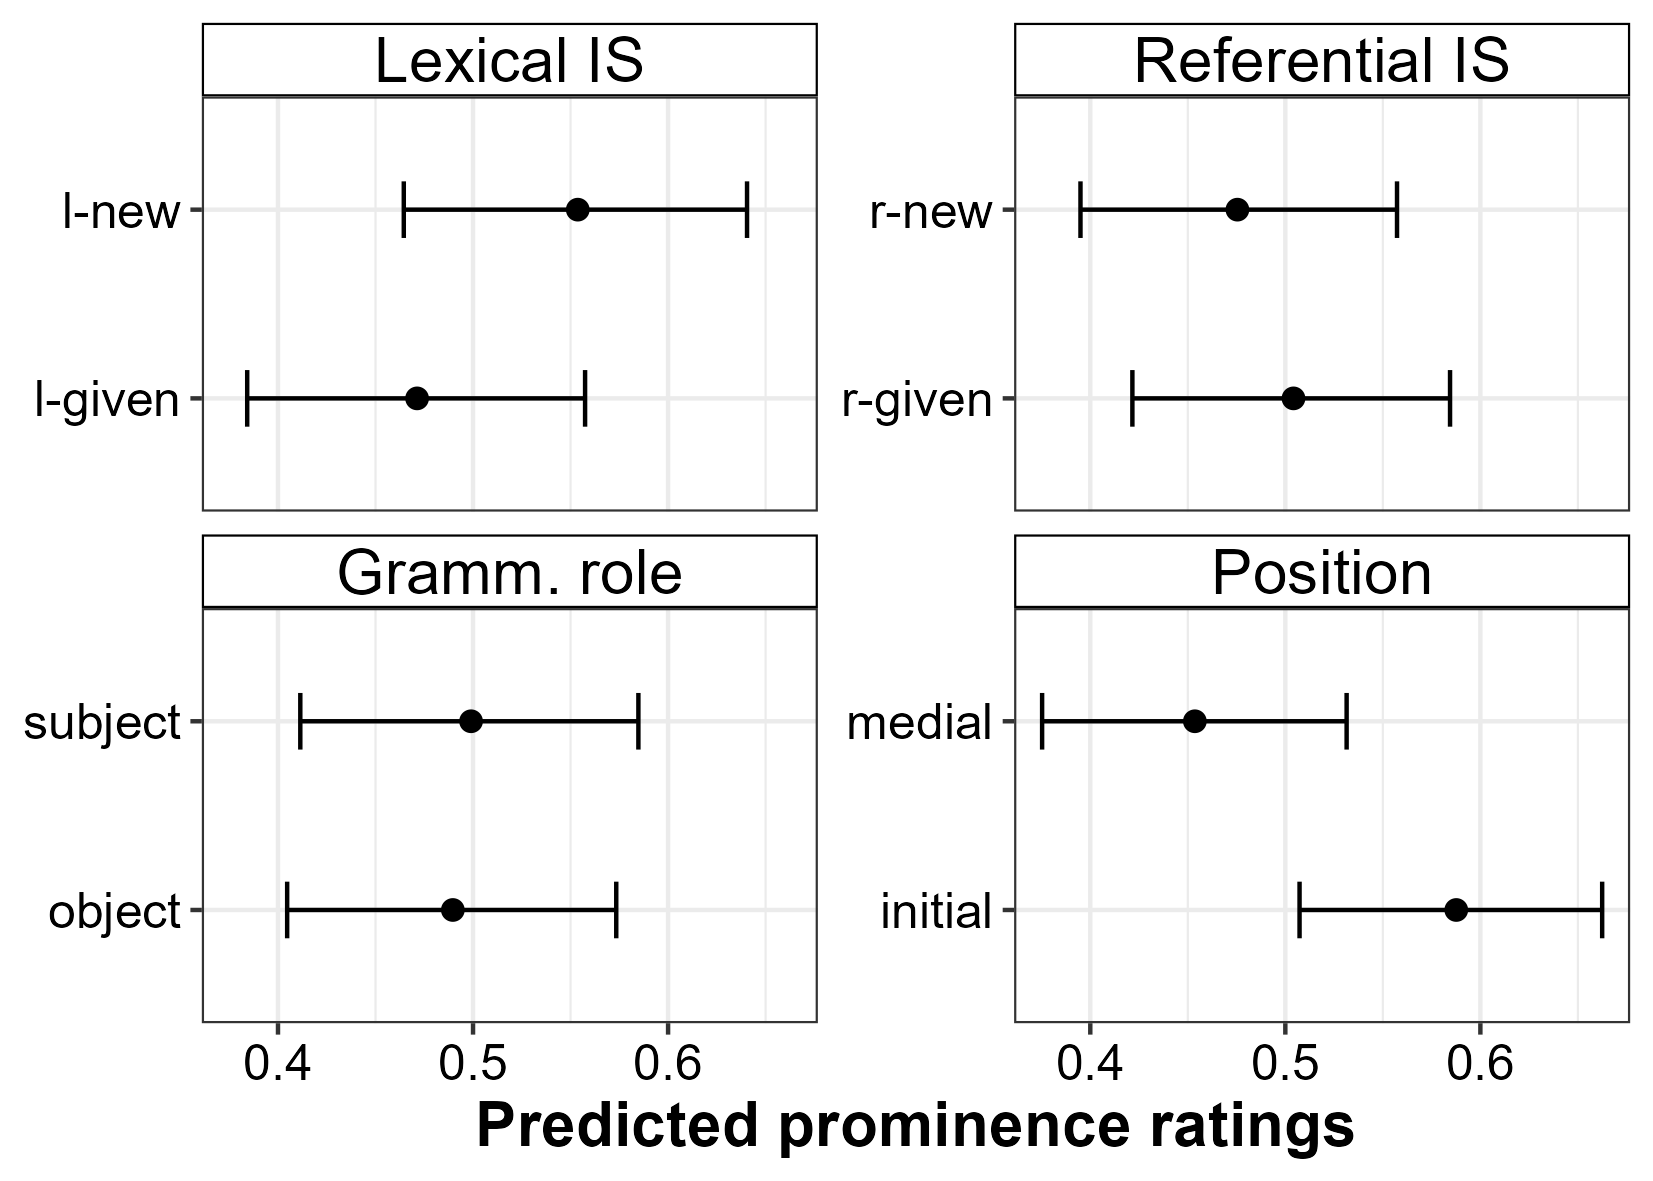
\includegraphics[scale = 0.6]{s3_cat_nonpros_prmtrs}
	\caption{Mean predicted prominence ratings and 90\% CrIs of the non-prosodic parameters.}
	\label{fig:S3_cat_nonpros_prmtrs}
\end{figure}

Finally, we turn to the syntactic and semantic-pragmatic variables. Figure \ref{fig:S3_cat_nonpros_prmtrs} shows the predicted prominence ratings for all four non-prosodic parameters considered here. As expected, lexical newness as opposed to givenness increases prominence ratings across listeners ($\beta$ = 0.08, CrI = [0.06; 0.11], Pr($\beta$\textgreater{}0) = 1). However, the reverse is true for referential information status, with referentially given words reliably rated as more prominent than new ones ($\beta$ = -0.03, CrI = [-0.05; -0.01], Pr($\beta$\textgreater{}0) = 0.01). Grammatical role does not strongly influence prominence ratings ($\beta$ = -0.01, CrI = [-0.03; 0.01], Pr($\beta$\textgreater{}0) = 0.26), but the initial position reliably generates higher prominence ratings than the medial position ($\beta$ = -0.13, CrI = [-0.16; -0.11], Pr($\beta$\textgreater{}0) = 0).

To rank the variables in order of their importance for prominence perception, we turn to random forest analysis \citep[e.g.,][]{breimanRandomForests2001}. The random forest model was first trained on a random subset of 70\% of the data and its predictions were then tested on the remaining 30\% of the data. There is a statistically reliable correlation between the prominence ratings predicted by the random forest model and the actual prominence ratings in the test data ($\beta$ = 0.53, CrI = [0.48; 0.57], Pr($\beta$\textgreater{}0) = 1). The R-squared value we computed (mean R$^2$ = 0.28, CrI = [0.24; 0.31]) indicates that the 14 variables considered in this study account for 28\% of the variance in prominence ratings. 

\begin{figure}
		\includegraphics[scale = 0.7]{S3_random-forest}
	\caption{Variable importance ranking determined by a random forest analysis.}
	\label{fig:S3_random-forest}
\end{figure}

The random forest analysis reveals that accent status is the most important variable in determining prominence ratings across listeners (see Figure \ref{fig:S3_random-forest}). The second discrete prosodic variable, pitch accent type, is also relatively important. Out of the continuous phonetic variables, duration clearly has the largest influence on prominence ratings, especially word duration. CoG and periodic energy mass also rank relatively highly. Delta F0 and intensity are the least important prosodic variables. The syntactic and semantic-pragmatic parameters, by contrast, rank relatively low, the most important of those cues being sentence position, which outranks three of the continuous prosodic cues. Referential information status is slightly more important than lexical information status and grammatical role is the least important variable overall, which is in line with the results of the corresponding regression model.\footnote{Note that the sizes of the parameters' effects on the prominence ratings in the regression models do not necessarily match the results of the random forest analysis. This is due to the fact that some of the parameters are collinear. While the regression models include only one parameter at a time, the random forest analysis takes into account all factors and is thus able to tease apart exactly which parameter contributes most to the prominence ratings and which parameter does not independently contribute. This may explain, for example, why F0 at CoM seems to have a relatively large effect on prominence ratings in the results of the regression models, but ranks below CoG and periodic energy mass in a random forest model that also includes pitch accent type.}

\subsection{Individual strategies}

After reporting on the averaged results across listeners, we turn to the analysis of individual differences (and similarities). Figure \ref{fig:S3_rating_examples} shows exemplary distributions of prominence ratings by four listeners (before scaling). Descriptively, some individuals (e.g., listeners 114 and 150) seem to avoid the middle range of the slider scale, i.e., values around 50, when rating prominence, instead preferring values slightly below or above 50, which leads to bimodal distributions. In the case of listener 114, there seems to be a three-way distinction. This could suggest that prominence is perceived (at least by some individuals) in a more binary or categorical manner, although some gradience in the ratings is also apparent in these listeners. Other listeners (e.g., 151) produce distributions that are closer to normal, which indicates that they treat prominence as more continuous. The inflated use of the end points of the scale (0 and 100), which is typical of scalar rating experiments \citep[e.g.,][]{vuorreHowAnalyzeVisual2019}, is evident in listener 117.

\begin{figure}[b]
	\includegraphics[scale = 0.5]{S3_rating_examples}
	\caption{Prominence ratings by four listeners as examples of differences in the use of visual analogue scales.}
	\label{fig:S3_rating_examples}
\end{figure}

For a systematic approach to individual differences in prominence ratings, we exploit the random by-listener slopes from the regression models presented in the previous section. The random slopes give insight into the extent to which listeners rely on different cues when rating prominence. Running a cluster analysis on the random slopes allows for the identification of potential different listener strategies. The cluster analysis reveals relatively weak evidence for two groups of listeners (average silhouette width: 0.24). Figure \ref{fig:S3_clusters} (left) shows the resulting cluster affiliations in a dendrogram. The majority of listeners (n = 47, 72\% of all listeners) belong to Cluster 1 and Cluster 2 consists of 18 listeners.

\begin{figure}[b]
		\includegraphics[scale = 0.5]{S3_clusters}
	\caption{Results of cluster analysis. Left: Dendrogram showing cluster affiliations of all listeners. Right: Group averages and 90\% CrIs of the posterior estimates for each parameter per cluster.}
	\label{fig:S3_clusters}
\end{figure}

The mean regression coefficients and 90\% CrIs of each variable per cluster are plotted in Figure \ref{fig:S3_clusters} (right). Evidently, the two clusters are very similar in their use of all cues, prosodic and non-prosodic, when rating prominence. Small differences emerge in the extent to which the two clusters rely on certain cues. Listeners in Cluster 2 appear to be more sensitive to accent status and type than those in Cluster 1. Similarly, the prominence ratings of Cluster 2 are also influenced to a stronger degree by synchrony, word and syllable duration, periodic energy mass, and intensity. The remaining continuous prosodic parameters, F0 at CoM, Delta F0, and CoG do not differ much in their effects across clusters, if anything, Cluster 1 relies slightly more on F0 at CoM than Cluster 2. Similar to the trend observed for the prosodic parameters, prominence ratings of Cluster 2 are also more affected by non-prosodic parameters. While the difference across clusters is subtle at best for lexical information status, it is somewhat more pronounced for referential givenness: Both clusters of listeners rate r-given target words more prominent than r-new ones on average, but this effect is stronger for Cluster 2. Similarly, Cluster 2 is more strongly affected by grammatical role and sentence position, although grammatical role does not have a reliable effect on prominence ratings for either cluster and the initial as opposed to the medial position is perceived as more prominent by both clusters.

We trained random forests for each cluster to establish separate variable importance rankings for each group of listeners. These rankings are plotted in Figure \ref{fig:variable_importance_clusters}. The rankings are very similar across clusters, accent status being the most important predictor of prominence ratings in both clusters and intensity and grammatical role the least important ones.  For Cluster 1, word duration is the second most important variable followed by accent type and syllable duration, which corresponds to the ranking observed across all listeners in the overall results. For Cluster 2, accent type is the second most important variable followed by syllable and word duration. The non-prosodic variables rank relatively low for both clusters, sentence position being slightly more important than referential information status for Cluster 2 and the other way around for Cluster 1.

\begin{figure}
		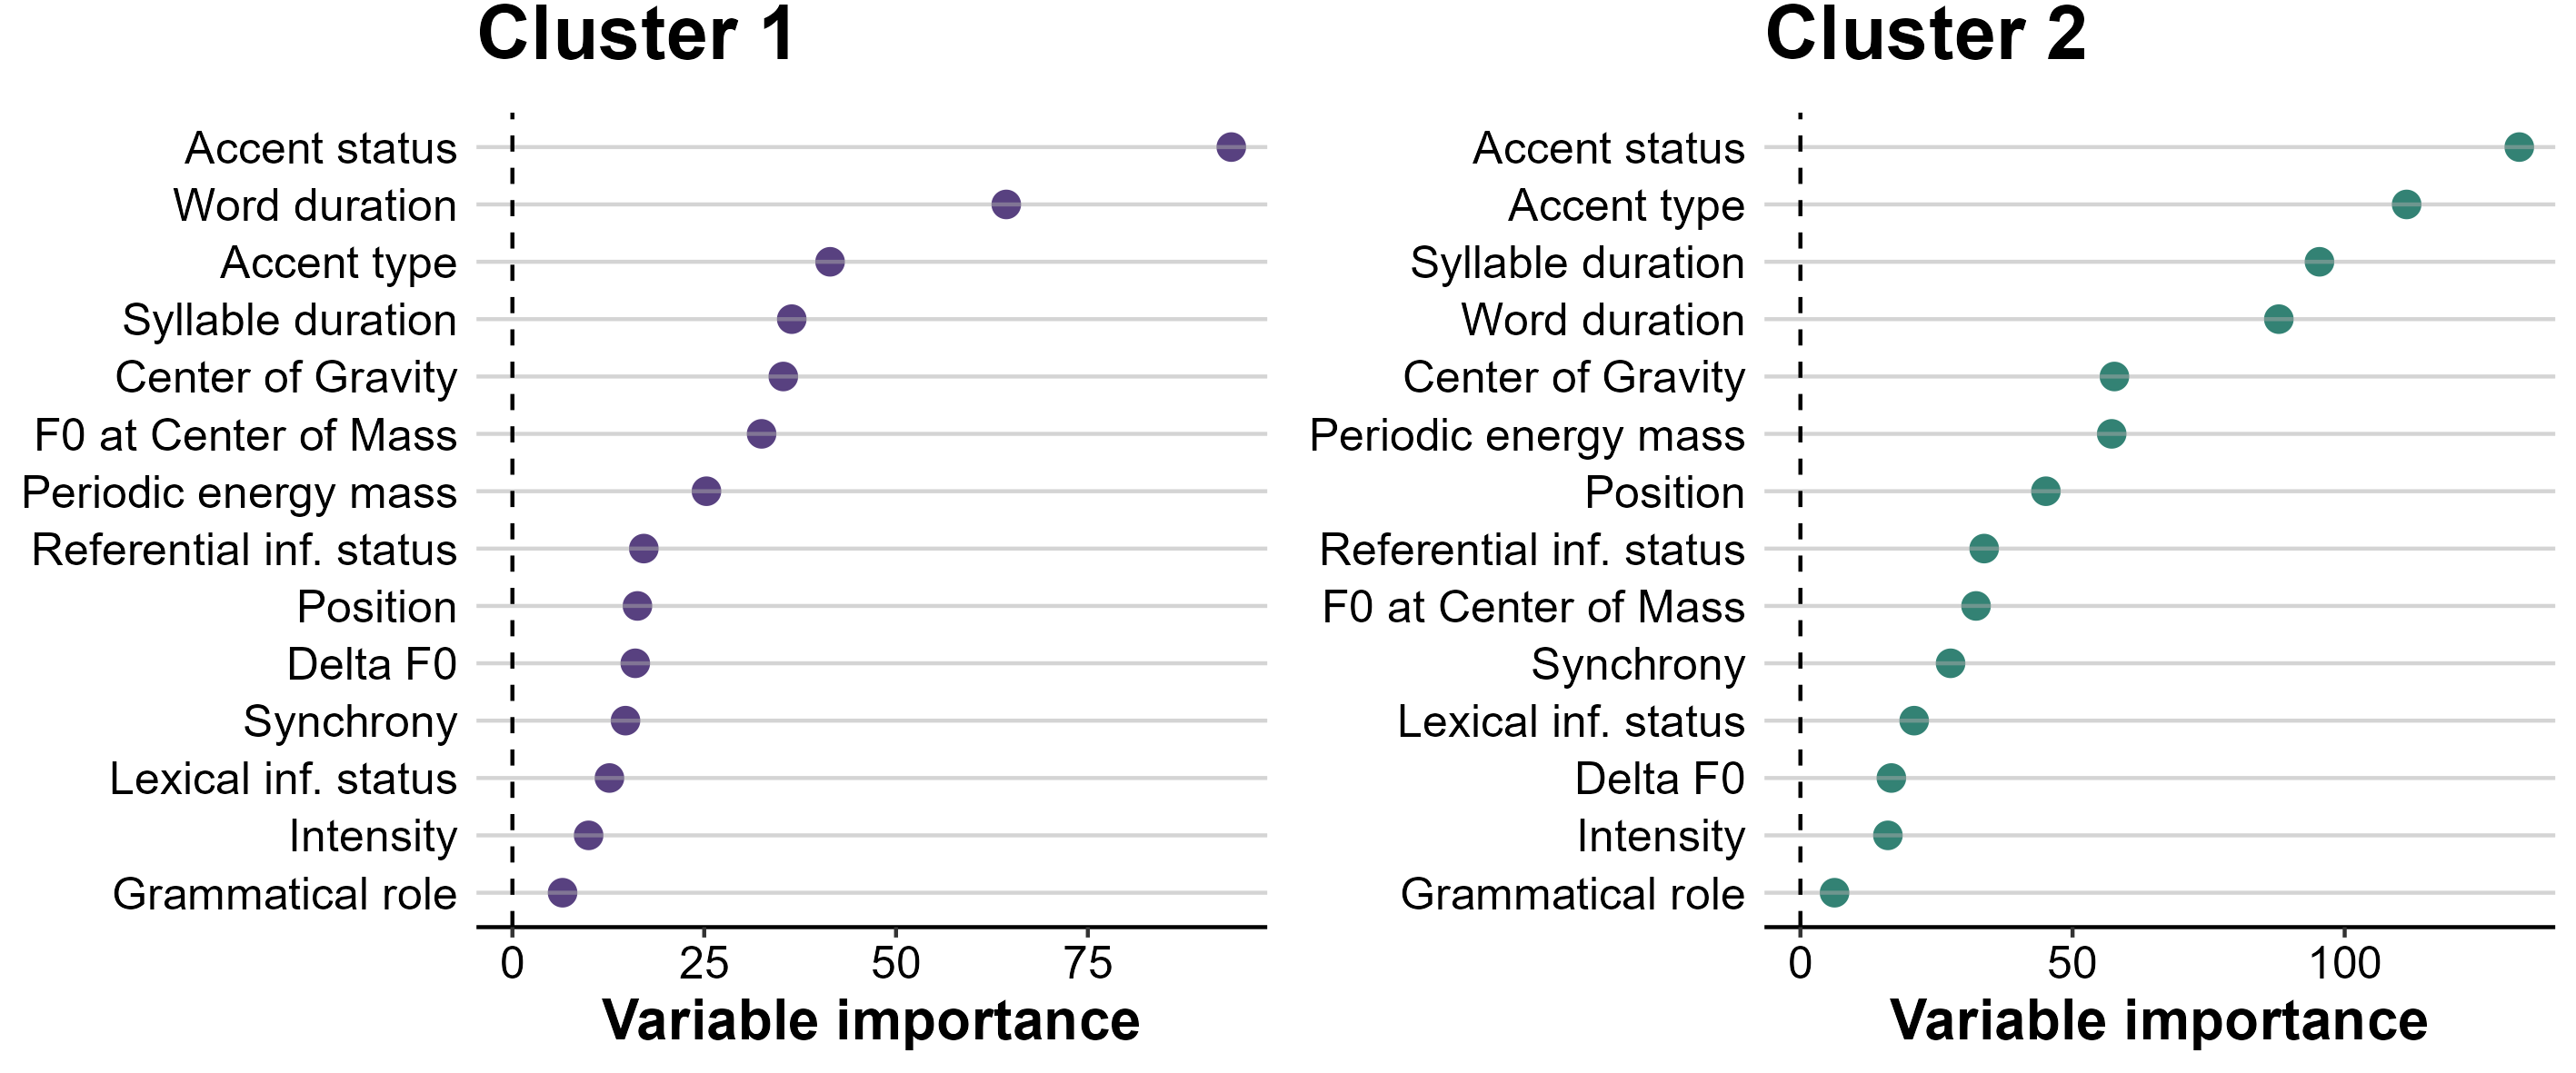
\includegraphics[scale = 0.5]{variable_importance_clusters}
	\caption{Variable importance rankings determined by random forest analyses for each cluster.}
	\label{fig:variable_importance_clusters}
\end{figure}

We again validated the random forest models by testing their predictions on a random subset of 30\% of the data that had been withheld during training. Predicted prominence ratings and actual ratings in the test subset of the data are reliably correlated in both random forests (for Cluster 1: $\beta$ = 0.43, 90\% CrI = [0.37; 0.49], Pr($\beta$\textgreater{}0) = 1, for Cluster 2: $\beta$ = 0.54, 90\% CrI = [0.45; 0.63], Pr($\beta$\textgreater{}0) = 1). We also computed the R-squared values for each cluster as an indication of how much variance is explained by the 14 predictor variables: Cluster 1 is associated with a mean R$^2$ of 0.18 (90\% CrI = [0.14; 0.22]) and Cluster 2 with a mean R$^2$ of 0.29 (90\% CrI = [0.22; 0.36]). The explained variance is thus slightly higher for Cluster 2 than for Cluster 1, in line with the previous observation that this group of listeners is more sensitive to most prominence cues.

As in the second production study presented in Chapter \ref{ch:Production II}, self-assessed communicative scores were collected from all participants. Listeners scored between 1 and 10 points with a mean of 6.4 (SD = 2.0). Generally, listeners with higher communicative scores use higher mean prominence ratings, however, this effect is not reliable for any of the models (e.g., in the accent type model: $\beta$ = 0.01, CrI = [-0.01; 0.02], Pr($\beta$\textgreater{}0) = 0.77). More importantly, we were interested in the interactions between communicative score and the predictor variables, which give insight into the question whether listeners with higher communicative scores are more sensitive to any of the investigated cues in their prominence ratings. Figure \ref{fig:s3_interactions} shows the predicted prominence ratings as a function of the categorical prosodic parameters and communicative score (top) as well as the posterior estimates for the interaction effects of the continuous prosodic cues (bottom left) and the non-prosodic cues (bottom right) with communicative score. 

\begin{figure}
		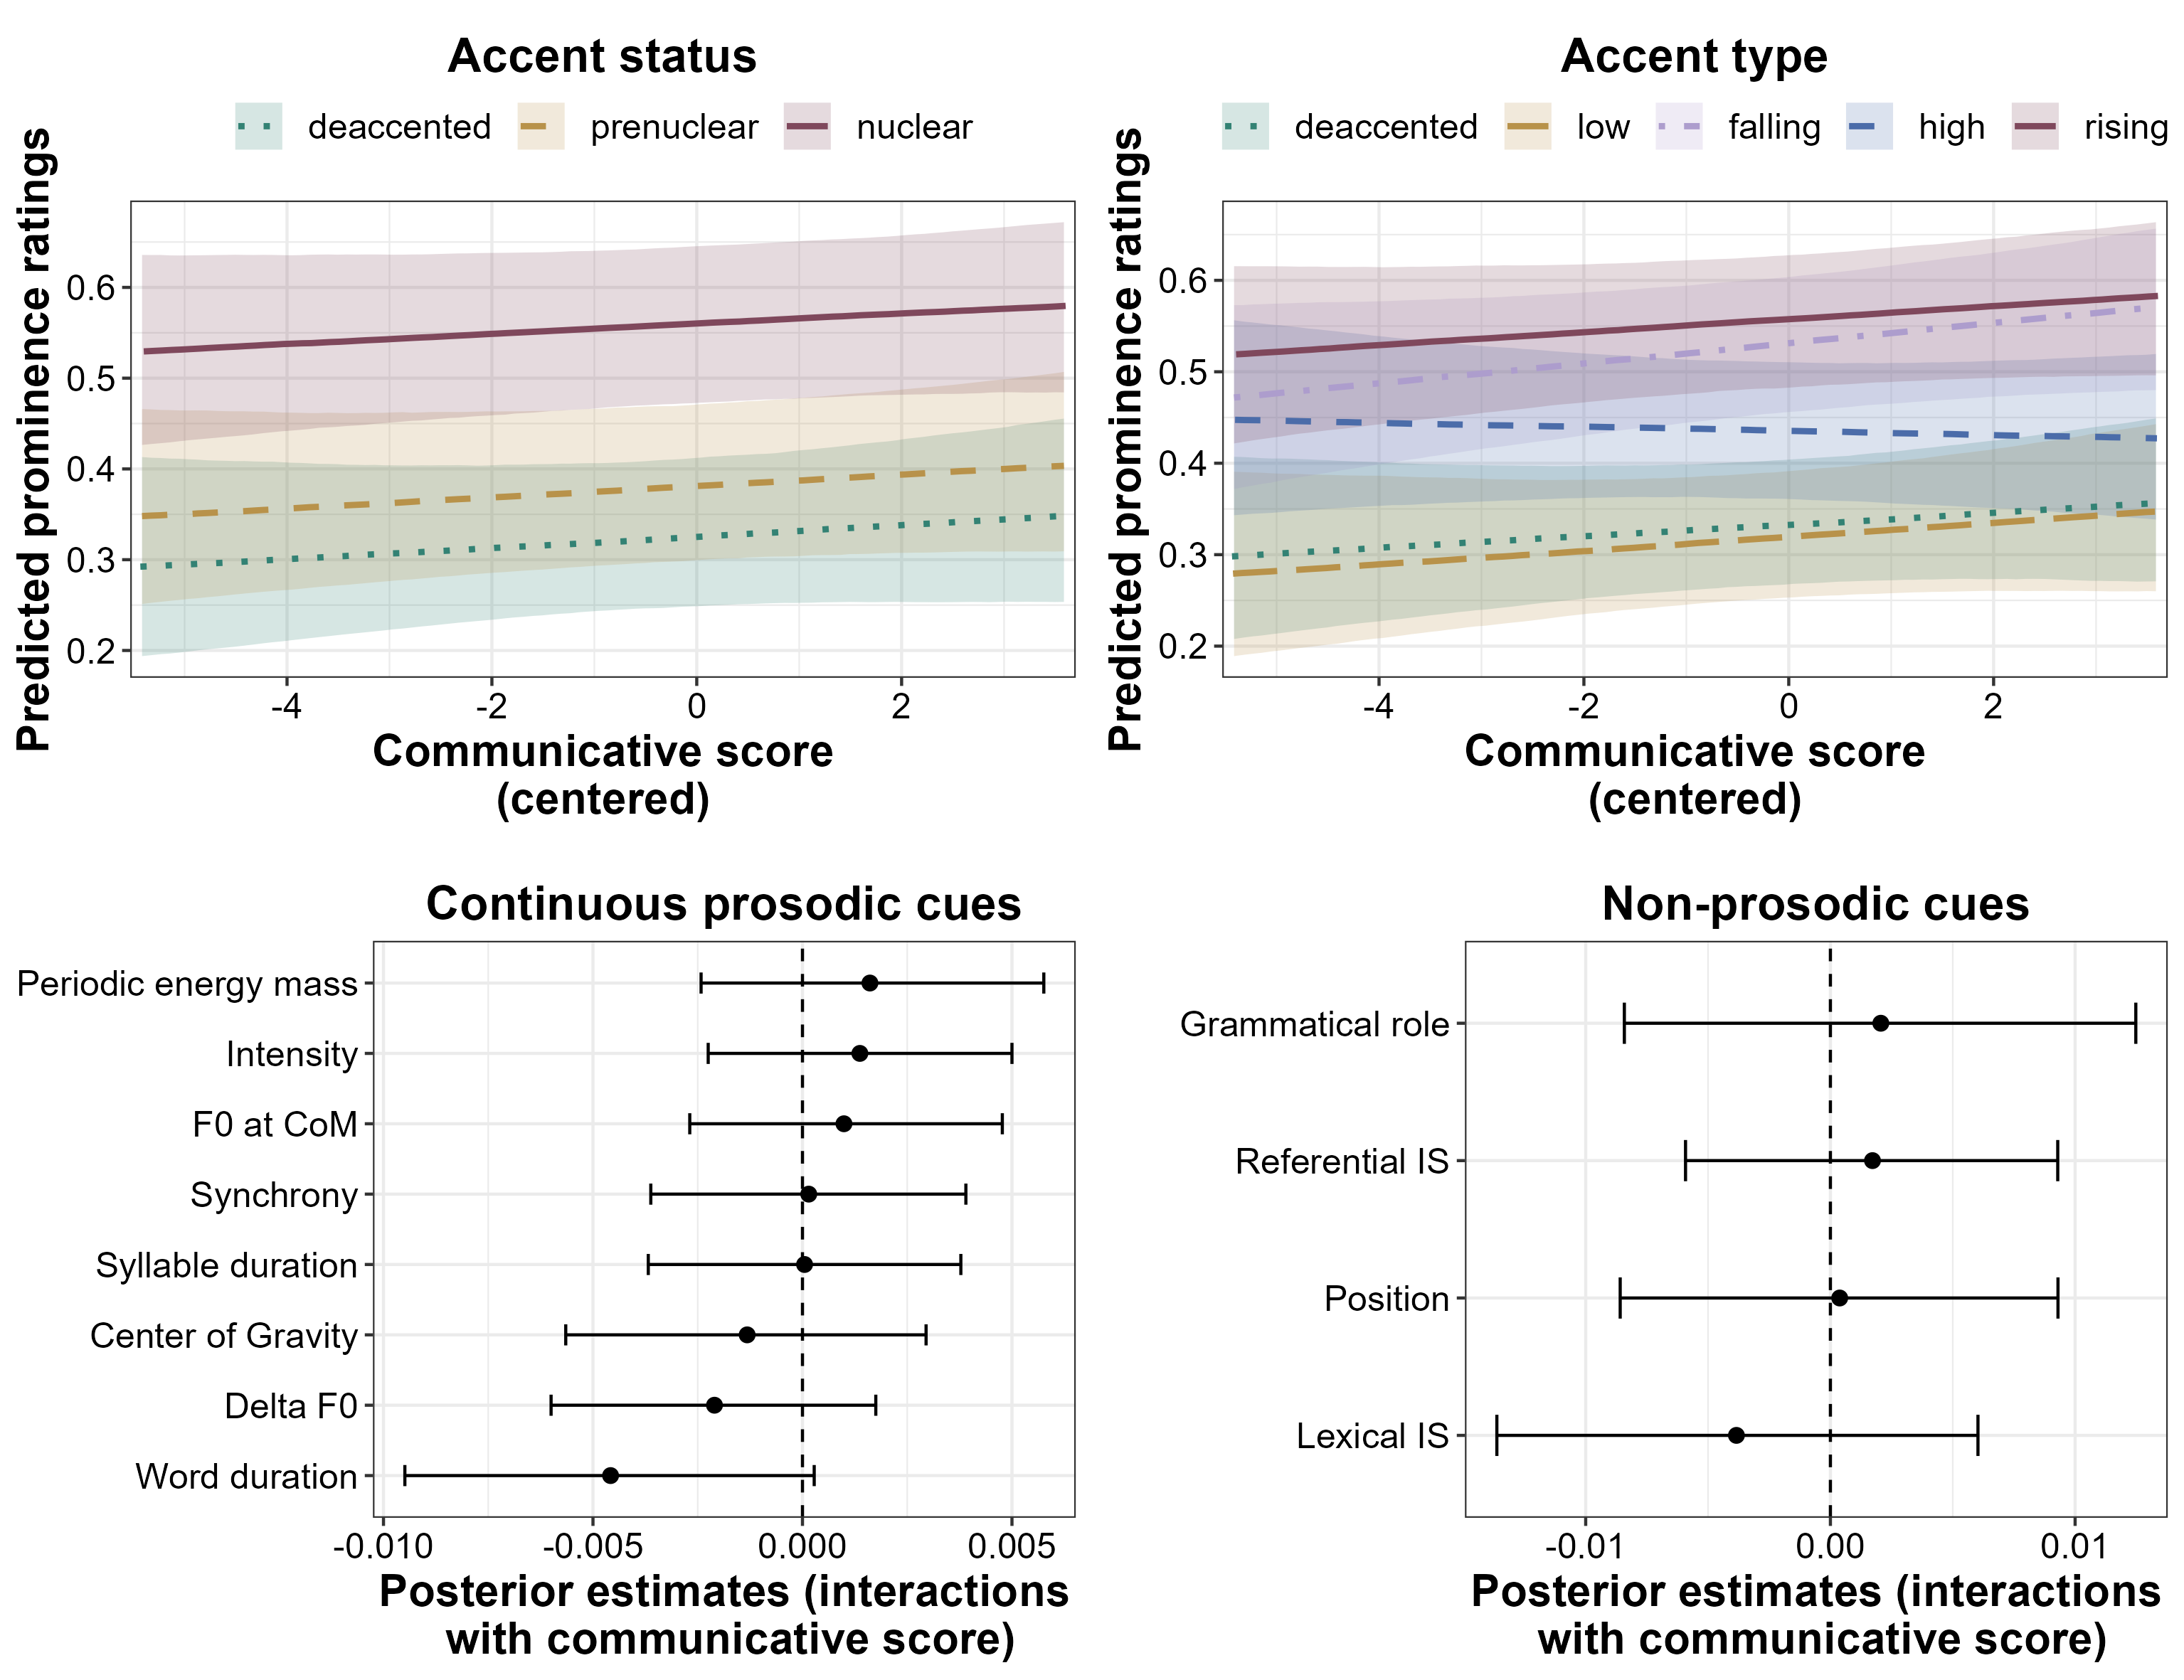
\includegraphics[scale = 0.45]{s3_all_interactions}
	\caption{Interaction effects of the predictor variables and communicative score. Top left: Mean predicted prominence ratings and 90\% CrIs as a function of accent status and communicative score. Top right: Mean predicted prominence ratings and 90\% CrIs as a function of accent type and communicative score. Bottom left: Mean posterior estimates and 90\% CrIs for the interactions of communicative score with the continuous prosodic cues. Bottom right: Mean posterior estimates and 90\% CrIs for the interactions of communicative score with the non-prosodic cues.}
	\label{fig:s3_interactions}
\end{figure}

Since the categorical prosodic cues have multiple levels, we plot the predicted prominence ratings by communicative score for each level (Figure \ref{fig:s3_interactions}, top) and explore them descriptively. The positive main effect of communicative score on prominence ratings is evident from the predominantly positive slopes in the plotted lines. However, for accent status, the three lines for deaccentuation, prenuclear and nuclear accents run in parallel, indicating that there is no interaction between accent status and communicative score. Listeners attend to changes in accent status to the same extent irrespective of their communicative score, only the baseline of prominence ratings is slightly higher for listeners with higher communicative scores. For accent type, we again observe mostly parallel lines with one notable exception: The line associated with the high pitch accent has a slight negative slope, which for listeners with higher communicative scores results in a larger difference in predicted prominence ratings between high and falling/rising accents and a smaller difference between high and low accents/deaccented words. For listeners with lower communicative scores, this effect is reversed: The difference between high and falling/rising accents is smaller for them, while the difference between high and low accents/deaccented words is larger. This may suggest a difference in the perception of accent types with regard to prominence that is modulated by communicative skill. However, note that the credible intervals, which clearly overlap in places, indicate some uncertainty with regard to these observations. Listeners with similar communicative skill are thus not perfectly uniform in their prominence rating behavior. 

In the two bottom plots of Figure \ref{fig:s3_interactions}, posterior estimates indicate how much listeners are influenced by the respective cue in their prominence ratings as a function of communicative score. A mean posterior estimate of 0 indicates that listeners are influenced by a cue to the same extent, irrespective of their communicative score. A positive posterior estimate indicates that listeners with \textit{higher} communicative scores are more strongly influenced by a specific cue in their prominence rating, a negative posterior estimate indicates that listeners with \textit{lower} communicative scores are more strongly influenced by a cue. As is evident from the plots, neither continuous prosodic nor non-prosodic cues reliably interact with communicative score. In fact, many posterior estimates are firmly centered around 0. Out of all these cues, word duration shows the strongest interaction with communicative score, but it is a negative effect: Listeners with lower communicative score are thus more sensitive to differences in word duration when rating prominence. Generally, the results do not provide strong evidence for a consistent effect of communicative score on prominence perception.

Although this is not the primary objective of the present study, a brief note on sociodemographics is in order, since the participants represent a wide range of backgrounds. Table \ref{table:s3_sociodemographics} summarizes the characteristics of listeners in Cluster 1 and 2 in terms of self-reported age, gender, and region of origin.\footnote{The region of origin is based on the federal state in which the participants reported to have grown up in. We classified these states into north and south roughly following the Benrath line.} Listeners in Cluster 1 are younger, more likely female, and from the South than listeners in Cluster 2. However, these differences are relatively small, so that we refrain from drawing any strong conclusions at this point. We will return to this point in the General Discussion in Chapter \ref{ch: general discussion}.

\begin{table}[]
\begin{tabularx}{.9\textwidth}{lYY}
\lsptoprule
                 & Cluster 1 \newline n = 47     & Cluster 2 \newline n = 18     \\ \midrule
Age (median)     & 30                     & 34                     \\
Gender           & 40\% female, 57\% male, 3\% non-binary & 33\% female, 67\% male \\
Region of origin & 28\% north, 72\% south & 39\% north, 61\% south \\
\lspbottomrule
\end{tabularx}
\caption{Sociodemographic characteristics of listeners in the two clusters.}
\label{table:s3_sociodemographics}
\end{table}

\section{Interim discussion} \label{sec:s3_discussion}

In the present study, we confirmed that naive listeners are sensitive to multiple cues in the speech signal when rating prominence on visual analogue scales. Out of 14 potential prosodic and non-prosodic prominence cues, 13 were reliable predictors of prominence. Prosodic cues were especially important in predicting prominence, while syntactic and semantic-pragmatic cues had a much weaker effect on prominence ratings.

The categorical prosodic variables emerged as the strongest cues to perceived prominence, especially accent status but also pitch accent type. This confirms previous findings by \citet{baumannWhatMakesWord2018} and \citet{wagnerExploitingSpeechgestureLink2019} on German as well as \citet{bishopPhonologyPhoneticsSignalextrinsic2020} on American English and provides further independent evidence for the perceptual reality and relevancy of prosodic categories in listeners' processing of prominence. Nuclear accents were clearly perceived as most prominent, while the difference between prenuclear and deaccented words was smaller, underlining the special status of the nuclear accent as a structural cue to prominence \citep[e.g.,][]{buringSemanticsIntonationInformation2007, laddIntonationalPhonology2008}. In terms of pitch accent type, we observed a prevalence of pitch movement over target height: Both rising (L+H*, L*+H) and falling (H+L*, H+!H*) accents were perceived as very prominent, followed by high accents (H*, !H*) and lastly low accents (L*) and deaccented words. This ranking is largely in line with previous observations \citep[e.g.,][]{baumannPerceptualProminencePitch2015, baumannWhatMakesWord2018, bishopPhonologyPhoneticsSignalextrinsic2020}, although some studies have found high accents to be perceived as more prominent than falling accents.

In addition, all continuous variables, capturing aspects of duration, intensity, and fundamental frequency, successfully predicted prominence ratings. Of the continuous parameters, duration was most important, while intensity was the least important predictor of prominence in our study, which is in line with previous studies, such as \citet{fryDurationIntensityPhysical1955, fryExperimentsPerceptionStress1958} and \citet{turkProcessingDurationIntensity1996} but in contrast to \citet{kochanskiLoudnessPredictsProminence2005}. Our study also provides evidence for the validity of the relatively new ProPer measures \citep{albertModelSonorityBased2023} as perceptual correlates of prominence, especially CoG and periodic energy mass. These measures can be derived directly from the signal with no prior annotation, which makes them highly useful for the investigation of larger datasets. With regard to CoG, we expected later alignment to elicit higher ratings, as it has been previously shown that early peaks often correspond to given information, medial peaks to new information and late peaks to unexpected information \citep[e.g.,][]{niebuhrPerzeptionUndKognitive2007}. However, we observed the opposite pattern in that earlier alignment of the CoG elicited higher prominence ratings than later alignment. Interestingly, F0 scaling seemed to add little predictive power independently of pitch accent status and type, which is in line with Fry's (\citeyear[151]{fryExperimentsPerceptionStress1958}) early observation that changes in fundamental frequency ``produce an all-or-none effect" and are interpreted primarily with regard to intonational structure \citep[see also][]{laddProsodicProminenceLanguages2023}.

Of all non-prosodic variables, sentence position was the most important cue to prominence in our listeners, initial target words receiving higher ratings than medial words. Acoustically, the initial position was shown to be produced more prominently than the medial position in Production Study II (see Chapter \ref{ch:Production II}), which partially accounts for the higher ratings. However, the random forest analysis suggests that sentence position also contributed an independent effect. One explanation is that the initial position is less frequent than the medial position in our stimuli and thus more salient through its rarity. In addition, half of the initial stimuli represent a scrambled word order with the grammatical object as initial constituent. In contrast, grammatical role as the second syntactic parameter considered here did not independently contribute to the perception of prominence.

Information status, both lexical and referential, had a relatively small effect on prominence ratings, which could be taken to underline the importance of the prosodic marking of these pragmatic categories. In addition, referential information status behaved opposite to what we expected: Given was perceived as more prominent than new. This could indicate that the short excerpts presented during our task might not have been sufficient for listeners to derive adequate discourse representations or that listeners guided by the task focused more on the prosody of the signal and less on its meaning \citep[e.g.,][]{coleSoundStructureMeaning2019}. Another potential explanation is a mismatch between expectations and prosodic realization: While new referents (at both the lexical and the referential level) would be expected to be produced very prominently by listeners, given referents would be expected to be prosodically attenuated, i.e., deaccented or produced with a prenuclear accent. In the present study, we considered a variety of accent types including nuclear accents on given referents, which are unexpected in this condition. According to \citet{calhounCentralityMetricalStructure2010}, such mismatches in expected and actual prosodic prominence are at the core of prominence perception.

The variables included in the present study as predictors of prominence account for considerably less variability (i.e., 27\%) than previous studies, e.g., by \citet{arnoldUsingGeneralizedAdditive2013}, \citet{baumannWhatMakesWord2018}, and \citet{wagnerExploitingSpeechgestureLink2019}, who accounted for 85\%, 71\%, and 60\% of variability in their respective studies. Some methodological differences to the present study may help explain these discrepancies. For one, \citet{baumannWhatMakesWord2018} and \citet{wagnerExploitingSpeechgestureLink2019} used classic Rapid Prosody Transcription (RPT), where listeners make a binary choice with regard to whether they perceive a word as prominent or not \citep[e.g.,][]{coleSignalbasedExpectationbasedFactors2010}. \citet{arnoldUsingGeneralizedAdditive2013} by contrast obtained prominence ratings on a scale of 0 to 31 from three trained annotators.\footnote{Using prominence scores obtained from trained annotators on visual analogue scales ranging from 0 to 31, \citet{wagnerExploitingSpeechgestureLink2019} were also able to reach 80\% explained variability, similar to \citet{arnoldUsingGeneralizedAdditive2013}.} The use of visual analogue scales, especially by untrained listeners, may introduce more noise than binary RPT ratings. Perhaps more importantly, previous studies included lexical factors, such as part-of-speech and lexical frequency, which were controlled for in our study. Allowing target words to vary in their lexical factors, those studies also included function words, which are generally acoustically not very prominent. As \citet{coleNewMethodsProsodic2016} report, raters are more likely to agree on the absence rather than the presence of prominence, which could have contributed to higher explained variability in those previous studies. In addition, \citet{coleSignalbasedExpectationbasedFactors2010} showed that in American English, lexical frequency is a better predictor of prominence ratings than number of mentions, which is comparable to lexical information status in the present study.

As a further step, we looked at the individual level to reveal potential different strategies in the processing of prominence. However, in contrast to previous studies \citep[e.g.,][]{cangemiListenerSpecificPerceptionSpeakerSpecific2015, bishopIndividualDifferencesTopdown2016, royIndividualDifferencesPatterns2017, baumannWhatMakesWord2018}, we found only subtle individual differences. The main difference between groups of listeners identified via a cluster analysis was the degree of sensitivity to the predictor variables, one group modulating their prominence ratings as a function of these cues a little more than the other group. This was true across prosodic and non-prosodic cues, indicating that the same listeners that were influenced more by prosody also attended more to the syntactic and semantic-pragmatic parameters. This observation is not incompatible with a finding by \citet{orricoInfluenceEmpathyAutisticlike2023}, who report that highly empathetic listeners are more sensitive to the pragmatic distinction of contrastive versus non-contrastive information and highly communicatively skilled individuals are more sensitive to the prosodic contrast of H* versus L+H* accents. Crucially, empathy and communicative skill were correlated in this study, suggesting that the same listeners that were more sensitive to prosody were at the same time more sensitive to pragmatics. Alternatively, higher sensitivity to all types of cues in our study may indicate that some listeners are simply better at performing the prominence rating task, more competent in their use of visual analogue scales or more motivated to perform well.

A plausible explanation for the lack of variability across listeners relates again to the nature of the task: Fairly unambiguously, listeners were asked to rate how highlighted a word sounded, explicitly drawing attention to the acoustic signal. In previous studies \citep[e.g.,][]{baumannWhatMakesWord2018}, the task left more room for interpretation, paraphrasing prominence with terms like ``stressed", ``highlighted" or ``important". That individual differences are minimal in the absence of such alternatives is in line with a finding by \citet{coleSoundStructureMeaning2019} that participants can be guided to focus more on the acoustic signal or the meaning of an utterance by the instructions they receive. Given a straightforward, unambiguous task, which does not lend itself to different interpretations, as is the case in the present study, listeners behave very similarly despite the wide range of cues available to them. In addition, \citet{coleSoundStructureMeaning2019} observed that American English listeners' prominence ratings varied less under different instructions than French or Spanish listeners' ratings. They take this finding to suggest that acoustic prominence and meaning-related factors often coincide in English, which leads to similar prominence ratings under different types of instructions. Assuming a similarly strong link between prosody and meaning in German, this provides further evidence for the concordance of prosodic and non-prosodic cues observed in the present study.

Previous studies \citep[e.g.,][]{bishopPhonologyPhoneticsSignalextrinsic2020, orricoInfluenceEmpathyAutisticlike2023} have noted a correlation between listeners' communicative skill and their ability to perceive prominence distinctions. However, communicative skill did not play an important role in the present study. Nevertheless, some of the tendencies we observed are compatible with the aforementioned previous studies. \citet{bishopIndividualDifferencesTopdown2016} argues that higher communicative skill may specifically be related to a higher sensitivity to pitch but not duration. Our findings support this idea and provide (weak) evidence that listeners with lower communicative skill may in fact be more sensitive to duration. The fact that listeners with lower communicative skill were less sensitive to a distinction between high and rising pitch accents than listeners with higher communicative skill is in line with an observation by \citet{orricoInfluenceEmpathyAutisticlike2023}. \citet{orricoInfluenceEmpathyAutisticlike2023}, who only considered two accent types out of the larger tonal inventory of British English, argue that listeners with lower communicative skill (higher AQ score) mark any accented words as prominent regardless of accent type, which supposedly indicates a poorer integration of context and F0 contour. In the present study, which includes more pitch accent types, we found that listeners with lower communicative skill observed a two-way distinction between rising, high, and falling accents on the one hand and low accents and deaccentuation on the other hand, while listeners with higher communicative skill managed to make a three-way distinction between rising/falling accents, high accents and low accents/deaccentuation.

Most likely, communicative skill (specifically in the way it has been operationalized here) does not fully account for individual variability. A promising avenue for future research is to quantify communicative skill less directly, for example, by measuring performance in tests such as the Reading the Mind in the Eyes test \citep[e.g.,][]{turnbullListenerorientedPhoneticReduction2019}. Another character trait related to communicative skill that may influence the prosody-meaning mapping is empathy \citep[e.g.,][]{esteve-gibertEmpathyInfluencesHow2020, orricoInfluenceEmpathyAutisticlike2023}. \citet{esteve-gibertEmpathyInfluencesHow2020}, for example, found that French listeners with higher empathy scores were more sensitive to intonation as a cue to resolving lexical ambiguities. Additionally, musicality may play a role, especially in pitch perception \citep{schonMusicSpeechMusic2004}. However, future research needs to first and foremost establish the extent of individual variability in prominence perception in the absence of task ambiguities. A comprehensive study should consider prosodic, discourse-related, \textit{and} lexical factors, while controlling for differing task interpretations. Ideally, the task would be communicatively relevant instead of purely metalinguistic to allow participants to form full-fledged discourse representations, which is crucial for the investigation of individual variability in communicative strategies.

\chapter{General discussion} \label{ch: general discussion}

The studies presented in the preceding chapters present exploratory yet systematic analyses of the nature of inter-individual variability in the encoding and decoding of prosodic prominence relations. Two production studies and one perception study investigated individual differences in the mapping of categorical and continuous prosodic cues onto functional aspects of prominence. This chapter discusses the empirical and theoretical contributions of these studies.

\section{Summary of results}

To begin with, this section summarizes the main findings of all three studies. In the first production study presented in Chapter \ref{ch:Production I}, the marking of newness versus accessibility in two subsequent referents was investigated. Results indicated that speakers were rather similar in the type of continuous prosodic parameters used to mark newness, yet differed in their strength of encoding. A cluster analysis revealed a split into two groups, the weak encoders and the strong encoders. In terms of the categorical prosodic parameters, one cluster of speakers was slightly more likely to use accent status as a cue to information status, the other was more likely to use accent type, indicating a weak trade-off effect.

In the second production study presented in Chapter \ref{ch:Production II}, the effects of lexical and referential aspects of information status on prosodic prominence were analyzed separately and the syntactic factors sentence position and grammatical role were additionally included. Individual variability in the encoding of lexical information status was again mostly related to the strength of prosodic marking, while there was more variability in the encoding of the referential level: All speakers used higher periodic energy mass in r-new words, but one group of speakers additionally relied on F0 contour shape and alignment, while the other group used F0 scaling. There were even more diverse strategies in the prosodic marking of grammatical role and sentence position, which mostly related to strength of encoding but also to the type of cue used. In addition, there was a trade-off between the use of accent status and accent type similar to the first study, particularly in the encoding of referential givenness, grammatical role, and sentence position. 

This second production study also considered communicative skill as a potential factor towards explaining individual variability in prosodic form-meaning mapping. As expected, individuals with higher communicative skill produced larger prosodic differences between l-new and l-given referents, especially in terms of accent status, duration, and intensity. However, unexpectedly, the reverse relation was observed for referential information status: Speakers with \textit{lower} communicative skill produced larger differences in terms of accent type and F0 scaling between r-new and r-given words. The results for grammatical role were similar to those for lexical information status, while the prosodic marking of sentence position barely seemed to be influenced by communicative skill.

In the perception study presented in Chapter \ref{ch: Perception}, listeners were asked to rate the perceived prominence in the target words investigated in Production Study II. We found accent status to be the most important cue to prominence followed by duration and accent type, while non-prosodic parameters played only a small role. Individuals did not vary much in their cue rankings, but one group of listeners emerged that was more sensitive to the prominence cues than the other group. However, communicative skill offered little to explain this difference. Only the differentiation of accent types seemed to improve in individuals with higher communicative skill.

\section{Variability in strength of prominence encoding and decoding effects}

A pattern that was repeatedly found throughout all experiments is that a smaller group of speakers or listeners more strongly marks meaning contrasts via prosody or is more sensitive to prominence cues in perception, while a larger group shows the same effects in a more subtle way. This is in line with previous findings, for example, by \citet{roessigDynamicsIntonationCategorical2019}, who observed that a larger group of speakers produced smaller distinctions between focus types in terms of tonal onglide and a smaller group produced larger differences. In general, such findings may help explain why prosodic effects in empirical studies averaged across multiple individuals are often subtle and sometimes inconsistent. Thinking of strength of prosodic encoding as a continuum, where speakers occupy different places between the endpoints ``no encoding" and ``strong encoding", a reasonable relation can be drawn to Lindblom's \citeyearpar{lindblomExplainingPhoneticVariation1990} classic H\&H theory. Specifically, strength of encoding may be related to different weightings of the hyperarticulation and hypoarticulation principles. A higher weighting of the hyperarticulation principle thereby reflects higher listener orientation \citep{turnbullListenerorientedPhoneticReduction2019} and one way this may manifest is in a stronger prosodic marking of meaning-related contrasts. Assuming that communicative skill is a correlate of higher attentiveness towards listener needs, we see a confirmation of this general principle in Production Study II: Higher communicative skill correlates with stronger prosodic differentiation of lexical newness and givenness as well as grammatical object and subject function. 

These considerations would suggest that some speakers are better communicators than others, as has been suggested, for example, by \citet{cangemiListenerSpecificPerceptionSpeakerSpecific2015}. However, data presented in Production Study II indicate that this generalization is too simple. Instead of being generally good or bad communicators, individuals may just differ in how well they encode specific aspects of meaning. This is evident in the clustering results, where strong encoders of lexical information status overlap only marginally with strong encoders of referential givenness. Furthermore, the converse effects of communicative skill on lexical and referential information status marking suggest that different skill sets facilitate the encoding of different meaning contrasts.

Communicative skill could also be interpreted as a superior ability to weigh listener needs (Lindblom's hyperarticulation) against required effort in production (Lindblom's hypoarticulation). Similar to the H\&H theory, the Smooth Signal Redundancy Hypothesis (SSRH) argues that speakers weigh language redundancy against prosodic prominence in order to achieve robust communication \citep{aylettSmoothSignalRedundancy2004}. Interpreted in this light, the weaker prosodic encoding of referential givenness in speakers with higher communicative skill could be explained by their awareness of the presence of another cue, morphosyntactic marking, which encourages prosodic hypoarticulation. That prosodic markers may be weighed against non-prosodic factors is also in line with a finding by \citet{giovannoneIndividualDifferencesLexical2023} that listeners are able to trade off lexical and acoustic information in speech perception.

An alternative explanation relates directly to the communicative situations established in the production studies: Speakers were asked to produce texts in a listener-oriented manner, so that their presumed fellow participants could then fulfil a comprehension task. This set-up could encourage speakers with higher communicative skill to hyperarticulate every content word in order to help the listener memorize the relevant information, similar to a child-directed speech style \citep[e.g.,][]{cristiaInputLanguagePhonetics2013}. We see traces of such behavior in individual speakers that frequently produce phrase boundaries after target words or L+H* accents across conditions, for example, s31 in Production Study I or s08 in Production Study II. The failure to prosodically differentiate r-new from r-given referents would thus result from both words being produced highly prominently. However, our data indicate that r-new referents are rather produced with reduced prominence in such cases, not providing sufficient evidence for this potential explanation. 

In perception, communicative skill has initially been interpreted as an enhanced ability to interpret pragmatic information, i.e., speaker-intended meaning \citep{nieuwlandIncrementalityPragmaticProcessing2010, bishopIndividualDifferencesTopdown2016}. However, recent research has also postulated a relation between communicative skill and sensitivity to prosodic differences \citep{bishopPhonologyPhoneticsSignalextrinsic2020, orricoInfluenceEmpathyAutisticlike2023}. In the perception study presented in Chapter \ref{ch: Perception}, we did not observe any correlation between communicative skill and reliance on pragmatic information in prominence ratings. In fact, pragmatic cues were among the least important predictors of prominence in all listeners. We did however observe slightly different degrees of sensitivity to differences between pitch accent types, which were modulated by communicative skill. More communicatively skilled listeners were able to make more fine-grained distinctions between accent types. 

Since our prominence rating task did not specifically reference meaning distinctions, it is perhaps unsurprising that we neither observed any strong overall effects of non-prosodic factors nor individual differences in pragmatic reliance \citep[cf.][]{coleListeningSoundListening2014, coleSoundStructureMeaning2019}. In addition, the communicative skill score collected via the AQ questionnaire is somewhat broad and it is unclear to what extent it captures pragmatic skill or prosodic sensitivity. There is a remaining need to tease apart these potentially different aspects of individual communicative skill.

Varying strength of effects observed across individuals in all studies can also be related to the degree of engagement with the task or differences in metalinguistic awareness necessary to perform the tasks. Especially the prominence rating task employed in our perception study explicitly taps into metalinguistic awareness and may thus be subject to such effects. \citet{niebuhrF0basedRhythmEffects2009} argues that more musical individuals are particularly skilled in performing these tasks. However, a musical advantage does not necessarily translate into a linguistic processing benefit \citep{niebuhrF0basedRhythmEffects2009}. More indirect, communicatively meaningful tasks may thus yield additional insights into individual variability in the level of encoding and decoding abilities.

\section{Cue trading and prosodic categories}

Compared to the extent of variability observed with regard to strength of encoding, there seems to be relatively little variability across speakers and listeners in the type of cues that they use. Especially in the perception study, listeners were rather uniform with regard to the importance rankings of prominence cues, with accent status clearly being the most important predictor of prominence ratings for all. This uniformity may be somewhat unexpected considering that trade-off or cue weighting effects, which predominantly relate to the variability regarding the use of different types of (continuous) prosodic parameters, have recently become the primary interest of studies specifically investigating inter-individual differences \citep[e.g.,][]{arvanitiVariabilityOverlapCue2024, severijnenYourVOORnaamNot2024}. 

Nevertheless, we observe some cue trading effects in production between F0 scaling and alignment in Production Study II and accent type and accent status in both Production Study I and II. The latter effect is particularly interesting as it relates to the independency of tune and metrical structure, one of the premises of AM theory \citep{laddIntonationalPhonology2008}. Previous observations regarding cue trading effects have mostly been made in relation to continuous prosodic cues \citep{ipSearchSalienceFocus2021, arvanitiVariabilityOverlapCue2024, severijnenYourVOORnaamNot2024}, although prosodic categories are arguably decisive for the interpretation of intonational meaning \citep{laddIntonationalPhonology2008}. The findings in the present production studies thus add new insights on the nature of individual variability and the possibility of cue trading on a categorical level.

Production Study I also revealed that stronger encoding via continuous phonetic cues does not necessarily correlate with a more consistent use of categorical parameters. Specifically, the speakers that showed stronger effects of information status on continuous measures of F0 were less likely to vary accent status as a function of this meaning contrast. Since accent status was confirmed as the most important perceptual cue to prominence in our perception study \citep[also in line with previous studies by][]{baumannWhatMakesWord2018, wagnerExploitingSpeechgestureLink2019}, this finding further stresses the importance of taking into account categorical prosodic parameters. A lack of correspondence between continuous and categorical parameters could be attributed to the pervasiveness of individual differences in the differentiation of prosodic categories. Even a strong categorical contrast like accentuation is subject to variability. For example, \citet{beckmanArticulatoryEvidenceDifferentiating1994} report that for some but not all speakers nuclear accented syllables are longer than unaccented syllables.

In general, all studies confirm the prevalence of prosodic categories for prominence production and especially perception not just on an overall level but also for the individual. Prosodic categories, such as accent status or pitch accent type, may be especially robust to individual variability as they represent bundles of cues. Listeners with diverse preferences for prosodic cues may still be able to interpret and make use of them as they combine several acoustic dimensions. A similar argument has been advanced by \citet{bruggemanUnifyingSpeakerVariability2017} for TCoG as a cue bundle that more reliably correlates with focus type across speakers of Egyptian Arabic than more isolated F0 measures based on turning points.

\section{Relationality, redundancy, and robustness of communication}

Spoken language has been described as a robust and redundant system \citep{winterSpokenLanguageAchieves2014}, in analogy to a theoretical model in biology \citep{kitanoBiologicalRobustness2004}.\footnote{\citet{winterSpokenLanguageAchieves2014} distinguishes between the terms \textit{redundancy} and \textit{degeneracy}. Redundancy refers to repetitions of the same component, while degeneracy refers to different components performing the same function. Here, we forgo this distinction and use the term redundancy throughout, in line with \citet{jasminTailoredPerceptionIndividuals2020}.} Redundancy refers to the concept of multiple components serving the same function, ensuring the robustness of the system in case of the failure of one component \citep{kitanoBiologicalRobustness2004, winterSpokenLanguageAchieves2014}. Robustness in speech can be understood as optimal transmission of linguistic information resulting in successful communication, especially in the face of noise or variation \citep{winterSpokenLanguageAchieves2014}.

Prosodic prominence specifically can be regarded as highly redundant. Prominence can be expressed by single or multiple cues related to the acoustic dimensions F0, duration, and intensity \citep{kochanskiLoudnessPredictsProminence2005, baumannWhatMakesWord2018, roessigTracingPhoneticSpace2022}, ensuring signal redundancy and thus communicative robustness. Furthermore, the relational nature of prominence contributes to this robustness and allows for some variability in the realization of individual prosodic constituents \citep{terkenFundamentalFrequencyPerceived1991, terkenPerceptionProsodicProminence2000, laddIntonationalPhonology2008}. As long as general prominence relations are preserved, prominence is adequately encoded by the speaker and decodable for the listener. We see evidence for this in Production Study II, where lexically and referentially given target words followed by a nuclear accented verb are variably produced with a prenuclear or no accent, so that a weak-strong prominence relation is preserved in both cases.

Perceptually, prominence as a redundant system facilitates robust communication by encompassing multiple cues serving the same function. Listeners have been shown to be able to make use of a variety of cues to decode prominence in many previous studies \citep{turnbullProminencePerceptionDependent2017, baumannWhatMakesWord2018, coleSoundStructureMeaning2019, wagnerExploitingSpeechgestureLink2019}. Our own perception study presented in Chapter \ref{ch: Perception} confirms these findings. This mechanism ensures communicative success despite the general lack of invariance in prosody-meaning mapping \citep{winterSpokenLanguageAchieves2014}. As argued in \citet{baumannWhatMakesWord2018}, listeners need not pay attention to every single cue but can compensate for their inattentiveness to certain parts of the signal by relying on other cues. In listeners who are physically able to perceive and make use of all available acoustic dimensions, such compensatory effects may simply reflect personal preferences for certain cues over others. However, for individuals with perceptual deficits such as congenital amusia, which severely limits pitch perception, functional redundancy crucially enables them to develop successful speech perception strategies by compensating for a missing cue \citep{jasminTailoredPerceptionIndividuals2020}.

Nevertheless, some prominence cues are generally preferred to others. Especially the categorical prosodic variables accent status and accent type are strong cues to prominence. Prosodic categories can be regarded as inherently redundant, since they encompass several acoustic cues (see also previous section). Accent status also conveys the relationality of prominence, as it is the most direct reflection of metrical structure. That is, the strength of the prenuclear or nuclear accent derives from its place in the hierarchical organization of prosodic constituents \citep{laddIntonationalPhonology2008, calhounCentralityMetricalStructure2010}. Naturally, this makes accent status the strongest cue to prominence not only on a general but also at the individual level.

From a production perspective, redundancy enables inter-individual variability. There are many different ways to encode prominence relations and individuals can and do exploit this functional redundancy. The production studies presented in Chapters \ref{ch:Production I} and \ref{ch:Production II} provide evidence that speakers rarely make use of all prosodic parameters available to them to encode a meaning contrast. Instead, they choose different subsets of cues to mark different functional aspects in a compensatory manner. That is, although there is usually some redundancy in the productions of individual speakers, most speakers are not maximally redundant themselves. Redundancy thus at the same time ensures robustness in perception and enables variability in production.

\section{Limitations of the present work and directions for future research}

There are some limitations to the studies presented in this book. Firstly, all production data represent read speech and the perception data is acquired using excerpts of read speech as stimuli. Some differences between read speech and spontaneous speech styles are known. Characteristics of read speech include higher median F0 \citep[English:][]{hazanDoesReadingClearly2010}, steeper declination, and stronger F0 resetting \citep[Swedish:][]{swertsF0DeclinationReadaloud1996}. \citet{baumannCoreferenceLexicalGivenness2013} for German found more early peaks in read speech and more low nuclear accents followed by high boundaries (i.e., continuation rises) in spontaneous speech. Generally, spontaneous and read speech thus appear to differ systematically. However, \citet{grylliaManyShapes2022} observed some variability with regard to the extent that Greek speakers differed between speaking styles: Some speakers produced more animated speech in a reading task, while others did not vary between read versus unscripted speech. Therefore, the distinction between lively and monotonous speech is potentially more relevant for prosody than scriptedness. Lively speech is characterized by more nuclear and more rising accents, steeper F0 excursions. and larger ranges \citep{baumannInformativenessSpeakingStyle2019, chodroffInformationStructureAffect2018}. In our production studies, we elicited such lively speech via listener-directed tasks. Nevertheless, there may be other disadvantages to read speech: \citet{bardDissociationDeaccentingGivenness1999} observed that deaccentuation of second mentions and repetitions rarely occurred within sentences of the same structure in unscripted speech. Spontaneous data could thus offer new insights into the encoding of information status that are not available in scripted speech. 

The presented studies are exclusively concerned with the spoken modality. However, gestures may additionally function as visual cues to prominence \citep{krahmerEffectsVisualBeats2007, ambrazaitisMultimodalProminencesExploring2017, esteve-gibertTimingHeadMovements2017, rohrerVisualizingProsodicStructure2023}. As such, visual cues add a further dimension of redundancy to prominence, which can be exploited by individuals.
Visual prominence cues may potentially be used as a compensatory strategy by individuals not attending to acoustic cues of prominence. Initial evidence from perception showing that individuals rely on visual cues to different extents comes from \citet{bujokAudiovisualPerceptionLexical2024}. Furthermore, it has been shown that individuals vary with regard to how well they integrate auditory and visual cues \citep[e.g.,][]{wilbiksSpeechNonspeechMeasures2022}. However, production studies explicitly  concerned with individual differences in the use of gesture are currently lacking.

Another interesting remaining question is that of a potential link between production and perception. A relation between robust prosodic encoding and an enhanced ability to decode prosodically encoded contrasts in the same individual could help provide a holistic account of individual variability in prosody. Although we can certainly expect intra-individual variability with respect to which contrasts speakers encode most robustly and decode most proficiently, the production-perception link should remain constant and reflect an individuals' general aptitude for both the encoding and the decoding of a certain meaning contrast. Since different participants were included in the production and perception studies, the present book cannot contribute to this line of research. However, evidence for a production-perception link in previous studies is inconclusive so far (see Section \ref{sec:ind_perception}), so that future studies in this direction need to take an exploratory approach.

Throughout all studies, we have noted sociodemographic characteristics associated with speakers and listeners employing different strategies. No clear patterns emerged with regard to age, gender, and regional effects on prominence production and perception. We observed no systematic age effects, which can possibly be attributed to relatively constrained age ranges in our participants, particularly in the production studies. With regard to gender, the strong encoders of lexical givenness in Production Study II were predominantly female. However, this pattern was not confirmed in the encoding of the other contrasts in the same study nor in the other two studies. Similarly, regional distributions did not systematically map onto differences in prominence encoding and decoding. Therefore, we assume that any individual variability observed in the present data is independent of the sociodemographic characteristics of participants and truly idiosyncratic. However, studies with more controlled, properly stratified participant samples could yield further insights into this issue. 

In general, the observations reported in the present book need to be extended beyond laboratory studies to more natural speech in production and communicatively relevant tasks in perception. More natural speech almost necessarily entails speech in face-to-face interaction accompanied by the visual modality, which offers a further avenue of investigation into the redundant nature of prominence. In addition, more differentiated measures of personality traits and abilities could offer new insights into underlying reasons for individual variability, which is likely to also emerge in such settings.

\section{Conclusion} \label{sec: conclusions}

The present book contributes to the study of inter-individual differences in prominence production and perception, which has recently seen considerable interest in the speech prosody community \textendash{} and for good reasons. Individual variability emerged in all three studies presented here, although speakers and listeners were not necessarily drastically different from a group-level average. This is reassuring for many studies not explicitly considering the individual. Nevertheless, acknowledging and describing individual differences is necessary to achieve empirical accuracy since prosodic form-meaning mapping rarely looks the same for or is interpreted in exactly the same way by every single individual. This caveat is especially relevant in light of the drive for ever larger data sets, perpetuating the risk of losing sight of the individual. Understanding individual variability also allows us to refine theoretical assumptions and provides new perspectives on already established concepts in prosodic theory, such as the dichotomy of tune and metrical structure, relationality and redundancy in prominence encoding and decoding, and probabilistic form-meaning mapping. The present work has shown potential avenues into this large endeavor. 
\appendix

\chapter{Supplement to Production Study I} 
\label{Appendix A}

\section{Reading material}

\textbf{Story 1}: Lehrer `teacher' – Geige `violin'\\

NEW-NEW:

\begin{enumerate}
\item Peter ist richtig müde von der Arbeit.
\item Er hat den ganzen Tag im Fundbüro für Besucher Gegenstände herausgesucht.
\item Unter anderem hat er einem Lehrer eine Geige gezeigt.
\item Jetzt ruht er sich vor dem Fernseher aus.
\end{enumerate}

NEW-ACCESSIBLE:

\begin{enumerate}
\item Peter ist richtig müde von der Arbeit.
\item Er hat heute dutzende Besucher durch die kleine Instrumentensammlung im Stadtmuseum geführt.
\item Unter anderem hat er einem Lehrer die Geige gezeigt.
\item Jetzt ruht er sich vor dem Fernseher aus.
\end{enumerate}

ACCESSIBLE-NEW:

\begin{enumerate}
\item Peter ist richtig müde von der Arbeit.
\item Er hat heute eine Schulklasse durch das historische Stadtmuseum geführt.
\item Unter anderem hat er dem Lehrer eine Geige gezeigt.
\item Jetzt ruht er sich vor dem Fernseher aus.
\end{enumerate}

ACCESSIBLE-ACCESSIBLE:

\begin{enumerate}
\item Peter ist richtig müde von der Arbeit.
\item Er hat heute eine Schulklasse durch die kleine Instrumentensammlung im Stadtmuseum geführt.
\item Unter anderem hat er dem Lehrer die Geige gezeigt.
\item Jetzt ruht er sich vor dem Fernseher aus.
\end{enumerate}

\textbf{Story 2}: Nonne `nun' – Mühle `mill'\\

NEW-NEW:

\begin{enumerate}
\item Tom ist richtig müde von der Arbeit.
\item Er hat den ganzen Tag Touristen durch das Stadtmuseum geführt.
\item Unter anderem hat er einer Nonne eine Mühle gezeigt.
\item Jetzt setzt er sich zum Entspannen in seinen Lieblingssessel.
\end{enumerate}

NEW-ACCESSIBLE:

\begin{enumerate}
\item Tom ist richtig müde von der Arbeit.
\item Er hat heute dutzende Besucher durch das Brotmuseum geführt.
\item Unter anderem hat er einer Nonne die Mühle gezeigt.
\item Jetzt setzt er sich zum Entspannen in seinen Lieblingssessel.
\end{enumerate}

ACCESSIBLE-NEW:

\begin{enumerate}
\item Tom ist richtig müde von der Arbeit.
\item Er hat heute eine Gruppe aus der Klosterschule durch das Stadtmuseum geführt.
\item Unter anderem hat er der Nonne eine Mühle gezeigt.
\item Jetzt setzt er sich zum Entspannen in seinen Lieblingssessel.
\end{enumerate}

ACCESSIBLE-ACCESSIBLE:

\begin{enumerate}
\item Tom ist richtig müde von der Arbeit.
\item Er hat heute eine Gruppe aus der Klosterschule durch das Brotmuseum geführt.
\item Unter anderem hat er der Nonne die Mühle gezeigt.
\item Jetzt setzt er sich zum Entspannen in seinen Lieblingssessel.
\end{enumerate}

\textbf{Story 3}: Anwalt `lawyer' – Säge `saw'\\

NEW-NEW:

\begin{enumerate}
\item Jana ist richtig müde von der Arbeit.
\item Sie hat den ganzen Tag im Fundbüro für Kunden Gegenstände herausgesucht.
\item Unter anderem hat sie einem Anwalt eine Säge gezeigt.
\item Jetzt setzt sie sich mit einem Buch auf ihr Sofa.
\end{enumerate}

NEW-ACCESSIBLE:

\begin{enumerate}
\item Jana ist richtig müde von der Arbeit.
\item Sie hat heute dutzende Besucher durch die kleine historische Werkzeugsammlung im Museum geführt.
\item Unter anderem hat sie einem Anwalt die Säge gezeigt.
\item Jetzt setzt sie sich mit einem Buch auf ihr Sofa.
\end{enumerate}

ACCESSIBLE-NEW:

\begin{enumerate}
\item Jana ist richtig müde von der Arbeit.
\item Sie war heute bei einem Gerichtsprozess für die Beweisstücke zuständig.
\item Unter anderem hat sie dem Anwalt eine Säge gezeigt.
\item Jetzt setzt sie sich mit einem Buch auf ihr Sofa.
\end{enumerate}

ACCESSIBLE-ACCESSIBLE:

\begin{enumerate}
\item Jana ist richtig müde von der Arbeit.
\item Sie war heute bei einem Gerichtsprozess für die Beweisstücke zum Mord im Baumarkt zuständig.
\item Unter anderem hat sie dem Anwalt die Säge gezeigt.
\item Jetzt setzt sie sich mit einem Buch auf ihr Sofa.
\end{enumerate}
 
\textbf{Story 4}: Bauer `farmer' – Birne `pear'\\

NEW-NEW:

\begin{enumerate}
\item Nach zwei regnerischen Wochen schien endlich wieder die Sonne.
\item Maria hat sich ihre Schuhe angezogen und ist spazieren gegangen. 
\item Unterwegs hat sie einem Bauern eine Birne geschenkt.
\item Jetzt ist sie wieder zu Hause und kocht sich einen Tee.
\end{enumerate}

NEW-ACCESSIBLE:

\begin{enumerate}
\item Nach zwei regnerischen Wochen schien endlich wieder die Sonne.
\item Nachdem Maria ein paar Früchte eingesteckt hatte, ist sie spazieren gegangen.
\item Unterwegs hat sie einem Bauern die Birne geschenkt.
\item Jetzt ist sie wieder zu Hause und kocht sich einen Tee.
\end{enumerate}

ACCESSIBLE-NEW:

\begin{enumerate}
\item Nach zwei regnerischen Wochen schien endlich wieder die Sonne.
\item Maria hat sich ihre Schuhe angezogen und ist zwischen den Feldern des benachbarten Gutshofs spazieren gegangen. 
\item Unterwegs hat sie dem Bauern eine Birne geschenkt.
\item Jetzt ist sie wieder zu Hause und kocht sich einen Tee.
\end{enumerate}

ACCESSIBLE-ACCESSIBLE

\begin{enumerate}
\item Nach zwei regnerischen Wochen schien endlich wieder die Sonne.
\item Nachdem Maria ein paar Früchte eingesteckt hatte, ist sie zwischen den Feldern des benachbarten Gutshofs spazieren gegangen.
\item Unterwegs hat sie dem Bauern die Birne geschenkt.
\item Jetzt ist sie wieder zu Hause und kocht sich einen Tee.
\end{enumerate}

\textbf{Story 5}: Maler `painter' – Waage `scale'\\

NEW-NEW:

\begin{enumerate}
\item Anna hatte einen erfolgreichen Tag.
\item Sie hat die Kunden auf dem Flohmarkt für viele ihrer Waren begeistern können.
\item Unter anderem hat sie einem Maler eine Waage verkauft.
\item Jetzt ist sie zu Hause und entspannt sich bei schöner Musik.
\end{enumerate}

NEW-ACCESSIBLE:

\begin{enumerate}
\item Anna hatte einen erfolgreichen Tag im Geschäft.
\item Sie hat die Kunden für die Restbestände bei den Küchengeräten begeistern können. 
\item Unter anderem hat sie einem Maler die Waage verkauft.
\item Jetzt ist sie zu Hause und entspannt sich bei schöner Musik.
\end{enumerate}

ACCESSIBLE-NEW:

\begin{enumerate}
\item Anna hatte einen erfolgreichen Tag.
\item Am Mittag sind einige Handwerker von der Baustelle nebenan in ihr Geschäft gekommen.
\item Unter anderem hat sie dem Maler eine Waage verkauft.
\item Jetzt ist sie zu Hause und entspannt sich bei schöner Musik.
\end{enumerate}

ACCESSIBLE-ACCESSIBLE:

\begin{enumerate}
\item Anna hatte einen erfolgreichen Tag.
\item Am Mittag sind einige Handwerker von der Baustelle nebenan in ihr Geschäft gekommen, um sich die Restbestände bei den Küchengeräten anzusehen.
\item Unter anderem hat sie dem Maler die Waage verkauft.
\item Jetzt ist sie zu Hause und entspannt sich bei schöner Musik.
\end{enumerate}

\textbf{Story 6}: Kellner `server' – Vase `vase'\\

NEW-NEW:

\begin{enumerate}
\item Claudia hatte einen erfolgreichen Tag.
\item Sie hat die Kunden auf dem Flohmarkt für viele ihrer Waren begeistern können.
\item Unter anderem hat sie einem Kellner eine Vase verkauft.
\item Jetzt geht sie nach Hause und legt sich sofort hin.
\end{enumerate}

NEW-ACCESSIBLE:

\begin{enumerate}
\item Claudia hatte einen erfolgreichen Tag.
\item Sie hat die Kunden in ihrem Blumenladen für die restlichen Keramikartikel begeistern können. 
\item Unter anderem hat sie einem Kellner die Vase verkauft.
\item Jetzt geht sie nach Hause und legt sich sofort hin.
\end{enumerate}

ACCESSIBLE-NEW:

\begin{enumerate}
\item Claudia hatte einen erfolgreichen Tag im Geschäft.
\item Sie hat einige Kollegen vom Restaurant nebenan für viele ihrer Waren begeistern können.
\item Unter anderem hat sie dem Kellner eine Vase verkauft.
\item Jetzt geht sie nach Hause und legt sich sofort hin.
\end{enumerate}

ACCESSIBLE-ACCESSIBLE:

\begin{enumerate}
\item Claudia hatte einen erfolgreichen Tag.
\item Sie hat einige Kollegen vom Restaurant nebenan für die restlichen Keramikartikel in ihrem Blumenladen begeistern können.
\item Unter anderem hat sie dem Kellner die Vase verkauft.
\item Jetzt geht sie nach Hause und legt sich sofort hin.
\end{enumerate}
 
\textbf{Story 7}: Oma `grandma' – Mantel `coat'\\

NEW-NEW:

\begin{enumerate}
\item Rudi hatte einen erfolgreichen Tag.
\item An seinem Stand auf dem Flohmarkt sind viele Leute vorbeigekommen.
\item Unter anderem hat er einer Oma einen Mantel verkauft.
\item Jetzt entspannt er sich in der Badewanne.
\end{enumerate}

NEW-ACCESSIBLE:

\begin{enumerate}
\item Rudi hatte einen erfolgreichen Tag.
\item Viele Kunden haben sich in seiner Boutique für die Einzelstücke der Herbst-Kollektion interessiert.
\item Unter anderem hat er einer Oma den Mantel verkauft.
\item Jetzt entspannt er sich in der Badewanne.
\end{enumerate}

ACCESSIBLE-NEW:

\begin{enumerate}
\item Rudi hatte einen erfolgreichen Tag.
\item Unter den Kunden an seinem Stand auf dem Flohmarkt war auch eine Großfamilie.
\item Unter anderem hat er der Oma einen Mantel verkauft.
\item Jetzt entspannt er sich in der Badewanne.
\end{enumerate}

ACCESSIBLE-ACCESSIBLE:

\begin{enumerate}
\item Rudi hatte einen erfolgreichen Tag.
\item Unter den Kunden in seiner Boutique war auch eine Großfamilie, die sich für die Einzelstücke der Herbst-Kollektion interessiert hat.
\item Unter anderem hat er der Oma den Mantel verkauft.
\item Jetzt entspannt er sich in der Badewanne.
\end{enumerate}

\textbf{Story 8}: Sänger `singer' – Kanne `can'\\

NEW-NEW:

\begin{enumerate}
\item Sandra hatte einen erfolgreichen Tag.
\item An ihrem Stand auf dem Flohmarkt sind viele Leute vorbeigekommen.
\item Unter anderem hat sie einem Sänger eine Kanne verkauft.
\item Jetzt kocht sie sich Nudeln zum Abendessen.
\end{enumerate}

NEW-ACCESSIBLE:

\begin{enumerate}
\item Sandra hatte einen erfolgreichen Tag in ihrem Teeladen.
\item Einige Kunden haben sich für die Einzelstücke der Porzellankollektion aus dem Vorjahr interessiert.
\item Unter anderem hat sie einem Sänger die Kanne verkauft.
\item Jetzt kocht sie sich Nudeln zum Abendessen.
\end{enumerate}

ACCESSIBLE-NEW:

\begin{enumerate}
\item Sandra hatte einen erfolgreichen Tag auf dem Flohmarkt.
\item Es war viel los und wie immer gab es auch ein Live-Konzert. 
\item Unter anderem hat sie dem Sänger eine Kanne verkauft.
\item Jetzt kocht sie sich Nudeln zum Abendessen.
\end{enumerate}

ACCESSIBLE-ACCESSIBLE:

\begin{enumerate}
\item Sandra hatte einen erfolgreichen Tag auf dem Flohmarkt. 
\item Wie immer gab es auch ein Live-Konzert und einige Leute haben sich für das alte Teeservice ihrer Oma interessiert.
\item Unter anderem hat sie dem Sänger die Kanne verkauft.
\item Jetzt kocht sie sich Nudeln zum Abendessen.
\end{enumerate}

\textbf{Practice stories}\\

Rabbi `rabbi' - Angel `fishing rod'\\

NEW-NEW:

\begin{enumerate}
\item Georg ist müde von der Arbeit.
\item Er hat den ganzen Tag im Fundbüro für Besucher Gegenstände herausgesucht.
\item Zum Schluss hat er einem Rabbi eine Angel gezeigt.
\item Jetzt geht er in seine Lieblingskneipe.
\end{enumerate}

Mutter `mother' - Lampe `lamp'\\

NEW-NEW:

\begin{enumerate}
\item Heute Morgen waren viele Kunden im Geschäft.
\item David war die ganze Zeit damit beschäftigt, Fragen zu beantworten.
\item Dann hat er einer Mutter eine Lampe verkauft.
\item Jetzt macht er Mittagspause.
\end{enumerate}

\newpage

\section{Accent types by speaker}

\begin{figure}
		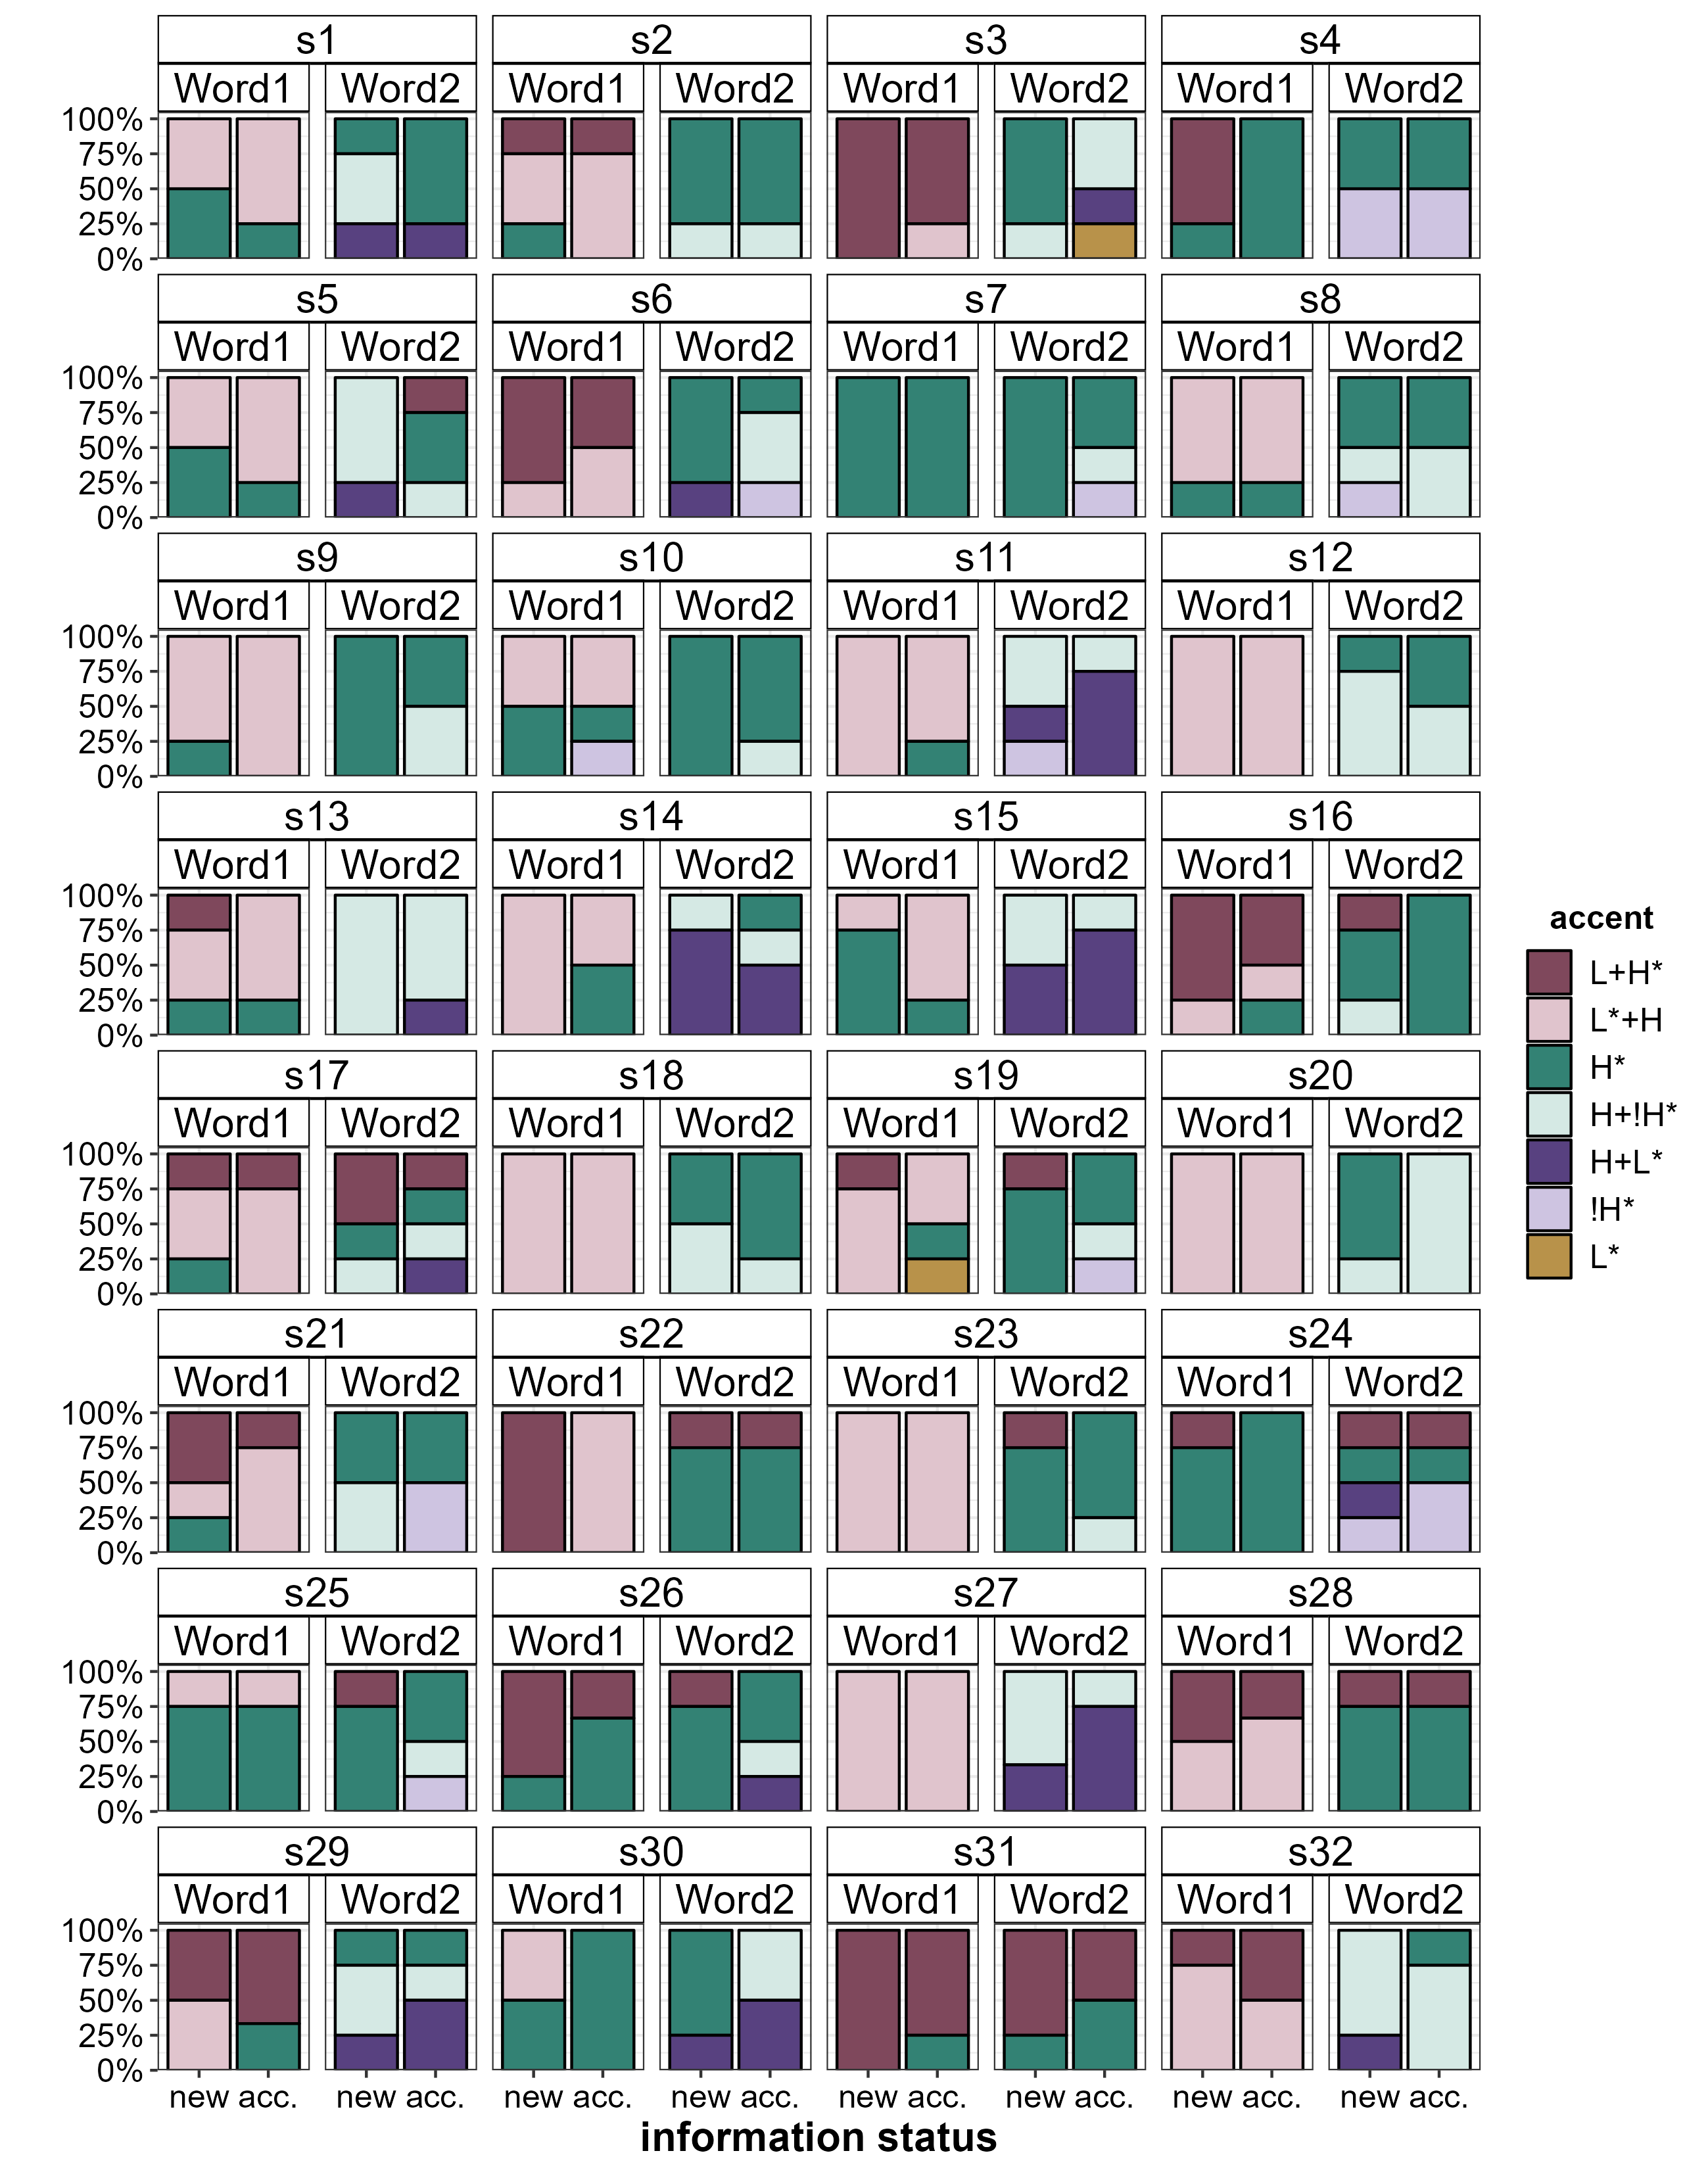
\includegraphics[scale = 0.55]{s1_accent_type_byspeaker_all}
	\caption{Barplots of the distributions of accent type by position and information status for each speaker.}	\label{fig:s1_accent_type_byspeaker_all}
\end{figure}

\chapter{Supplement to Production Study II} 
\label{Appendix B}

\section{Reading material}

\textbf{Story 1}: Banane `banana'\\
\\
Schon seit vielen Jahren arbeitet Susanne im Zoo als Tierpflegerin. Dort ist sie sehr glücklich und kümmert sich liebevoll um alle ihre Schützlinge. Heute hat Susanne \textbf{eine Banane} (1) mitgebracht. Sie hatte eine große Kiste mit viel Obst und Gemüse dabei und besonders die Affen waren ganz aufgeregt. Dann hat Susanne \textbf{die Banane} (2) herausgeholt. Sofort versammelten sich die Affen um sie. \textbf{Die Banane} (3) sah richtig lecker aus und der kleine Affe Tobi wollte sie unbedingt haben. Erst vor ein paar Tagen hatte ein Mädchen mit seinen Eltern vor dem Affengehege gestanden und Tobi beobachtet. Dabei hat das Mädchen \textbf{eine Banane} (4) gegessen. Da konnte Tobi die schöne gelbe Frucht nur ansehen, aber jetzt will er endlich eine probieren! \textbf{Die Banane} (5) wird er bestimmt sehr genießen.\\
\\
\textbf{Story 2}: Gardine `curtain'\\
\\
Sarah hat eine Arbeitsstelle in einer anderen Stadt bekommen und muss jetzt umziehen. Um ihre neue Wohnung einzurichten, war sie im Möbelhaus einkaufen. Dort hat Sarah \textbf{eine Gardine} (1) gefunden. Sie wollte eigentlich erst die Möbel aussuchen und sich dann um die restliche Einrichtung kümmern, sie hat sich aber im Möbelhaus verlaufen. Dabei hat Sarah \textbf{die Gardine} (2) gesehen. Der Preis passt gerade noch in das Budget für die Wohnung. \textbf{Die Gardine} (3) ist hellblau und hat die perfekte Länge für die Fenster im Wohnzimmer. Vorige Woche hatten Sarah und ihre beste Freundin schon zusammen im Internet recherchiert. Dabei hat ihre Freundin \textbf{eine Gardine} (4) vorgeschlagen. Die würde zwar gut ins Schlafzimmer passen, allerdings nicht ins Wohnzimmer. Aber zum Glück ist Sarah ja inzwischen fündig geworden! \textbf{Die Gardine} (5) wird sie noch heute Abend aufhängen.\\
\\
\textbf{Story 3}: Parade `parade'\\
\\
Um seinen Abschluss zu feiern, hat Julian einen Städtetrip unternommen. Er ist mit dem Zug nach Paris gefahren, hat im Hotel eingecheckt und wollte dann die Stadt erkunden. An dem Tag hat Julian \textbf{eine Parade} (1) eingeplant. Er wusste, dass ein Feiertag war und ist sofort in die Innenstadt gefahren. Dort hat Julian \textbf{die Parade} (2) angeschaut. Die Stimmung in der Stadt war super und die Straßen waren voll mit feiernden Menschen. \textbf{Die Parade} (3) war sehr groß und sah professionell aus. Letztes Jahr hat Julian einen Freund in dessen Heimatstadt zum Karneval besucht. Dort hat sein Freund \textbf{eine Parade} (4) organisiert. Die war allerdings sehr klein und ziemlich langweilig. Dieses Mal war Julian aber richtig beeindruckt! \textbf{Die Parade} (5) wird er nie vergessen.\\
\\
\textbf{Story 4}: Garage `garage'\\
\\
Peter wohnt seit einem Jahr in einem neuen Haus, das ihm gut gefällt. Es gibt nur ein Problem: Sein Auto parkt direkt unter einem Baum, wo immer viele Vögel sitzen. Jeden Morgen ist sein Auto dreckig – womit nun allerdings Schluss ist. Heute hat Peter \textbf{eine Garage} (1) gebaut. Er hat lange im Internet nach verschiedenen Bauplänen gesucht. Dann hat Peter \textbf{die Garage} (2) entworfen. Am Wochenende ist er in den Baumarkt gefahren und hat das notwendige Material gekauft. \textbf{Die Garage} (3) ist nämlich aus Metall und relativ groß. Die Idee dazu hat Peter von einem Kollegen bekommen, der vor Kurzem auf einer Architektur-Ausstellung war. Dort hat der Kollege \textbf{eine Garage} (4) gesehen. Peter war sich damals schon sicher, dass er mit all seiner Erfahrung genau so etwas nachbauen könnte. Jetzt hat er es geschafft und ist sehr zufrieden mit dem Ergebnis. \textbf{Die Garage} (5) wird er sicher jeden Tag benutzen.\\
\\
\textbf{Story 5}: Kombüse `galley'\\
\\
Heute war eine Schulklasse zu Besuch im Schifffahrtsmuseum. Ein Mitarbeiter hat den Schülern auf einem Rundgang alles erklärt, was sie wissen wollten. Direkt am Anfang hat die Klasse \textbf{eine Kombüse} (1) besichtigt. In diesem Museum sind nämlich alle Räume auf einem Schiff originalgetreu nachgebildet. Vorsichtig hat die Klasse \textbf{die Kombüse} (2) betreten. Darin waren die Figur eines Kochs, ein Herd, ein Ofen und viele Töpfe und Pfannen zu sehen. \textbf{Die Kombüse} (3) war viel kleiner als die Schüler erwartet hatten. Sie haben auch schon in der Schule einiges über Schiffe gelernt. Dabei hat die Lehrerin \textbf{eine Kombüse} (4) vorgestellt. Die war allerdings Teil eines großen Kriegsschiffs. Ein kleines Schiff wie das im Museum muss den begrenzten Platz strategisch gut ausnutzen und die Kinder wussten, dass viele Dinge an Bord wichtiger waren als das Kochen. \textbf{Die Kombüse} (5) haben sie aber auf jeden Fall interessant gefunden.\\
\\
\textbf{Story 6}: Praline `chocolate candy'\\
\\
Maria hat im Büro eine Kollegin, mit der sie sehr gut befreundet ist. Fast jeden Tag hat sie ein kleines Geschenk für Maria dabei, das sie ihr in der Mittagspause überreicht. Heute hat die Kollegin \textbf{eine Praline} (1) mitgebracht. Maria war noch am Arbeiten, als die Kollegin zu ihr an den Schreibtisch kam. Dann hat die Kollegin \textbf{die Praline} (2) ausgepackt. Sie war von einer edlen Marke und Maria hat sich sehr gefreut. \textbf{Die Praline} (3) war mit Karamell und Nüssen gefüllt. Als Kind war sie mit Süßigkeiten sehr wählerisch, was auch mit einem Erlebnis auf ihrem achten Geburtstag zusammenhängt. Damals hat Maria \textbf{eine Praline} (4) gegessen. Sie hat aber nicht gewusst, dass die manchmal mit Alkohol gefüllt sind. Maria hat sich geekelt und danach sehr lange gar keine Schokolade mehr angerührt. Diese Zeiten sind zum Glück vorbei und heute liebt Maria Schokolade aller Art. \textbf{Die Praline} (5) wird sie gleich als Vorspeise essen.\\
\\
\textbf{Story 7}: Ballade `ballad'\\
\\
Zum Valentinstag ist Max mit seiner Freundin ins Theater gegangen, um sich ein Musical anzusehen. Der Hauptdarsteller war weltbekannt und hatte schon viele Preise gewonnen. Max hat sich schon seit Wochen auf diesen Abend gefreut. Gleich am Anfang hat der Darsteller \textbf{eine Ballade} (1) gesungen. Das Licht wurde gedimmt und der Vorhang ging langsam auf. Dann hat der Darsteller \textbf{die Ballade} (2) begonnen. Er war ein Bariton und hatte eine wunderschöne Stimme. \textbf{Die Ballade} (3) war der Höhepunkt des Musicals. Früher war Max auch in einer Theatergruppe und hat sogar selber schon einmal bei einem Musical mitgemacht. Darin hat Max \textbf{eine Ballade} (4) vorgetragen. Es war eine große Herausforderung und er musste sehr lange üben, um sie zu perfektionieren. Aber der Darsteller in diesem Musical hat scheinbar mühelos gesungen. Das Stück hat Max so gut gefallen, dass er die CD mit der Musik gekauft hat. \textbf{Die Ballade} (5) wird er auf jeden Fall zuhause noch einige Male anhören.

\newpage
\textbf{Story 8}: Limone `lemon'\\
\\
Theo hat eine Nachbarin mit einem sehr großen Garten, die ihre Erzeugnisse regelmäßig an die Nachbarschaft verschenkt. Auch heute stand wieder eine Kiste vor seiner Tür. Unter anderem hat Theo \textbf{eine Limone} (1) bekommen. Der Zeitpunkt war ideal, weil er gerade alle seine Vorräte aufgebraucht hatte. Gut gelaunt hat Theo \textbf{die Limone} (2) herausgeholt. Alles in der Kiste sah sehr appetitlich aus. \textbf{Die Limone} (3) war ganz fest und leuchtend gelb. Theos Freundin geht oft auf dem Markt einkaufen, wo es jetzt im Sommer viele saisonale Angebote gibt. Letzte Woche hat seine Freundin \textbf{eine Limone} (4) gekauft. Die war zwar auch nicht schlecht, aber kein Vergleich zu dem Obst von seiner Nachbarin. Heute will Theo deshalb etwas tun, um sich bei ihr zu bedanken. \textbf{Die Limone} (5) wird er in einem Kuchen verarbeiten und seine Nachbarin zum Kaffee einladen.\\

\largerpage
\textbf{Practice story 1}: Makrele `mackerel'\\
\\
Paul wohnt an der Nordseeküste und an klaren Sommertagen geht er immer fischen. Auch heute ist er mal wieder mit seinem Boot aufs Meer gefahren. Nach einer Weile hat Paul \textbf{eine Makrele} (1) gefangen. Er hat gemerkt, dass sich sein Fischernetz bewegt und hat es eingeholt. Dann hat Paul \textbf{die Makrele} (2) herausgenommen. Sonst hingen nur Plastiktüten und Algen in seinem Netz. \textbf{Die Makrele} (3) war immerhin schön groß und gesund. Er hatte auch schon eine Idee, was er damit machen kann. Letzte Woche war er bei einer Freundin eingeladen. Zum Mittag hat die Freundin \textbf{eine Makrele} (4) gekocht. Die Mahlzeit war sehr lecker und hat ihn schwer beeindruckt. Paul will das Rezept jetzt auch selbst ausprobieren. \textbf{Die Makrele} (5) wird es auf jeden Fall heute zum Abendessen geben.\\
\\
\textbf{Practice story 2}: Rosine `raisin'\\
\\
Emma hatte letzte Woche Besuch von einem Freund, der selbstgebackene Plätzchen mitgebracht hatte. Sie war begeistert und hat sofort ein Plätzchen probiert. Dabei hat Emma \textbf{eine Rosine} (1) geschmeckt. Das war eine unangenehme Überraschung, weil die Stücke in den Plätzchen nach Schokolade aussahen. Dann hat Emma \textbf{die Rosine} (2) ausgespuckt. Es war ihr ein bisschen peinlich, aber ihr Freund war zum Glück gerade abgelenkt. \textbf{Die Rosine} (3) war sehr süß und ein bisschen klebrig. Seit Emma ein Kind war, hat sie eine starke Abneigung gegen getrocknete Früchte. Ihre Mutter hat sie aber immer dazu ermuntert, erstmal alles zu probieren, um sich eine eigene Meinung zu bilden. Also hat Emma \textbf{eine Rosine} (4) gegessen. Danach war sie sehr wütend auf ihre Mutter. Inzwischen kann sie ihren Standpunkt zwar nachvollziehen, aber sie möchte trotzdem nicht alles ausprobieren, was man ihr vorsetzt. \textbf{Die Rosine} (5) wird sie heute sicher nicht mehr essen.

\section{Communicative skill questionnaire}


Subset of questions related to communicative skill from the Autism-Spectrum Quotient questionnaire by \citet{baron-cohenAutismSpectrumQuotientAQ2006}, German translation from \url{https://autismus-kultur.de/autismus-asperger-test-erwachsene/}. Participants respond with “stimme voll zu" (`fully agree'), “stimme eher zu” (`rather agree'), “stimme eher nicht zu” (`rather disagree') or “stimme nicht zu” (`fully disagree').

``Fully disagree” or “rather disagree” responses scored 1 point on the following items: 1, 2, 3, 4, 5, 6. “Fully agree” or “rather agree” responses scored 1 point on the following items: 7, 8, 9, 10.

\begin{enumerate}
\item Andere Menschen sagen mir oft, dass das, was ich gesagt habe, unhöflich war, obwohl ich denke, es sei höflich gewesen.\\
`Other people frequently tell me that what I’ve said is impolite, even though I think it is polite.'
\item Wenn ich rede, ist es für andere nicht immer einfach, zu Wort zu kommen.\\
`When I talk, it isn’t always easy for others to get a word in edgeways.'
\item Ich stelle oft fest, dass ich nicht weiß, wie ich ein Gespräch in Gang halten kann.\\
`I frequently find that I don’t know how to keep a conversation going.'
\item Wenn ich am Telefon mit jemandem spreche, weiß ich nicht genau, wann ich wieder mit Sprechen an der Reihe bin.\\
`When I talk on the phone, I’m not sure when it’s my turn to speak.'
\item Ich verstehe einen Witz oft als Letzte/r.\\
`I am often the last to understand the point of a joke.'
\item Andere Leute sagen mir oft, dass ich ständig über dieselben Dinge spreche.\\
`People often tell me that I keep going on and on about the same thing.'
\item Ich genieße Smalltalk und belangloses Geplauder.\\
`I enjoy social chit-chat.'
\item Es fällt mir leicht, “zwischen den Zeilen zu lesen”, wenn sich jemand mit mir unterhält.\\
`I find it easy to “read between the lines” when someone is talking to me.'
\item Wenn ich mit jemandem rede, merke ich, wenn es ihm/ihr langweilig wird.\\
`I know how to tell if someone listening to me is getting bored.'
\item Smalltalk fällt mir leicht.\\
`I am good at social chit-chat.'
\end{enumerate}

\chapter{Supplement to Perception Study} 
\label{Appendix C}
\largerpage[2]

% \section{Predicted prominence ratings for continuous prosodic parameters}
\begin{figure}
	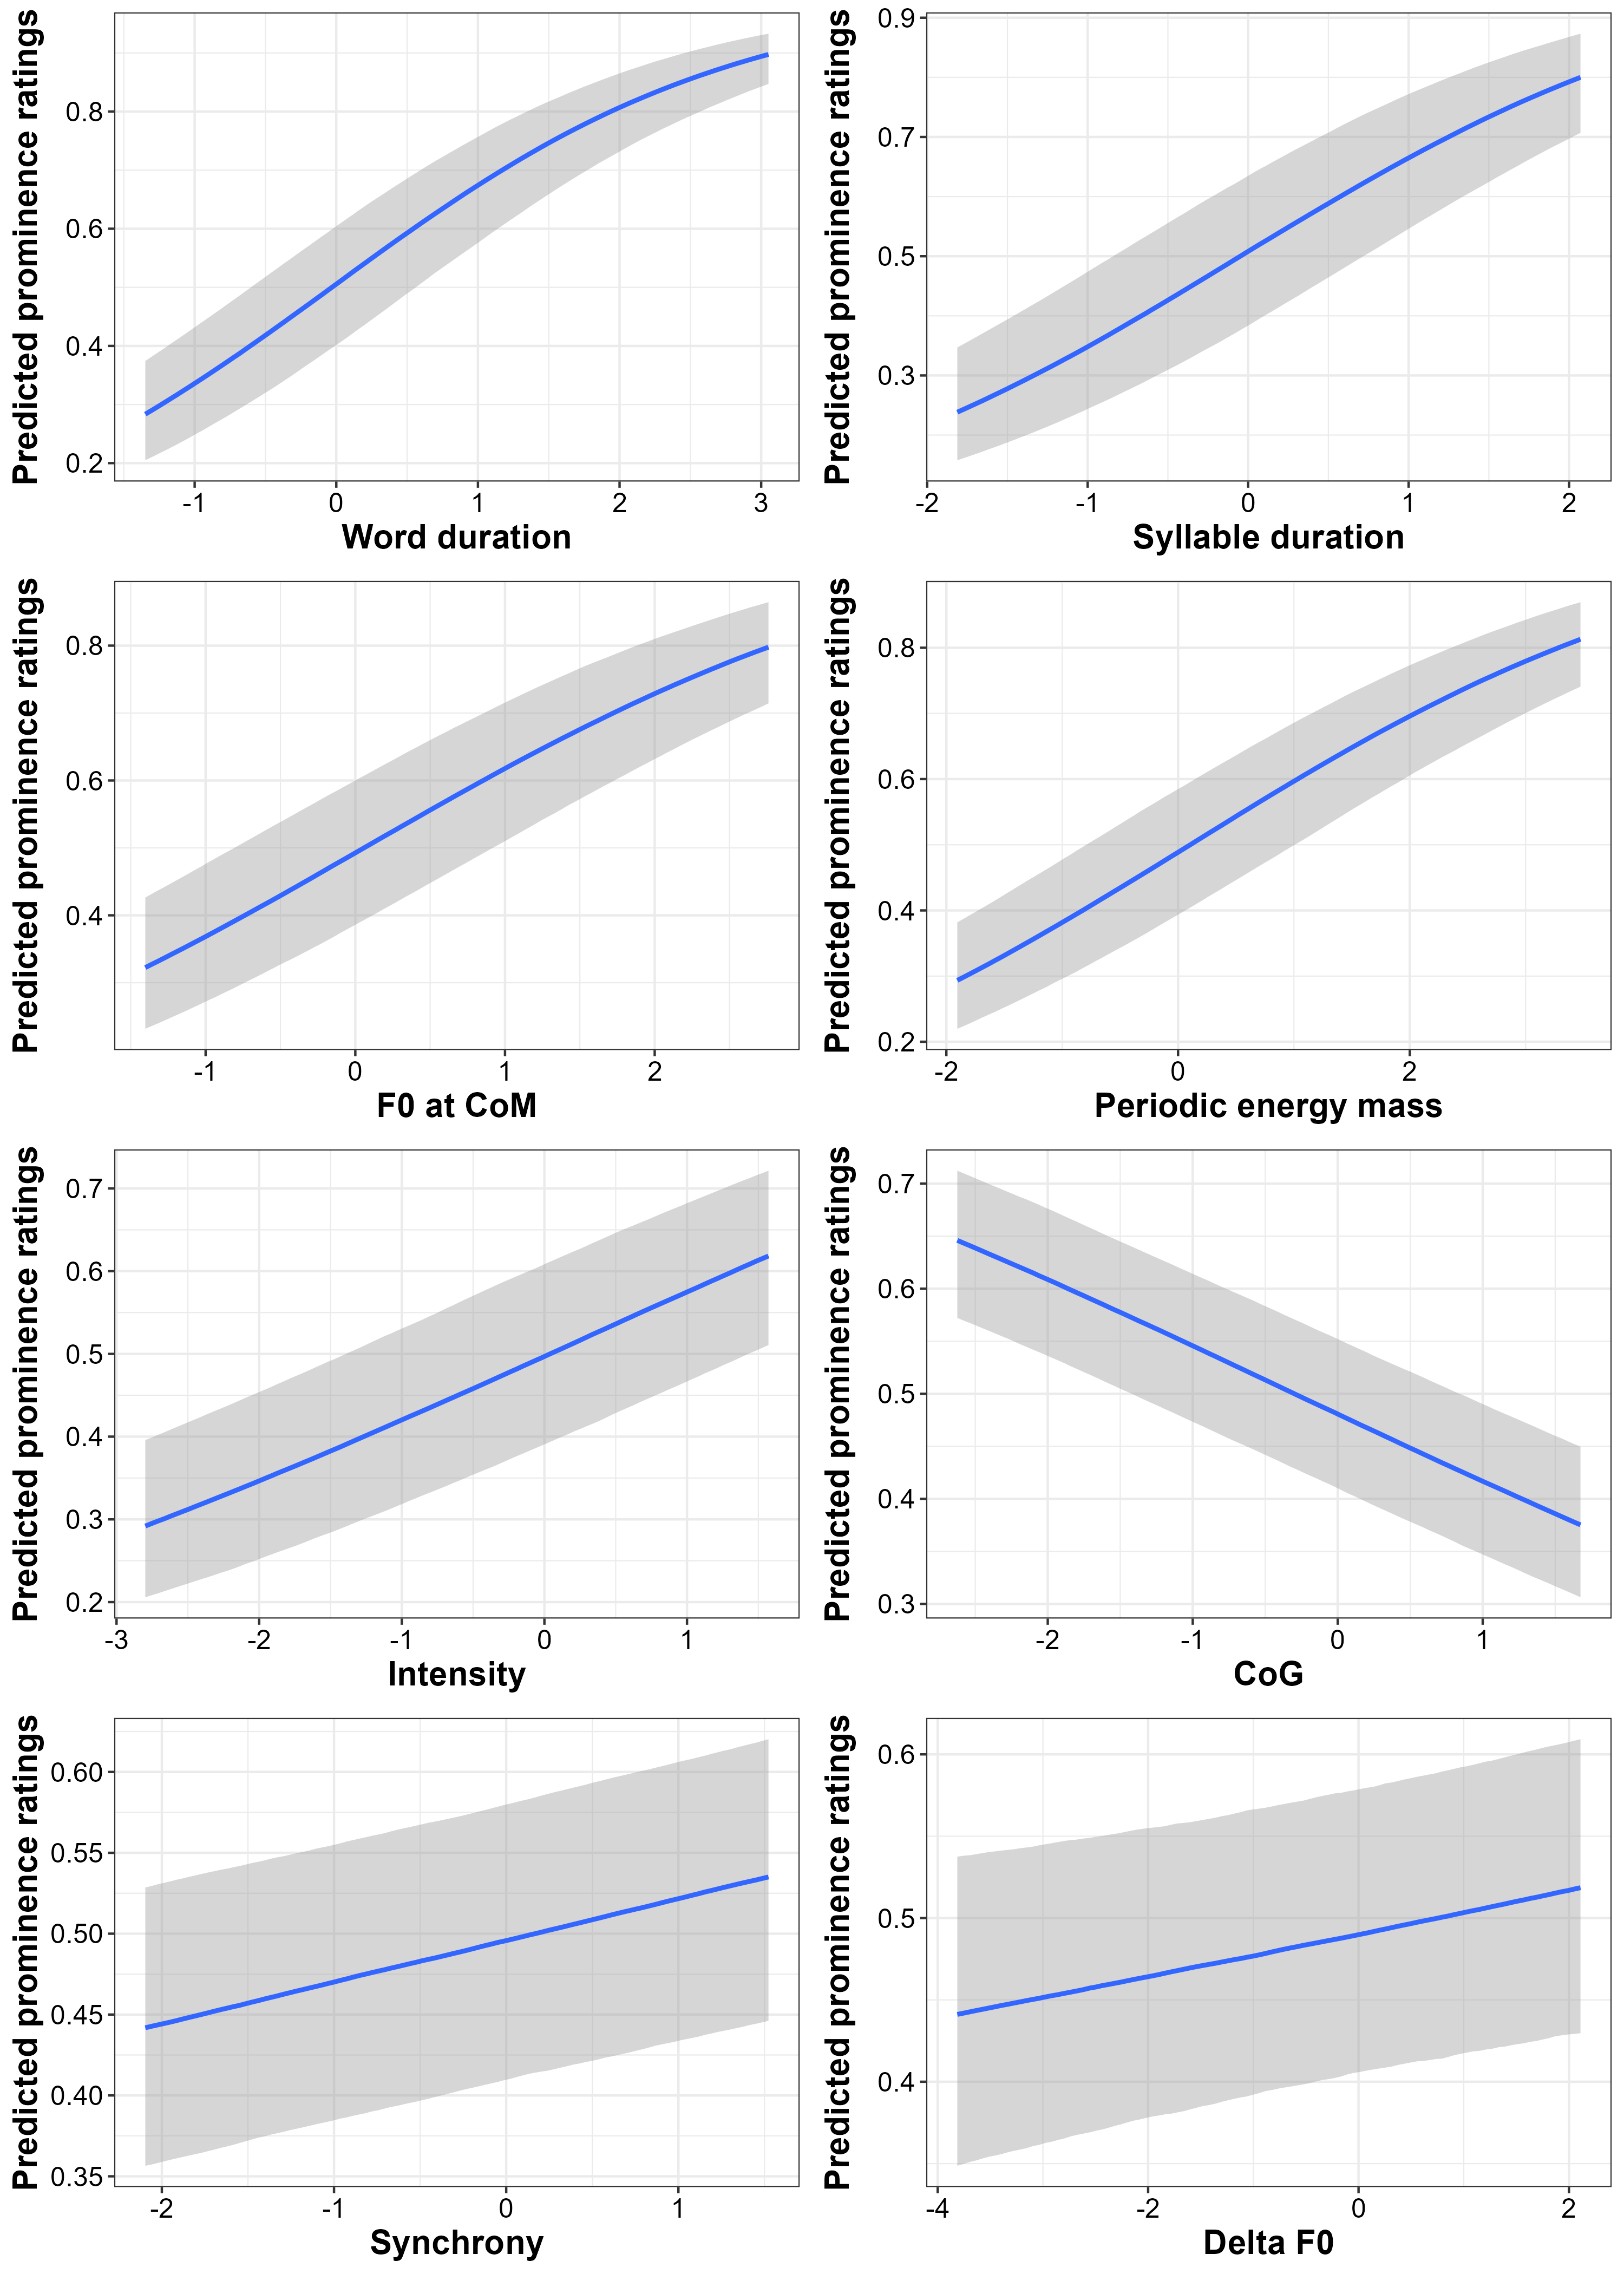
\includegraphics[width=.75\textwidth]{s3_cont_prmtrs_maineffects}
	\caption{Mean predicted prominence ratings and 90\% CrIs by continuous prosodic parameters.}
	\label{fig:s3_cont_prmtrs_maineffects}
\end{figure}


%%%%%%%%%%%%%%%%%%%%%%%%%%%%%%%%%%%%%%%%%%%%%%%%%%%
%%             Backmatter                       %%%
%%%%%%%%%%%%%%%%%%%%%%%%%%%%%%%%%%%%%%%%%%%%%%%%%%%

% \input{localseealso.tex}
% % There is normally no need to change the backmatter section
\backmatter
\phantomsection%this allows hyperlink in ToC to work
{\sloppy\printbibliography[heading=references]}
\cleardoublepage

\phantomsection
\addcontentsline{toc}{chapter}{\lsIndexTitle}
\addcontentsline{toc}{section}{\lsNameIndexTitle}
\ohead{\lsNameIndexTitle}
\printindex
\cleardoublepage

% \phantomsection
% \addcontentsline{toc}{section}{\lsLanguageIndexTitle}
% \ohead{\lsLanguageIndexTitle}
% \printindex[lan]
% \cleardoublepage
%
% \phantomsection
% \addcontentsline{toc}{section}{\lsSubjectIndexTitle}
% \ohead{\lsSubjectIndexTitle}
% \printindex[sbj]
% \ohead{}

\end{document} 
